\documentclass{article}
\usepackage[utf8]{inputenc}
\usepackage[greek,english]{babel}
\usepackage{alphabeta}
\usepackage{graphicx}
\usepackage{hyperref} 
\usepackage{listings}
\usepackage{booktabs}
\usepackage{subcaption}
\usepackage{mathtools}
\usepackage{amsmath}
\usepackage{array}
\date{\vspace{-4ex}}
\usepackage{relsize}
\title{Συστήματα Μικροϋπολογιστών}
\usepackage[svgnames]{xcolor} 

\addto\captionsenglish{% Replace "english" with the language you use
  \renewcommand{\contentsname}%
    {Περιεχόμενα}%
}

\def\changemargin#1#2{\list{}{\rightmargin#2\leftmargin#1}\item[]}
\let\endchangemargin=\endlist 

\usepackage{collectbox}

\makeatletter
\newcommand{\sqbox}{%
    \collectbox{%
        \@tempdima=\dimexpr\width-\totalheight\relax
        \ifdim\@tempdima<\z@
            \fbox{\hbox{\hspace{-.5\@tempdima}\BOXCONTENT\hspace{-.5\@tempdima}}}%
        \else
            \ht\collectedbox=\dimexpr\ht\collectedbox+.5\@tempdima\relax
            \dp\collectedbox=\dimexpr\dp\collectedbox+.5\@tempdima\relax
            \fbox{\BOXCONTENT}%
        \fi
    }%
}
\makeatother

\usepackage{graphicx}% just for the example text


\usepackage{blindtext}













\newcommand*{\plogo}{\fbox{$\mathcal{PL}$}} 
\begin{document}
   
\begin{titlepage} 
	
	\centering  
	
	\rule{\textwidth}{1pt} 
	
	\vspace{0.025\textheight}  
	ΑΡΙΣΤΟΤΕΛΕΙΟ ΠΑΝΕΠΙΣΤΗΜΙΟ ΘΕΣΣΑΛΟΝΙΚΗΣ
ΤΜΗΜΑ ΗΛΕΚΤΡΟΛΟΓΩΝ ΜΗΧΑΝΙΚΩΝ
ΚΑΙ ΜΗΧΑΝΙΚΩΝ ΥΠΟΛΟΓΙΣΤΩΝ
ΤΟΜΕΑΣ ΗΛΕΚΤΡΟΝΙΚΗΣ ΚΑΙ ΥΠΟΛΟΓΙΣΤΩΝ 
	
	\vspace{0.1\textheight}  
	
	\textcolor{black}{  
		{\Huge ΣYΝΘΕΣΗ
ΕΝΕΡΓΩΝ ΚΑΙ \\[0.5\baselineskip] ΠΑΘΗΤΙΚΩΝ
ΚYΚΛΩΜΑΤΩΝ}\\[0.5\baselineskip] 
		 % Title line 2
		 % Title line 3
	}
	
	\vspace{0.025\textheight}  
	
	\rule{0.3\textwidth}{0.4pt}  
	
	\vspace{0.1\textheight}  
	
 
	{\Large \textsc{\textbf{\underline{ΕΡΓΑΣΙΑ \#1,\#2,\#3,\#4}}}}  \\[1\baselineskip] \large{ΕΙΣΗΓΗΤΗΣ: ΘΕΟΧΑΡΗΣ Ι.} \\[1\baselineskip] 7ο ΕΞΑΜΗΝΟ  \\[2\baselineskip] Όνομα : Ιωάννης-Παναγιώτης Μπουντουρίδης \\[0.4\baselineskip] Α.Ε.Μ. : 8872
	\vfill  
 
 
	
	
	 

\vspace{2pt}\vspace{-\baselineskip}	
	ΘΕΣΣΑΛΟΝΙΚΗ 2019
	
	 
	
	\rule{\textwidth}{1pt} 
	
\end{titlepage}
\newpage
\begin{center}
\large{}

\tableofcontents
 
\newpage
\section*{ΣΥΝΘΕΣΗ ΕΝΕΡΓΩΝ ΚΑΙ ΠΑΘΗΤΙΚΩΝ ΚΥΚΛΩΜΑΤΩΝ} 
\end{center}
\section*{Εργασία \#1 Σχεδίαση Κατωδιαβατών φίλτρων}
\addcontentsline{toc}{section}{Εργασία \#1 Σχεδίαση Κατωδιαβατών φίλτρων}
\begin{equation*}
\\
\end{equation*}

\begin{center}
ΚΑΤΩΔΙΑΒΑΤΟ ΦΙΛΤΡΟ CHEBYCHEV
\end{center}
\large{}
Να σχεδιασθεί ένα κατωδιαβατό φίλτρο Chebychev το οποίο να πληροί τις παρακάτω προδιαγραφές συχνότητας και απόσβεσης : \\[0.4\baselineskip]
$f_p$ = 6KHz    ,      $f_s$ = 10.32KHz  , \\[0.4\baselineskip]
και \\[0.4\baselineskip]
$a_{max}$ =0.35 dB   ,     $a_{min}$ = 25,5 dB 
\subsection*{A. Αναλυτική Σχεδίαση του Φίλτρου}
\addcontentsline{toc}{subsection}{A. Αναλυτική Σχεδίαση του Φίλτρου} 
 
  \subsection*{$\bullet$Υπολογισμός της Συνάρτησης Μεταφοράς}
 
 \addcontentsline{toc}{subsection}{$\bullet$Υπολογισμός της Συνάρτησης Μεταφοράς} 

Στο πλαίσιο της διαδικασίας σχεδίασης θα πρέπει αρχικά να υπολογίσουμε την τάξη του φίλτρου που απαιτείται. Για να γίνει αυτό θα χρησιμοποιήσουμε τον παρακάτω τύπο :
\begin{equation}
\boxed{n=\frac{cosh^{-1}[(10^{{α_{min}}/{10}}-1)/ (10^{{α_{max}}/{10}}-1)]^{1/2}}{cosh^{-1}(Ω_s)}
}
\end{equation}
δεδομένων των $f_s$, $f_p$
\begin{equation*}
ω_s = 2πf_s \Rightarrow \boxed{ω_s =\enspace 64842 \enspace rad/s}
\end{equation*}
\begin{equation*}
ω_p = 2πf_p \Rightarrow \boxed{ω_p =\enspace 37699 \enspace rad/s}   
\end{equation*}
κανονικοποιούμε την συχνότητα $ω_p$ ώστε να πάρουμε $Ω_p$=1 και επομένως να έχουμε:
\begin{equation*}
\boxed{Ω_p = 1} \enspace \enspace \boxed{Ω_s = \frac{ω_s}{ω_p} = 1.72}
\end{equation*}
αντικαθιστώντας τις τιμές των προδιαγραφών στην (1) υπολογίζουμε: n = 4.277. Επειδή το n που προέκυψε δεν είναι ακέραιος επιλέγουμε τον αμέσως επόμενο. Δηλαδή $\boxed{n=5}$ \\[0.4\baselineskip]
Θα υπολογίσουμε τώρα την συχνότητα ημίσειας ισχύος από τον τύπο:
\begin{equation*}
\boxed{
Ω_{hp} = cosh\{\frac{1}{n}cosh^{-1}(10^{a_{max}/10} -1)^{-1/2}\} }
\end{equation*} 
αντικαθιστώντας τα n και $a_{max}$ βρίσκουμε $\boxed{Ω_{hp}=1.07388}$. \\
Έτσι λοιπόν έπειτα από αντικατάσταση θα έχουμε ότι η συχνότητα ημίσειας ισχύος $ω_{hp}$ είναι :
\begin{equation*}
f_{hp} = Ω_{hp} \cdot f_p \Rightarrow
\boxed{f_{hp} = 6.443 kHz}
\end{equation*}
\begin{equation*}
ω_{hp} = 2πf_{hp} \Rightarrow \boxed{ω_{hp} = 40484rad/s} 
\end{equation*}
H συνάρτηση απόσβεσης του φίλτρου Chebyshev ορίζεται ως:
\begin{equation*}
a_n = 10log(1+ε^2 {C_n}^2(ω))
\end{equation*}
Η μέγιστη τιμή της απόσβεσης $a_{max}$ στην ζώνη διόδου (0,1) συμβαίνει όταν ${C_n}^2$(ω)=1 οπότε έχουμε:
\begin{equation*}
a_{max} = 10log(1+ε^2) \Rightarrow \boxed{ε = \sqrt{10^{a_{max}/10} -1}}
\end{equation*}
κάνοντας αντικατάσταση το $a_{max}$ παίρνουμε $\boxed{ε = 0.2897}$\\ Απο την ανάλυση της θεωρείας γνωρίζουμε οτι: 
\begin{equation*}
v_k = \pm \frac{1}{n}sinh^{-1}(\frac{1}{ε}) = \pm α \Rightarrow α = \frac{1}{n}sinh^{-1}(\frac{1}{ε}) \Rightarrow \boxed{α = 0.3904}
\end{equation*}
\begin{equation*}
\boxed{cosha =1.0772} 
\end{equation*}
\begin{equation*}
  \boxed{sinha = 0.4004}
\end{equation*}
oι γωνίες Butterworth για n=5 είναι $ψ_κ$ = 0, $\pm36^o$, $\pm72^o$ 
\\ επομένως οι πόλοι θα είναι:
\begin{align*}
-σ_k = sinha \cdot cosψ_k \\
\pm ω_k = cosha \cdot sin ψ_k \\
\end{align*}
κάνοντας αντικατάσταση τις γωνίες προκύπτει:
\begin{align*}
σ_1 = -0.4004 \enspace και \enspace ω_1 = 0 \\
\boxed{p_1 = -0.4004} \\
σ_{2,3} = - 0.3239 \enspace και \enspace ω_{2,3} = 0.6331 \\
\boxed{p_{2,3} = -0.3239 \pm 0.6331j} \\
σ_{4,5} = -0.1237 \enspace και \enspace ω_{4,5} = 1.0244\\
\boxed{p_{4,5} = -0.1237 \pm 1.0244j}
\end{align*}
θεωρούμε ένα ζεύγος πόλων
\begin{equation*}
(s+σ_k-jω_k)(s+σ_k+jω_k) = s^2 + 2σ_ks + ({σ_k}^2+{ω_k}^2)
\end{equation*}
εκφράζοντας τον όρο αυτό συναρτήσει των $ω_o$,Q έχουμε:
\begin{equation*}
s^2 + \frac{ω_0}{Q} s  + {ω_0}^2
\end{equation*}
\begin{equation*}
\boxed{{ω_0} = \sqrt{{σ_k}^2+{ω_k}^2}} \enspace 
\boxed{Q = \frac{\sqrt{{σ_k}^2 + {ω_k}^2}}{2σ_k}} 
\end{equation*}
αντικαθιστώντας τα $σ_k$, $ω_k$ βρίσκουμε:
\begin{align*}
Ω_{0_1} = 0.4004 \\
Ω_{0_{2,3}} = 0.7112 \\
Ω_{0_{4,5}} = 1.0319 \\
\end{align*}
τα πραγματικά μέτρα των πόλων είναι
\begin{equation*}
Ω_{0_1} = 2\cdot π \cdot 6000 \cdot 0.4004 \Rightarrow \boxed{Ω_{0_1} = 15098 rad/s}
\end{equation*}
\begin{equation*}
Ω_{0_{2,3}} = 2\cdot π \cdot 6000 \cdot 0.7112 \Rightarrow \boxed{Ω_{0_{2,3}} = 26813 rad/s}
\end{equation*}
\begin{equation*}
Ω_{0_{4,5}} = 2\cdot π \cdot 6000 \cdot 1.0319 \Rightarrow \boxed{Ω_{0_{4,5}} = 38903 rad/s}
\end{equation*}
αντικαθιστώντας τα $σ_k$, $ω_k$ βρίσκουμε:
\begin{equation*}
\boxed{Q_{{1}} =  0.5}
\end{equation*}
\begin{equation*}
\boxed{Q_{2,3} =  1.0976}
\end{equation*}
\begin{equation*}
\boxed{Q_{4,5} =  4.1692}
\end{equation*}
Οι πόλοι της συνάρτησης μεταφοράς , οι γωνίες καθώς και τα αντίστοιχα Q των ριζών προκύπτουν και παρουσιάζονται στον παρακάτω πίνακα:

 
\begin{center}

 \begin{tabular}{|c|c|c|}
        \hline
       \qquad $ψ_k$ \qquad \qquad &\qquad \qquad Q \qquad \qquad \qquad & \qquad \qquad $p_k$ \qquad \qquad \qquad \\
        \hline
        $0$ & 0.5 & -0.4004 \\
        \hline
        $\pm36^o$ & 1.0976 & $ -0.3239 \pm 0.6331j$\\
        \hline
        $\pm72^o$ & 4.1692 & $-0.1237 \pm 1.0244j$\\
        \hline
        \end{tabular}
\end{center}
Άρα η συνάρτηση μεταφοράς που πρέπει να υλοποιηθεί θα αποτελείται από 3 μονάδες οι οποίες και φαίνονται παρακάτω σε διαγραμματική μορφή. \\
\begin{center}
\raisebox{-6ex}{$\to$}%
\fbox{\parbox[t]{8em}{$\enspace$ \\ Μονάδα \#1\\ $Ω_{0_1} = 0.4004$ \\$Q_{{1}} =  0.5$ \\$\enspace$}}%
\raisebox{-6ex}{$\to$}%
\fbox{\parbox[t]{8em}{$\enspace$ \\ Μονάδα \#2\\ $Ω_{0_{2,3}} = 0.7112$ \\$Q_{2,3} =  1.0976$ \\$\enspace$}}%
\raisebox{-6ex}{$\to$}%
\fbox{\parbox[t]{8em}{$\enspace$ \\ Μονάδα \#3\\ $Ω_{0_{4,5}} =  1.0319$ \\$Q_{4,5} =  4.1692$ \\$\enspace$}}%
\raisebox{-6ex}{$\to$}%
\end{center} 
Το συνολικό κύκλωμα αποτελείται απο τρεις μονάδες. Η μονάδα (Ι) αντιστοιχεί στον πραγματικό πόλο $p_1$, η μονάδα (ΙΙ) αντιστοιχεί στο ζεύγος μιγαδικών $p_{2,3}$ και η μονάδα (ΙΙΙ) αντιστοιχεί στο ζεύγος πόλων $p_{4,5}$. Η πρώτη μονάδα είναι ενα παθητικό φίλτρο πρώτης τάξης και επόμενες δυο μονάδες είναι Sallen-Key (στρατιγική σχεδίασης 2). 
\newpage
  \subsection*{$\bullet$Υλοποίηση της Συνάρτησης Μεταφοράς}
 
 \addcontentsline{toc}{subsection}{$\bullet$Υλοποίηση της Συνάρτησης Μεταφοράς} 
Για την υλοποίηση της συνάρτησης μεταφοράς θα χρησιμοποιηθεί μια μονάδα παθητικού φίλτρο πρώτης τάξης και δυό μονάδες Sallen-Key με βάση την $\boxed{στρατηγικη \enspace σχεδίασης (2)}$ αφου $a_3$ = 7 \\ 
Η κλιμακοποίηση των φίλτρων να γίνει έτσι ώστε οι μονάδες
Sallen-Key
να έχουν έναν τουλάχιστον πυκνωτή με τιμή $\boxed{C = 1μF}$ αφού $a_4$ = 2
\\[0.4\baselineskip]
\large{ \underline{\textbf{Μονάδα Ι}} \\[0.4\baselineskip]}
\large{}
Θεωρούμε τα κανονικοποιημένα στοιχεία
\begin{equation*}
σ_1 = \frac{1}{RC} = 0.4004, αν \enspace R_{11} = 1 \enspace τοτε \enspace C_{11} = 2.497
\end{equation*}
\begin{equation*}
\boxed{ R_{11} = 1} \enspace \boxed{C_{11} = 2.497}
\end{equation*}
\large{ {\textbf{Κλιμακοποίηση}} \\[0.4\baselineskip]}
\large{}
Eπιλέγουμε $k_m$ = $10^4$ για αντιστάσεις 10KΩ, και λόγω κλιμακοποίησης συχνότητας $k_f=ω_p$ = 37699 οπότε $Α = \frac{1}{k_m k_f}$ = 2.65258 $\cdot 10^{-9}$  \\
επομένως $\boxed{R_{11} = 10KΩ}$ και $\boxed{C_{11} = 6.62nF}$ θα είναι τα πραγματικά στοιχεία της μονάδας
\\[0.4\baselineskip]
\large{ \underline{\textbf{Μονάδα ΙI}} \\[0.4\baselineskip]}
\large{}
Θεωρούμε προσωρινά ότι $Ω_{0_{2,3}} = 1$
\begin{equation*}
C_{21} = 2Q_{2,3} \Rightarrow \boxed{C_{21} = 2.1952}
\end{equation*}
\begin{equation*}
C_{22} = \frac{1}{2Q_{2,3}} \Rightarrow \boxed{C_{22} = 0.4555}
\end{equation*}
\begin{equation*}
R_{21} = R_{22} = 1 
\end{equation*}
\begin{equation*}
k=1
\end{equation*}
\\[0.4\baselineskip]
\large{ {\textbf{Κλιμακοποίηση}} \\[0.4\baselineskip]}
\large{}
Για την συχνότητα $k_f$ = $ω_{0_{2,3}} \cdot ω_p \Rightarrow$ $k_f$ = 26813 \\ 
Ζητούμενο των προδιαγραφών μας είναι να έχουμε τουλάχιστον έναν πυκνωτή με τιμή 1μF. \\
Για αυτό επιλέγουμε κατάλληλα την $k_m$:
\begin{equation*}
 k_m = \frac{2 \cdot }{k_f \cdot 1μF}Q_{2,3} \Rightarrow k_m = \frac{2 \cdot 10^6}{k_f}Q_{2,3}
\end{equation*}
\begin{equation*}
k_m = 81.871 
\end{equation*}
επομένως τα πραγματικά στοιχεία της μονάδας θα είναι:
\begin{equation*}
C_{21}= A \cdot 2.204 F \enspace  
\end{equation*}
\begin{equation*}
C_{22}= A \cdot 0.453 F \enspace  
\end{equation*}
αντικαθηστάμε οπου $Α = \frac{1}{k_m k_f}$ και παίρνουμε
\begin{equation*}
\boxed{C_{21}=1μF} \enspace \boxed{C_{22}=0.207μF}
\end{equation*}
\begin{equation*}
R_{21}= R_{22} = k_m \cdot 1
\end{equation*}
\begin{equation*}
\boxed{R_{21}= 81.871  Ω} \enspace \boxed{R_{22}= 81.871  Ω}
\end{equation*}

\large{ \underline{\textbf{Μονάδα IIΙ}} \\[0.4\baselineskip]}
\large{}
Θεωρούμε προσωρινά ότι $Ω_{0(3,4)} = 1$
\begin{equation*}
C_{31} = 2Q_{4,5} \Rightarrow \boxed{C_{31} = 8.3385}
\end{equation*}
\begin{equation*}
C_{32} = \frac{1}{2Q_{4,5}} \Rightarrow \boxed{C_{32} = 0.1199}
\end{equation*}
\begin{equation*}
R_{31} = R_{32} = 1 
\end{equation*}
\begin{equation*}
k=1
\end{equation*}
\\[0.4\baselineskip]
\large{ {\textbf{Κλιμακοποίηση}} \\[0.4\baselineskip]}
\large{}
Για την συχνότητα $k_f$ = $ω_{0_{4,5}}\cdot ω_p \Rightarrow$ $k_f$ = 38903 \\ 
Ζητούμενο των προδιαγραφών μας είναι να έχουμε τουλάχιστον έναν πυκνωτή με τιμή 1μF. \\
Για αυτό επιλέγουμε κατάλληλα την $k_m$:
\begin{equation*}
 k_m = \frac{2 \cdot }{k_f \cdot 1μF}Q_{4,5} \Rightarrow k_m = \frac{2 \cdot 10^6}{k_f}Q_{4,5}
\end{equation*}
\begin{equation*}
k_m = 214.341
\end{equation*}
επομένως τα πραγματικά στοιχεία της μονάδας θα είναι:
\begin{equation*}
C_{31}= A \cdot 8.3385 F \enspace  
\end{equation*}
\begin{equation*}
C_{32}= A \cdot 0.1199 F \enspace  
\end{equation*}
αντικαθηστάμε οπου $Α = \frac{1}{k_m k_f}$ και παίρνουμε
\begin{equation*}
\boxed{C_{31}=1μF} \enspace \boxed{C_{32}=14.3nF}
\end{equation*}
\begin{equation*}
R_{31}= R_{32} = k_m \cdot 1
\end{equation*}
\begin{equation*}
\boxed{R_{31}=214.341  Ω} \enspace \boxed{R_{32}=214.341 Ω}
\end{equation*}
\newpage
 \subsection*{$\bullet$Ρύθμιση κέρδους}
 
 \addcontentsline{toc}{subsection}{$\bullet$Ρύθμιση κέρδους} 
 
\normalsize{}
Μια ακόμη απαίτηση των προδιαγραφών είναι να γίνει ρύθμιση κέρδους έτσι ώστε το κέρδος του φίλτρου
στις χαμηλές συχνότητες να είναι: $\boxed{\enspace 0 \enspace dB \enspace} \enspace αφου \enspace a_2 =8$. \\
Το συνολικό κύκλωμα αποτελείται απο τρεις μονάδες. Η μονάδα (Ι) αντιστοιχεί στον πραγματικό πόλο $p_1$, η μονάδα (ΙΙ) αντιστοιχεί στο ζεύγος μιγαδικών $p_{2,3}$ και η μονάδα (ΙΙΙ) αντιστοιχεί στο ζεύγος πόλων $p_{4,5}$. Η πρώτη μονάδα είναι ενα παθητικό φίλτρο πρώτης τάξης και επόμενες δυο μονάδες είναι Sallen-Key (στρατιγική σχεδίασης 2). Επειδή οι μονάδες αυτές δίνουν κέρδος μονάδα στο dc όσο δηλαδή η προδιαγραφή που έχει τεθεί δεν απαιτείται περαιτέρο διόρθωση κέρδους στην τελική φάση.\\[0.4\baselineskip]
\large{ \underline{\textbf{Συναρτήσεις Μεταφοράς Μονάδων}} \\[0.4\baselineskip]
\large{}
1. Για την πρώτη μονάδα η συνάρτηση μεταφοράς είναι :
\begin{equation*}
T_1(s) = \frac{{Ω_{0_{1}}}}{s+Ω_{0_{1}}} \Rightarrow
\end{equation*}
 \begin{equation*}
\boxed{T_1(s) = \frac{15098}{s+15098} }
\end{equation*}
2. Για την δεύτερη μονάδα η συνάρτηση μεταφοράς είναι :
\begin{equation*}
T_2(s) = \frac{{Ω_{0_{2,3}}}^2}{s^2+ \frac{Ω_{0_{2,3}}}{Q_{2,3}}s+ {Ω_{0_{2,3}}}^2} \Rightarrow
\end{equation*}
\begin{equation*}
\boxed{T_2(s) = \frac{718961620}{s^2+24428s+718961620}}
\end{equation*}
2. Για την τρίτη μονάδα η συνάρτηση μεταφοράς είναι :
\begin{equation*}
T_3(s) = \frac{{Ω_{0_{4,5}}}^2}{s^2+ \frac{Ω_{0_{4,5}}}{Q_{4,5}}s+ {Ω_{0_{4,5}}}^2} \Rightarrow
\end{equation*}
\begin{equation*}
\boxed{T_3(s) = \frac{1513449449}{s^2+9330s+1513449449}}
\end{equation*}
Η συνολική συνάρτηση μεταφοράς του κατωδιαβατού φίλτρου:
\begin{equation*}
T_{LP}(s) = Κ \cdot T_1(s) \cdot T_2(s), \enspace K=1
 \Rightarrow
\end{equation*}
\begin{equation*}
\boxed{T_{LP}(s) = \frac{1.643 \cdot 10^{22}}{(s+15097)(s^2+24428s+718961620)(s^2+9330s+1513449449)}}
\end{equation*}
\newpage
\section*{Παρουσίαση κανονικοποιημένου κυκλώματος}
Στο παρακάτω σχήμα φαίνεται το κανονικοποιημένο κύκλωμα στο οποίο παρουσιάζονται οι τρεις μονάδες που έχουν υλοποιηθεί.Η πρώτη μονάδα είναι ενα παθητικό φίλτρο πρώτης τάξης και επόμενες δυο μονάδες είναι Sallen-Key (στρατιγική σχεδίασης 2).

 \begin{figure*}[h!]
\centering
 	\advance\leftskip-4.9cm
  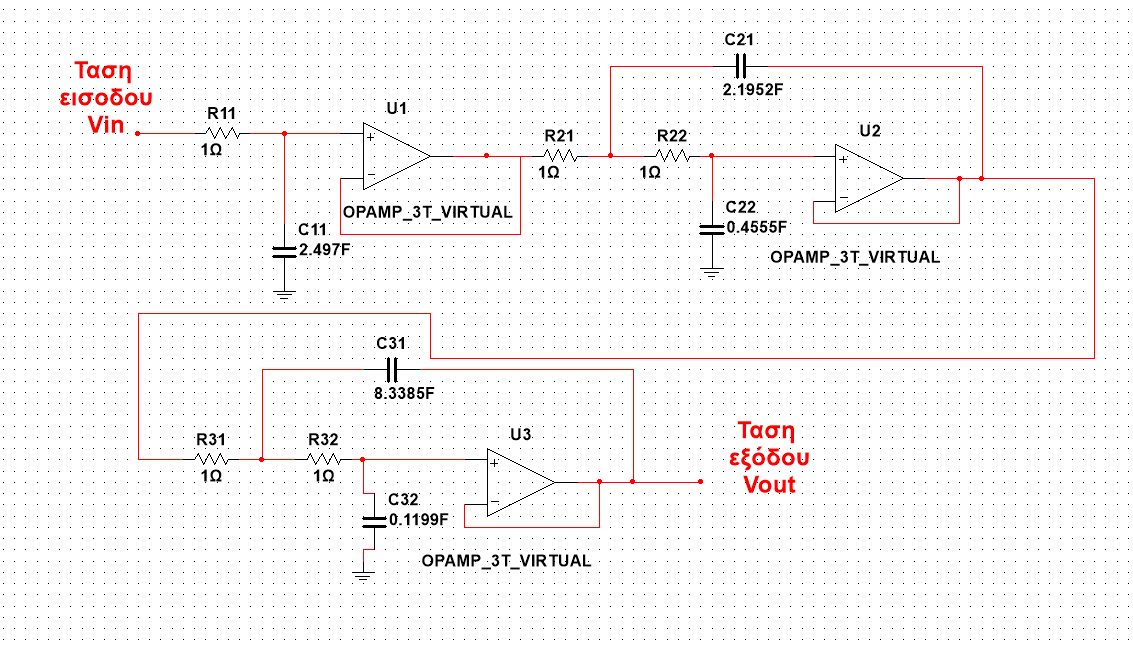
\includegraphics[width=220mm,scale=2]{kanonikopoiimeno_fixed.png}
  
  
 
\end{figure*}
\newpage
\section*{Παρουσίαση τελικού κυκλώματος}
   Εδώ βλέπουμε το τελικό κύκλωμα, το επιθυμητό δηλαδή κατωδιαβατό φίλτρο Chebyshev με ότι στοιχείο είναι απαραίτητο αλλά και με τις απαιτούμενες τιμές όλων των στοιχείων για την ικανοποίηση των ζητούμενων προδιαγραφών.
    \begin{figure*}[h!]
\centering
 \advance\leftskip-5.1cm
  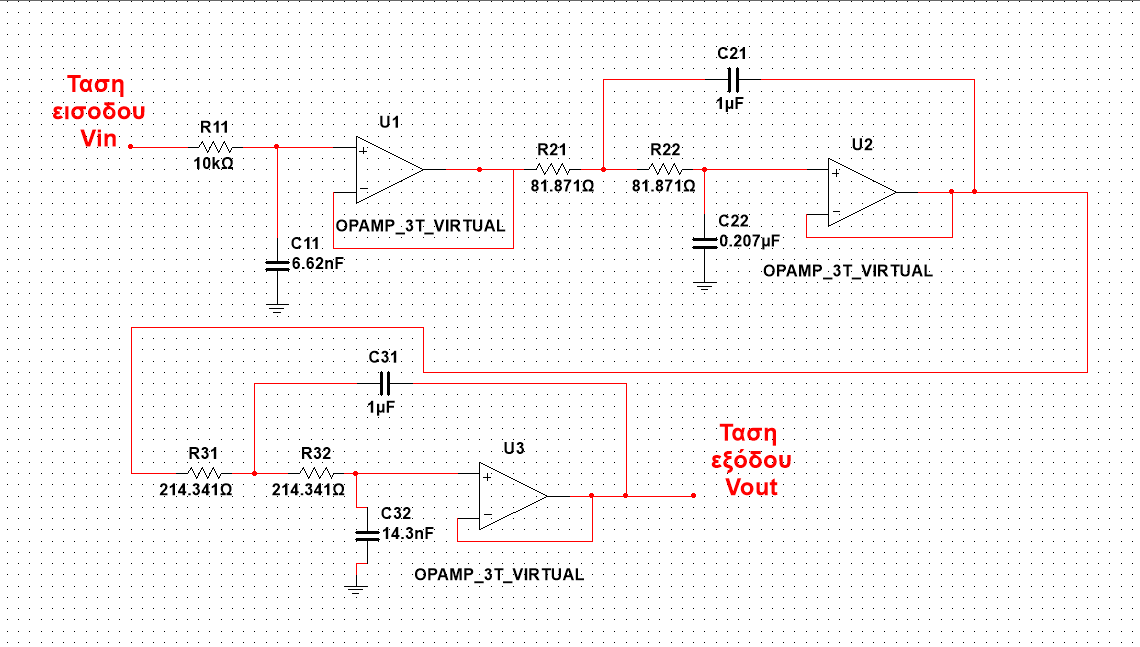
\includegraphics[width=220mm,scale=2]{telikok.png}
  
  
 
\end{figure*} 
\clearpage
\subsection*{B. Μελέτη της Συνάρτησης Μεταφοράς στο MATLAB}
\addcontentsline{toc}{subsection}{B. Μελέτη της Συνάρτησης Μεταφοράς στο MATLAB}
\large{}
Εισάγουμε στο  πρόγραμμα MATLAB τις επί μέρους συναρτήσεις μεταφοράς
 \begin{equation*}
\boxed{T_1(s) = \frac{15098}{s+15098} }
\end{equation*} 
\begin{equation*}
\boxed{T_2(s) = \frac{718961620}{s^2+24428s+718961620}}
\end{equation*}
\begin{equation*}
\boxed{T_3(s) = \frac{1513449449}{s^2+9330s+1513449449}}
\end{equation*}
αλλά και την συνολική συνάρτησης μεταφοράς του φίλτρου 
\begin{equation*}
\boxed{T_{LP}(s) = \frac{1.643 \cdot 10^{22}}{(s+15097)(s^2+24428s+718961620)(s^2+9330s+1513449449)}}
\end{equation*}
και παίρνουμε τις αποκρίσεις πλάτους σε dB. \\ Η απόκριση πλάτους σε dB για την πρώτη, την δεύτερη και την τρίτη μονάδα παρουσιάζονται ευθύς αμεσως. Τα παρακάτω διαγράμματα προέκυψαν στο Matlab χρησιμοποιώντας την παρεχόμενη συνάρτηση plot\_transfer\_function.m με όρισμα κάθε φορά την συνάρτηση μεταφοράς των επί μέρους συστημάτων, καθώς και τις κρίσιμες συχνότητες αυτών. 
\\[2.4\baselineskip]

\newpage
\section*{$1^\textbf{η}$ Μονάδα: Παθητικό φίλτρο πρώτης τάξης} 
  \begin{figure*}[h!]
\centering
 	\advance\leftskip-4cm
  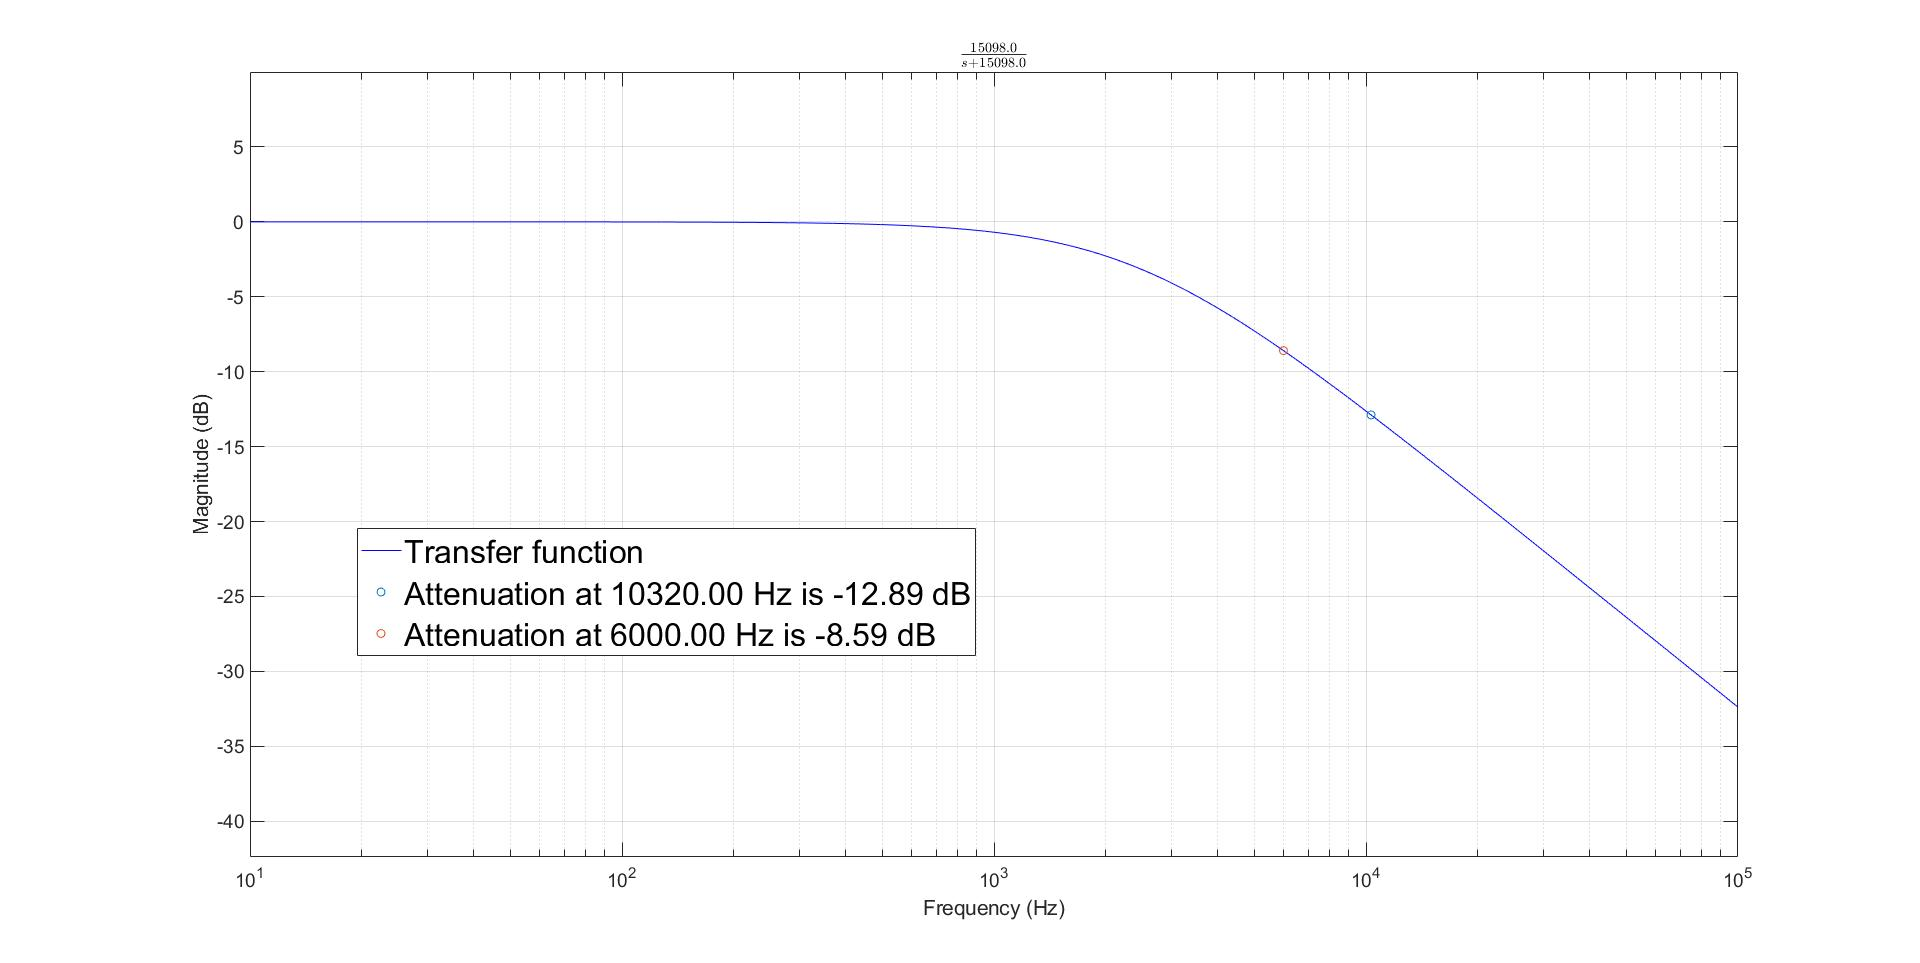
\includegraphics[width=200mm,scale=2]{t1.jpg}
\end{figure*}
\normalsize{}
Στο παραπάνω διάγραμμα της $1^{ης}$ μονάδας κάνουμε ζουμ ώστε να φαίνεται ευδιάκριτα η απόκριση στις κρίσημες συχνότητες με τις κατάλληλες κλίμακες:
\large{}
 \begin{figure*}[h!]
\centering
 	\advance\leftskip-1cm
  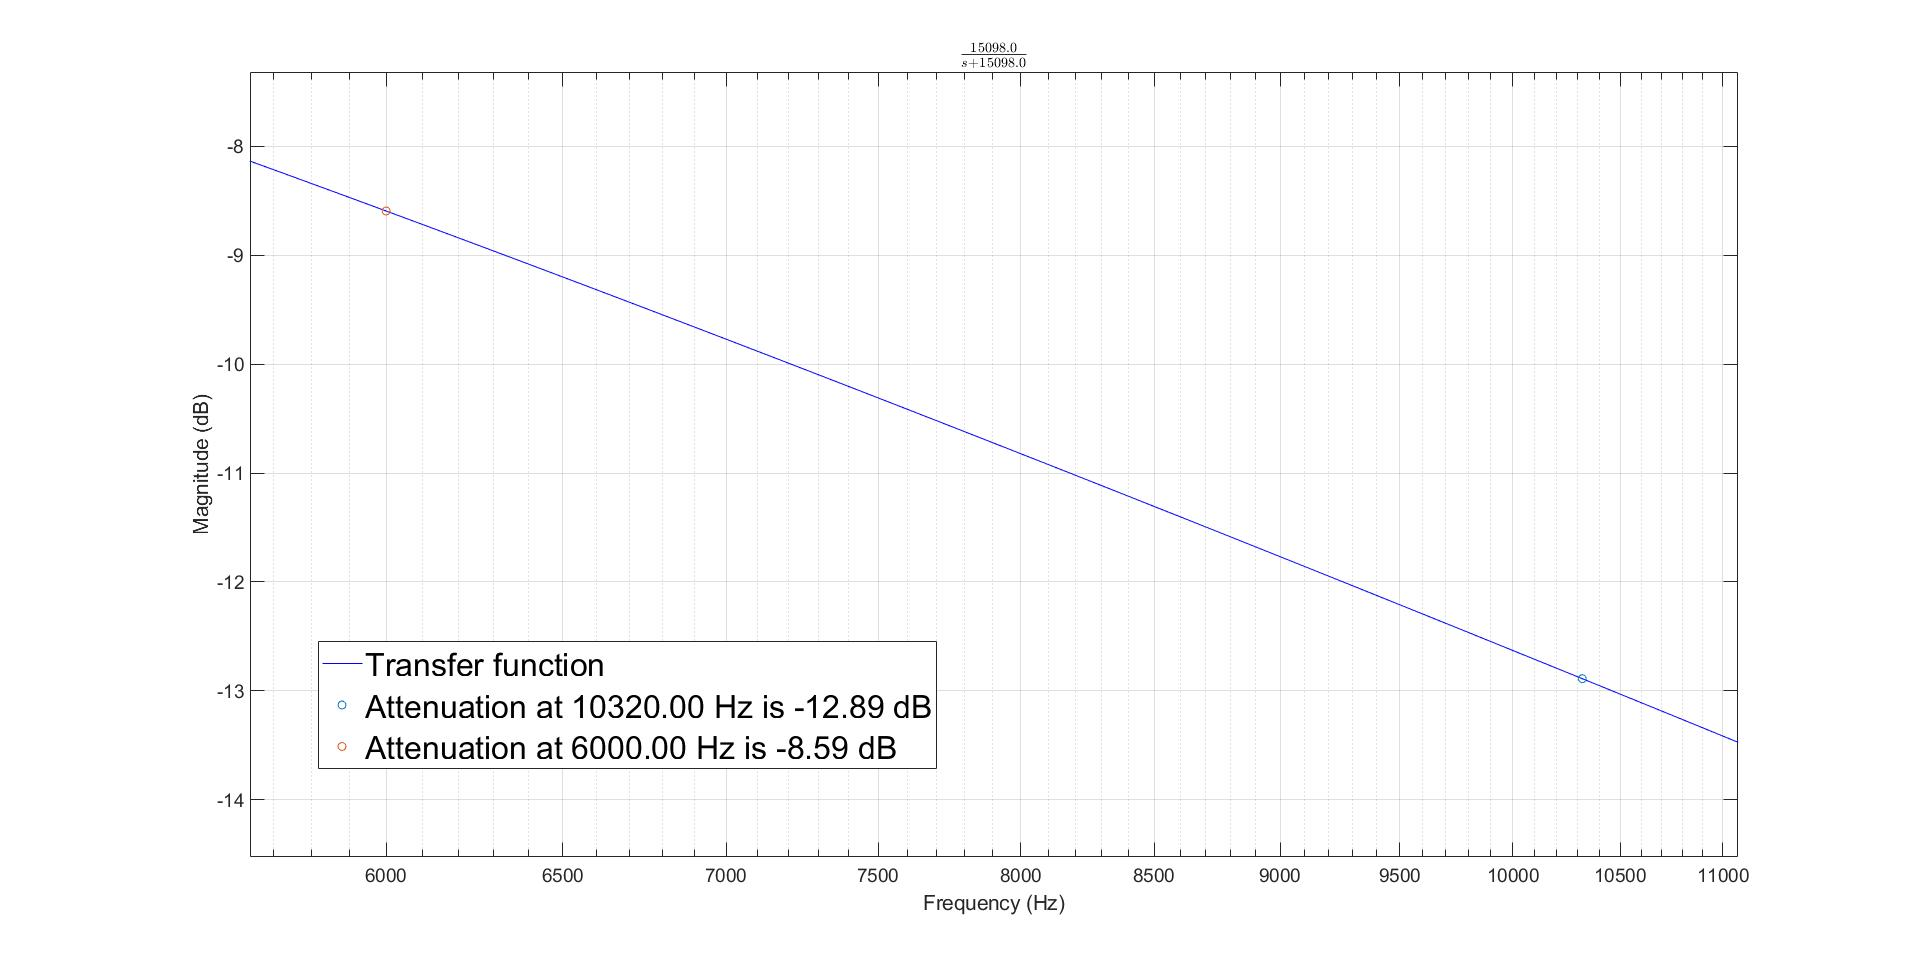
\includegraphics[width=120mm,scale=2]{z1.jpg}
\end{figure*}
\newpage
\section*{$2^\textbf{η}$ Μονάδα : Κύκλωμα Sallen-Key \\ (στρατιγική σχεδίασης 2)} 
  \begin{figure*}[h!]
\centering
 	\advance\leftskip-4cm
  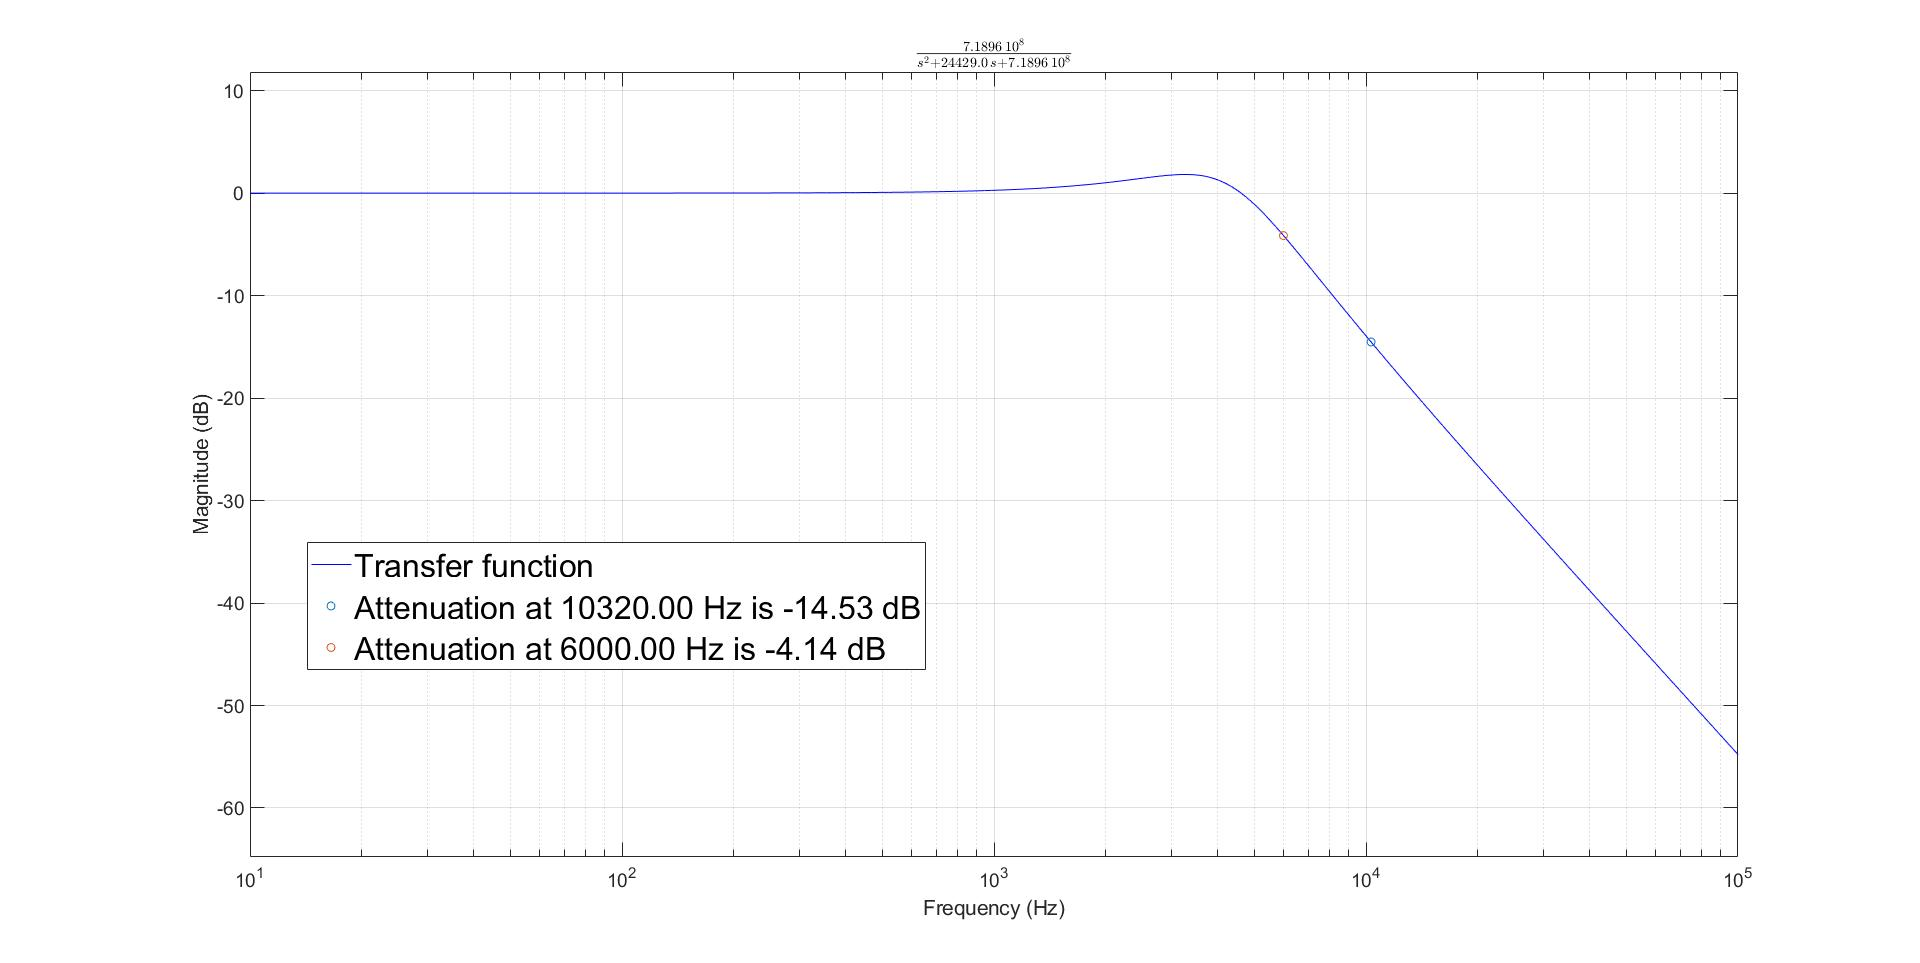
\includegraphics[width=190mm,scale=2]{t2.jpg}
\end{figure*} 
\normalsize{}
Στο παραπάνω διάγραμμα της $2^{ης}$ μονάδας κάνουμε ζουμ ώστε να φαίνεται ευδιάκριτα η απόκριση στις κρίσημες συχνότητες με τις κατάλληλες κλίμακες:
\large{}
 \begin{figure*}[h!]
\centering
 	\advance\leftskip-1cm
  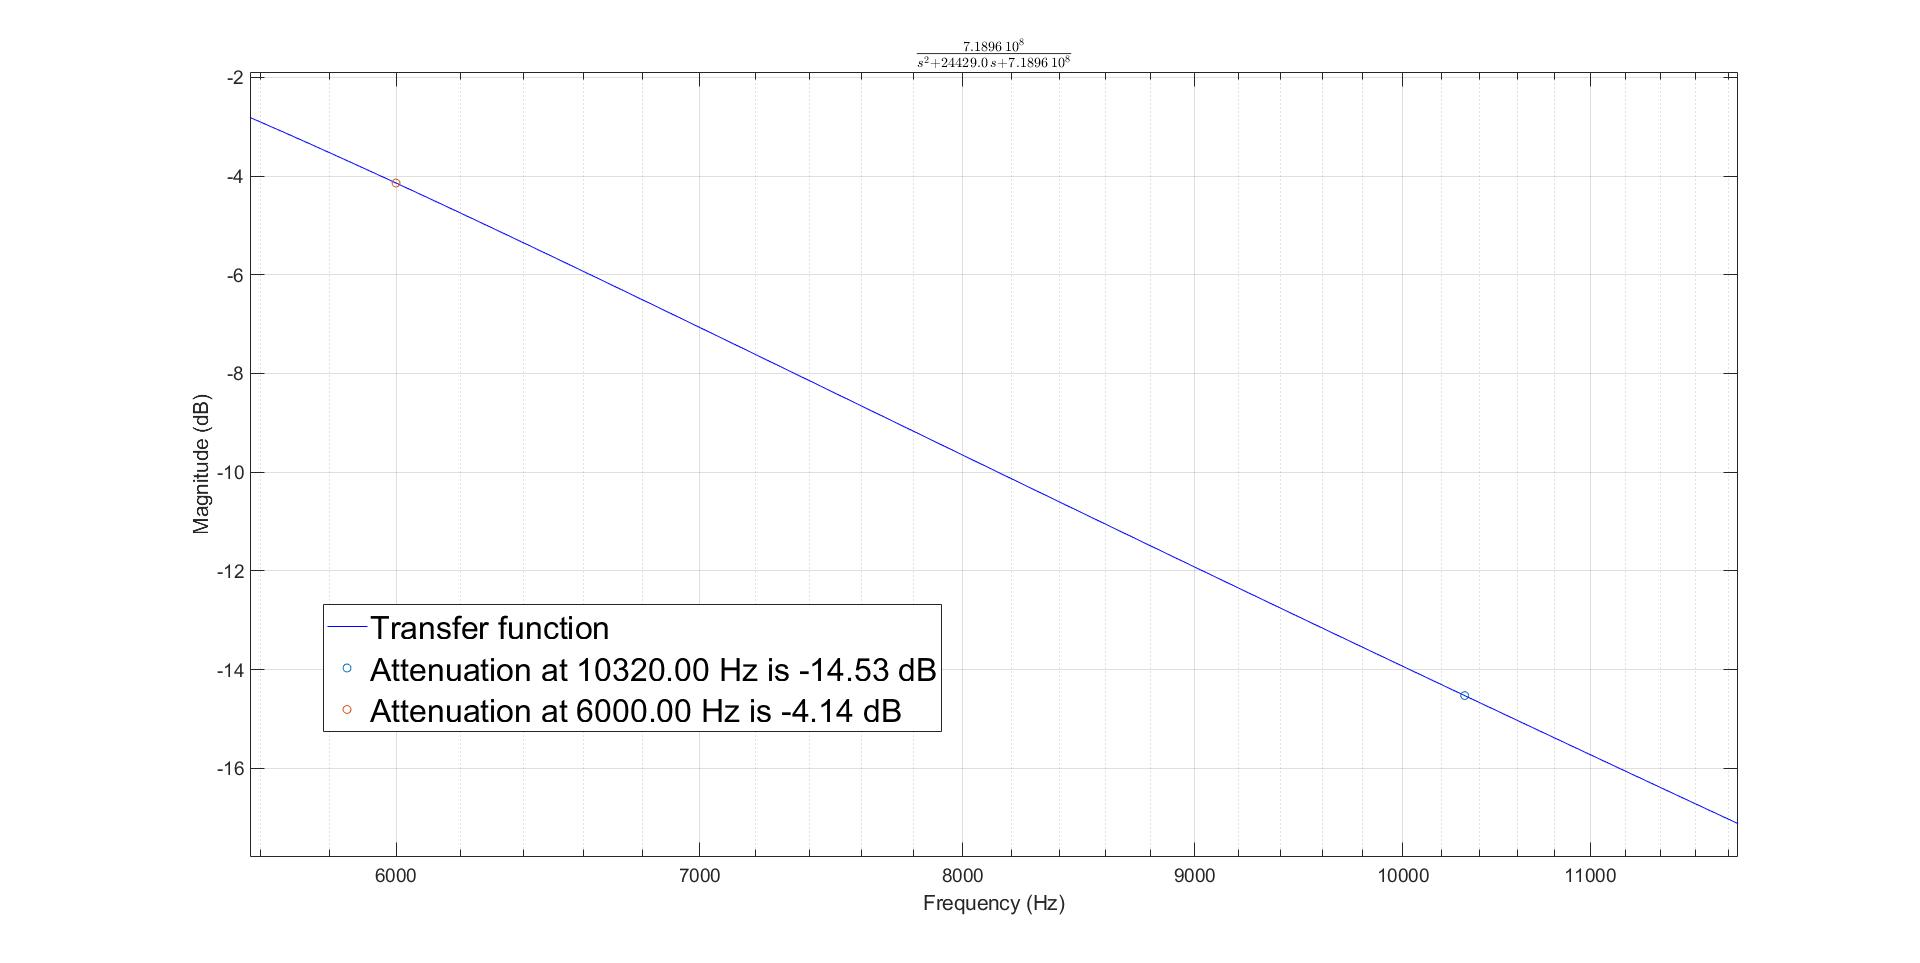
\includegraphics[width=120mm,scale=2]{z2.jpg}
\end{figure*}
\newpage
\section*{$3^\textbf{η}$ Μονάδα : Κύκλωμα Sallen-Key \\ (στρατιγική σχεδίασης 2)} 
  \begin{figure*}[h!]
\centering
 	\advance\leftskip-4cm
  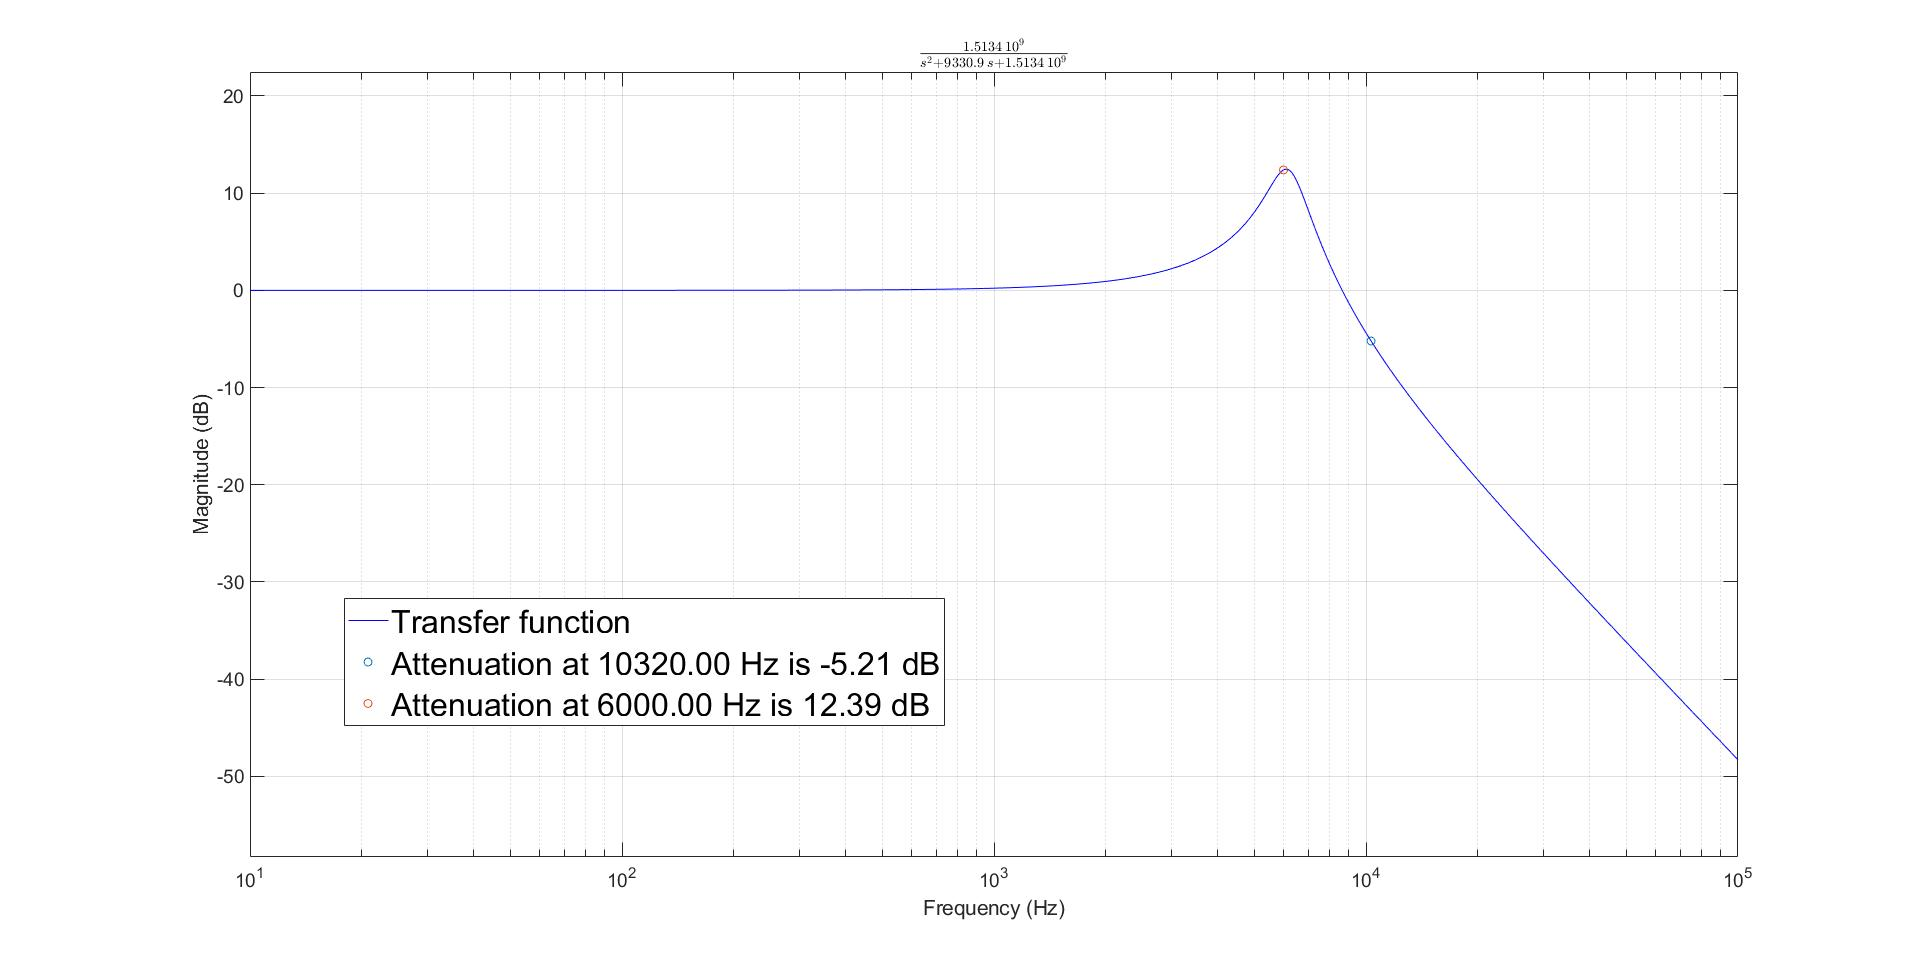
\includegraphics[width=190mm,scale=2]{t3.jpg}
\end{figure*}  
\normalsize{}
Στο παραπάνω διάγραμμα της $3^{ης}$ μονάδας κάνουμε ζουμ ώστε να φαίνεται ευδιάκριτα η απόκριση στις κρίσημες συχνότητες με τις κατάλληλες κλίμακες:
\large{}
 \begin{figure*}[h!]
\centering
 	\advance\leftskip-1cm
  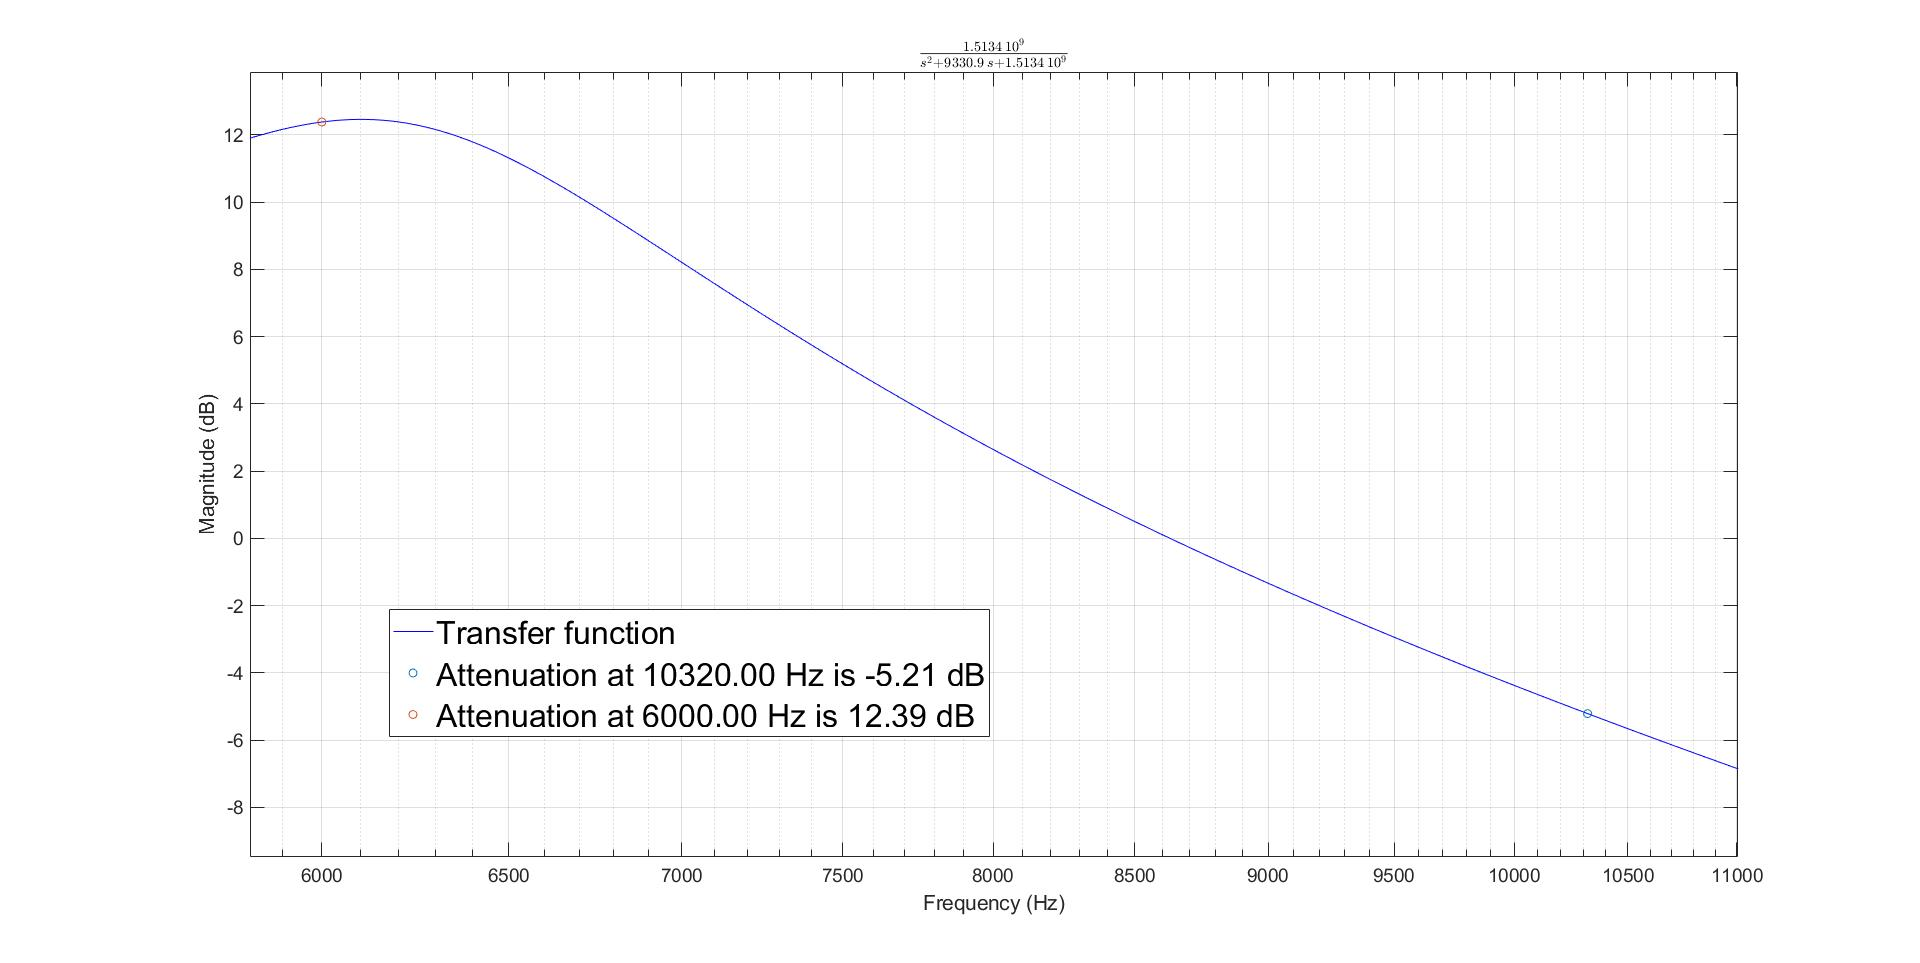
\includegraphics[width=120mm,scale=2]{z3.jpg}
\end{figure*}
\newpage
\section*{Aπόκριση πλάτους της συνολικής συνάρτησης μεταφοράς} 
Παρακάτω βλέπουμε την απόκριση πλάτους της συνολικής συνάρτησης μεταφοράς του φίλτρου συναρτήσει της συχνότητας.
\begin{figure*}[h!]
\centering
 	\advance\leftskip-1cm
  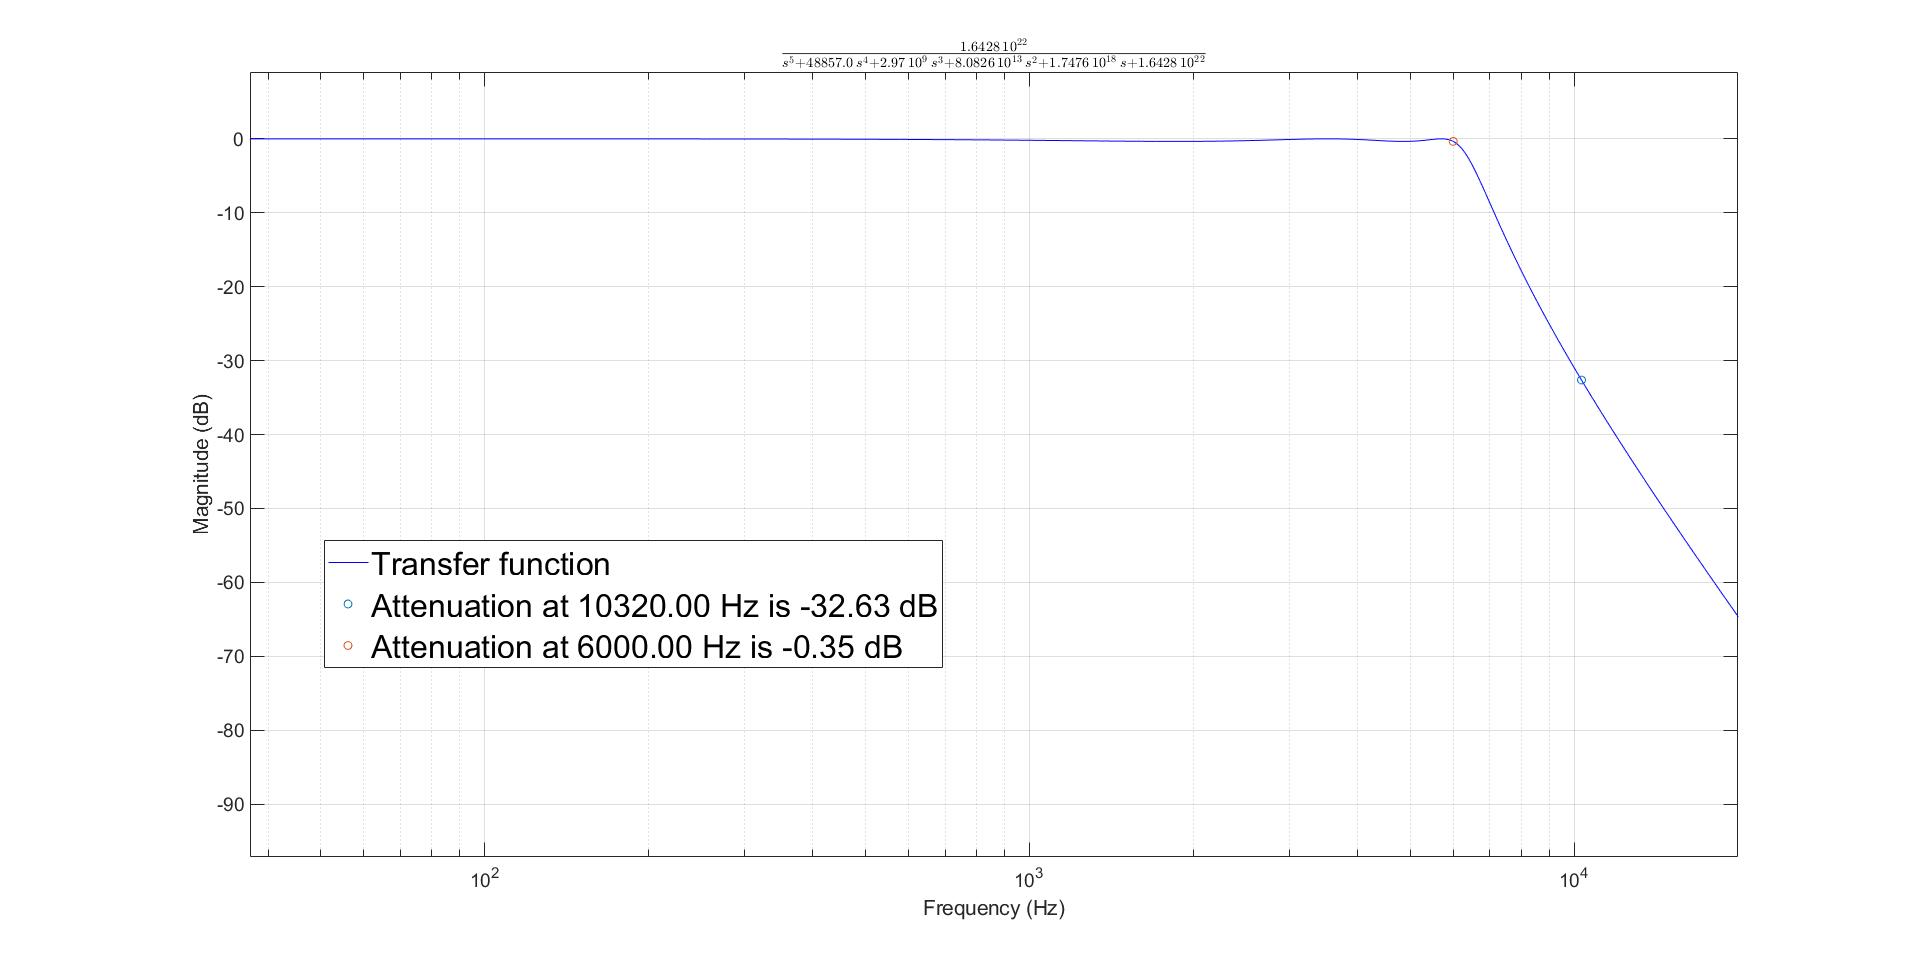
\includegraphics[width=140mm,scale=1]{apokrisi.jpg}
\end{figure*} \\
\normalsize{}
Κάνουμε ζούμ στην ζώνη διόδου και επιλέγουμε κάποια σημεία ώστε να δουμε τις τιμές τους, για τις συχνότητες (0,$f_p$=6000Hz) η απόσβεση δεν ξεπερνά την $a_{max}$ = 0.35dB ενώ για  $f_p=6000Hz$ η απόσβεση είναι ακριβώς όσο το όριο. 
\begin{figure*}[h!]
\centering
 	\advance\leftskip-1cm
  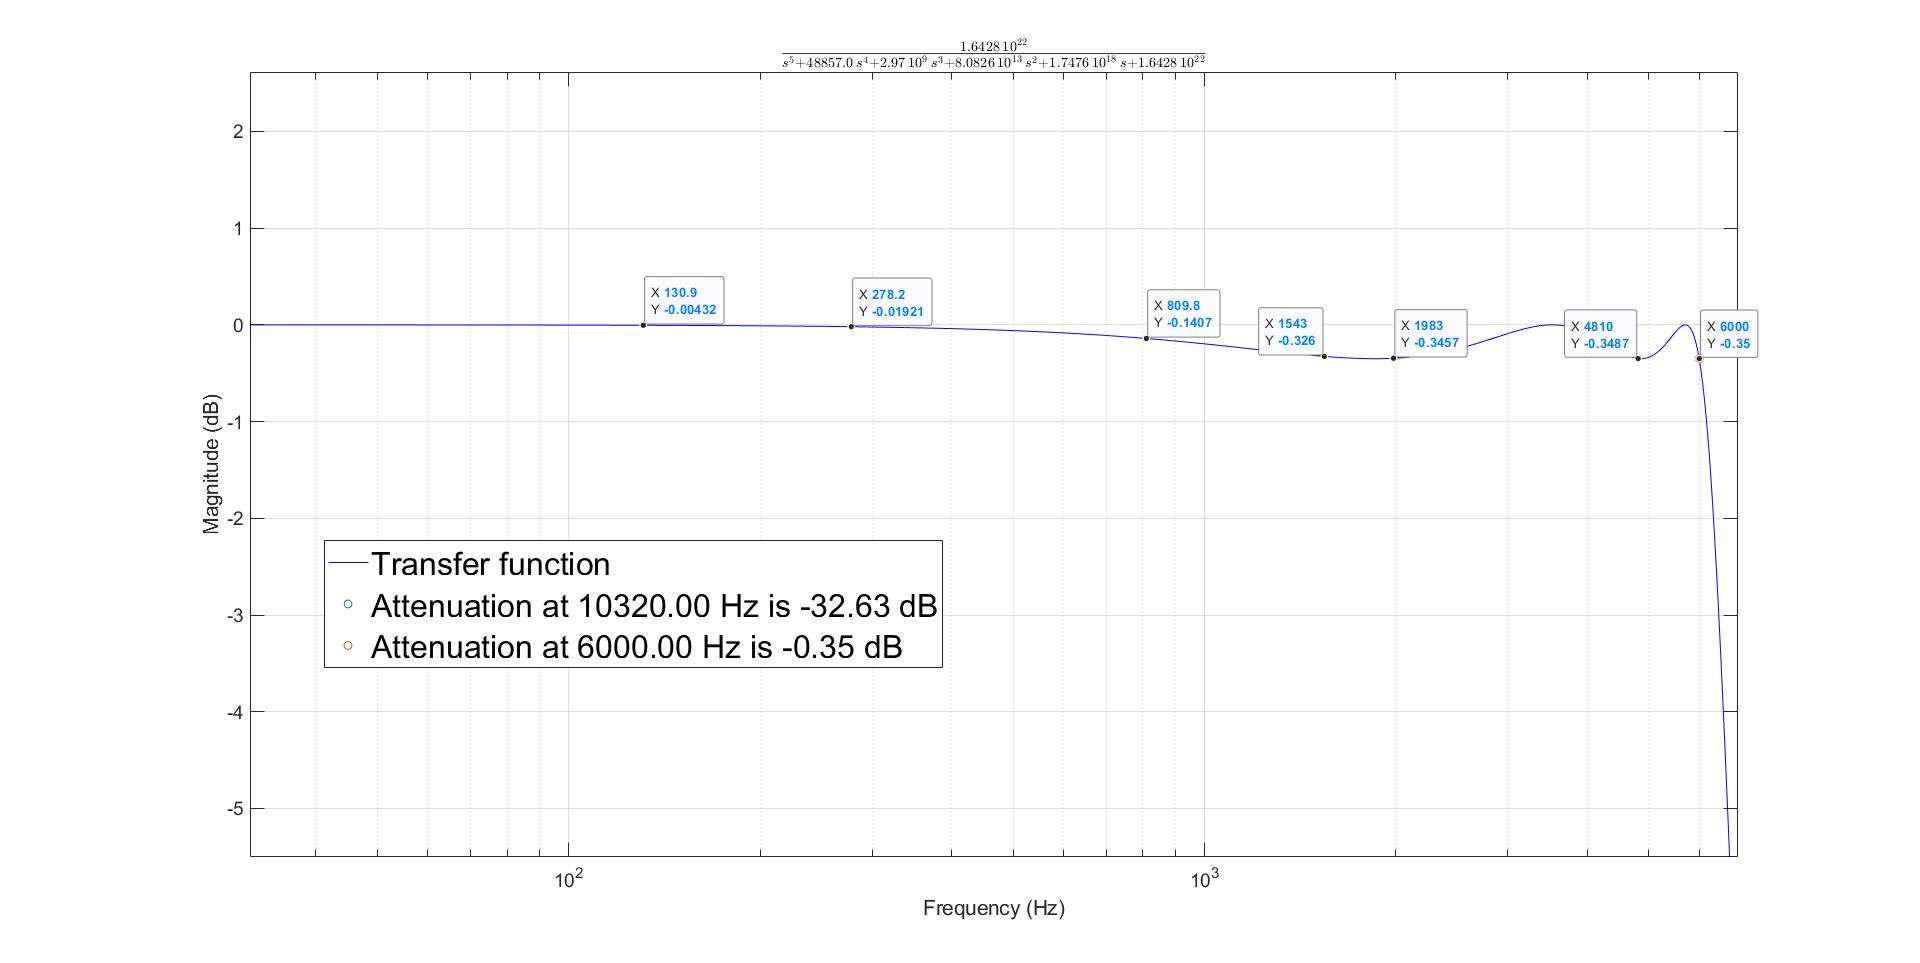
\includegraphics[width=140mm,scale=1]{extra.jpg}
\end{figure*}
\newpage
\section*{Κοινό διάγραμμα αποκρίσεων} 
\large{}
Σε αυτό το σημείο παραθέτουμε όλες τις παραπάνω αποκρίσεις σε ένα κοινό διάγραμμα Bode.
\begin{figure*}[h!]
\centering
 	\advance\leftskip-5cm
  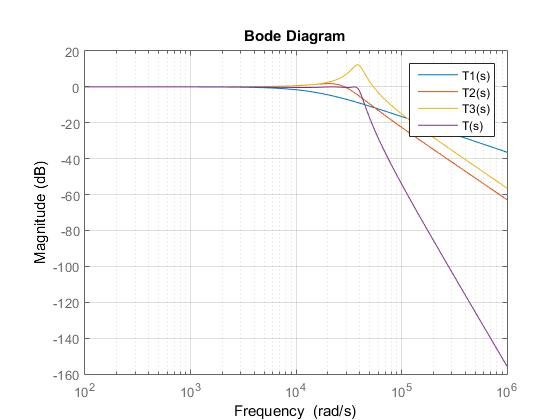
\includegraphics[width=220mm,scale=2]{t_all.jpg}
\end{figure*} 
\newpage
\section*{Συνάρτηση απόσβεσης της συνολικής συνάρτησης μεταφοράς} 
Παρακάτω φαίνεται η συνάρτηση απόσβεσης σε dB της συνολικής συνάρτησης μεταφοράς συναρτήσει της συχνότητας. 
\begin{figure*}[h!]
\centering
 	\advance\leftskip-3cm
  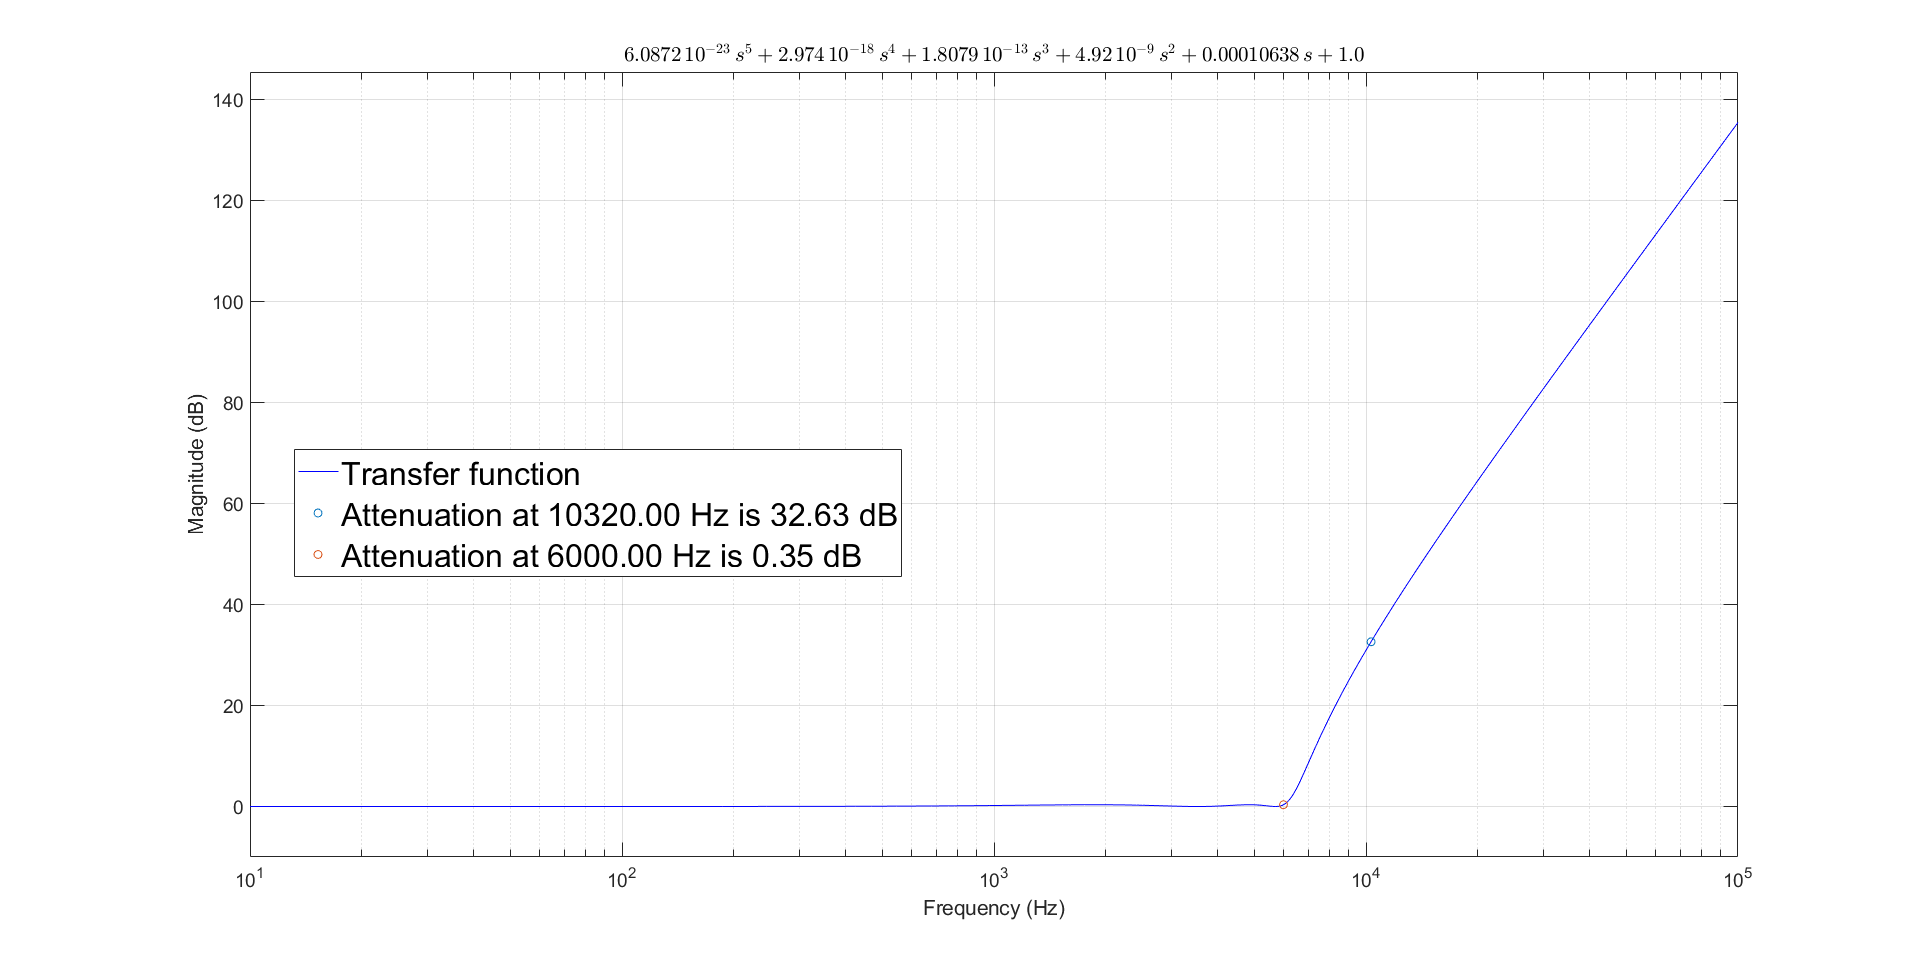
\includegraphics[width=180mm,scale=2]{aposvesi.png}
\end{figure*}  \color{white}{
Στη συνάρτηση} \color{black} Στη συνάρτηση  απόσβεσης σημειώνουμε τις κρίσιμες συχνότητες οι οποίες καθορίζουν την ζώνη διόδου και αποκοπής , δηλαδή την $f_p$=6kHz και την $f_s$=10.32kHz, καθώς και τις αντίστοιχες αποσβέσεις. Παρατηρούμε ότι η απόκριση αυξάνεται.
Κατά συνέπεια για την συχνότητα $f_p$=6kΚHz η απόσβεση είναι 0.35dB και για $f_s$=10.32kHz η απόσβεση είναι 32.63dB. Στην περίπτωση μας επειδη οι μονάδες που επιλέξαμε δινουν κέρδος μονάδα στο dc δεν απαιτείται περαιτέρο διόρθωση του κέρδους ώστε να έχουμε 0dB. Είναι φανερό  λοιπόν ότι πληρείται η προδιαγραφή αφου στην ζώνη διόδου η απόσβεση δε ξεπερνά την $α_{max}$=0.35dB ενω η δεύτερη προδιαγραφή υπερπληρείται αφού το ζητούμενο είναι να ξεπερνά την $a_{min}$ = 25.5dB\\

\clearpage
\subsection*{Γ. Υλοποίηση του Κυκλώματος του Φίλτρου στο MULTISIM}
\addcontentsline{toc}{subsection}{Γ. Υλοποίηση του Κυκλώματος του Φίλτρου στο MULTISIM}
\large{}
Σχεδιάζουμε το κύκλωμα μας στο ElectronicWorkBench (MULTISIM) προκειμένου να ελέγξουμε αν υλοποιεί την συνολική συνάρτηση μεταφοράς που αναλύθηκε στο προηγούμενο στάδιο της εργασίας αλλά και για να διερευνήσουμε την απόκριση του φίλτρου όταν αυτό διεγείρεται από ένα στοιχειώδες περιοδικό σήμα.
Εισάγουμε λοιπόν όπως απαιτείται τις διάφορες στοιχειώδεις μονάδες του φίλτρου που έχουν σχεδιασθεί στην προηγούμενη φάση της εργασίας στο περιβάλλον MULTISIM και παίρνουμε το παρακάτω κύκλωμα.
\begin{figure*}[h!]
\centering
 	\advance\leftskip-4.3cm
  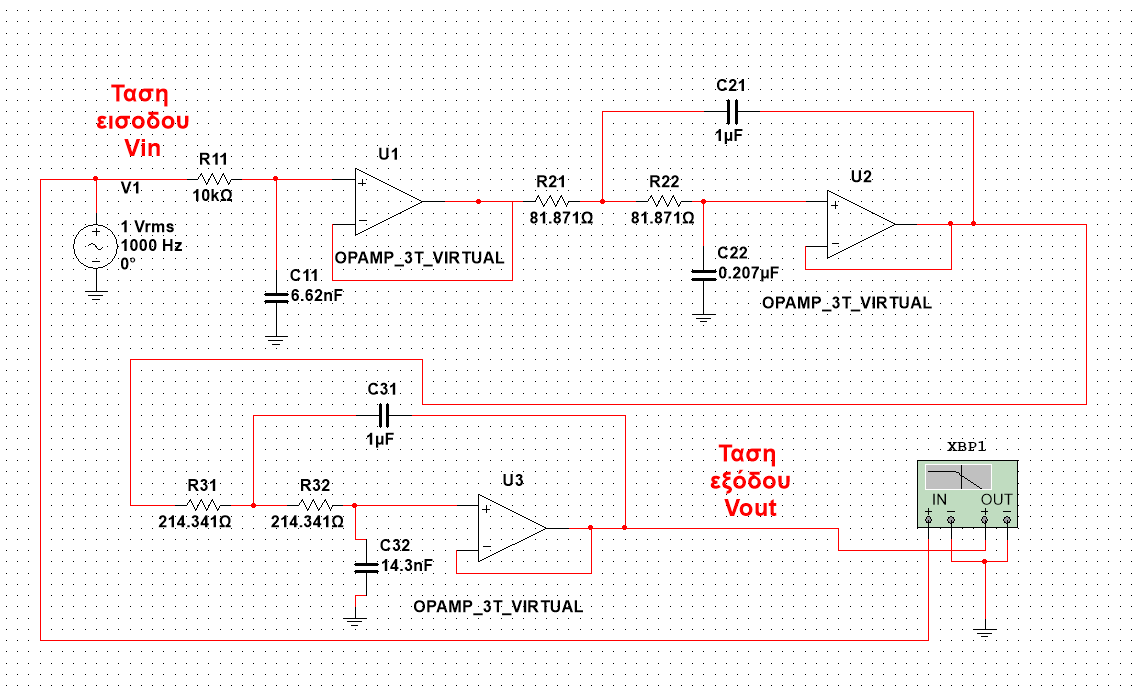
\includegraphics[width=210mm,scale=2]{ylopoiisi.png}
\end{figure*} 
\clearpage
Στο κύκλωμα που έχουμε σχεδιάσει χρησιμοποιούμε τον Bode-Plotter για να προκύψει η απόκριση συχνότητας του φίλτρου-κυκλώματος. Το διάγραμμα που παίρνουμε φαίνεται παρακάτω :
\begin{figure*}[h!]
\centering
 	\advance\leftskip-4cm
  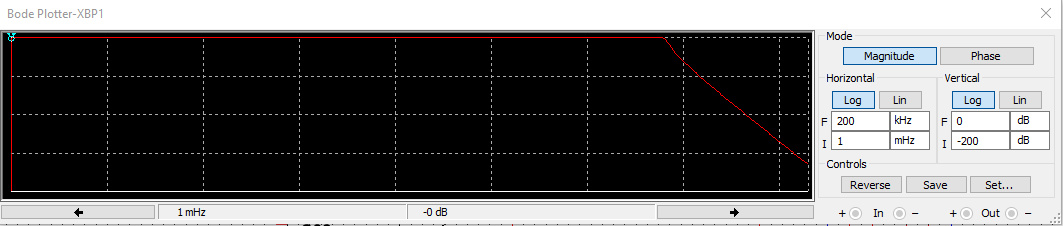
\includegraphics[width=200mm,scale=2]{bode_ploter.png}
\end{figure*} \\
Tο παρακάτω διάγραμμα του Multisim απεικονίζει ότι ακριβώς και το προηγούμενο αλλά με δυνατότητα ανάγνωσης των τιμών $f_p$ και $f_s$.
\begin{figure*}[h!]
\centering
 	\advance\leftskip-4.3cm
  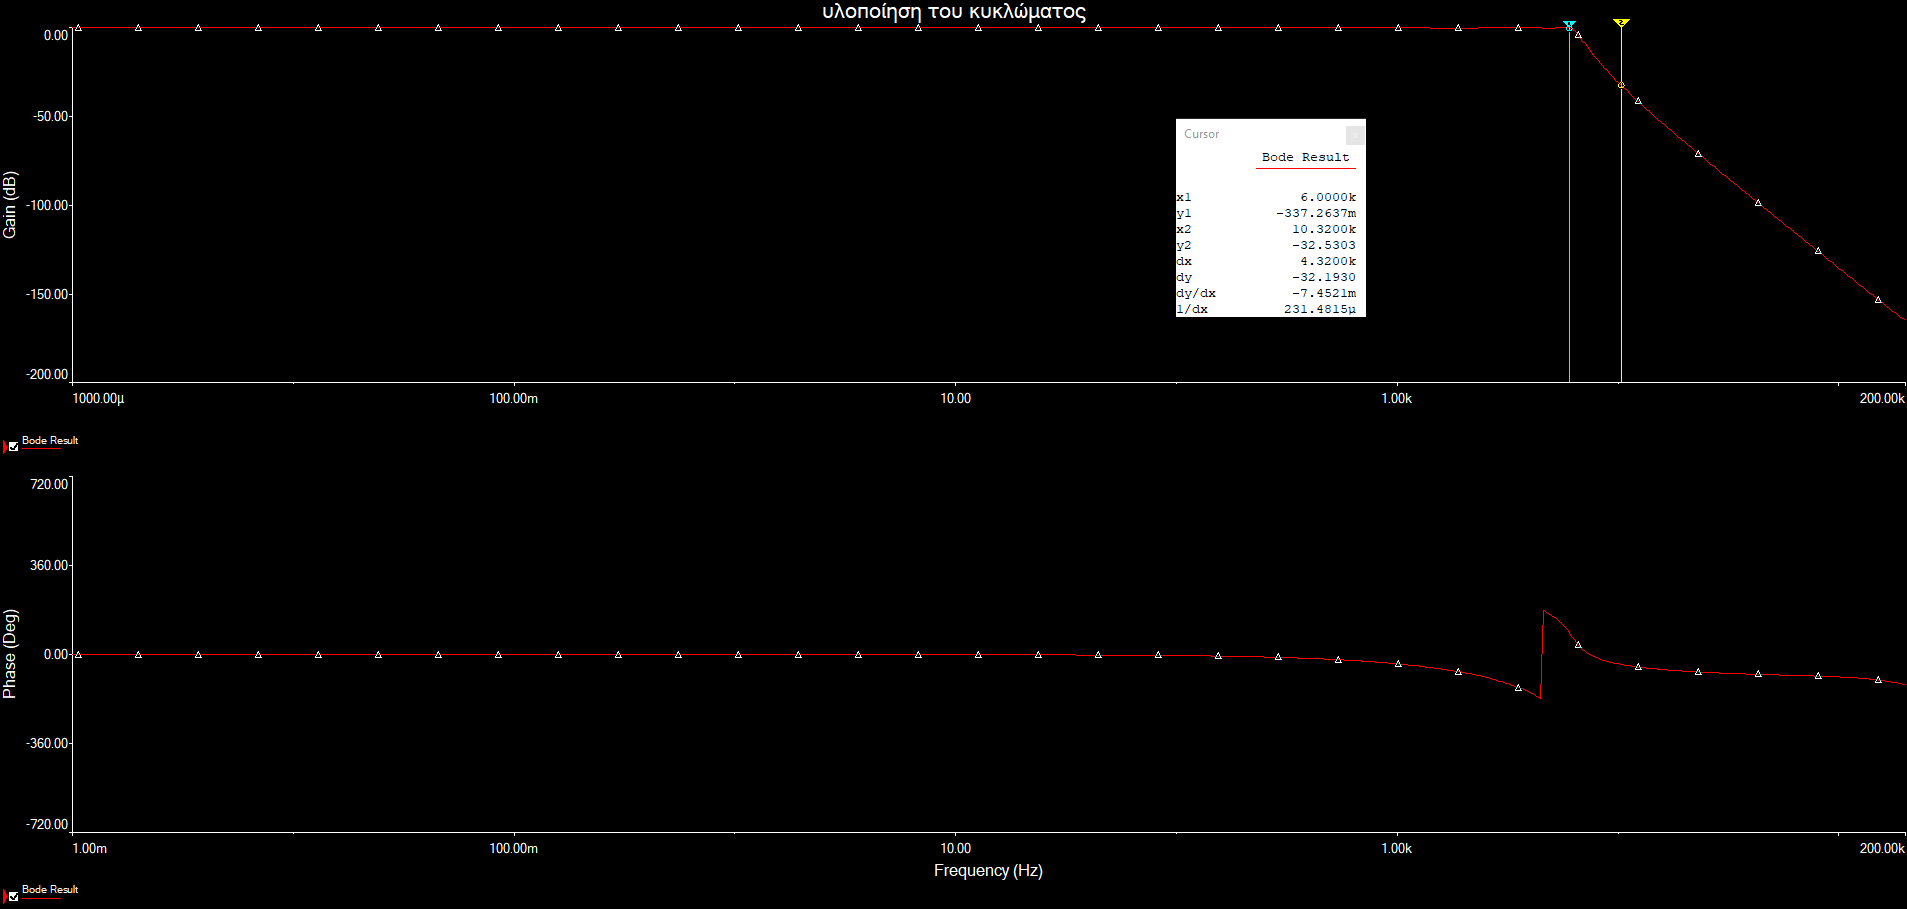
\includegraphics[width=210mm,scale=2]{bode_ploter2.png}
\end{figure*} 
\clearpage
Ελέγχοντας κατάλληλα τις κλίμακες συχνότητας και απόσβεσης διαπιστώνουμε ότι το φίλτρο στις χαμηλές συχνότητες έχει κέρδος 0dB οπως και απαιτείται \\
\begin{figure*}[h!]
\centering
 	\advance\leftskip-4.4cm
  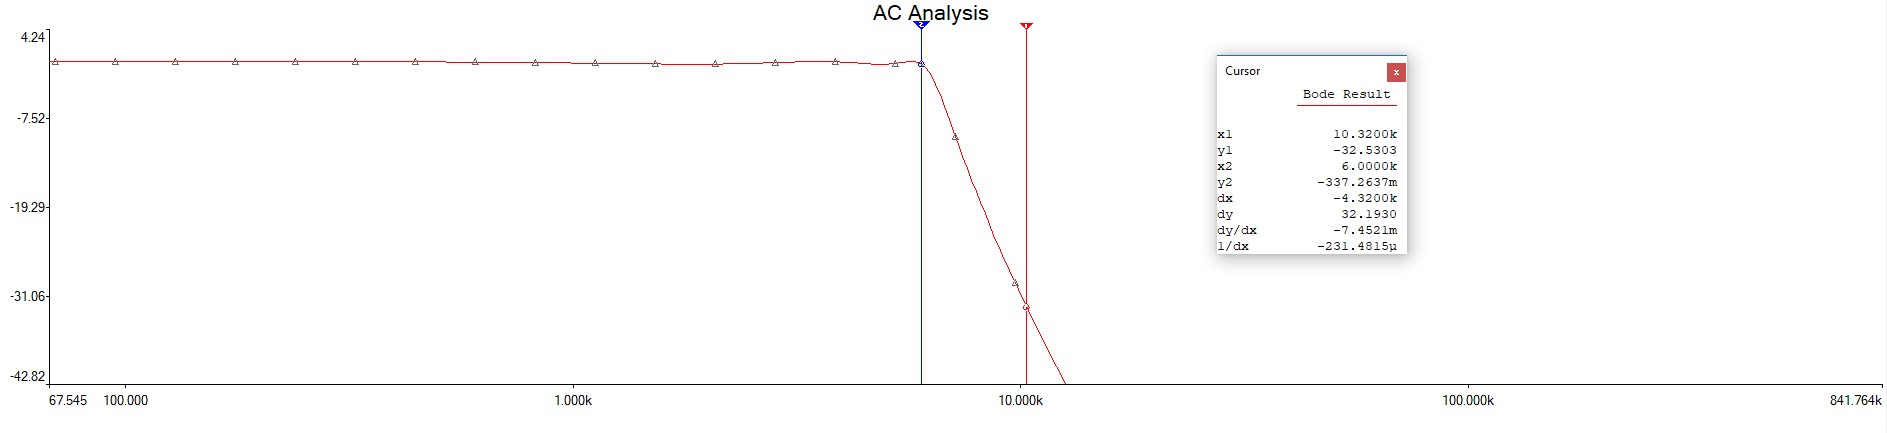
\includegraphics[width=215mm,scale=2]{ac1.jpg}
\end{figure*} \\
Απο τα διαγράμματα που ακολούθησαν είναι φανερό ότι πληρείται η προδιαγραφή της  $α_{max}$ καθώς στην ζώνη διόδου η απόσβεση δε ξεπερνά την $α_{max}$=0.35dB. Βλέπουμε οτι για $f_p$ = 6kHz η απόσβεση είναι 0.337 dB \\ Η δεύτερη προδιαγραφή υπερπληρείται επειδή για την συχνότητα $f_s$=10.32kHz η απόσβεση είναι 32.53dB  που ξεπερνά το ζητούμενο δηλαδή την $a_{min}$ = 25.5dB \\
Συνεπώς η ζώνη αποκοπής εχει αρκετα καλη απόσβεση  
\clearpage
Εισάγουμε τώρα στο κύκλωμα με μια πηγή διέγερσης πριονοτού σήματος με θεμελιώδη συχνότητα 2kHz . Στην συνέχεια χρησιμοποιούμε έναν παλμογράφο στην είσοδο και την έξοδο και δημιουργούμε τα αντίστοιχα figures για το παραπάνω πείραμα.
\begin{figure*}[h!]
\centering
 	\advance\leftskip-4cm
  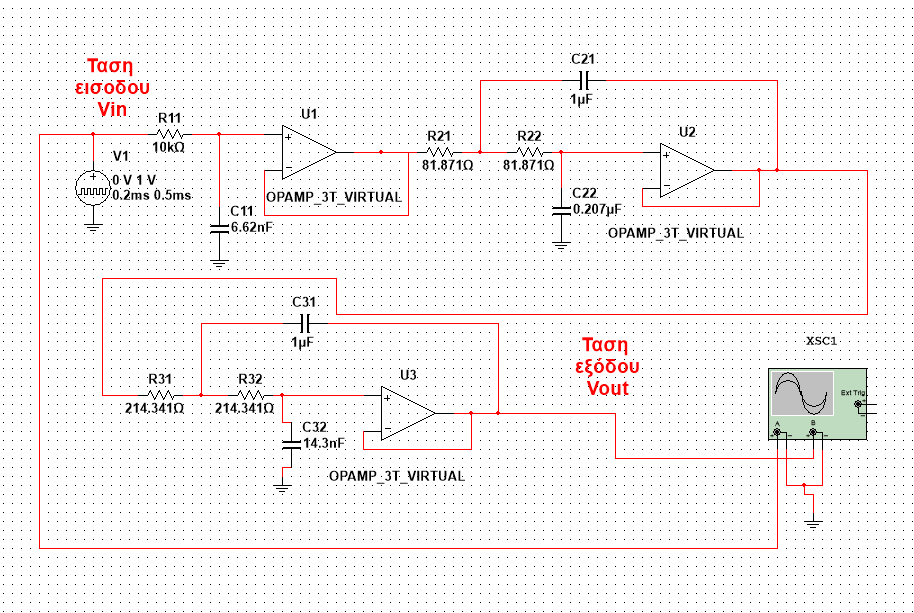
\includegraphics[width=200mm,scale=2]{circ.png}
\end{figure*} 
\\
Στα διαγράμματα που θα ακολουθήσουν θα αναπαραστήσουμε τα σήματα εισόδου με χρώμα μπλε και τα σήματα εξόδου με χρώμα πρασινο.
\clearpage
\textbf{\underline{Σήμα Εισόδου (Εικόνα παλμογράφου):}}
\begin{figure*}[h!]
\centering
 	\advance\leftskip-3cm
  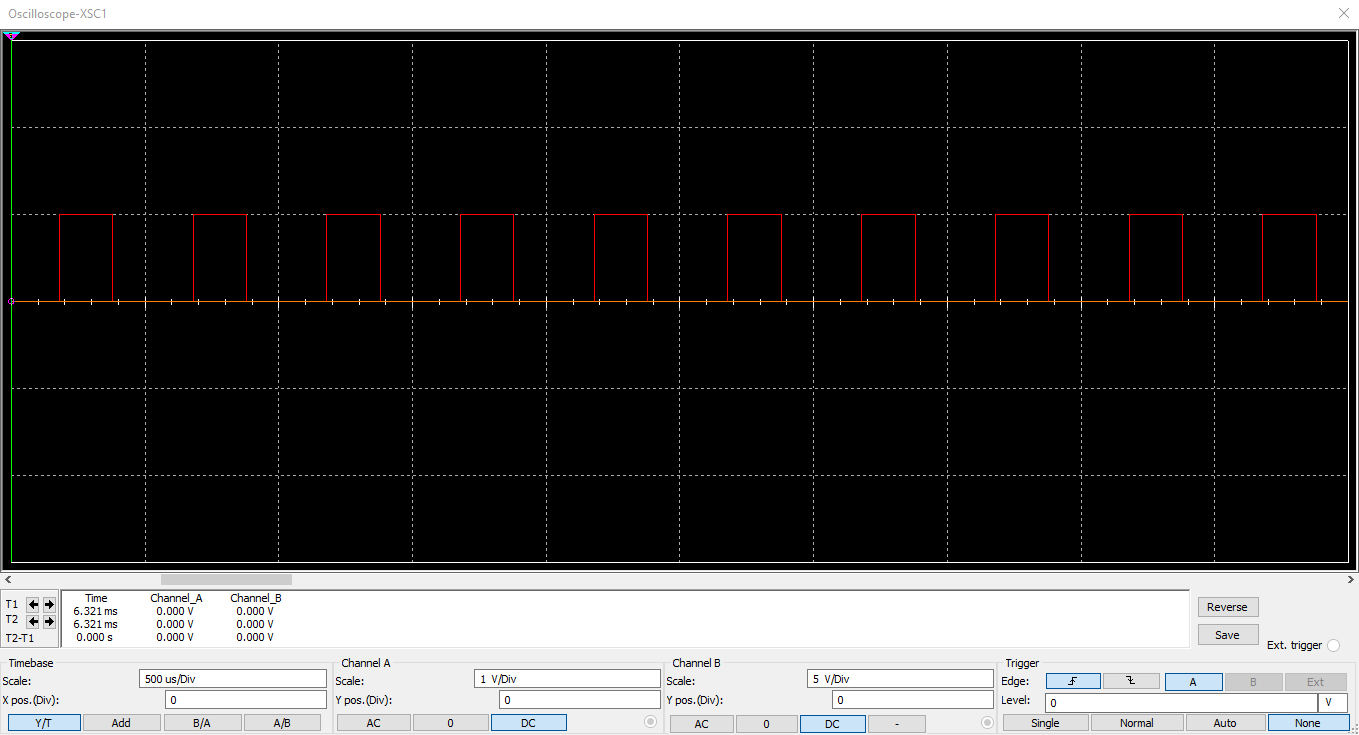
\includegraphics[width=180mm,scale=2]{input.png}
\end{figure*} \\
\textbf{\underline{Transient Analysis σηματος ειδόσου (με ασπρο φόντο):}}
\begin{figure*}[h!]
\centering
 	\advance\leftskip-2cm
  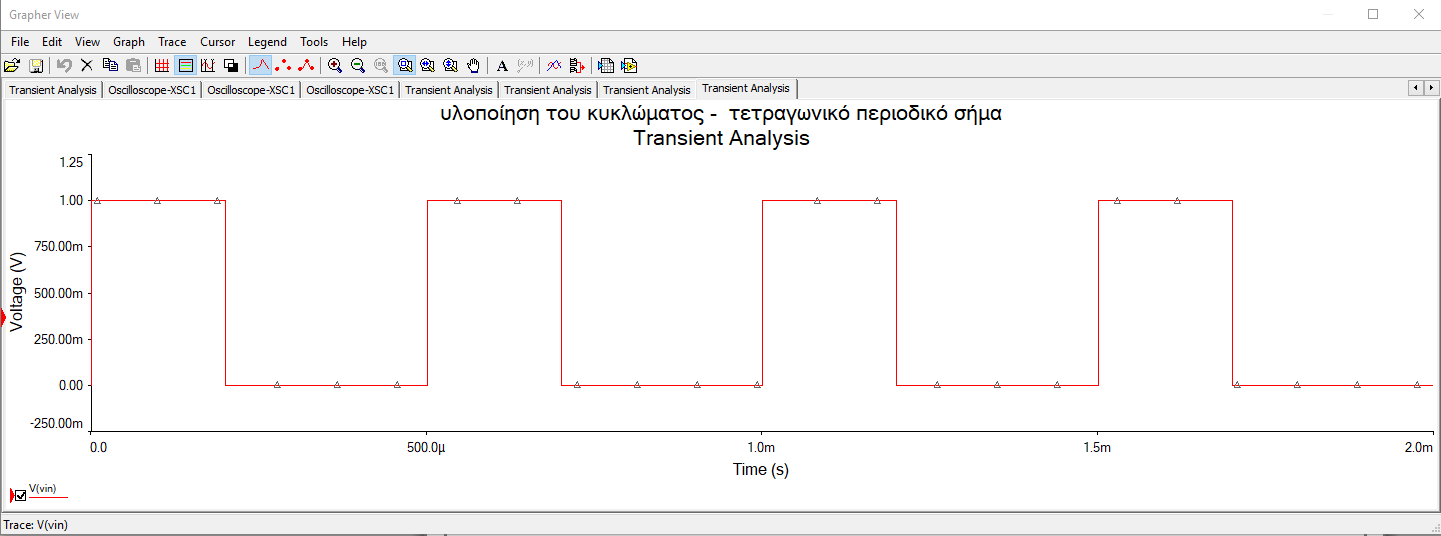
\includegraphics[width=160mm,scale=2]{input2.png}
\end{figure*} 
\clearpage
\textbf{\underline{Σήμα Εξόδου (Εικόνα παλμογράφου):}}
\begin{figure*}[h!]
\centering
 	\advance\leftskip-3cm
  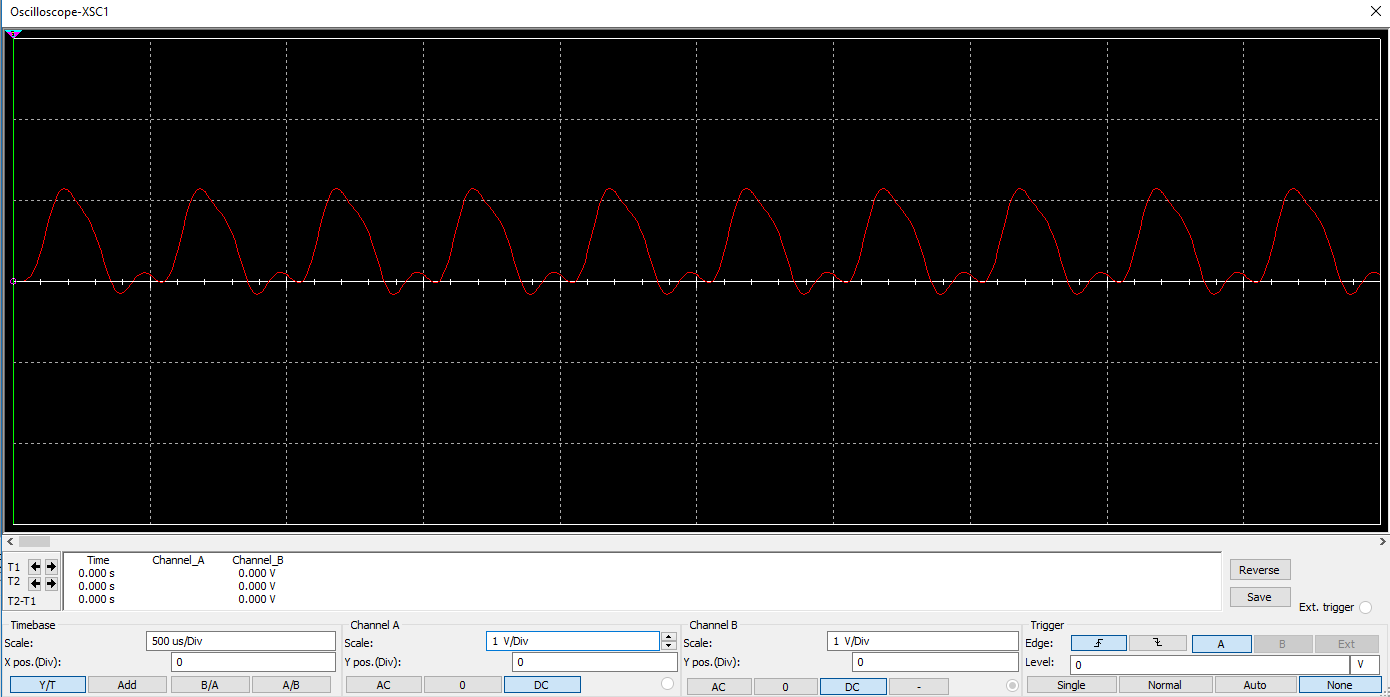
\includegraphics[width=180mm,scale=2]{output.png}
\end{figure*} \\
\textbf{\underline{Transient Analysis σηματος εξόδου (με ασπρο φόντο):}}
\begin{figure*}[h!]
\centering
 	\advance\leftskip-3cm
  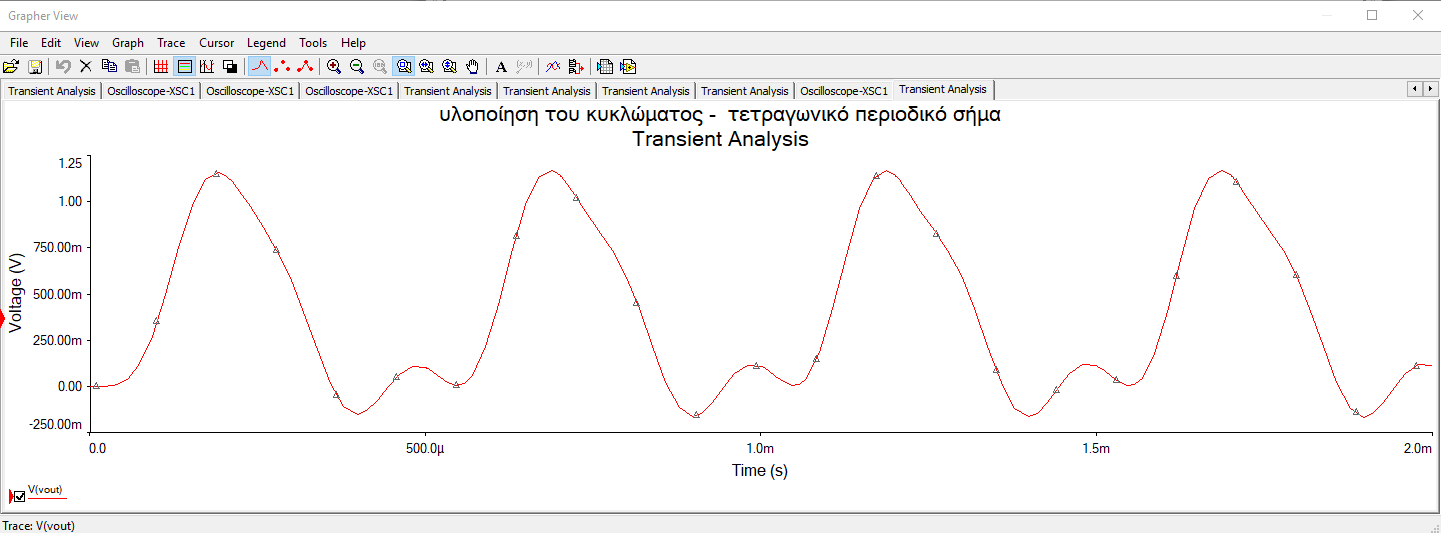
\includegraphics[width=180mm,scale=2]{output2.png}
\end{figure*} 
 \clearpage
 \textbf{\underline{Σήμα Εισόδου-Εξόδου (Εικόνα παλμογράφου):}} 
 \\[1.4\baselineskip]
 Το διάγραμμα που ακολουθεί περιλαμβάνει \textcolor{blue}{το σήμα ειδόδου (μπλέ χρώμα)} και \textcolor{green}{το σήμα εξόδου (πράσινο χρωμα)} στα channel του παλμογράφου Α και Β αντίστοιχα.  \\[0.4\baselineskip]
 \begin{figure*}[h!]
\centering
 	\advance\leftskip-2.8cm
  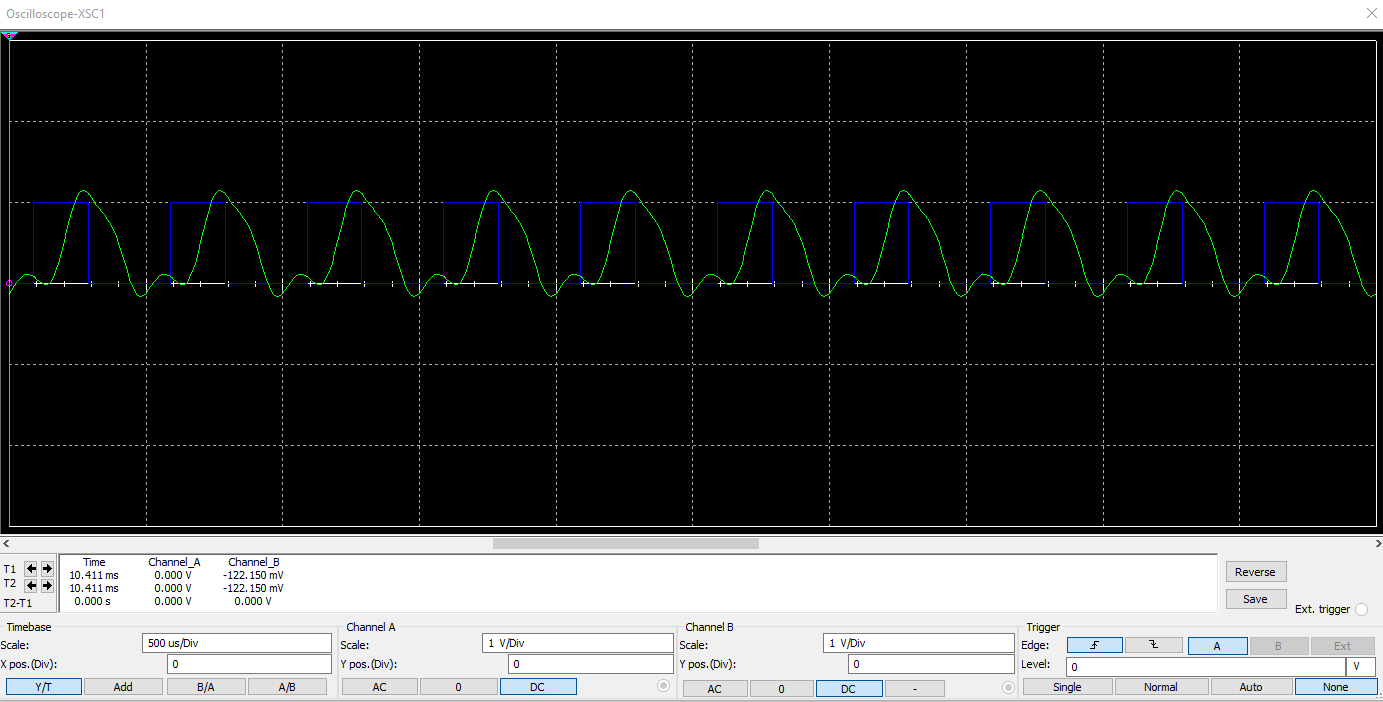
\includegraphics[width=180mm,scale=2]{input-output.png}
\end{figure*}   \\[1.4\baselineskip]
Στα παραπάνω διαγράμματα μπορούμε να δούμε αναλυτικά \textcolor{blue}{τα σήματα εισόδου (channel a)} και \textcolor{green}{εξόδου (channel b)} σε κάθε σχήμα φαίνονται οι επιλογές που κάναμε στον παλμογράφο για να προκύψουν οι αντίστοιχες παραστάσεις (για παράδειγμα: V/Div ,  sec/Div κτλ.).
Πιο αναλυτικά, παρατηρούμε ότι το σήμα εξόδου είναι ίσο σε πλάτος σε σχέση με το σήμα εισόδου. Το κέρδος του φίλτρου γίνεται φανερό, καθώς το σήμα εξόδου εχει 0dB ενίσχυση. Επειδή το χαμηλοπερατό φίλτρο αποσβένει στις συχνότητες πέρα από f $>$ fs = 10.32kHz, παραμένουν μια DC συνιστώσα και κάποιες αρμονικές, που είναι πολλαπλάσια της θεμελιώδους αρμονικής $f_0$ = 2 kHz. Αυτό υποδηλώνεται και απ το γενονός οτι η έξοδος έχει μία ημιτονοειδή μορφή.
\clearpage
\subsection*{Σύκριση matlab-multisim}
\large{}
Σε αυτό το σημείο της άσκησης θέλουμε να δημιουργήσουμε τα φάσματα εισόδου και εξόδου του φίλτρου, Chebyshev. Για να γίνει κάτι τέτοιο θα εξετάσουμε τα φάσματα τόσο στο Multisim όσο και στο Matlab. Εφόσον μιλάμε για τα ίδια σήματα καθώς και για το ίδιο φίλτρο, αναμένουμε να έχουμε τα ίδια αποτελέσματα. \\[0.4\baselineskip]
Κατά συνέπεια, στην επόμενη σελίδα παρουσιάζουμε τα φάσματα FOURIER που προέρχονται από την FFT και τα οποία θα σχολιάσουμε στην συνέχεια.\\[1.8\baselineskip]
\subsection*{Σχολιασμός}
Στα παραπάτω διαγράμματα του multisim και του matlab φαίνεται ότι οι αρμονικές που βρίσκονται εντός της ζώνης διόδου, δηλαδή έχουν συχνότητα f $<$ fp = 6 kHz, δεν μεταβάλλονται κάτι το οποίο είναι απολύτως λογικό εφόσον το κύκλωμα μας είναι ένα lowpass φιλτρο. Οι κρίσιμες συχνότητες για το συγκεκριμένο φίλτρο είναι fp=6kHz και fs=10.32kHz . Οι αρμονικές που βρίσκονται στην ζώνη αποκοπής, δηλαδή αυτές που έχουν συχνότητα f $>$ fs = 10.32 kHz, αποσβένυνται, δηλαδή αποκόπτονται από το φίλτρο. Στο ενδιάμεσο αυτών των περιοχών, δηλαδή για fp $<$ f $<$ fs, οι
αντίστοιχες αρμονικές υφίστανται μία απόσβεση, όχι όμως τόσο σημαντική
όσο στην περίπτωση που βρισκόμαστε στην περιοχή αποκοπής.



\clearpage
\textbf{\underline{Σήμα Εισόδου (Fourier) - MATLAB:}}
\begin{figure*}[h!]
\centering
 	\advance\leftskip-2.2cm
  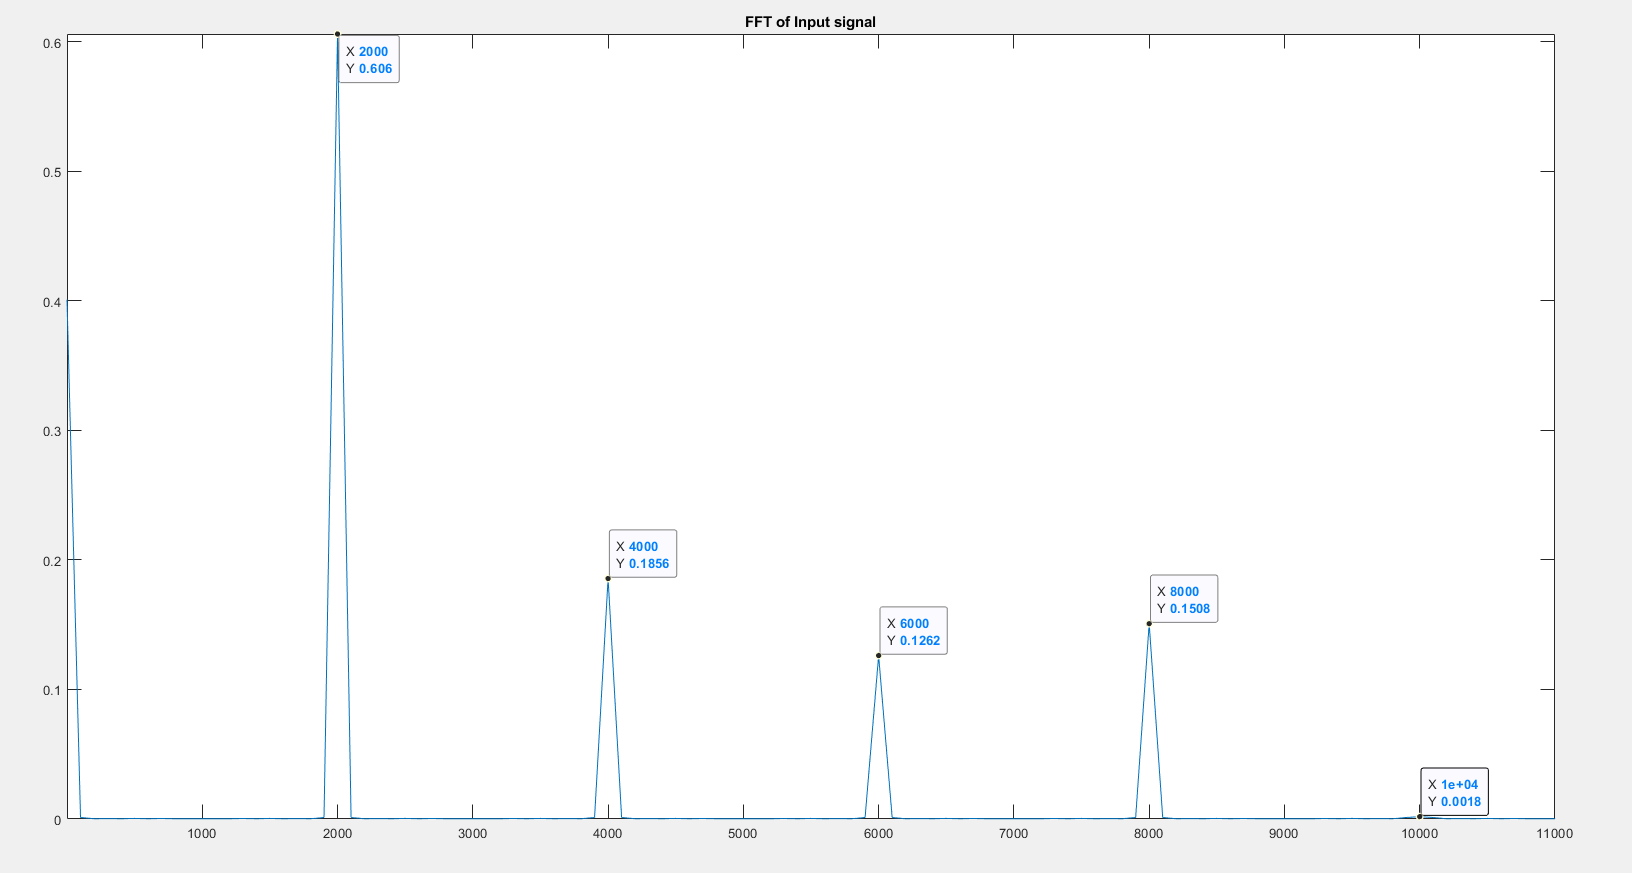
\includegraphics[width=150mm,scale=2]{multisim8_input.png}
\end{figure*} \\[1.4\baselineskip]
\textbf{\underline{Σήμα Εξόδου (Fourier) - MATLAB:}}
\begin{figure*}[h!]
\centering
 	\advance\leftskip-2.2cm
  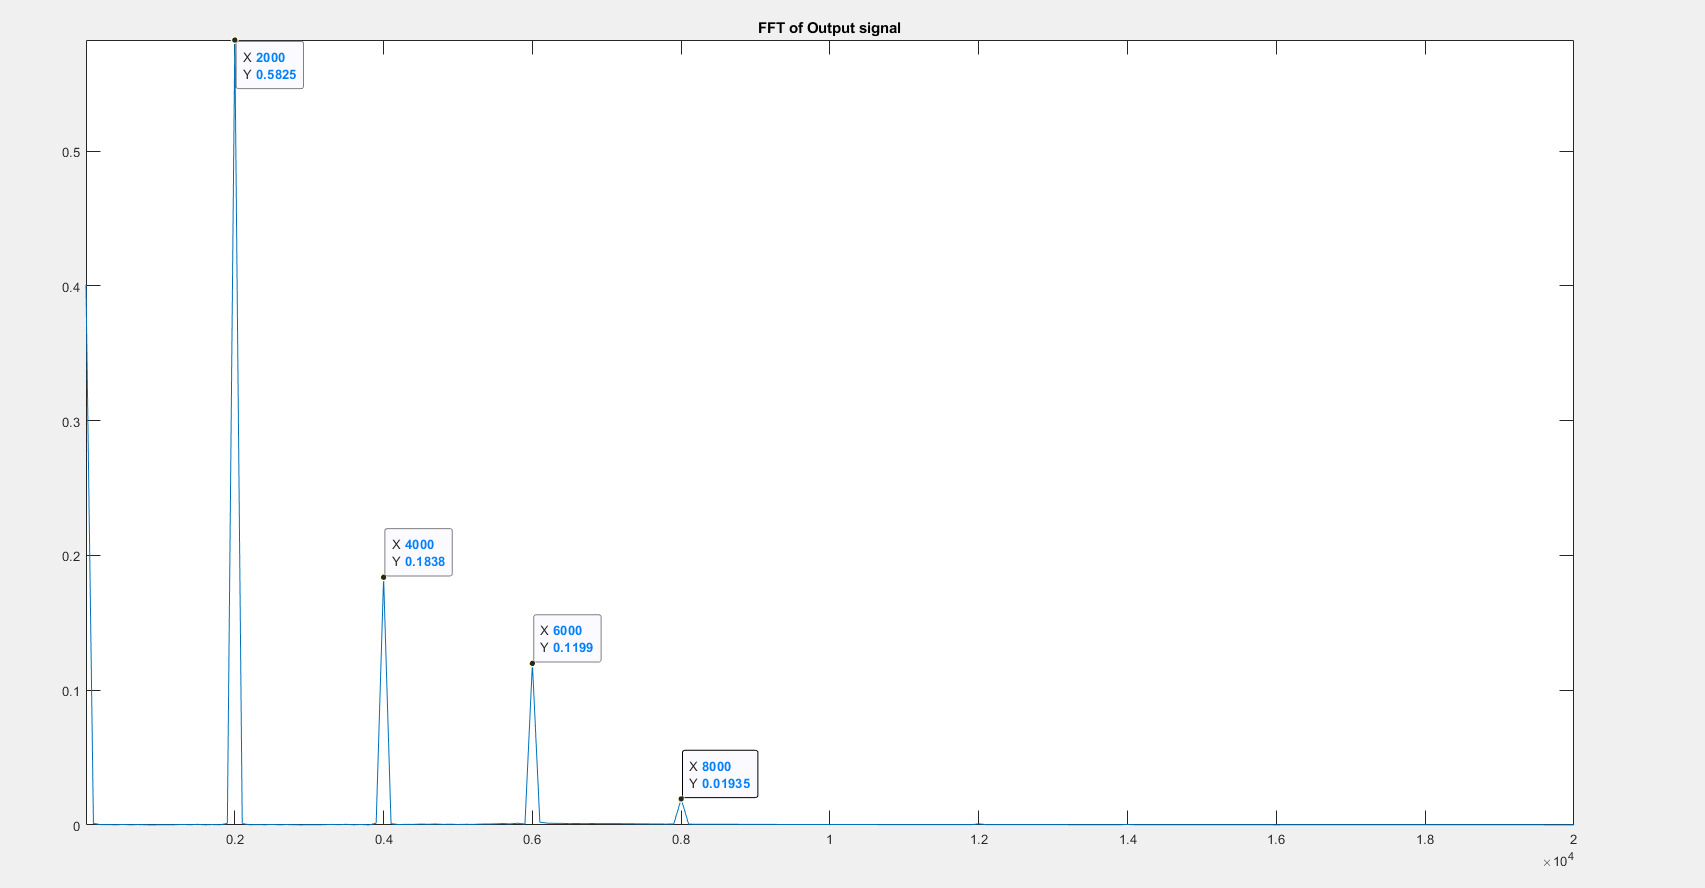
\includegraphics[width=150mm,scale=2]{multisim9_output.png}
\end{figure*} 
\clearpage
\textbf{\underline{Σήμα Εισόδου (Fourier) - MULTISIM:}}
\begin{figure*}[h!]
\centering
 	\advance\leftskip-2cm
  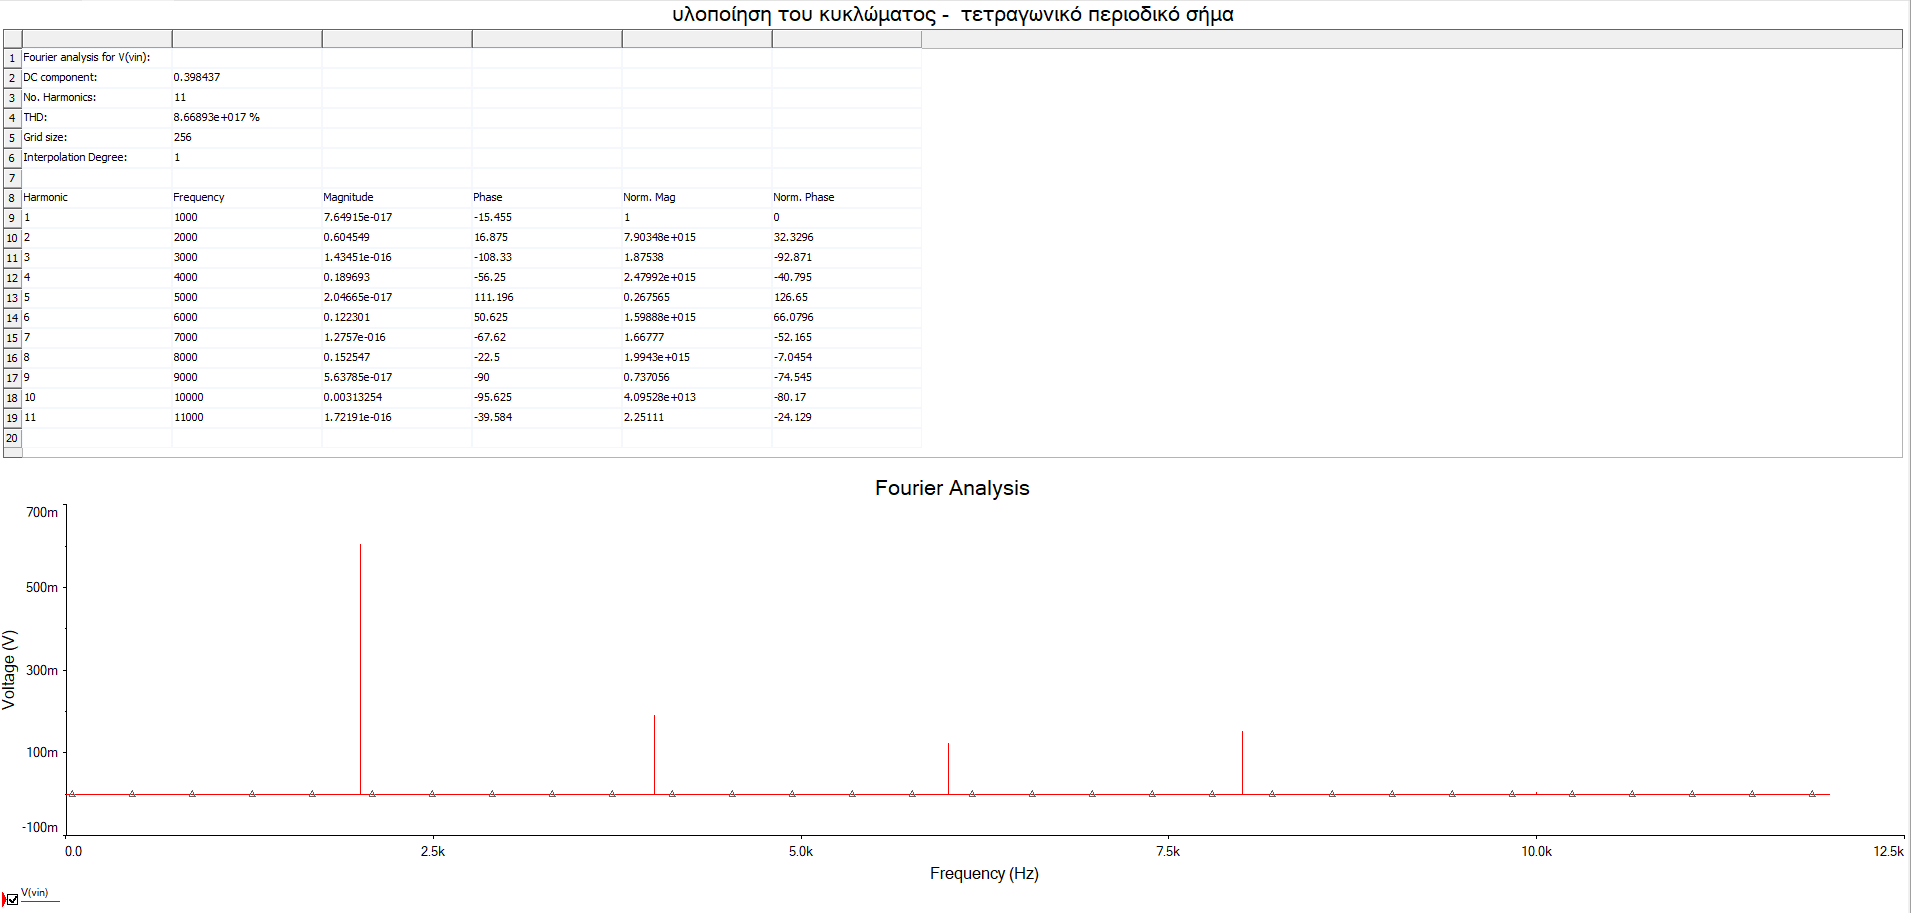
\includegraphics[width=160mm,scale=2]{multisim9.png}
\end{figure*} \\[1.4\baselineskip]
\textbf{\underline{Σήμα Εξόδου (Fourier) - MULTISIM:}}
\begin{figure*}[h!]
\centering
 	\advance\leftskip-2cm
  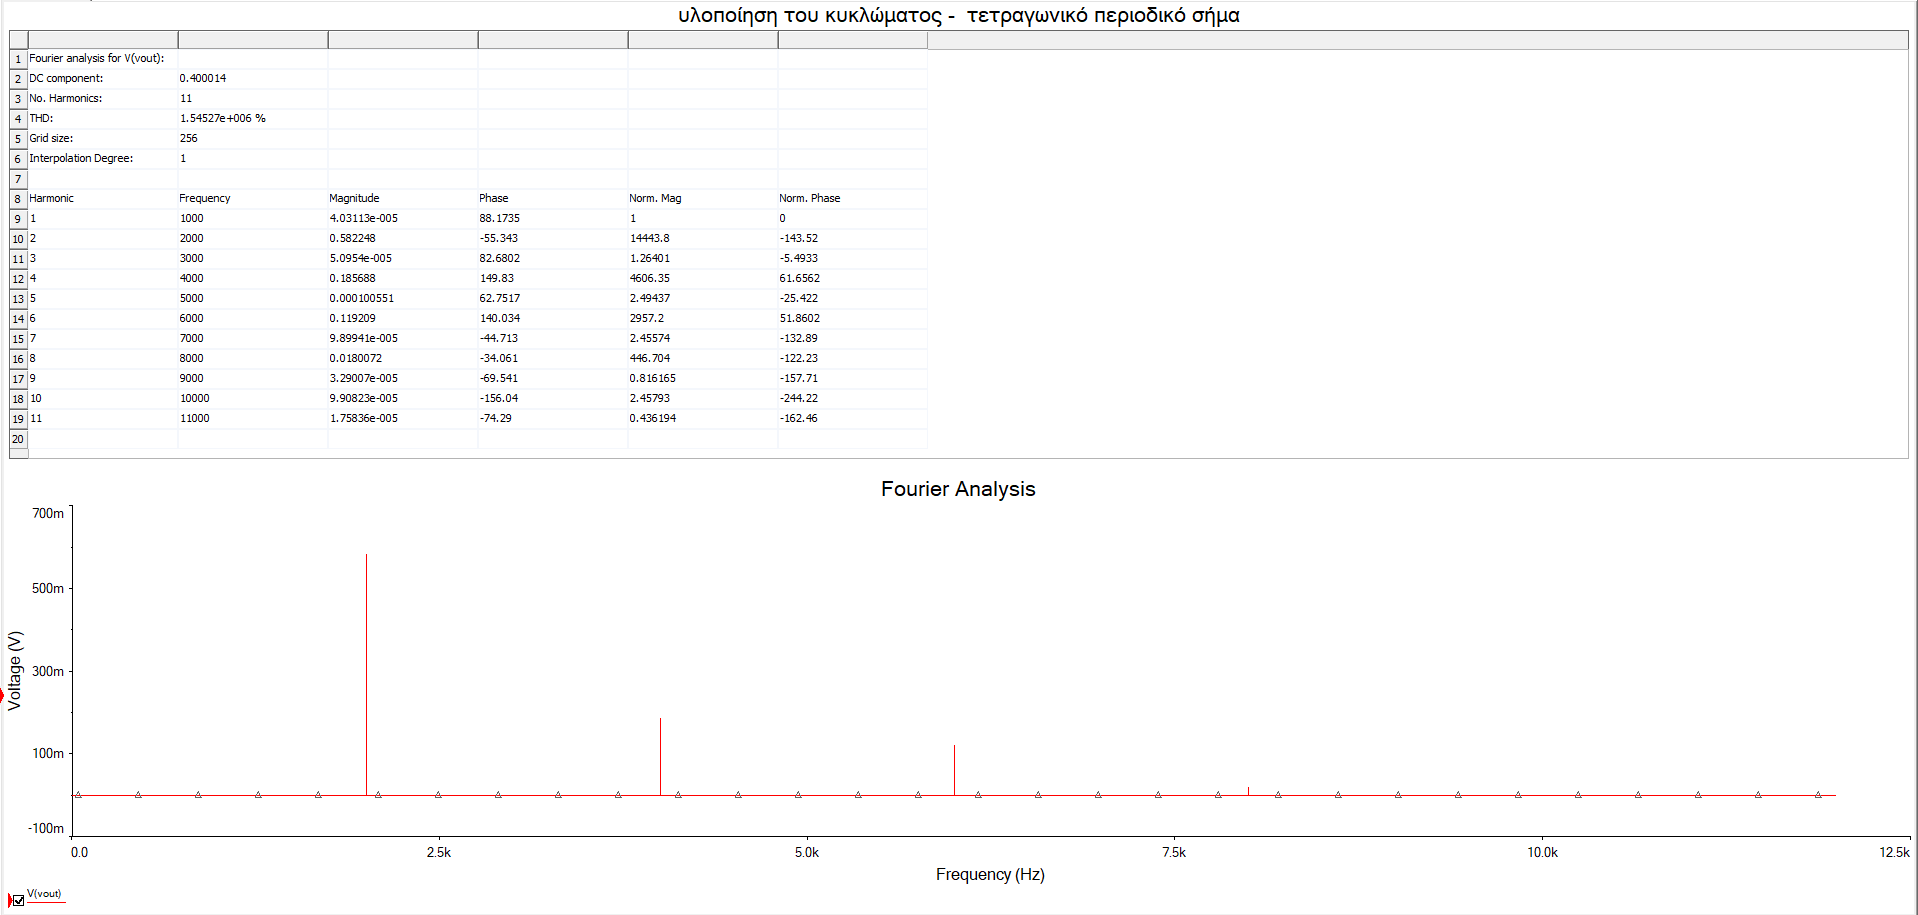
\includegraphics[width=160mm,scale=2]{multisim8.png}
\end{figure*} 
\clearpage


































































































































































































































%%%%%%%
%%%%%%%
%%%%%%%
%%%%%%%
%%%%%%%
%%%%%%%
%%%%%%%
%%%%%%%
%%%%%%%
%%%%%%%
%%%%%%%
%%%%%%%
%%%%%%%
%%%%%%%
%%%%%%%
%%%%%%%
%%%%%%%
%%%%%%%
%%%%%%%
%%%%%%%
%%%%%%%
%%%%%%%
%%%%%%%
%%%%%%%
%%%%%%%
%%%%%%%
%%%%%%%
%%%%%%%
%%%%%%%
%%%%%%%
%%%%%%%
%%%%%%%
%%%%%%%
%%%%%%%
%%%%%%%
%%%%%%%
%%%%%%%
%%%%%%%
%%%%%%%
%%%%%%%
%%%%%%%
%%%%%%%
%%%%%%%
%%%%%%%
%%%%%%%
%%%%%%%
%%%%%%%
%%%%%%%
%%%%%%%
%%%%%%%
%%%%%%%
%%%%%%%
%%%%%%%
%%%%%%%
%%%%%%%
%%%%%%%
%%%%%%%
%%%%%%%
%%%%%%%
%%%%%%%
%%%%%%%
%%%%%%%
%%%%%%%
%%%%%%%
%%%%%%%
%%%%%%%
%%%%%%%
%%%%%%%
%%%%%%%
%%%%%%%
%%%%%%%
%%%%%%%
%%%%%%%
%%%%%%%
%%%%%%%
%%%%%%%
%%%%%%%
%%%%%%%
%%%%%%%
%%%%%%%
%%%%%%%
%%%%%%%
%%%%%%%
%%%%%%%
%%%%%%%
%%%%%%%
%%%%%%%
%%%%%%%
%%%%%%%
%%%%%%%
%%%%%%%
%%%%%%%
%%%%%%%
%%%%%%%
%%%%%%%
%%%%%%%
%%%%%%%
%%%%%%%
%%%%%%%
%%%%%%%
%%%%%%%
%%%%%%%
%%%%%%%
%%%%%%%
%%%%%%%
%%%%%%%
%%%%%%%
%%%%%%%
%%%%%%%
%%%%%%%
%%%%%%%
%%%%%%%
%%%%%%%
%%%%%%%
%%%%%%%
%%%%%%%
%%%%%%%
%%%%%%%
%%%%%%%
%%%%%%%
%%%%%%%
%%%%%%%
%%%%%%%
%%%%%%%
%%%%%%%
%%%%%%%
%%%%%%%
%%%%%%%
%%%%%%%
%%%%%%%
%%%%%%%
%%%%%%%
%%%%%%%
%%%%%%%
%%%%%%%
%%%%%%%
%%%%%%%
%%%%%%%
%%%%%%%
%%%%%%%
%%%%%%%
%%%%%%%
%%%%%%%
%%%%%%%
%%%%%%%
%%%%%%%
%%%%%%%
%%%%%%%
%%%%%%%
%%%%%%%
%%%%%%%
%%%%%%%
%%%%%%%
%%%%%%%
%%%%%%%
%%%%%%%
%%%%%%%
%%%%%%%
%%%%%%%
%%%%%%%
%%%%%%%
%%%%%%%
%%%%%%%
%%%%%%%
%%%%%%%
%%%%%%%
%%%%%%%
%%%%%%%
%%%%%%%
%%%%%%%
%%%%%%%
%%%%%%%
%%%%%%%
%%%%%%%
%%%%%%%
%%%%%%%
%%%%%%%
%%%%%%%
%%%%%%%
%%%%%%%
%%%%%%%
%%%%%%%
%%%%%%%
%%%%%%%
%%%%%%%
%%%%%%%
%%%%%%%
%%%%%%%
%%%%%%%
%%%%%%%
%%%%%%%
%%%%%%%
%%%%%%%
%%%%%%%
%%%%%%%
%%%%%%%
%%%%%%%
%%%%%%%
%%%%%%%
%%%%%%%
%%%%%%%
%%%%%%%
%%%%%%%
%%%%%%%
%%%%%%%
%%%%%%%
%%%%%%%
%%%%%%%
%%%%%%%
%%%%%%%
%%%%%%%
%%%%%%%
%%%%%%%
%%%%%%%
%%%%%%%
%%%%%%%
%%%%%%%
%%%%%%%
%%%%%%%
%%%%%%%
%%%%%%%
%%%%%%%
%%%%%%%
%%%%%%%
%%%%%%%
%%%%%%%
%%%%%%%
%%%%%%%
%%%%%%%
%%%%%%%
%%%%%%%
%%%%%%%
%%%%%%%
%%%%%%%
%%%%%%%
%%%%%%%
%%%%%%%
%%%%%%%
%%%%%%%
%%%%%%%
%%%%%%%
%%%%%%%
%%%%%%%
%%%%%%%
%%%%%%%
%%%%%%%
%%%%%%%
%%%%%%%
%%%%%%%
%%%%%%%
%%%%%%%
%%%%%%%
%%%%%%%
%%%%%%%
%%%%%%%
%%%%%%%
%%%%%%%
%%%%%%%
%%%%%%%
%%%%%%%
%%%%%%%
%%%%%%%
%%%%%%%
%%%%%%%
%%%%%%%
%%%%%%%
%%%%%%%
%%%%%%%
%%%%%%%
%%%%%%%
%%%%%%%
%%%%%%%
%%%%%%%
%%%%%%%
%%%%%%%
%%%%%%%
%%%%%%%
%%%%%%%
%%%%%%%
%%%%%%%
%%%%%%%
%%%%%%%
%%%%%%%
%%%%%%%
%%%%%%%
%%%%%%%
%%%%%%%
%%%%%%%
%%%%%%%
%%%%%%%
%%%%%%%
%%%%%%%
%%%%%%%
%%%%%%%
%%%%%%%
%%%%%%%
%%%%%%%
%%%%%%%
%%%%%%%
%%%%%%%
%%%%%%%
%%%%%%%
%%%%%%%
%%%%%%%
%%%%%%%
%%%%%%%
%%%%%%%
%%%%%%%
%%%%%%%
%%%%%%%
%%%%%%%
%%%%%%%
%%%%%%%
%%%%%%%
%%%%%%%
%%%%%%%
%%%%%%%
%%%%%%%
%%%%%%%
%%%%%%%
%%%%%%%
%%%%%%%
%%%%%%%
%%%%%%%
%%%%%%%
%%%%%%%
%%%%%%%
%%%%%%%
%%%%%%%
%%%%%%%
%%%%%%%
%%%%%%%
%%%%%%%
%%%%%%%
%%%%%%%
%%%%%%%
%%%%%%%
%%%%%%%
%%%%%%%
%%%%%%%
%%%%%%%
%%%%%%%
%%%%%%%
%%%%%%%
%%%%%%%
%%%%%%%
%%%%%%%
%%%%%%%
%%%%%%%
%%%%%%%
%%%%%%%
%%%%%%%
%%%%%%%
%%%%%%%
%%%%%%%
%%%%%%%
%%%%%%%
%%%%%%%
%%%%%%%
%%%%%%%
%%%%%%%
%%%%%%%
%%%%%%%
%%%%%%%
%%%%%%%
%%%%%%%
%%%%%%%
%%%%%%%
%%%%%%%
%%%%%%%
%%%%%%%
%%%%%%%
%%%%%%%
%%%%%%%
%%%%%%%
%%%%%%%
%%%%%%%
%%%%%%%
%%%%%%%
%%%%%%%
%%%%%%%
%%%%%%%
%%%%%%%
%%%%%%%
%%%%%%%
%%%%%%%
%%%%%%%
%%%%%%%
%%%%%%%
%%%%%%%
%%%%%%%
%%%%%%%
%%%%%%%
%%%%%%%
%%%%%%%
%%%%%%%
%%%%%%%
%%%%%%%
%%%%%%%
%%%%%%%
%%%%%%%
%%%%%%%
%%%%%%%
%%%%%%%
%%%%%%%
%%%%%%%
%%%%%%%
%%%%%%%
%%%%%%%
%%%%%%%
%%%%%%%
%%%%%%%
%%%%%%%
%%%%%%%
%%%%%%%
%%%%%%%
%%%%%%%
%%%%%%%
%%%%%%%
%%%%%%%
%%%%%%%
%%%%%%%
%%%%%%%
%%%%%%%
%%%%%%%
%%%%%%%
%%%%%%%
%%%%%%%
%%%%%%%
%%%%%%%
%%%%%%%
%%%%%%%
%%%%%%%
%%%%%%%
%%%%%%%
%%%%%%%
%%%%%%%
%%%%%%%
%%%%%%%
%%%%%%%
%%%%%%%
%%%%%%%
%%%%%%%
%%%%%%%
%%%%%%%
%%%%%%%
%%%%%%%
%%%%%%%
%%%%%%%
%%%%%%%
%%%%%%%
%%%%%%%
%%%%%%%
%%%%%%%
%%%%%%%
%%%%%%%
%%%%%%%
%%%%%%%
%%%%%%%
%%%%%%%
%%%%%%%
%%%%%%%
%%%%%%%
%%%%%%%
%%%%%%%
%%%%%%%
%%%%%%%
%%%%%%%
%%%%%%%
%%%%%%%
%%%%%%%
%%%%%%%
%%%%%%%
%%%%%%%
%%%%%%%
%%%%%%%
%%%%%%%
%%%%%%%
%%%%%%%
%%%%%%%
%%%%%%%
%%%%%%%
%%%%%%%
%%%%%%%
%%%%%%%
%%%%%%%
%%%%%%%
%%%%%%%
%%%%%%%
%%%%%%%
%%%%%%%
%%%%%%%
%%%%%%%
%%%%%%%
%%%%%%%
%%%%%%%
%%%%%%%
%%%%%%%
%%%%%%%
%%%%%%%
%%%%%%%
%%%%%%%
%%%%%%%
%%%%%%%
%%%%%%%
%%%%%%%
%%%%%%%
%%%%%%%
%%%%%%%
%%%%%%%
%%%%%%%
%%%%%%%
%%%%%%%
%%%%%%%
%%%%%%%
%%%%%%%
%%%%%%%
%%%%%%%
%%%%%%%
%%%%%%%
%%%%%%%
%%%%%%%
%%%%%%%
%%%%%%%
%%%%%%%
%%%%%%%
%%%%%%%
%%%%%%%
%%%%%%%
%%%%%%%
%%%%%%%
%%%%%%%
%%%%%%%
%%%%%%%
%%%%%%%
%%%%%%%
%%%%%%%
%%%%%%%
%%%%%%%
%%%%%%%
%%%%%%%
%%%%%%%
%%%%%%%
%%%%%%%
%%%%%%%
%%%%%%%
%%%%%%%
%%%%%%%
%%%%%%%
%%%%%%%
%%%%%%%
%%%%%%%
%%%%%%%
%%%%%%%
%%%%%%%
%%%%%%%
%%%%%%%
%%%%%%%
%%%%%%%
%%%%%%%
%%%%%%%
%%%%%%%
%%%%%%%
%%%%%%%
%%%%%%%
%%%%%%%
%%%%%%%
%%%%%%%
%%%%%%%
%%%%%%%
%%%%%%%
%%%%%%%
%%%%%%%
%%%%%%%
%%%%%%%
%%%%%%%
%%%%%%%
%%%%%%%
%%%%%%%
%%%%%%%
%%%%%%%
%%%%%%%
%%%%%%%
%%%%%%%
%%%%%%%
%%%%%%%
%%%%%%%
%%%%%%%
%%%%%%%
%%%%%%%
%%%%%%%
%%%%%%%
%%%%%%%
%%%%%%%
%%%%%%%
%%%%%%%
%%%%%%%
%%%%%%%
%%%%%%%
%%%%%%%
%%%%%%%
%%%%%%%
%%%%%%%
%%%%%%%
%%%%%%%
%%%%%%%
%%%%%%%
%%%%%%%
%%%%%%%
%%%%%%%
%%%%%%%
%%%%%%%
%%%%%%%
%%%%%%%
%%%%%%%
%%%%%%%
%%%%%%%
%%%%%%%
%%%%%%%
%%%%%%%
%%%%%%%
%%%%%%%
%%%%%%%
%%%%%%%
%%%%%%%
%%%%%%%
%%%%%%%
%%%%%%%
%%%%%%%
%%%%%%%
%%%%%%%
%%%%%%%
%%%%%%%
%%%%%%%
%%%%%%%
%%%%%%%
%%%%%%%
%%%%%%%
%%%%%%%
%%%%%%%
%%%%%%%
%%%%%%%
%%%%%%%
%%%%%%%
%%%%%%%
%%%%%%%
%%%%%%%
%%%%%%%
%%%%%%%
%%%%%%%
%%%%%%%
%%%%%%%
%%%%%%%
%%%%%%%
%%%%%%%
%%%%%%%
%%%%%%%
%%%%%%%
%%%%%%%
%%%%%%%
%%%%%%%
%%%%%%%
%%%%%%%
%%%%%%%
%%%%%%%
%%%%%%%
%%%%%%%
%%%%%%%
%%%%%%%
%%%%%%%
%%%%%%%
%%%%%%%
%%%%%%%
%%%%%%%
%%%%%%%
%%%%%%%
%%%%%%%
%%%%%%%
%%%%%%%
%%%%%%%
%%%%%%%
%%%%%%%
%%%%%%%
%%%%%%%
%%%%%%%
%%%%%%%
%%%%%%%
%%%%%%%
%%%%%%%
%%%%%%%
%%%%%%%
%%%%%%%
%%%%%%%
%%%%%%%
%%%%%%%
%%%%%%%
%%%%%%%
%%%%%%%
%%%%%%%
%%%%%%%
%%%%%%%
%%%%%%%
%%%%%%%
%%%%%%%
%%%%%%%
%%%%%%%
%%%%%%%
%%%%%%%
%%%%%%%
%%%%%%%
%%%%%%%
%%%%%%%
%%%%%%%
%%%%%%%
%%%%%%%
%%%%%%%
%%%%%%%
%%%%%%%
%%%%%%%
%%%%%%%
%%%%%%%
%%%%%%%
%%%%%%%
%%%%%%%
%%%%%%%
%%%%%%%
%%%%%%%
%%%%%%%
%%%%%%%
%%%%%%%
%%%%%%%
%%%%%%%
%%%%%%%
%%%%%%%
%%%%%%%
%%%%%%%
%%%%%%%
%%%%%%%
%%%%%%%
%%%%%%%
%%%%%%%
%%%%%%%
%%%%%%%
%%%%%%%
%%%%%%%
%%%%%%%
%%%%%%%
%%%%%%%
%%%%%%%
%%%%%%%
%%%%%%%
%%%%%%%
%%%%%%%
%%%%%%%
%%%%%%%
%%%%%%%
%%%%%%%
%%%%%%%
%%%%%%%
%%%%%%%
%%%%%%%
%%%%%%%
%%%%%%%
%%%%%%%
%%%%%%%
%%%%%%%
%%%%%%%
%%%%%%%
%%%%%%%
%%%%%%%
%%%%%%%
%%%%%%%
%%%%%%%
%%%%%%%
%%%%%%%
%%%%%%%
%%%%%%%
%%%%%%%
%%%%%%%
%%%%%%%
%%%%%%%
%%%%%%%
%%%%%%%
%%%%%%%
%%%%%%%
%%%%%%%
%%%%%%%
%%%%%%%
%%%%%%%
%%%%%%%
%%%%%%%
%%%%%%%
%%%%%%%
%%%%%%%
%%%%%%%
%%%%%%%
%%%%%%%
%%%%%%%
%%%%%%%
%%%%%%%
%%%%%%%
%%%%%%%
%%%%%%%
%%%%%%%
%%%%%%%
%%%%%%%
%%%%%%%
%%%%%%%
%%%%%%%
%%%%%%%
%%%%%%%
%%%%%%%
%%%%%%%
%%%%%%%
%%%%%%%
%%%%%%%
%%%%%%%
%%%%%%%
%%%%%%%
%%%%%%%
%%%%%%%
%%%%%%%
%%%%%%%
%%%%%%%
%%%%%%%
%%%%%%%
%%%%%%%
%%%%%%%
%%%%%%%
%%%%%%%
%%%%%%%
%%%%%%%
%%%%%%%
%%%%%%%
%%%%%%%
%%%%%%%
%%%%%%%
%%%%%%%
%%%%%%%
%%%%%%%
%%%%%%%
%%%%%%%
%%%%%%%
%%%%%%%
%%%%%%%
%%%%%%%
%%%%%%%
%%%%%%%
%%%%%%%
%%%%%%%
%%%%%%%
%%%%%%%
%%%%%%%
%%%%%%%
%%%%%%%
%%%%%%%
%%%%%%%
%%%%%%%
%%%%%%%
%%%%%%%
%%%%%%%
%%%%%%%
%%%%%%%
%%%%%%%
%%%%%%%
%%%%%%%
%%%%%%%
%%%%%%%
%%%%%%%
%%%%%%%
%%%%%%%
%%%%%%%
%%%%%%%
%%%%%%%
%%%%%%%
%%%%%%%
%%%%%%%
%%%%%%%
%%%%%%%
%%%%%%%
%%%%%%%
%%%%%%%
%%%%%%%
%%%%%%%
%%%%%%%
%%%%%%%
%%%%%%%
%%%%%%%
%%%%%%%
%%%%%%%
%%%%%%%
%%%%%%%
%%%%%%%
%%%%%%%
%%%%%%%
%%%%%%%
%%%%%%%
%%%%%%%
%%%%%%%
%%%%%%%
%%%%%%%
%%%%%%%
%%%%%%%
%%%%%%%
%%%%%%%
%%%%%%%
%%%%%%%
%%%%%%%
%%%%%%%
%%%%%%%
%%%%%%%
%%%%%%%
%%%%%%%
%%%%%%%
%%%%%%%
%%%%%%%
%%%%%%%
%%%%%%%
%%%%%%%
%%%%%%%
%%%%%%%
%%%%%%%
%%%%%%%
%%%%%%%
%%%%%%%
%%%%%%%
%%%%%%%
%%%%%%%
%%%%%%%
%%%%%%%
%%%%%%%
%%%%%%%
%%%%%%%
%%%%%%%
%%%%%%%
%%%%%%%
%%%%%%%
%%%%%%%
%%%%%%%
%%%%%%%
%%%%%%%
%%%%%%%
%%%%%%%
%%%%%%%
%%%%%%%
%%%%%%%
%%%%%%%
%%%%%%%
%%%%%%%
%%%%%%%
%%%%%%%
%%%%%%%
%%%%%%%
%%%%%%%
%%%%%%%
%%%%%%%
%%%%%%%
%%%%%%%
%%%%%%%
%%%%%%%
%%%%%%%
%%%%%%%
%%%%%%%
%%%%%%%
%%%%%%%
%%%%%%%
%%%%%%%
%%%%%%%
%%%%%%%
%%%%%%%
%%%%%%%
%%%%%%%
%%%%%%%
%%%%%%%
%%%%%%%
%%%%%%%
%%%%%%%
%%%%%%%
%%%%%%%
%%%%%%%
%%%%%%%
%%%%%%%
%%%%%%%
%%%%%%%
%%%%%%%
%%%%%%%
%%%%%%%
%%%%%%%
%%%%%%%
%%%%%%%
%%%%%%%
%%%%%%%
%%%%%%%
%%%%%%%
%%%%%%%
%%%%%%%
%%%%%%%
%%%%%%%
%%%%%%%
%%%%%%%
%%%%%%%
%%%%%%%
%%%%%%%
%%%%%%%
%%%%%%%
%%%%%%%
%%%%%%%
%%%%%%%
%%%%%%%
%%%%%%%
%%%%%%%
%%%%%%%
%%%%%%%
%%%%%%%
%%%%%%%
%%%%%%%
%%%%%%%
%%%%%%%
%%%%%%%
%%%%%%%
%%%%%%%
%%%%%%%
%%%%%%%
%%%%%%%
%%%%%%%
%%%%%%%
%%%%%%%
%%%%%%%
%%%%%%%
%%%%%%%
%%%%%%%
%%%%%%%
%%%%%%%
%%%%%%%
%%%%%%%
%%%%%%%
%%%%%%%
%%%%%%%
%%%%%%%
%%%%%%%
%%%%%%%
%%%%%%%
%%%%%%%
%%%%%%%
%%%%%%%
%%%%%%%
%%%%%%%
%%%%%%%
%%%%%%%
%%%%%%%
%%%%%%%
%%%%%%%
%%%%%%%
%%%%%%%
%%%%%%%
%%%%%%%
%%%%%%%
%%%%%%%
%%%%%%%
%%%%%%%
%%%%%%%
%%%%%%%
%%%%%%%
%%%%%%%
%%%%%%%
%%%%%%%
%%%%%%%
%%%%%%%
%%%%%%%
%%%%%%%
%%%%%%%
%%%%%%%
%%%%%%%
%%%%%%%
%%%%%%%
%%%%%%%
%%%%%%%
%%%%%%%
%%%%%%%
%%%%%%%
%%%%%%%
%%%%%%%
%%%%%%%
%%%%%%%
%%%%%%%
%%%%%%%
%%%%%%%
%%%%%%%
%%%%%%%
%%%%%%%
%%%%%%%
%%%%%%%
%%%%%%%
%%%%%%%
%%%%%%%
%%%%%%%
%%%%%%%
%%%%%%%
%%%%%%%
%%%%%%%










\section*{Εργασία \#2 Σχεδίαση Ζωνοδιαβατών φίλτρων}

\addcontentsline{toc}{section}{Εργασία \#2 Σχεδίαση Ζωνοδιαβατών φίλτρων}
\begin{equation*}
\\
\end{equation*}

\begin{center}
ΖΩΝΟΔΙΑΒΑΤΟ ΦΙΛΤΡΟ CHEBYCHEV
\end{center}
\large{}
Να σχεδιασθεί ένα ζωνοδιαβατό φίλτρο Chebyshev το οποίο να πληροί τις παρακάτω προδιαγραφές συχνότητας και απόσβεσης \\[0.4\baselineskip]
$f_0$ = 900Hz    ,      $f_1$ = 825Hz  , \\[0.4\baselineskip]
$f_2$ = 981.81Hz    ,      $f_3$ = 743.88Hz , $f_4$ = 1088.88Hz \\[0.4\baselineskip]
και \\[0.4\baselineskip]
$a_{max}$ = 0.6944 dB   ,     $a_{min}$ = 29.611 dB \\[0.4\baselineskip]



\subsection*{A. Αναλυτική Σχεδίαση του Φίλτρου}
\addcontentsline{toc}{subsection}{A. Αναλυτική Σχεδίαση του Φίλτρου} 
  \subsection*{$\bullet$Υπολογισμός της Συνάρτησης Μεταφοράς}
 
 \addcontentsline{toc}{subsection}{$\bullet$Υπολογισμός της Συνάρτησης Μεταφοράς} 

\begin{equation*}
ω_1 = 2πf_1 \Rightarrow \boxed{ω_1 = 5183.6 rad/s}
\end{equation*}
\begin{equation*}
ω_2 = 2πf_2 \Rightarrow \boxed{ω_2 = 6168.9 rad/s}
\end{equation*}
\begin{equation*}
ω_3 = 2πf_3 \Rightarrow \boxed{ω_3 = 4673.9 rad/s}
\end{equation*}
\begin{equation*}
ω_4 = 2πf_4 \Rightarrow \boxed{ω_4 = 6841.6 rad/s}
\end{equation*}
Πρόκειται να υλοποιήσουμε ενα ζωνοδιαβατό φίλτρο για το οποίο:
\begin{itemize}
  \item η απόκριση του φίλτρου στην ζώνη διόδου θα έχει απόσβεση $\leq a_{max}$ δηλαδή είναι μικρότερη απο ένα ανώτερο όριο $a_{max}$ 
  \item η απόκριση του φίλτρου στην ζώνη αποκοπής θα έχει απόσβεση $\geq a_{min}$ δηλαδή είναι μεγαλύτερη απο ένα κατώτερο όριο $a_{min}$
  \item η ζώνη διόδου θα καθορίζεται από τις συχνότητες $ω_1$ και $ω_2$
     
\end{itemize}
Για τις προδιαγραφές της πρωτότυπης απόκρισης έχουμε:
\begin{equation*}
\boxed{Ω_p = 1} \enspace 
\end{equation*}
\begin{equation*}
Ω_S = \frac{ω_4 - ω_3}{ω_2 - ω_1} \Rightarrow \boxed{Ω_S = 2.2}
\end{equation*}
\begin{equation*}
ω_0 = \sqrt{ω_1 \cdot ω_2} \Rightarrow \boxed{ω_0 = 5654.86 rad/s}
\end{equation*}
\begin{equation*}
\boxed{bw = 985.3 rad/s}
\end{equation*}
Ως γνωστόν οι προδιαγραφές μας ταιριάζουν ακριβώς με τις προδιαγραφές ενός κατωδιαβατού φίλτρου Chebyshev, με την έννοια ότι η συχνότητα είναι κανονικοποιημένη στην μονάδα. \\
Στο πλαίσιο της διαδικασίας σχεδίασης θα πρέπει αρχικά να υπολογίσουμε την τάξη του φίλτρου που απαιτείται. Για να γίνει αυτό θα χρησιμοποιήσουμε τον παρακάτω τύπο :
\begin{equation*}
\boxed{n=\frac{cosh^{-1}[(10^{{α_{min}}/{10}}-1)/ (10^{{α_{max}}/{10}}-1)]^{1/2}}{cosh^{-1}(Ω_s)}
}
\end{equation*}
Μετά την αντικατάσταση των δεδομένων μας από τον τύπο προκύπτει η τιμή n=3.492.
Επειδή το n που προέκυψε δεν είναι ακέραιος διαλέγουμε τον αμέσως επόμενο. Δηλαδή , 
$\boxed{n = 4}$ \\
Απο τον τύπο:
\begin{equation*}
\boxed{ε = \sqrt{10^{a_{max}/10} -1}}
\end{equation*}
αντικαθιστώντας το $a_{max}$ παίρνουμε $\boxed{ε = 0.416}$
\\
Θα υπολογίσουμε τώρα την συχνότητα ημίσειας ισχύος από τον τύπο:
\begin{equation*}
\boxed{
Ω_{hp} = cosh\{\frac{1}{n}cosh^{-1}(\frac{1}{ε})\} }
\end{equation*} 
αντικαθιστώντας τα n και\textit{ ε }βρίσκουμε $\boxed{Ω_{hp}=1.0733 }$. \\
ομοια για το α
\begin{equation*}
\boxed{α = \frac{1}{n}sinh^{-1}(\frac{1}{ε})}
\end{equation*}
αντικαθιστώντας τα n και $ε$ βρίσκουμε $\boxed{ α = 0.4025}$ \\ Οι γωνίες Butterworth για n=4 είναι $ψ_k = \pm 22.5^o$, $\pm 67.5^o$ \\ 
Οι πόλοι Chebyshev θα προκύψουν:
\begin{equation*}
s_k = -sinha \cdot cosψ_k \pm j \cdot cosha \cdot sinψ_k
\end{equation*}
\begin{equation*}
sinha = 0.4134 \enspace cosha = 1.0821
\end{equation*}
Επομένως έχουμε:
\begin{equation*}
σ_{1,2} = -0.3819 \enspace ω_{1,2} = 0.4141 \Rightarrow \boxed{s_{1,2} = -0.3819 \pm j\cdot0.4141} 
\end{equation*}
\begin{equation*}
σ_{3,4} = -0.1582 \enspace ω_{3,4} = 0.9997 \Rightarrow \boxed{s_{3,4} = -0.1582 \pm j\cdot0.9997} 
\end{equation*}
\newpage
Στην συνέχεια χρησιμοποιούμε \textbf{\textit{τον αλγόριθμο Geffe}} για $q_c$ = $\frac{{ω_0}}{bw} \Rightarrow$ δηλαδή $q_c = 5.739$ \\ 
\textbf{ΜΕΤΑΣΧΗΜΑΤΙΣΜΟΣ: } $s_{1,2} = -0.3819 \pm j\cdot 0.4141$\\
\begin{equation*}
{Σ}_{1,2} =0.3819
\end{equation*}
\begin{equation*}
{Ω}_{1,2} = 0.4141
\end{equation*}
\begin{equation*}
{C}_{1,2} = {Σ^2}_{1,2} + {Ω^2}_{1,2} \Rightarrow \boxed{{C}_{1,2} = 0.3173}
\end{equation*}
\begin{equation*}
{D}_{1,2} = \frac{2 \cdot {Σ}_{1,2}}{q_c} \Rightarrow \boxed{{D}_{1,2} = 0.1331}
\end{equation*}
\begin{equation*}
{E}_{1,2} = 4 +\frac{{C}_{1,2}}{{q^2}_c} \Rightarrow \boxed{{E}_{1,2} = 4.0096}
\end{equation*}
\begin{equation*}
{G}_{1,2} = \sqrt{{E^2}_{1,2} - 4{D^2}_{1,2}} \Rightarrow \boxed{{G}_{1,2} = 4.0007}
\end{equation*}
\begin{equation*}
{Q}_{1,2} = \frac{1}{{D}_{1,2}} \sqrt{\frac{1}{2}({E}_{1,2}+{G}_{1,2})} \Rightarrow \boxed{{Q}_{1,2} = 15.034}
\end{equation*}
\begin{equation*}
k_{1,2} = \frac{Σ_{1,2} \cdot Q_{1,2}}{q_c} \Rightarrow \boxed{k_{1,2} = 1.0006}
\end{equation*}
\begin{equation*}
W_{1,2} = k_{1,2} + \sqrt{{k^2}_{1,2}-1} \Rightarrow 
\boxed{W_{1,2} = 1.0367}  
\end{equation*}
\begin{equation*}
ω_{01\{1,2\}} = \frac{1}{W_{1,2}}\cdot ω_0 \Rightarrow \boxed{ω_{01\{1,2\}} = 5454.4 rad/s}
\end{equation*}
\begin{equation*}
ω_{02\{1,2\}} = W_{1,2} \cdot ω_0  \Rightarrow \boxed{ω_{02\{1,2\}} = 5862.6 rad/s}  
\end{equation*}
\textbf{ΜΕΤΑΣΧΗΜΑΤΙΣΜΟΣ: } $s_{3,4} =  -0.1582 \pm j\cdot0.9997$\\
\begin{equation*}
{Σ}_{3,4} = 0.1582
\end{equation*}
\begin{equation*}
{Ω}_{3,4} = 0.9997
\end{equation*}
\begin{equation*}
{C}_{3,4} = {Σ^2}_{3,4} + {Ω^2}_{3,4} \Rightarrow \boxed{{C}_{3,4} = 1.0245}
\end{equation*}
\begin{equation*}
{D}_{3,4} = \frac{2 \cdot {Σ}_{3,4}}{q_c} \Rightarrow \boxed{{D}_{3,4} = 0.0551}
\end{equation*}
\begin{equation*}
{E}_{3,4} = 4 +\frac{{C}_{3,4}}{{q^2}_c} \Rightarrow \boxed{{E}_{3,4} = 4.0311}
\end{equation*}
\begin{equation*}
{G}_{3,4} = \sqrt{{E^2}_{3,4} - 4{D^2}_{3,4}} \Rightarrow \boxed{{G}_{3,4} = 4.0295}
\end{equation*}
\begin{equation*}
{Q}_{3,4} = \frac{1}{{D}_{3,4}} \sqrt{\frac{1}{2}({E}_{3,4}+{G}_{3,4})} \Rightarrow \boxed{{Q}_{3,4} = 36.4095}
\end{equation*}
\begin{equation*}
k_{3,4} = \frac{Σ_{3,4} \cdot Q_{3,4}}{q_c} \Rightarrow \boxed{k_{3,4} = 1.0037}
\end{equation*}
\begin{equation*}
W_{3,4} = k_{3,4} + \sqrt{{k^2}_{3,4}-1} \Rightarrow 
\boxed{W_{3,4} = 1.0908}  
\end{equation*}
\begin{equation*}
ω_{01\{3,4\}} = \frac{1}{W_{3,4}}\cdot ω_0 \Rightarrow \boxed{ω_{01\{3,4\}} = 5183.7 rad/s}
\end{equation*}
\begin{equation*}
ω_{02\{3,4\}} = W_{3,4} \cdot ω_0  \Rightarrow \boxed{ω_{02\{3,4\}} = 6168.8 rad/s}  
\end{equation*}
Οι πόλοι της συνάρτησης μεταφοράς , οι γωνίες καθώς και τα αντίστοιχα Q των ριζών προκύπτουν και παρουσιάζονται στον παρακάτω πίνακα:
\begin{center}

 \begin{tabular}{|c|c|c|}
        \hline
       \qquad $ψ_k$ \qquad \qquad &\qquad \qquad Q \qquad \qquad \qquad & \qquad \qquad $p_k$ \qquad \qquad \qquad \\
        \hline
        $\pm22.5^o$ & 15.034 & $-0.3819 \pm j\cdot0.4141$ \\
        \hline
        $\pm67.5^o$ & 36.4095 & $-0.1582 \pm j\cdot0.9997$\\
        \hline
        
        \end{tabular}
\end{center}
Άρα η συνάρτηση μεταφοράς που πρέπει να υλοποιηθεί θα αποτελείται από 4 μονάδες οι οποίες και φαίνονται παρακάτω σε διαγραμματική μορφή.
\footnotesize{}
 
\begin{center}
 \begin{changemargin}{-2.2cm}{0.5cm} 
\raisebox{-6ex}{$\to$}%
\fbox{\parbox[t]{11em}{$\enspace$ \\ Μονάδα \#1\\ $ω_{01\{1,2\}} = 5454.4 rad/s$ \\${Q}_{1,2} = 15.034$ \\$\enspace$}}%
\raisebox{-6ex}{$\to$}%
\fbox{\parbox[t]{11em}{$\enspace$ \\ Μονάδα \#2\\ $ω_{02\{1,2\}} = 5862.6 rad/s$ \\${Q}_{1,2} = 15.034$ \\$\enspace$}}%
\raisebox{-6ex}{$\to$}%
\fbox{\parbox[t]{12em}{$\enspace$ \\ Μονάδα \#3\\ $ω_{01\{3,4\}} =  5183.7 rad/s$ \\$Q_{3,4} =  36.4095$ \\$\enspace$}}%
\raisebox{-6ex}{$\to$}%
\fbox{\parbox[t]{11em}{$\enspace$ \\ Μονάδα \#4\\ $ω_{02\{3,4\}} = 6168.8 rad/s$ \\$Q_{3,4} =  36.4095$ \\$\enspace$}}%
\raisebox{-6ex}{$\to$}%
 \end{changemargin}
\end{center}
\newpage
\large{}
\subsection*{$\bullet$Υλοποίηση της Συνάρτησης Μεταφοράς}
 
 \addcontentsline{toc}{subsection}{$\bullet$Υλοποίηση της Συνάρτησης Μεταφοράς} 

\large{}
Για την υλοποίηση των μονάδων χρησιμοποιούμε το ζωνοδιαβατό κύκλωμα Delyiannis-Fried με βάση την $\boxed{στρατηγικη \enspace σχεδίασης (1)}$ αφου $a_3$ = 7 \\ 
Η κλιμακοποίηση των φίλτρων να γίνει έτσι ώστε οι μονάδες
Delyiannis-Fried
να έχουν έναν τουλάχιστον πυκνωτή με τιμή $\boxed{C = 0.01μF}$ αφού $a_2$ = 8
\\[0.4\baselineskip]
Θα θεωρήσουμε προσωρινά $ω_0 = 1$ ωστε να υλοποιήσουμε τις κανονικοποιημένες μονάδες και στην συνέχεια θα κάνουμε κλιμακοποίηση με τον συντελεστή $k_f$.
\\[0.4\baselineskip]
\large{ \underline{\textbf{Μονάδα Ι}} \\[0.4\baselineskip]}
\large{}
Βλέπουμε πως $Q_{1,2} = 15.0342$ $>$ 5 αρα θα γίνει χρήση μονάδας με ενίσχυση
\\[0.4\baselineskip]
Επιλέγουμε: $β = \frac{R_{12}}{R_{11}} \Rightarrow β = 1$ 
\begin{equation*}
C_{11} = C_{12} = 1 \enspace ,R_{11} = R_{12} = 1
\end{equation*}
\begin{equation*}
k = 1 + \frac{R_{1B}}{R_{1A}} = \frac{Q_{1,2} \cdot (β+1) - \sqrt{β}}{2 \cdot Q_{1,2} - \sqrt{β}} = \frac{Q_{1,2} \cdot (3) - \sqrt{1}}{2 \cdot Q_{1,2} - \sqrt{1}} = 1.517
\end{equation*}
\begin{equation*}
\frac{R_{1B}}{R_{1A}} = 0.517 \enspace για \enspace R_{1A} = 1 \enspace εχουμε \enspace R_{1B} = 0.517
\end{equation*}
\\[0.4\baselineskip]
\large{ {\textbf{Κλιμακοποίηση}} \\[0.4\baselineskip]}
\large{}
Για ευνόητους λόγους επιλέγουμε $k_f$ = $ω_{01\{1,2\}}$  $\Rightarrow$ $k_f$ = 5454.4\\[0.4\baselineskip] 
Για να πετύχουμε την προδιαγραφή να έχουμε τουλάχιστον εναν πυκνωτή 0.01 μF χρειάζεται
\begin{equation*}
\frac{1}{k_m \cdot k_f} C_{11}= 0.01μF
\end{equation*}
Επιλέγουμε
\begin{equation*}
k_m =18333.7 
\end{equation*}
επομένως:
\begin{equation*}
\boxed{
C_{11} = C_{12} = 0.01μF
}
\end{equation*}
\begin{equation*}
\boxed{
R_{11} = R_{12} = 18333.7   Ω
}
\end{equation*}
Για τις μονάδες $R_{1A}$ και $R_{1B}$ επιλέγουμε συντελεστή κλιμακοποίησης km = 10000 οπότε προκύπτει
\begin{equation*}
\boxed{R_{1A} = 10000   Ω} \enspace \boxed{R_{1B} = 5172.007 Ω}
\end{equation*}



\large{ \underline{\textbf{Μονάδα IΙ}} \\[0.4\baselineskip]}
\large{}
Όμοια για την μονάδα ΙΙ βλέπουμε πως $Q_{1,2} = 15.0342$ $>$ 5 αρα και γι αυτη θα γίνει χρήση μονάδας με ενίσχυση
\\[0.4\baselineskip]
Επιλέγουμε: $β = \frac{R_{22}}{R_{21}} \Rightarrow β = 1$ 
\begin{equation*}
C_{21} = C_{22} = 1 \enspace ,R_{21} = R_{22} = 1
\end{equation*}
\begin{equation*}
k = 1 + \frac{R_{2B}}{R_{2A}} = \frac{Q_{1,2} \cdot (β+1) - \sqrt{β}}{2 \cdot Q_{1,2} - \sqrt{β}} = \frac{Q_{1,2} \cdot (3) - \sqrt{1}}{2 \cdot Q_{1,2} - \sqrt{1}} = 1.517
\end{equation*}
\begin{equation*}
\frac{R_{2B}}{R_{2A}} = 0.517 \enspace για \enspace R_{2A} = 1 \enspace εχουμε \enspace R_{2B} = 0.517
\end{equation*}
\\[0.4\baselineskip]
\large{ {\textbf{Κλιμακοποίηση}} \\[0.4\baselineskip]}
\large{}
Για ευνόητους λόγους επιλέγουμε $k_f$ = $ω_{02\{1,2\}}$  $\Rightarrow$ $k_f$ = 5862.6 \\[0.4\baselineskip] 
Για να πετύχουμε την προδιαγραφή να έχουμε τουλάχιστον εναν πυκνωτή 0.01 μF χρειάζεται
\begin{equation*}
\frac{1}{k_m \cdot k_f} C_{11}= 0.01μF
\end{equation*}
Επιλέγουμε
\begin{equation*}
k_m = 17057
\end{equation*}
επομένως:
\begin{equation*}
\boxed{
C_{21} = C_{22} = 0.01μF
}
\end{equation*}
\begin{equation*}
\boxed{
R_{21} = R_{22} = 17057 Ω
}
\end{equation*}
Για τις μονάδες $R_{2A}$ και $R_{2B}$ επιλέγουμε συντελεστή κλιμακοποίησης km = 10000 οπότε προκύπτει
\begin{equation*}
\boxed{R_{2A} = 10000  Ω} \enspace \boxed{R_{2B} = 5172.007 Ω}
\end{equation*}
\\[0.4\baselineskip]
\large{ \underline{\textbf{Μονάδα IΙΙ}} \\[0.4\baselineskip]}
\large{}
Για την μονάδα ΙΙΙ ισχύει $Q_{3,4} = 36.409$ $>$ 5
συνεπώς γίνεται χρηση της μονάδας με ενίσχυση
\\[0.4\baselineskip]
Επιλέγουμε: $β = \frac{R_{32}}{R_{31}} \Rightarrow β = 1$ 
\begin{equation*}
C_{31} = C_{32} = 1 \enspace ,R_{31} = R_{32} = 1
\end{equation*}
\begin{equation*}
k = 1 + \frac{R_{3B}}{R_{3A}} = \frac{Q_{3,4} \cdot (β+1) - \sqrt{β}}{2 \cdot Q_{3,4} - \sqrt{β}} = \frac{Q_{3,4} \cdot (3) - \sqrt{1}}{2 \cdot Q_{3,4} - \sqrt{1}} = 1.506
\end{equation*}
\begin{equation*}
\frac{R_{3B}}{R_{3A}} = 0.506\enspace για \enspace R_{3A} = 1 \enspace εχουμε \enspace R_{3B} = 0.506
\end{equation*}
\\[0.4\baselineskip]
\large{ {\textbf{Κλιμακοποίηση}} \\[0.4\baselineskip]}
\large{}
Για ευνόητους λόγους επιλέγουμε $k_f$ = $ω_{01\{3,4\}}$  $\Rightarrow$ $k_f$ = 5183.7 \\[0.4\baselineskip] 
Για να πετύχουμε την προδιαγραφή να έχουμε τουλάχιστον εναν πυκνωτή 0.01 μF χρειάζεται
\begin{equation*}
\frac{1}{k_m \cdot k_f} C_{31}= 0.01μF
\end{equation*}
Επιλέγουμε
\begin{equation*}
k_m = 19291.2
\end{equation*}
επομένως:
\begin{equation*}
\boxed{
C_{31} = C_{32} = 0.01μF
}
\end{equation*}
\begin{equation*}
\boxed{
R_{31} = R_{32} = 19291.2  Ω
}
\end{equation*}
Για τις μονάδες $R_{3A}$ και $R_{3B}$ επιλέγουμε συντελεστή κλιμακοποίησης km = 10000 οπότε προκύπτει
\begin{equation*}
\boxed{R_{3A} = 10000  Ω} \enspace \boxed{R_{3B} = 5069.6194136 Ω}
\end{equation*}
\large{ \underline{\textbf{Μονάδα ΙIΙΙ}} \\[0.4\baselineskip]}
\large{}
Όμοια με την μονάδα ΙΙΙ ισχύει $Q_{3,4} =36.409$ $>$ 5
συνεπώς γίνεται χρηση της μονάδας με ενίσχυση
\\[0.4\baselineskip]
Επιλέγουμε: $β = \frac{R_{42}}{R_{41}} \Rightarrow β = 1$ 
\begin{equation*}
C_{41} = C_{42} = 1 \enspace ,R_{41} = R_{42} = 1
\end{equation*}
\begin{equation*}
k = 1 + \frac{R_{4B}}{R_{4A}} = \frac{Q_{3,4} \cdot (β+1) - \sqrt{β}}{2 \cdot Q_{3,4} - \sqrt{β}} = \frac{Q_{3,4} \cdot (3) - \sqrt{1}}{2 \cdot Q_{3,4} - \sqrt{1}} =1.506
\end{equation*}
\begin{equation*}
\frac{R_{4B}}{R_{4A}} = 0.506 \enspace για \enspace R_{4A} = 1 \enspace εχουμε \enspace R_{4B} = 0.506
\end{equation*}
\\[0.4\baselineskip]
\large{ {\textbf{Κλιμακοποίηση}} \\[0.4\baselineskip]}
\large{}
Για ευνόητους λόγους επιλέγουμε $k_f$ = $ω_{02\{3,4\}}$  $\Rightarrow$ $k_f$ = 6168.8 \\[0.4\baselineskip] 
Για να πετύχουμε την προδιαγραφή να έχουμε τουλάχιστον εναν πυκνωτή 0.01 μF χρειάζεται
\begin{equation*}
\frac{1}{k_m \cdot k_f} C_{41}= 0.01μF
\end{equation*}
Επιλέγουμε
\begin{equation*}
k_m = 16210.4 
\end{equation*}
επομένως:
\begin{equation*}
\boxed{
C_{41} = C_{42} = 0.01μF
}
\end{equation*}
\begin{equation*}
\boxed{
R_{41} = R_{42} = 16210.4   Ω
}
\end{equation*}
Για τις μονάδες $R_{4A}$ και $R_{4B}$ επιλέγουμε συντελεστή κλιμακοποίησης km = 10000 οπότε προκύπτει
\begin{equation*}
\boxed{R_{4A} = 10000   Ω} \enspace \boxed{R_{4B} = 5069.6194136 Ω}
\end{equation*}
\newpage
\subsection*{$\bullet$Ρύθμιση κέρδους}
 
 \addcontentsline{toc}{subsection}{$\bullet$Ρύθμιση κέρδους} 
 
\large{}
Μια ακόμη απαίτηση των προδιαγραφών είναι να γίνει ρύθμιση κέρδους έτσι ώστε το κέρδος του φίλτρου
στη ζώνη διέλευσης να είναι: $\boxed{\enspace 0 \enspace dB \enspace} \enspace αφου \enspace a_4 =2$.  
 \\[0.4\baselineskip]
\large{ \underline{\textbf{Συναρτήσεις Μεταφοράς Μονάδων}} \\[0.4\baselineskip]
\large{}
1. Για την πρώτη μονάδα όπως είναι γνωστό η συνάρτηση μεταφοράς είναι :
\begin{equation*}
T_1(s) = \frac{\frac{s}{R_{11}C_{11}(1-\frac{1}{k})}}{s^2 + s (\frac{1}{R_{12}C_{11}}+\frac{1}{R_{12}C_{12}}+\frac{1}{k-1} \cdot \frac{1}{R_{11}C_{11}}) + \frac{1}{R_{11}R_{12}C_{11}C_{12}}}
\end{equation*}
\begin{equation*}
\boxed{
T_1(s) = \frac{16000.4s}{s^2 +362.8s+29750754}}
\end{equation*}
2. Για την δεύτερη μονάδα όπως είναι γνωστό η συνάρτηση μεταφοράς είναι :
\begin{equation*}
T_2(s) = \frac{\frac{s}{R_{21}C_{21}(1-\frac{1}{k})}}{s^2 + s (\frac{1}{R_{22}C_{21}}+\frac{1}{R_{22}C_{22}}+\frac{1}{k-1} \cdot \frac{1}{R_{21}C_{21}}) + \frac{1}{R_{21}R_{22}C_{21}C_{22}}}
\end{equation*}
\begin{equation*}
\boxed{
T_2(s) = \frac{17198s}{s^2 +389.9s+34370949}}
\end{equation*}
3. Για την τρίτη μονάδα όπως είναι γνωστό η συνάρτηση μεταφοράς είναι :
\begin{equation*}
T_3(s) = \frac{\frac{s}{R_{31}C_{31}(1-\frac{1}{k})}}{s^2 + s (\frac{1}{R_{32}C_{31}}+\frac{1}{R_{32}C_{32}}+\frac{1}{k-1} \cdot \frac{1}{R_{31}C_{31}}) + \frac{1}{R_{31}R_{32}C_{31}C_{32}}}
\end{equation*}
\begin{equation*}
\boxed{
T_3(s) = \frac{15408.7s}{s^2 +142.3s+26870801}}
\end{equation*}
4. Για την τέταρτη μονάδα όπως είναι γνωστό η συνάρτηση μεταφοράς είναι :
\begin{equation*}
T_4(s) = \frac{\frac{s}{R_{41}C_{41}(1-\frac{1}{k})}}{s^2 + s (\frac{1}{R_{42}C_{41}}+\frac{1}{R_{42}C_{42}}+\frac{1}{k-1} \cdot \frac{1}{R_{41}C_{41}}) + \frac{1}{R_{41}R_{42}C_{41}C_{42}}}
\end{equation*}
\begin{equation*}
\boxed{
T_4(s) = \frac{18337s}{s^2 +169.4s+38054752}}
\end{equation*}
Το κέρδος προκύπτει απο τον τύπο:
\begin{equation}
|{T}_i(jω)| = \frac{\frac{k}{(k-1)R_{i}C_{i}}ω}{\sqrt{(ω_i - ω_0)^2 + (ω_0 \cdot \frac{ω_i}{Q_i})^2}}
\end{equation}
Υπολογίστηκαν τα κέρδη απο την (1):
\begin{equation*}
|T_1(jω)| = |T_2(jω)| = \frac{\frac{k}{(k-1)R_{11}C_{11}}ω_0}{\sqrt{(ω_{01\{1,2\}} - ω_0)^2 + (ω_{01\{1,2\}} \cdot \frac{ω_0}{Q_{1,2}})^2}}
\end{equation*}
\begin{equation*}
|T_3(jω)| = |T_4(jω)| = \frac{\frac{k}{(k-1)R_{31}C_{31}}ω_0}{\sqrt{(ω_{01\{3,4\}} - ω_0)^2 + (ω_{01\{3,4\}} \cdot \frac{ω_0}{Q_{3,4}})^2}}
\end{equation*}
\begin{equation*}
\boxed{
|T_1(jω)| = |T_2(jω)| =  29.883
}
\end{equation*}
\begin{equation*}
\boxed{
|T_3(jω)| = |T_4(jω)| = 16.854
}
\end{equation*}
Για να έχουμε 0 dB στην κεντρική συχνότητα θα πρέπει να αποσβέσουμε τον λόγο 
\begin{equation*}
a = \frac{1}{|T_1(jω)| \cdot  |T_2(jω)| \cdot |T_3(jω)| \cdot |T_4(jω)|  }
\end{equation*}
\\[0.1\baselineskip]
\begin{equation*}
\boxed{a = 3.77 \cdot 10^{-6}}
\end{equation*}
\textbf{Θα χρειαστεί να κάνουμε εξασθένιση της εισόδου με την παρακάτω συνδεσμολογία.}\\
\begin{figure*}[h!]
\centering
 	
  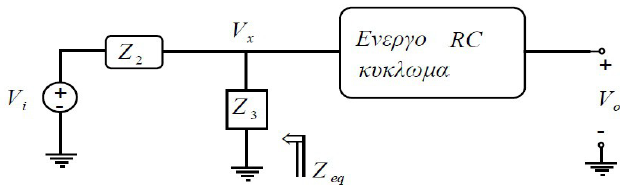
\includegraphics[width=80mm,scale=2]{kerdos.png}
\end{figure*} \\
Οπου η απόσβεση αυτή υλοποιείται για $Ζ_2 = \frac{R11}{α}$ = και $Ζ_3 = \frac{R11}{1-α}$  
\begin{equation*}
\boxed{R_{11} = Z_2 = 4863.06MΩ} \enspace \boxed{R_{13} = Z_3 = 18333.809747Ω}  
\end{equation*}
Η συνολική συνάρτηση μεταφοράς
\begin{equation*}
T_{BP}(s) = α \cdot T_1(s) \cdot T_2(s) \cdot T_3(s) \cdot T_4(s)
\end{equation*}
\small{}
\begin{changemargin}{-3.5cm}{0.5cm} 
\begin{equation*}
\boxed{
T_{BP} (s) = \frac{3.065 \cdot 10^{11} \cdot s^4}{s^8 + 1065 s^7 + 1.294\cdot10^8 \cdot s^6 + 1.03 \cdot 10^{11} \cdot s^5 + 6.234 \cdot 10^{15} \cdot s^4 + 3.293 \cdot 10^{18} \cdot s^3 + 1.324\cdot 10^{23} \cdot s^2 + 3.481 \cdot 10^{25}\cdot s + 1.046 \cdot 10^{30}
 }
 }
\end{equation*}
\end{changemargin}
\large{}
\newpage
Στο παρακάτω σχήμα φαίνεται το κανονικοποιημένο κύκλωμα στο οποίο φαίνονται οι 4 μονάδες Q enhancement χωρίς να εχει γίνει ρύθμιση του κέρδους.
\begin{figure*}[h!]
\centering
 	\advance\leftskip-4cm
  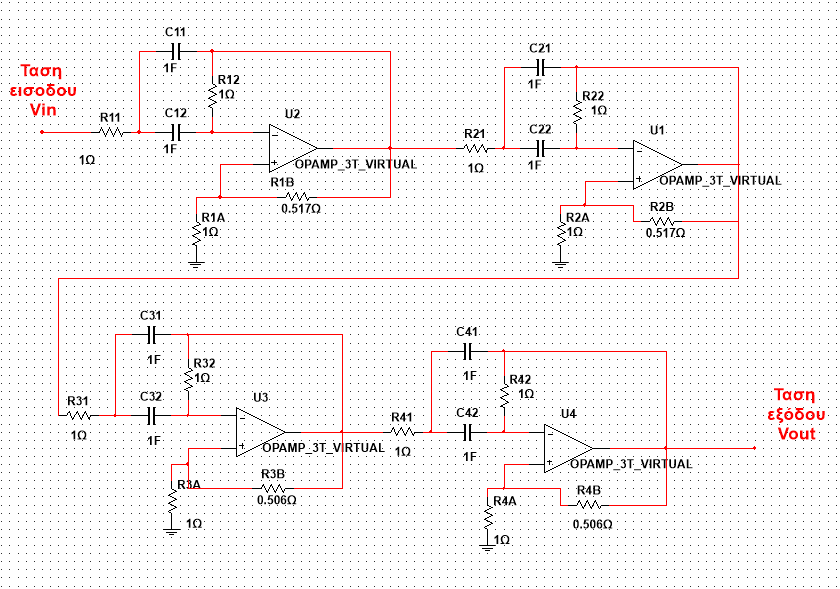
\includegraphics[width=200mm,scale=2]{kanon_bandpass2.png}
\end{figure*} 
\newpage
Στην επόμενη σελίδα εχουμε ρυθμίσει το κέρδος όπως φαίνεται στο τελικό κύκλωμα παρουσιάζουμε το επιθυμητό ζωνοδιαβατό φίλτρο Chebyshev με ότι στοιχείο είναι απαραίτητο αλλά και με τις απαιτούμενες τιμές όλων των στοιχείων για την ικανοποίηση των ζητούμενων προδιαγραφών.
\begin{figure*}[h!]
\centering
 	\advance\leftskip-4cm
  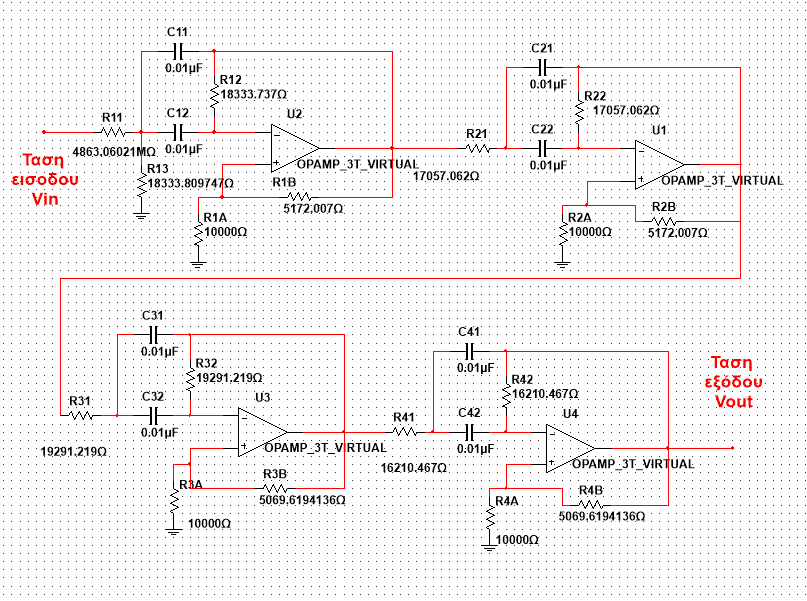
\includegraphics[width=200mm,scale=2]{nokanon_bandpass2.png}
\end{figure*} 
\newpage
\subsection*{B. Μελέτη της Συνάρτησης Μεταφοράς στο MATLAB}
\addcontentsline{toc}{subsection}{B. Μελέτη της Συνάρτησης Μεταφοράς στο MATLAB}
\large{}
Εισάγουμε στο  πρόγραμμα MATLAB τις επί μέρους συναρτήσεις μεταφοράς
\begin{equation*}
\boxed{
T_1(s) = \frac{16000.4s}{s^2 +362.8s+29750754}}
\end{equation*}
\begin{equation*}
\boxed{
T_2(s) = \frac{17198s}{s^2 +389.9s+34370949}}
\end{equation*}
 \begin{equation*}
\boxed{
T_3(s) = \frac{15408.7s}{s^2 +142.3s+26870801}}
\end{equation*}
\begin{equation*}
\boxed{
T_4(s) = \frac{18337s}{s^2 +169.4s+38054752}}
\end{equation*}
αλλά και την συνολική συνάρτησης μεταφοράς του φίλτρου 
 \small{}
\begin{changemargin}{-3.5cm}{0.5cm} 
\begin{equation*}
\boxed{
T_{BP} (s) = \frac{3.065 \cdot 10^{11} \cdot s^4}{s^8 + 1065 s^7 + 1.294\cdot10^8 \cdot s^6 + 1.03 \cdot 10^{11} \cdot s^5 + 6.234 \cdot 10^{15} \cdot s^4 + 3.293 \cdot 10^{18} \cdot s^3 + 1.324\cdot 10^{23} \cdot s^2 + 3.481 \cdot 10^{25}\cdot s + 1.046 \cdot 10^{30}
 }
 }
\end{equation*}
\end{changemargin}
\large{}
και παίρνουμε τις αποκρίσεις πλάτους σε dB. \\ Η απόκρισεις πλάτους σε dB για κάθε περίπτωση παρουσιάζονται ευθύς αμεσως. Τα παρακάτω διαγράμματα προέκυψαν στο Matlab χρησιμοποιώντας την παρεχόμενη συνάρτηση plot\_transfer\_function.m με όρισμα κάθε φορά την συνάρτηση μεταφοράς των επί μέρους συστημάτων, καθώς και τις κρίσιμες συχνότητες αυτών. 
\\[2.4\baselineskip]

\newpage

\newpage
\section*{$1^\textbf{η}$ Μονάδα - Ζωνοδιαβατό κύκλωμα Delyiannis-Fried} 
  \begin{figure*}[h!]
\centering
 	\advance\leftskip-2cm
  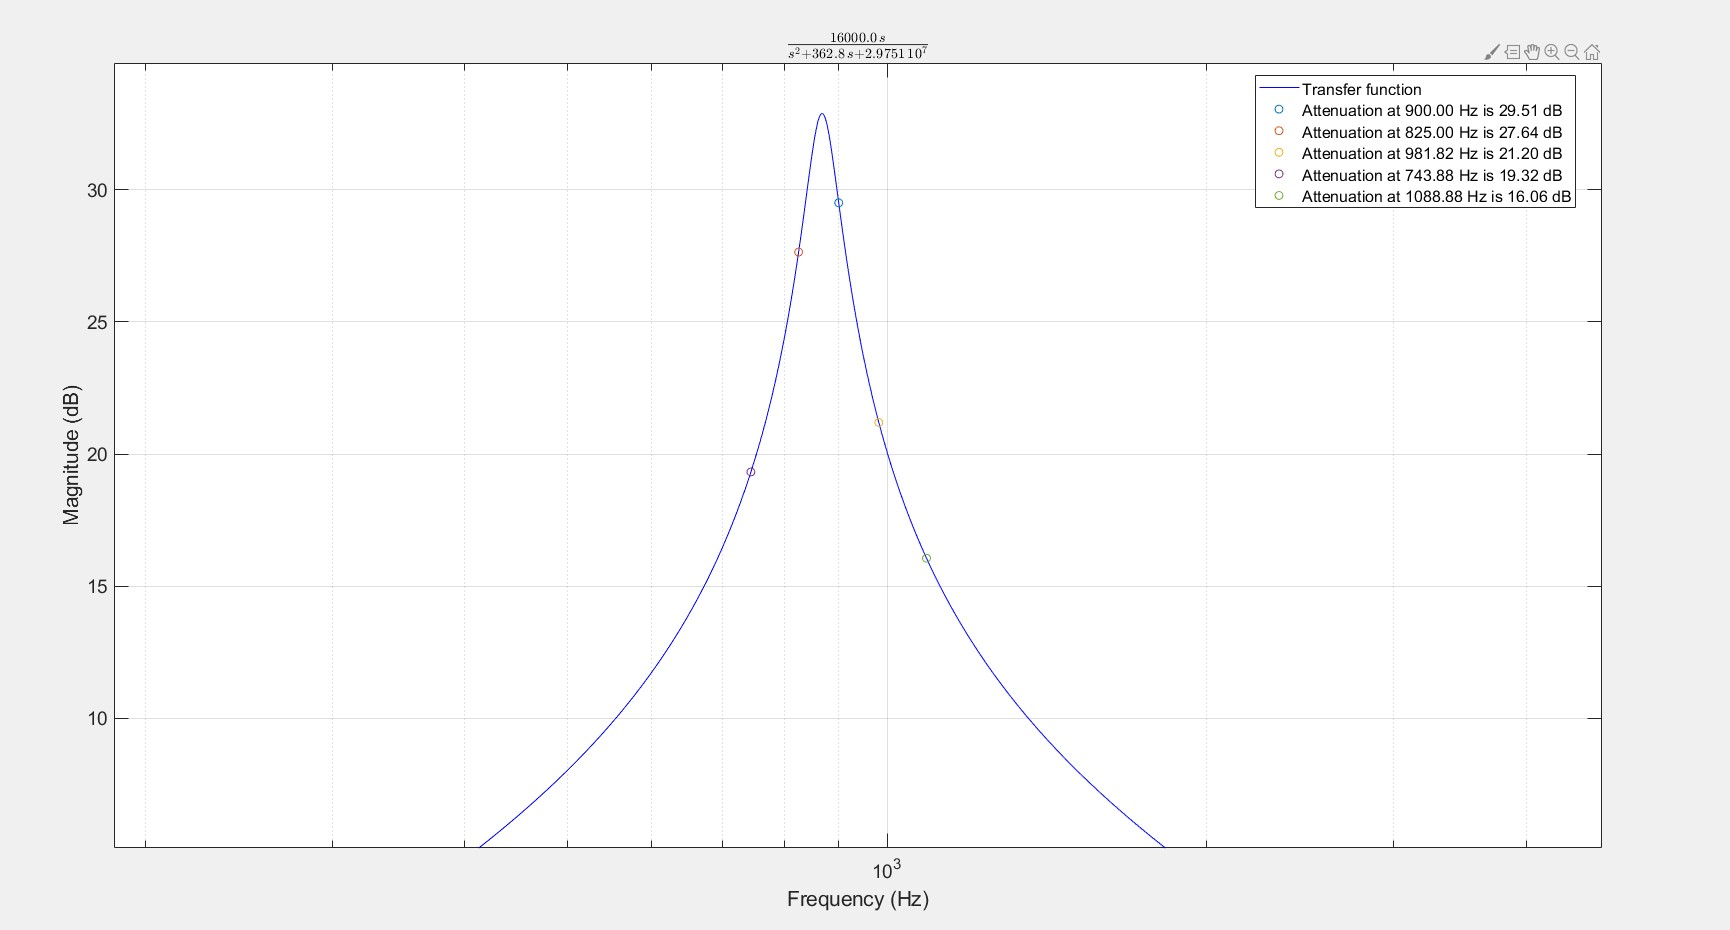
\includegraphics[width=160mm,scale=2]{thema2/matlab0.jpg}
\end{figure*} 
\normalsize{}
Στο παραπάνω διάγραμμα της $1^{ης}$ μονάδας κάνουμε ζουμ ώστε να φαίνεται ευδιάκριτα η απόκριση στις κρίσημες συχνότητες με τις κατάλληλες κλίμακες:
\large{}
  \begin{figure*}[h!]
\centering
 	\advance\leftskip-1cm
  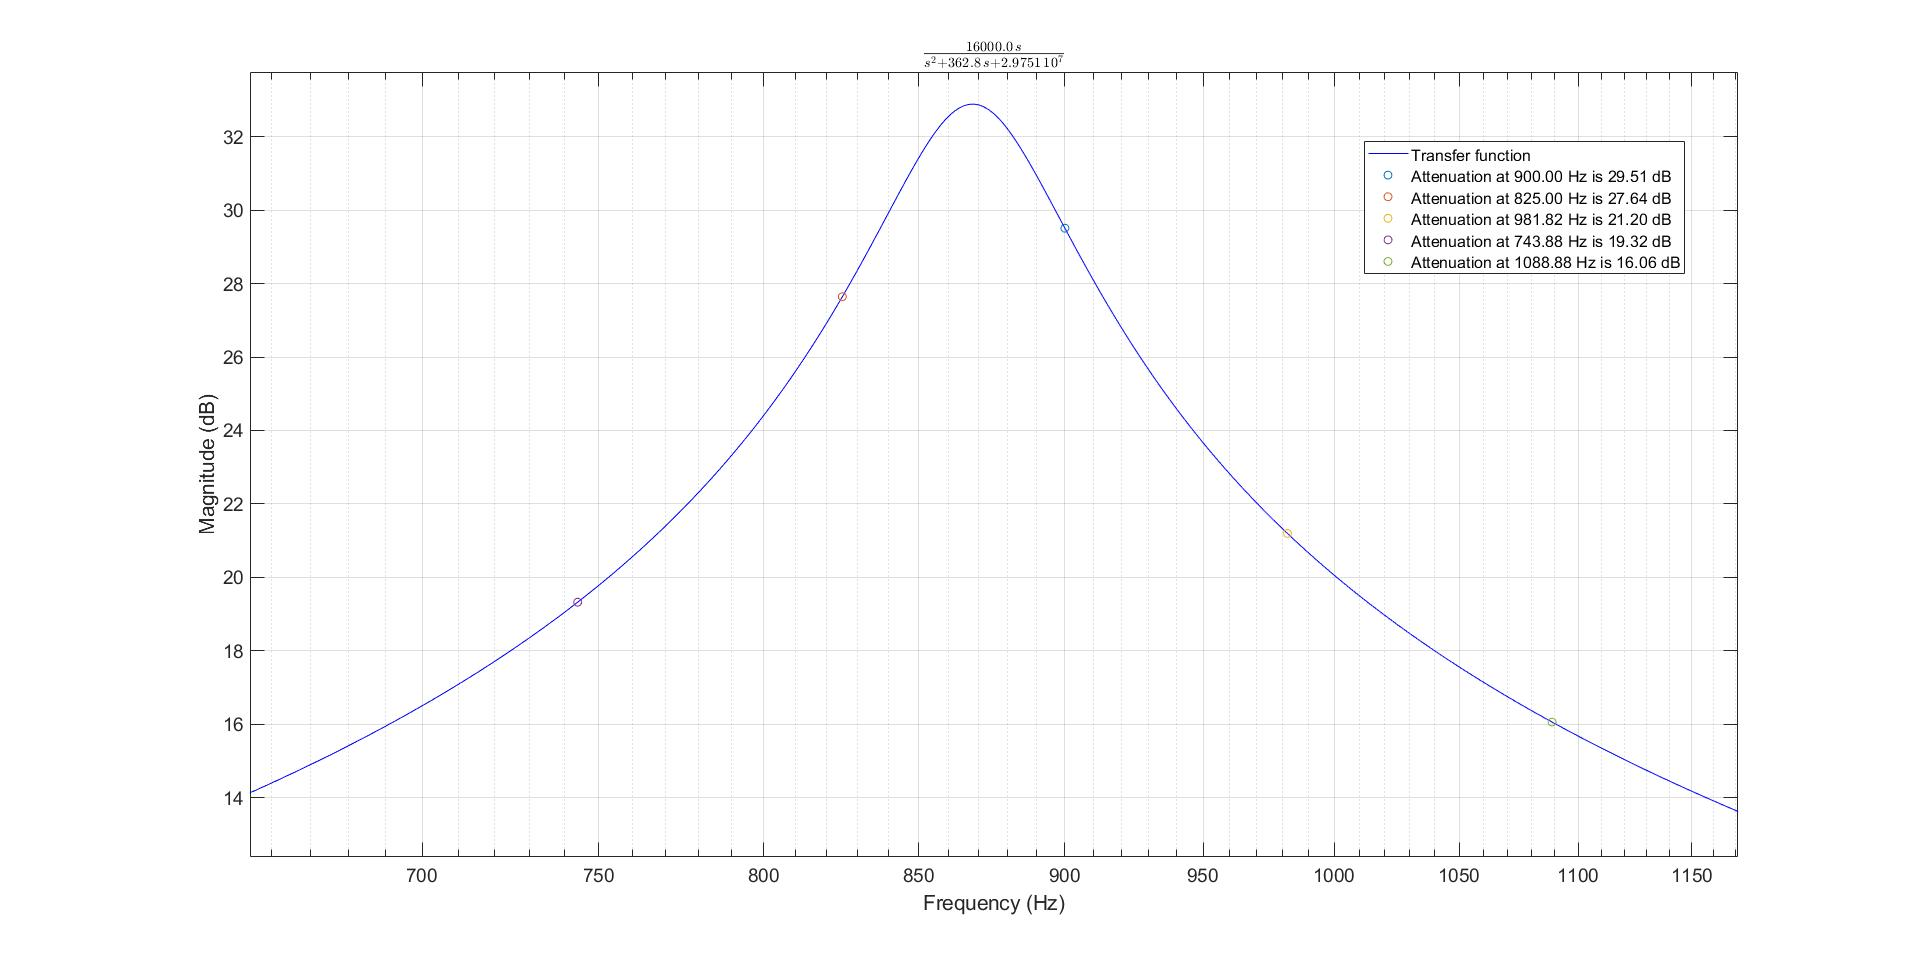
\includegraphics[width=120mm,scale=2]{thema2/z1.jpg}
\end{figure*} 
\newpage
\section*{$2^\textbf{η}$ Μονάδα - Ζωνοδιαβατό κύκλωμα Delyiannis-Fried} 
  \begin{figure*}[h!]
\centering
 	\advance\leftskip-2cm
  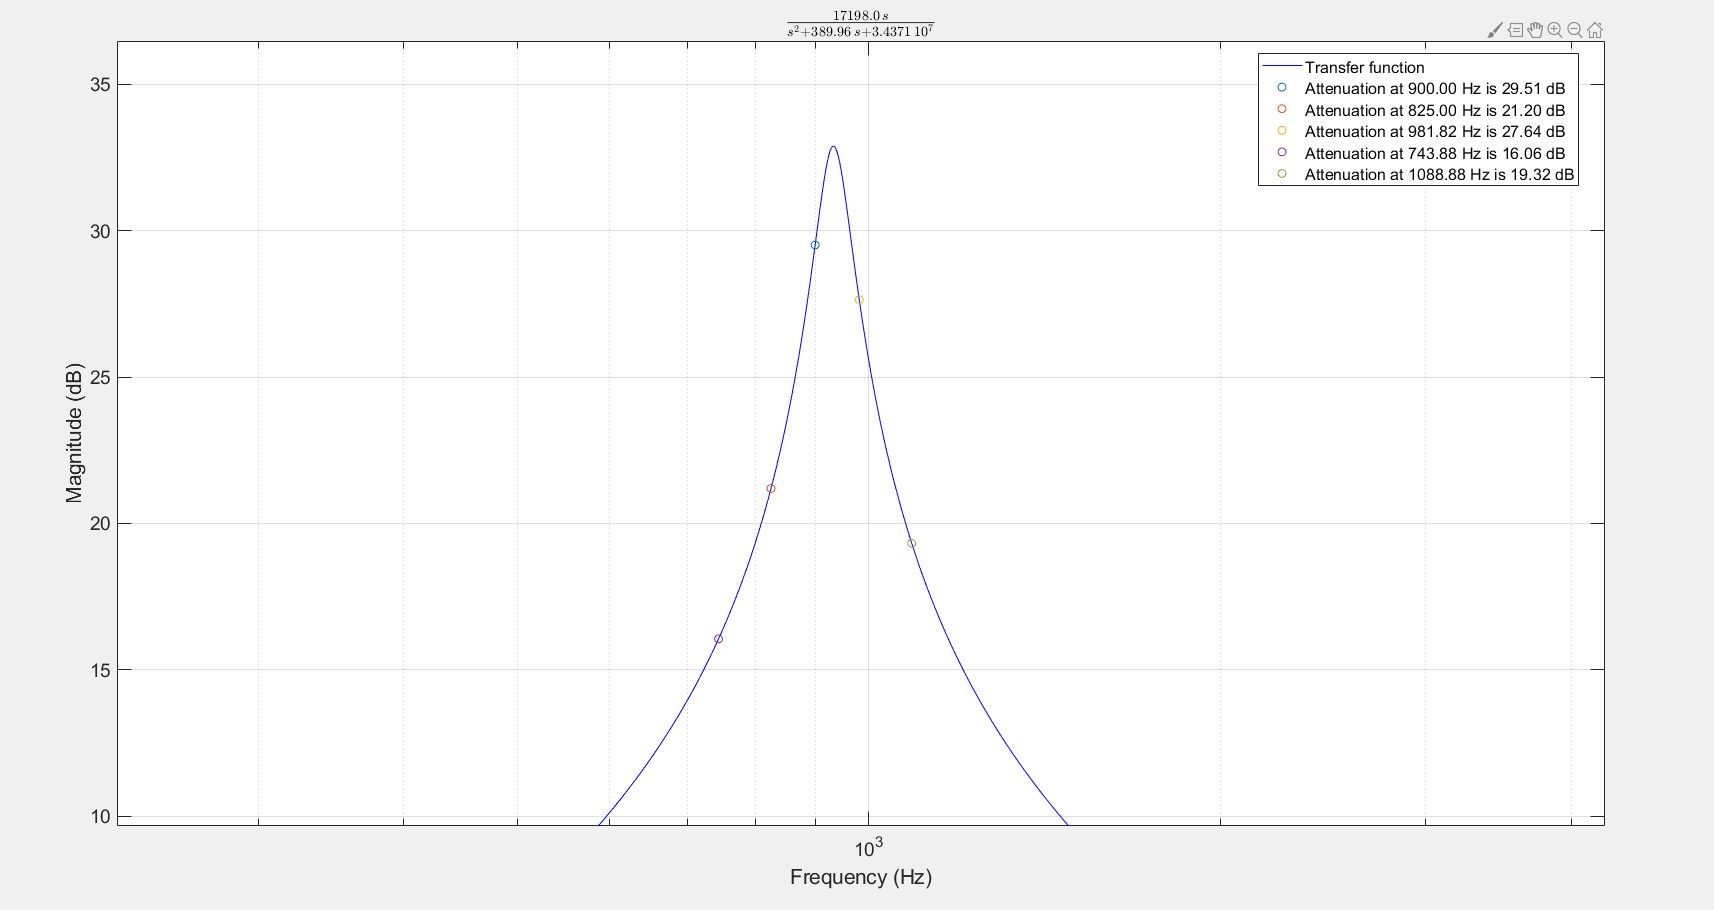
\includegraphics[width=160mm,scale=2]{thema2/matlab1.jpg}
\end{figure*} 
\normalsize{}
Στο παραπάνω διάγραμμα της $2^{ης}$ μονάδας κάνουμε ζουμ ώστε να φαίνεται ευδιάκριτα η απόκριση στις κρίσημες συχνότητες με τις κατάλληλες κλίμακες:
\large{}
  \begin{figure*}[h!]
\centering
 	\advance\leftskip-1cm
  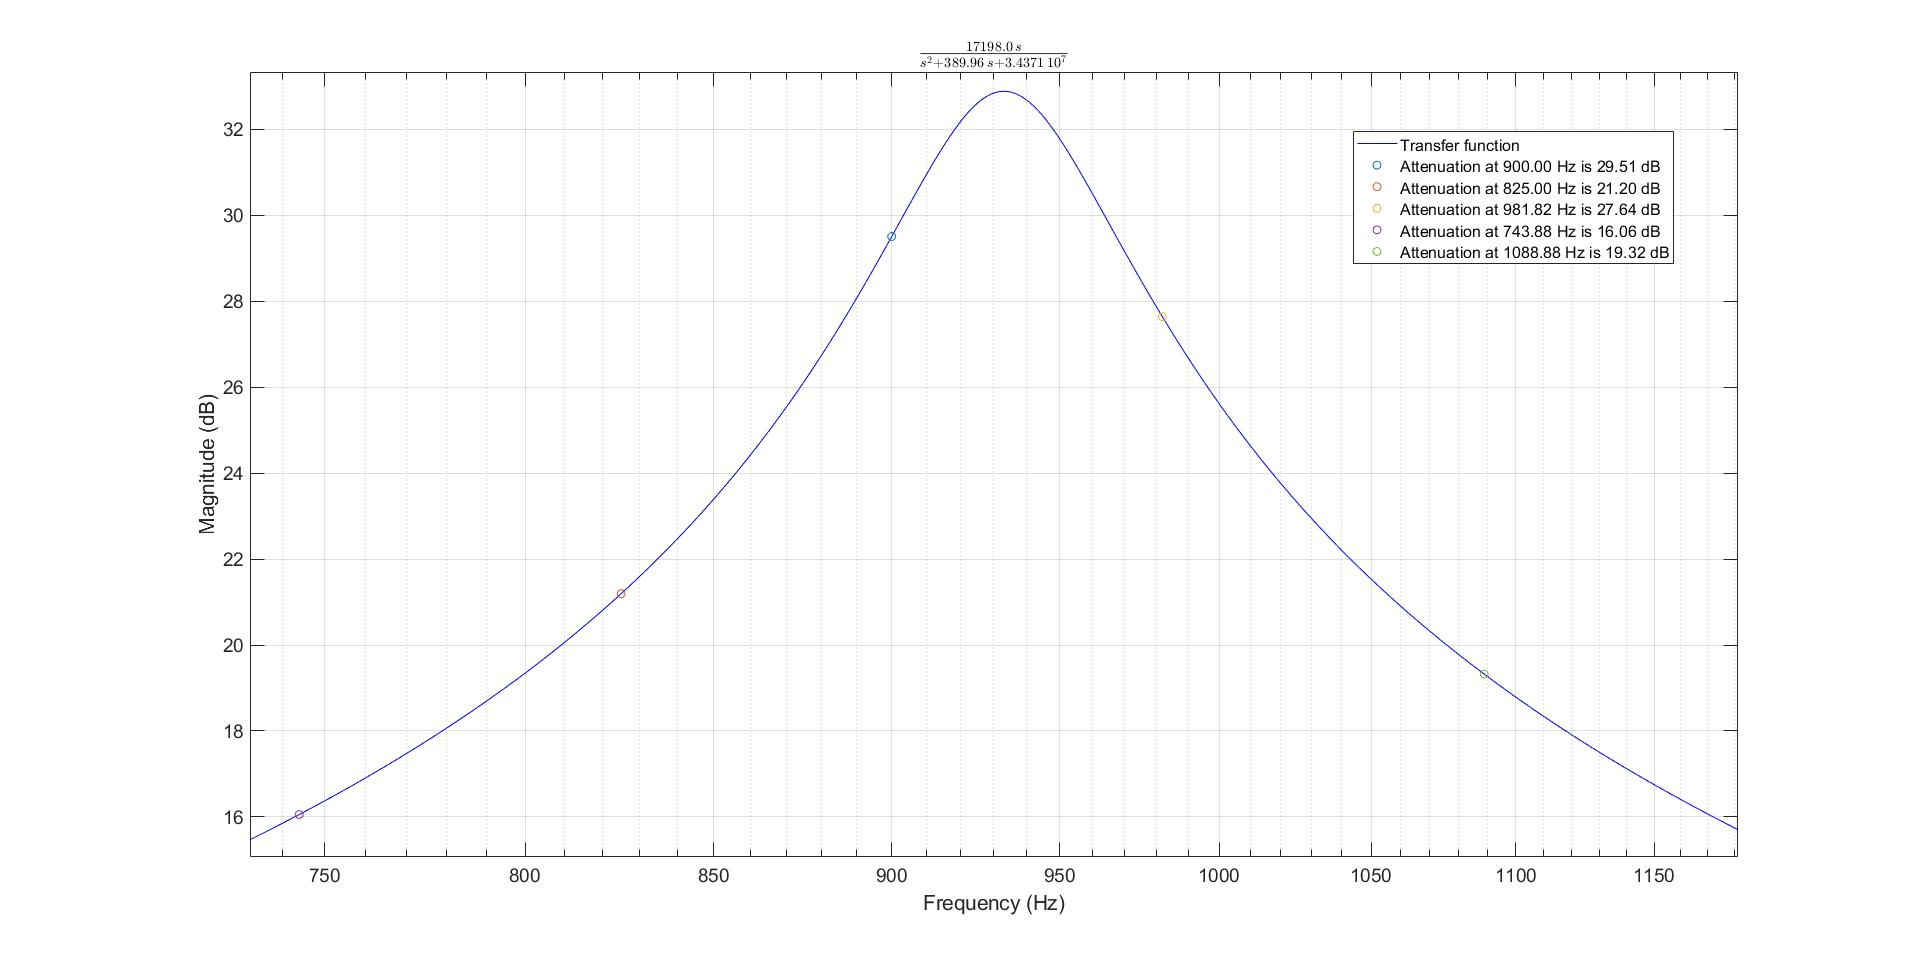
\includegraphics[width=120mm,scale=2]{thema2/z2.jpg}
\end{figure*} 
\newpage
\section*{$3^\textbf{η}$ Μονάδα - Ζωνοδιαβατό κύκλωμα Delyiannis-Fried} 
  \begin{figure*}[h!]
\centering
 	\advance\leftskip-2cm
  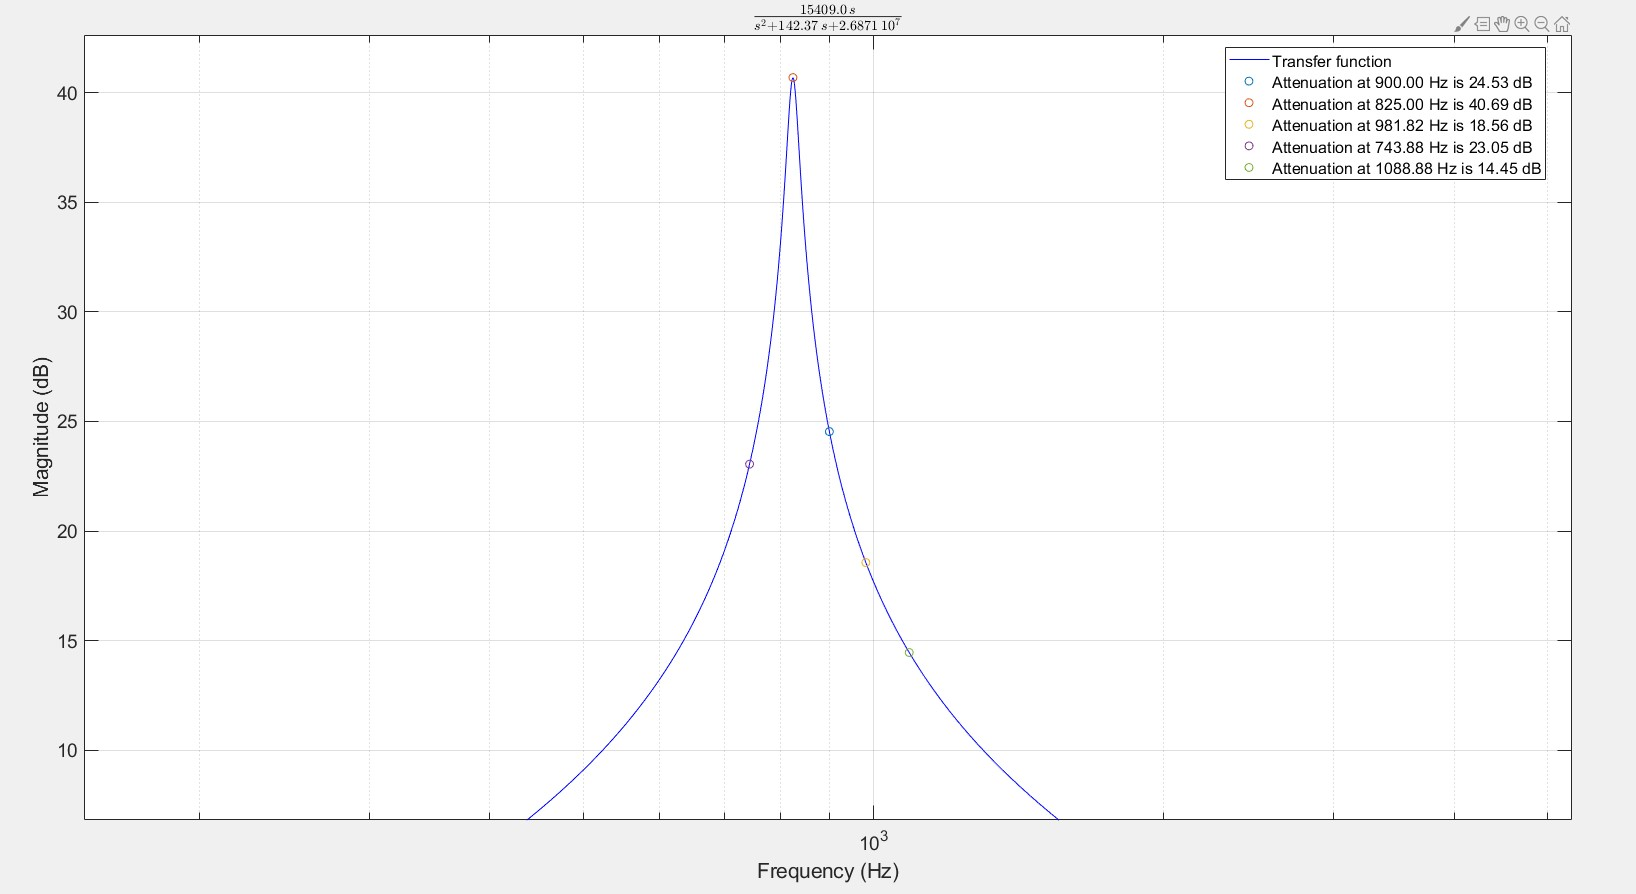
\includegraphics[width=160mm,scale=2]{thema2/matlab2.jpg}
\end{figure*}  
\normalsize{}
Στο παραπάνω διάγραμμα της $3^{ης}$ μονάδας κάνουμε ζουμ ώστε να φαίνεται ευδιάκριτα η απόκριση στις κρίσημες συχνότητες με τις κατάλληλες κλίμακες:
\large{}
  \begin{figure*}[h!]
\centering
 	\advance\leftskip-1cm
  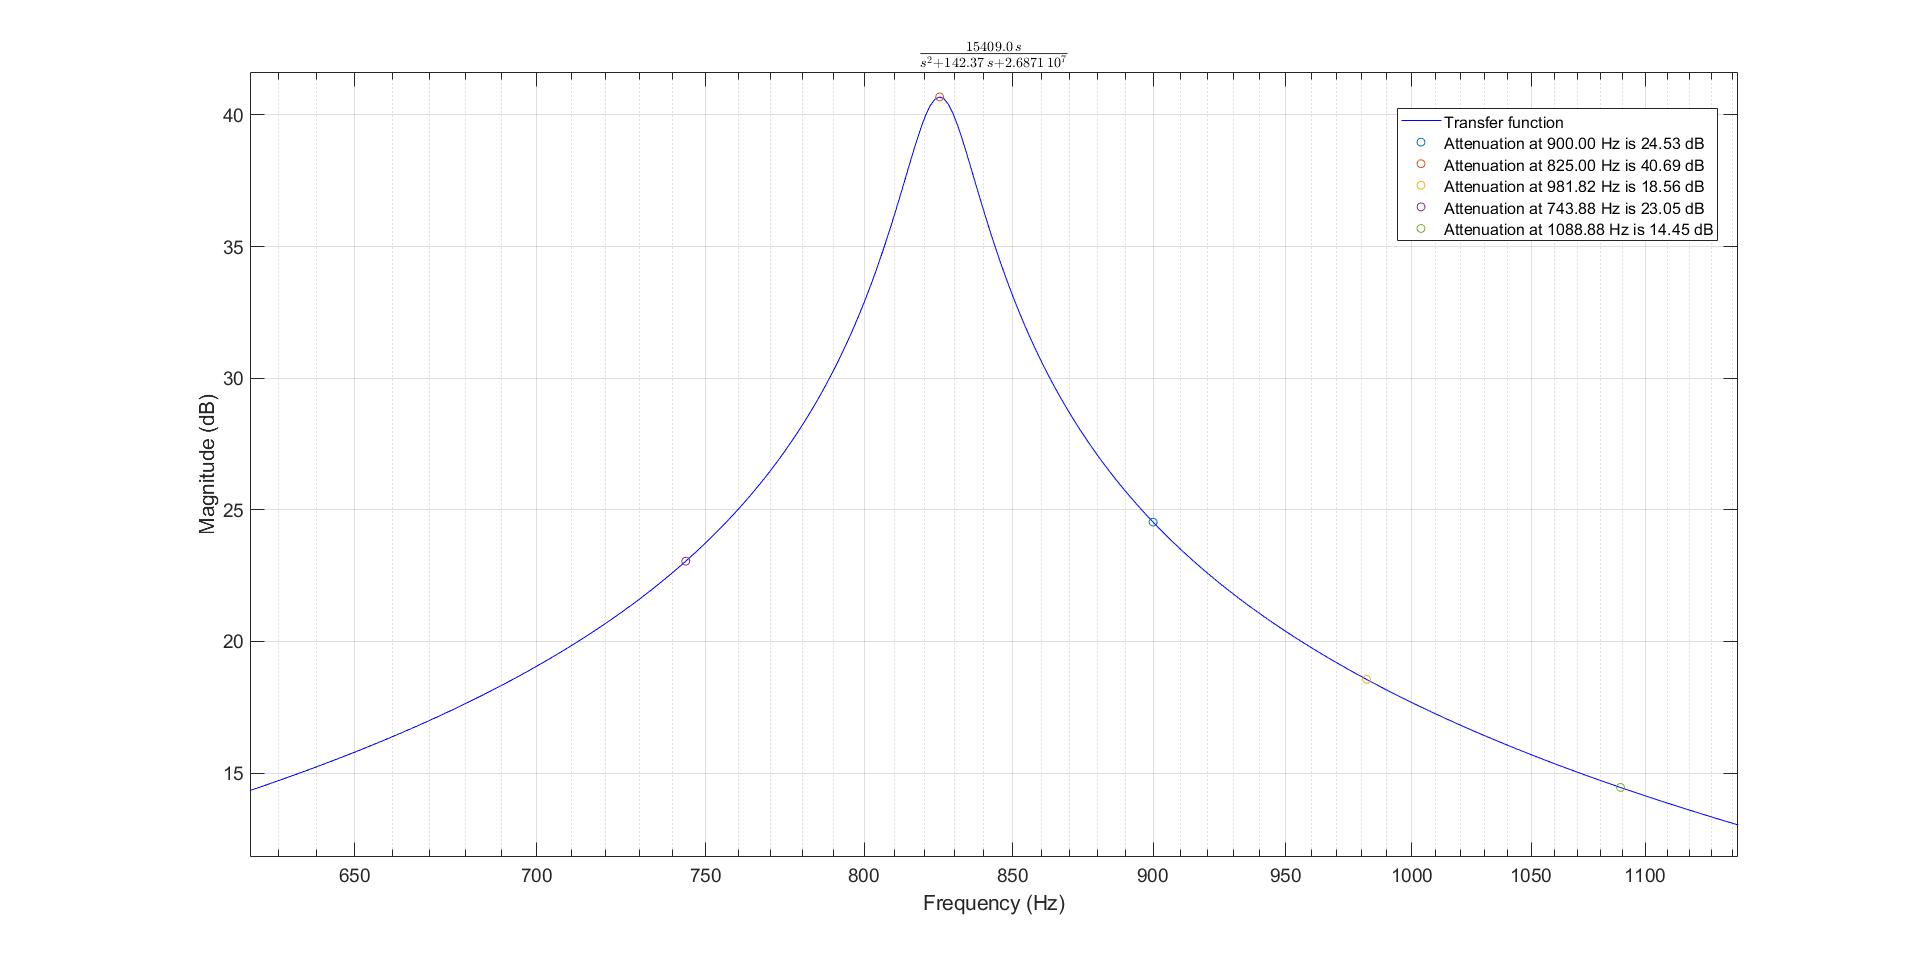
\includegraphics[width=120mm,scale=2]{thema2/z3.jpg}
\end{figure*} 
\newpage
\section*{$4^\textbf{η}$ Μονάδα - Ζωνοδιαβατό κύκλωμα Delyiannis-Fried} 
  \begin{figure*}[h!]
\centering
 	\advance\leftskip-2cm
  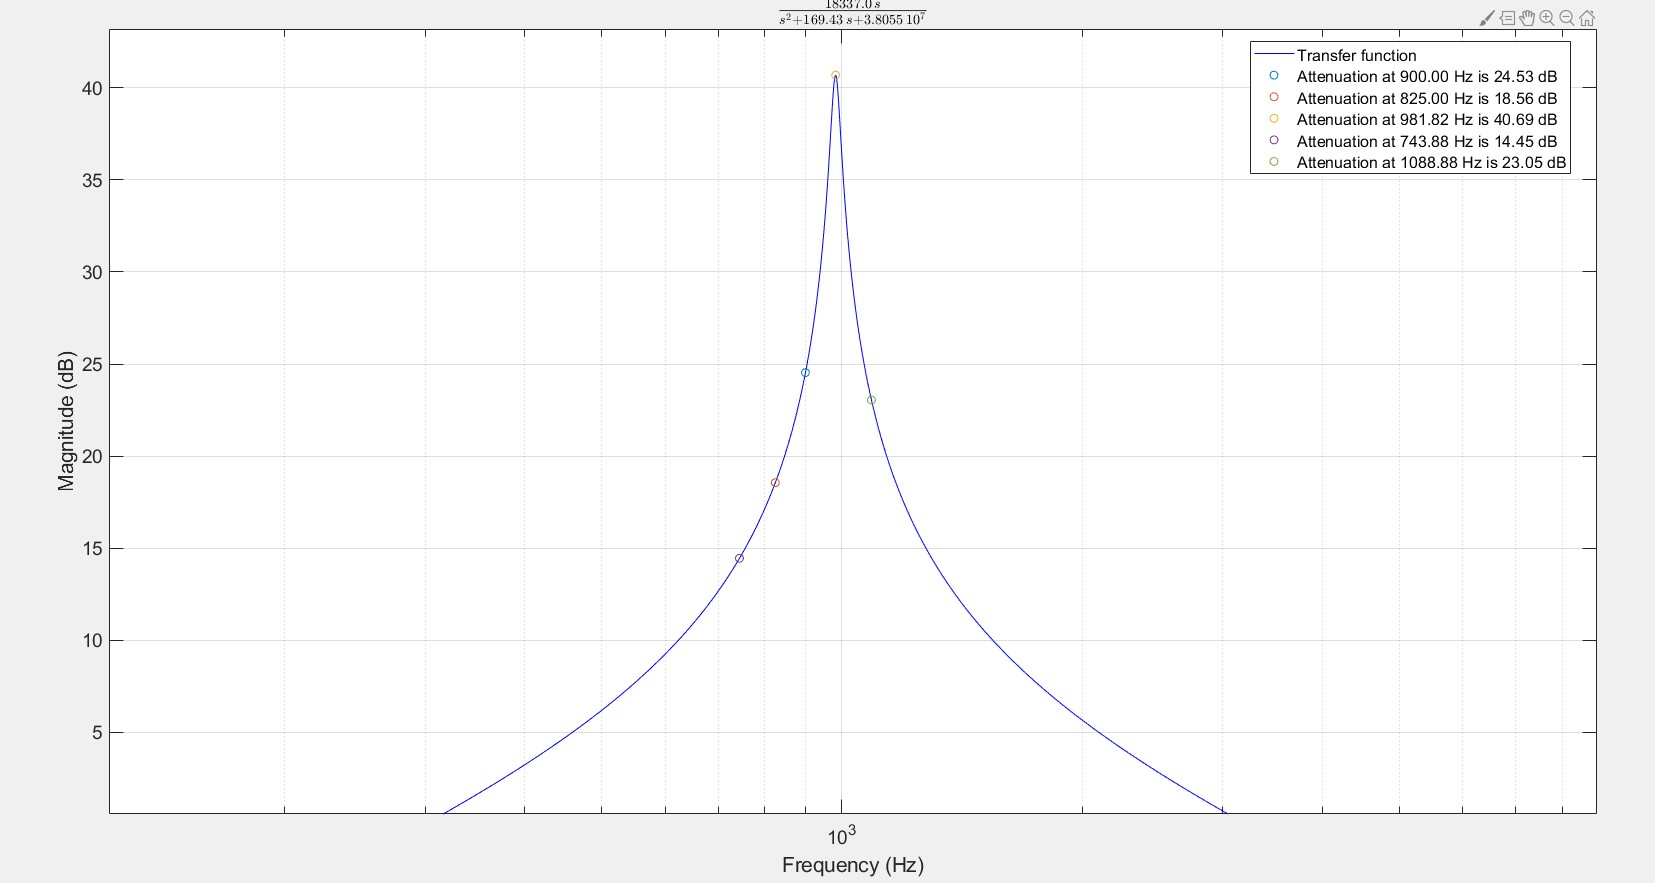
\includegraphics[width=160mm,scale=2]{thema2/matlab3.jpg}
\end{figure*} 
\normalsize{}
Στο παραπάνω διάγραμμα της $4^{ης}$ μονάδας κάνουμε ζουμ ώστε να φαίνεται ευδιάκριτα η απόκριση στις κρίσημες συχνότητες με τις κατάλληλες κλίμακες:
\large{}
  \begin{figure*}[h!]
\centering
 	\advance\leftskip-1cm
  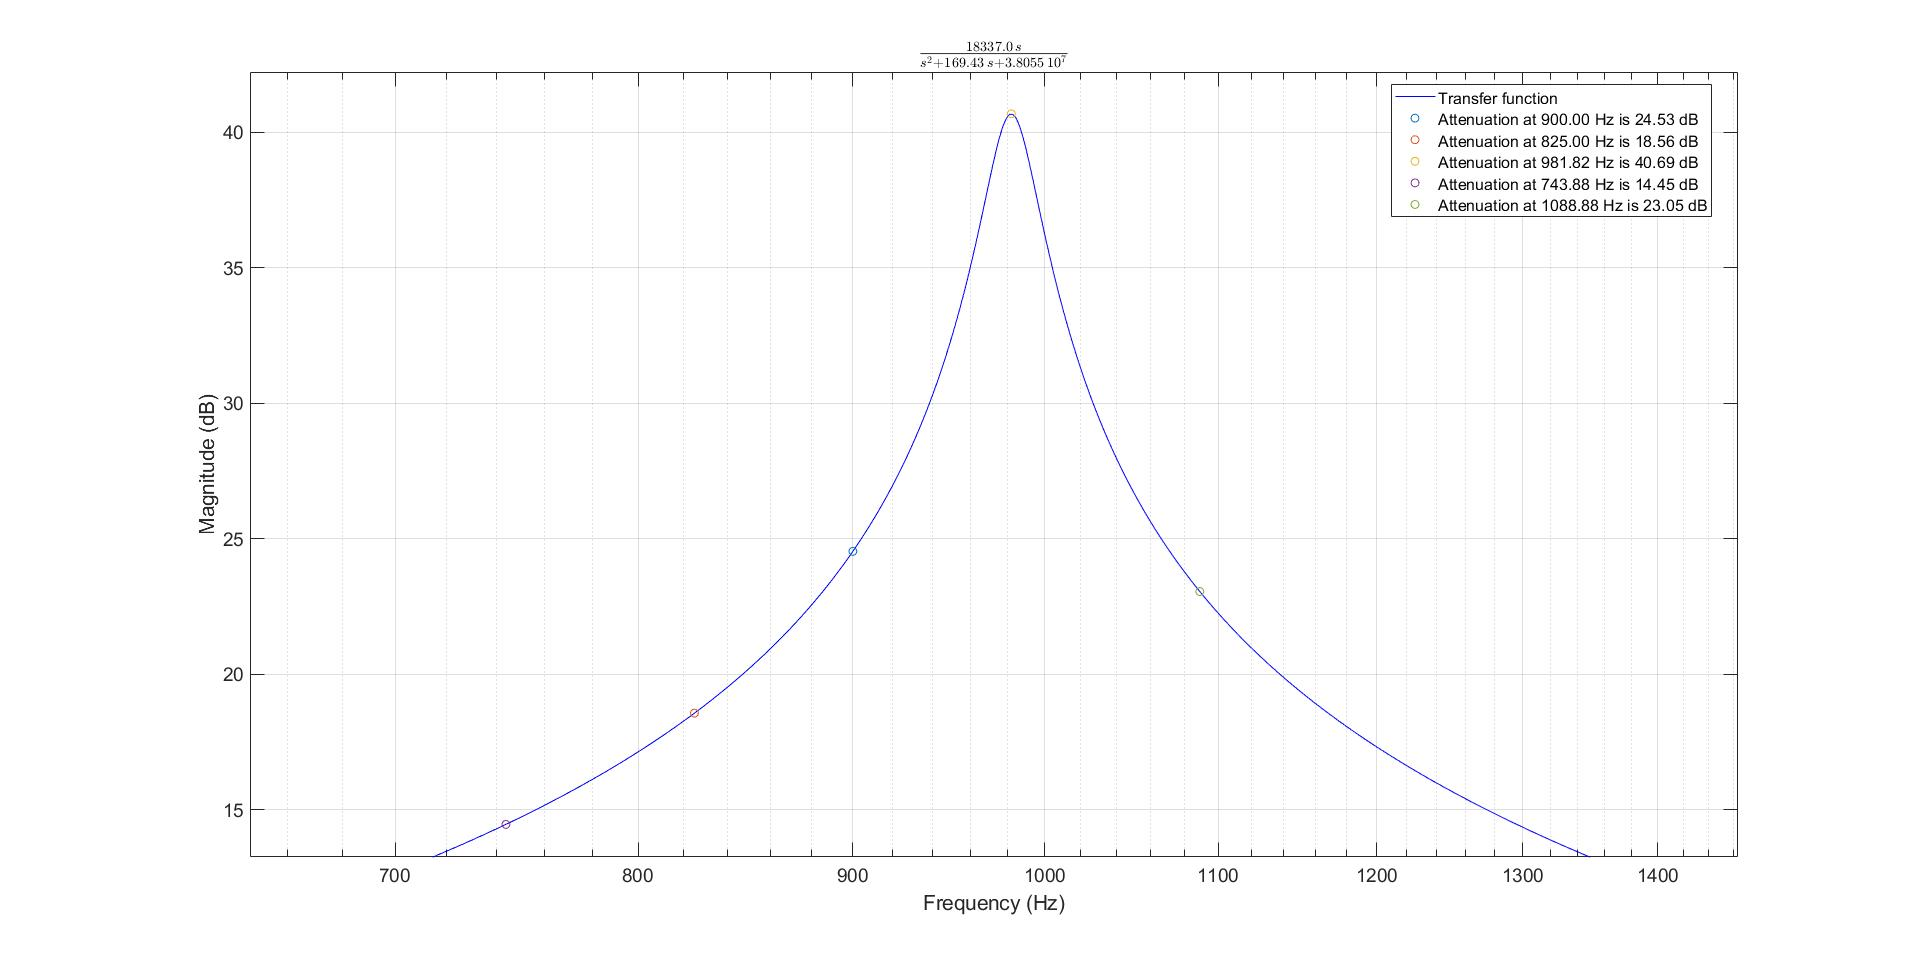
\includegraphics[width=120mm,scale=2]{thema2/z4.jpg}
\end{figure*}  
\newpage
\section*{Aπόκριση πλάτους της συνολικής συνάρτησης μεταφοράς} 
Παρακάτω βλέπουμε την απόκριση πλάτους της συνολικής συνάρτησης μεταφοράς του φίλτρου συναρτήσει της συχνότητας.
\begin{figure*}[h!]
\centering
 	\advance\leftskip-0.1cm
  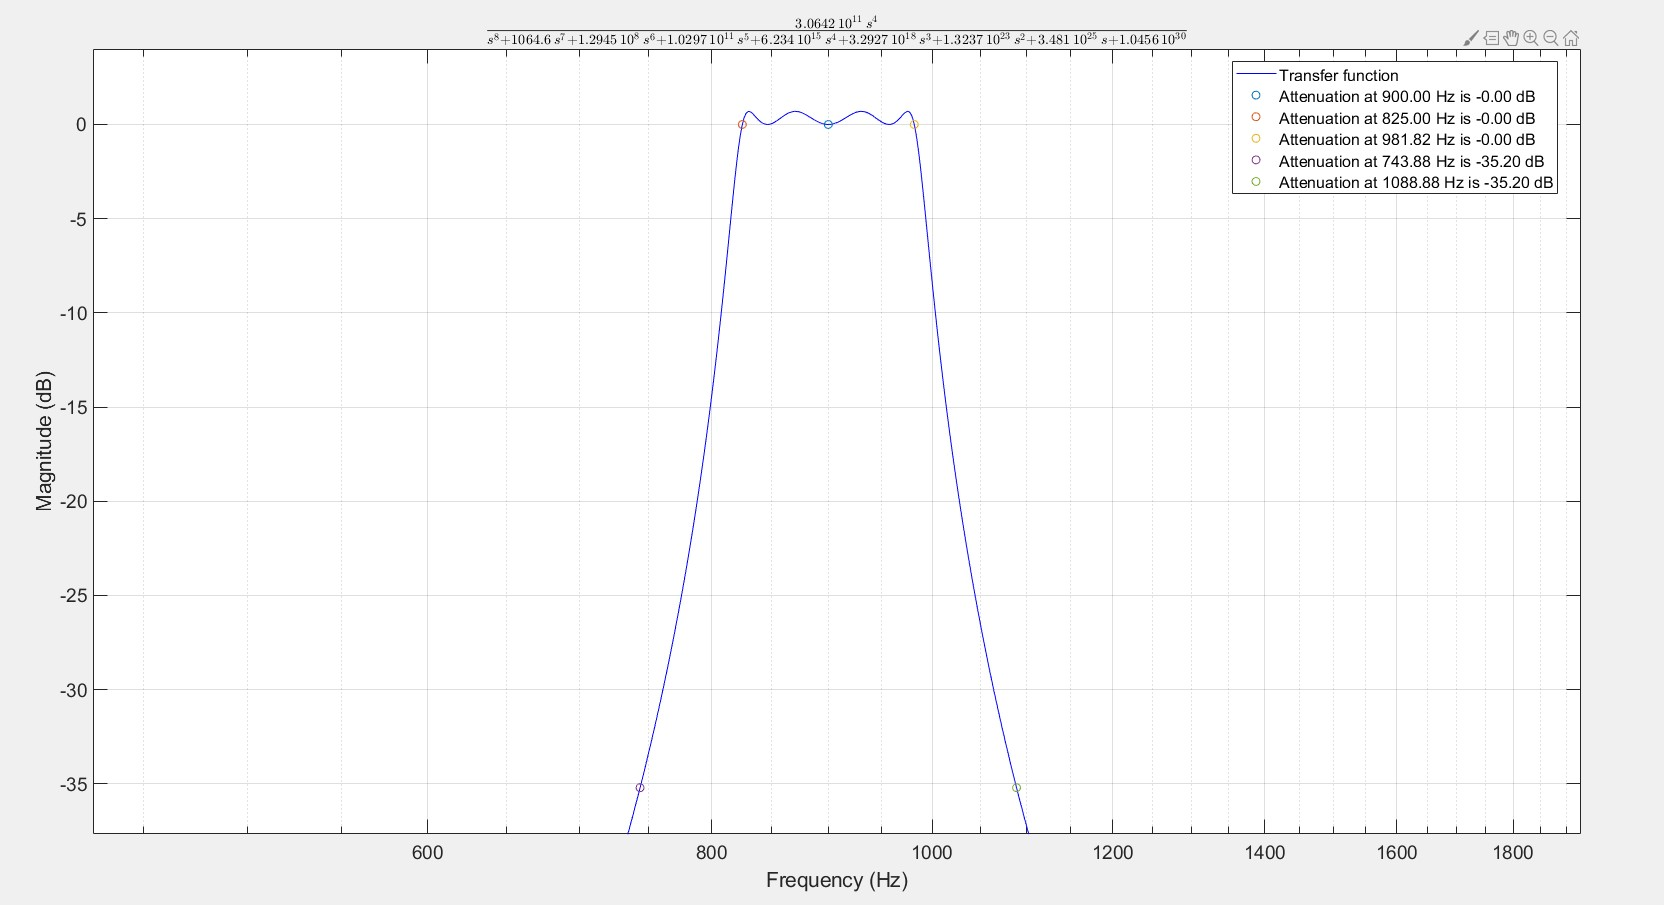
\includegraphics[width=120mm,scale=2]{thema2/matlab4.jpg}
\end{figure*}  \\
Στο παραπάνω διάγραμμα κανουμε ζουμ στην ζώνη διόδου και ελέγχουμε τις μεγιστες τιμες της κυμάτωσης ωστε να επιβεβαιώσουμε οτι πληρείται η προδιαγραφή $a_{max} =0.6944dB$ 
\begin{figure*}[h!]
\centering
 	\advance\leftskip-0.1cm
  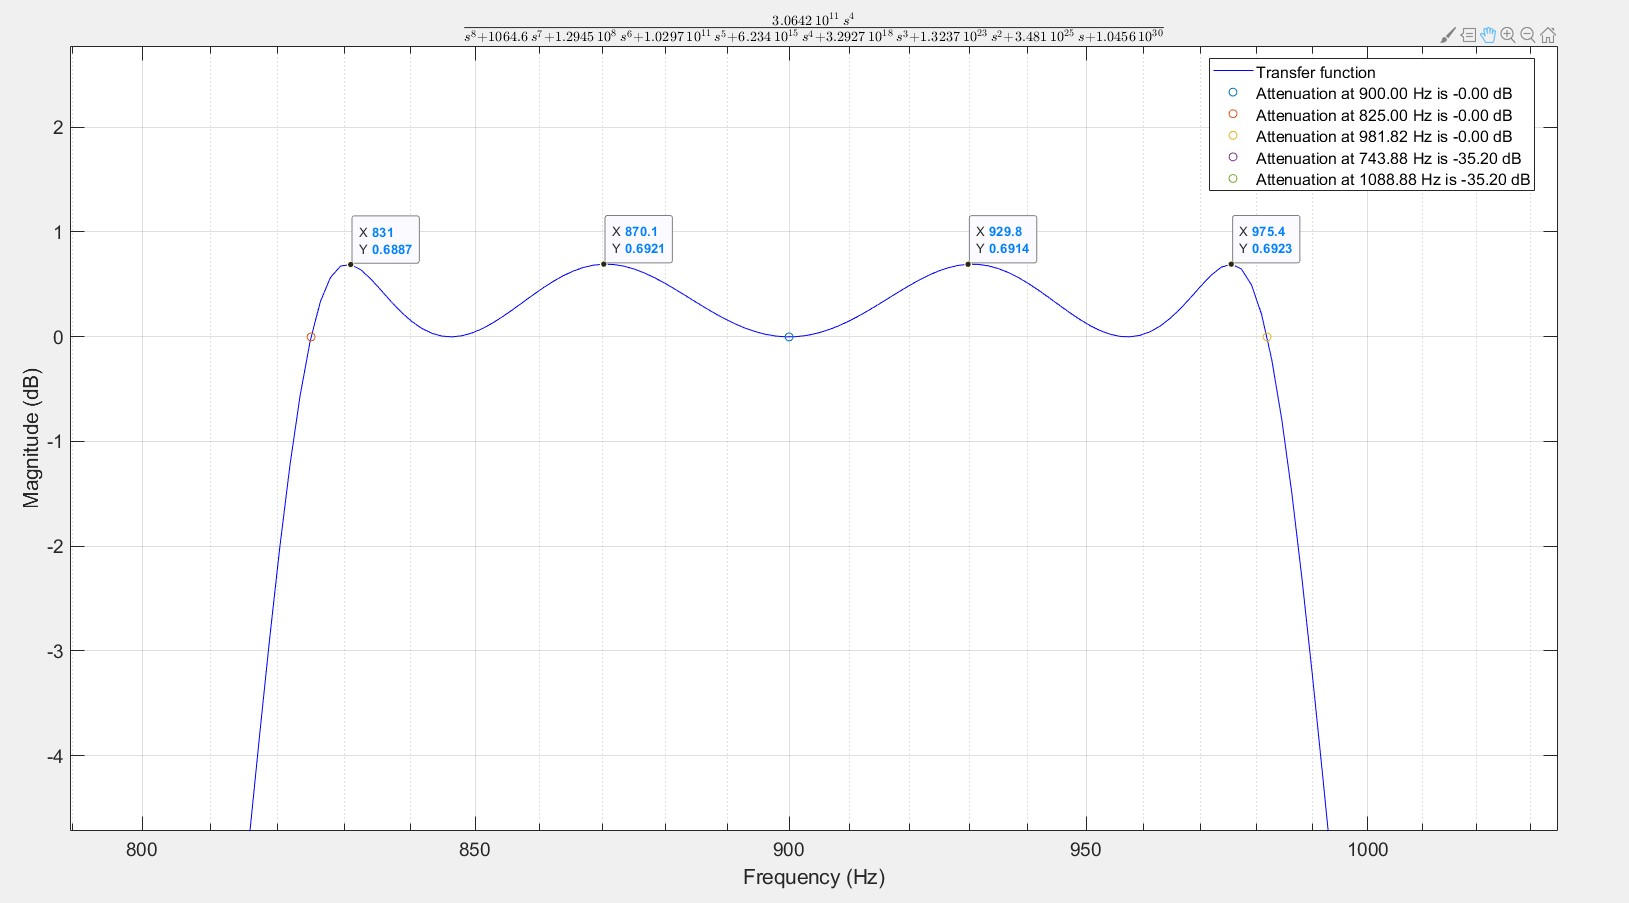
\includegraphics[width=120mm,scale=2]{thema2/matlab3a.jpg}
\end{figure*}
\newpage
\section*{Κοινό διάγραμμα αποκρίσεων} 
Σε αυτό το σημείο παραθέτουμε όλες τις παραπάνω αποκρίσεις σε ένα κοινό διάγραμμα Bode.
\begin{figure*}[h!]
\centering
 	\advance\leftskip-4cm
  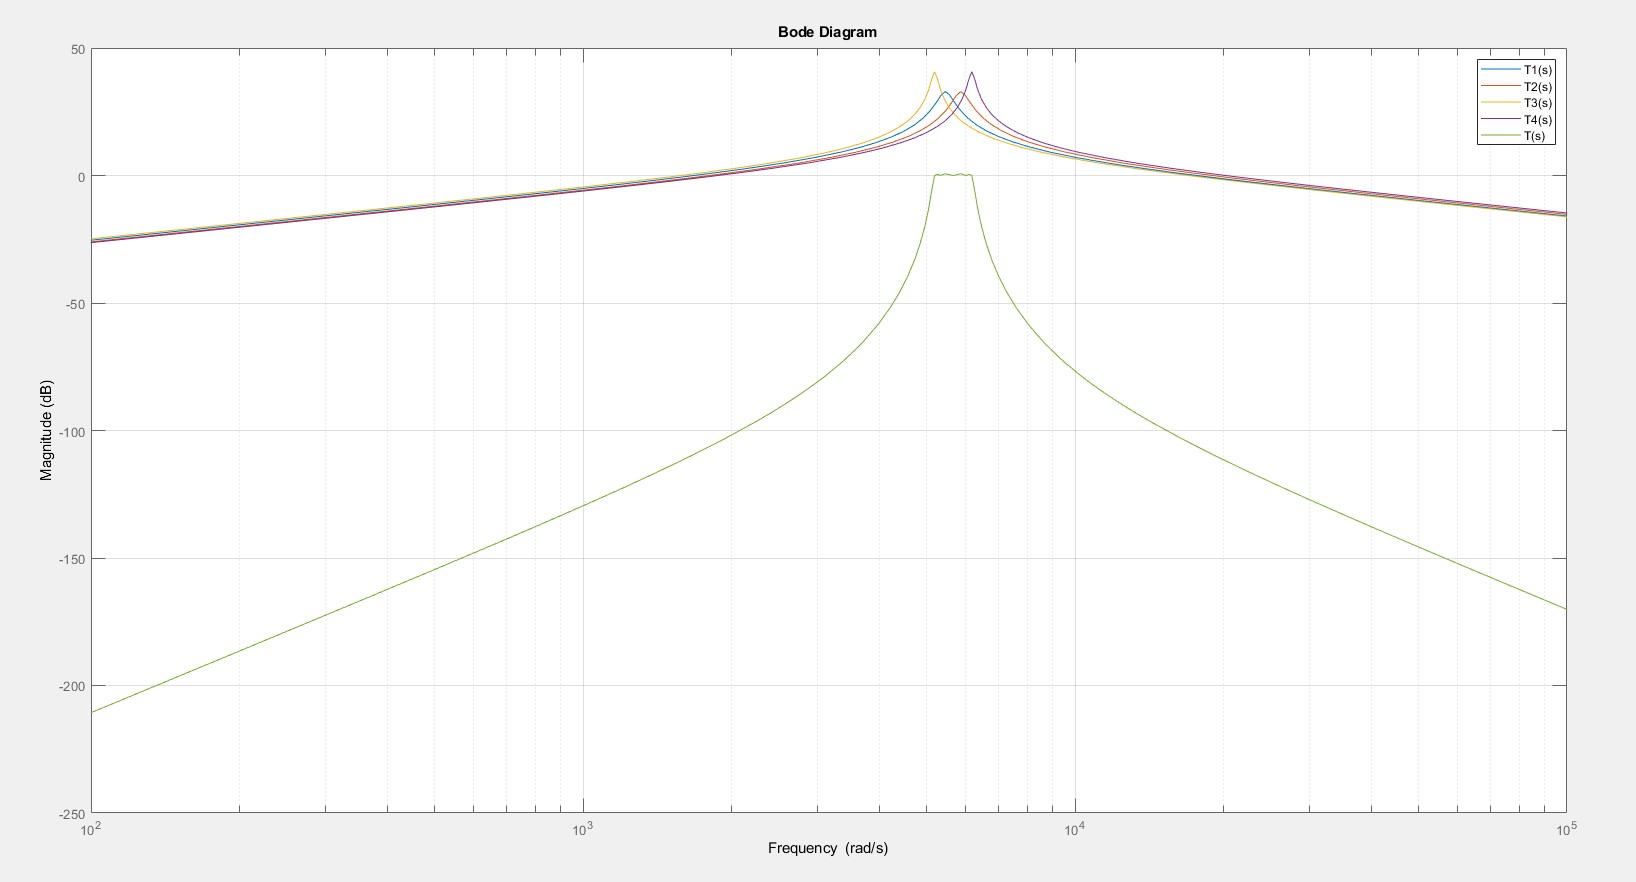
\includegraphics[width=200mm,scale=2]{thema2/matlab5.jpg}
\end{figure*}  

\newpage
\section*{Συνάρτηση απόσβεσης της συνολικής συνάρτησης μεταφοράς} 
Παρακάτω φαίνεται η συνάρτηση απόσβεσης σε dB της συνολικής συνάρτησης μεταφοράς συναρτήσει της συχνότητας. 
\begin{figure*}[h!]
\centering
 	\advance\leftskip-4.1cm
  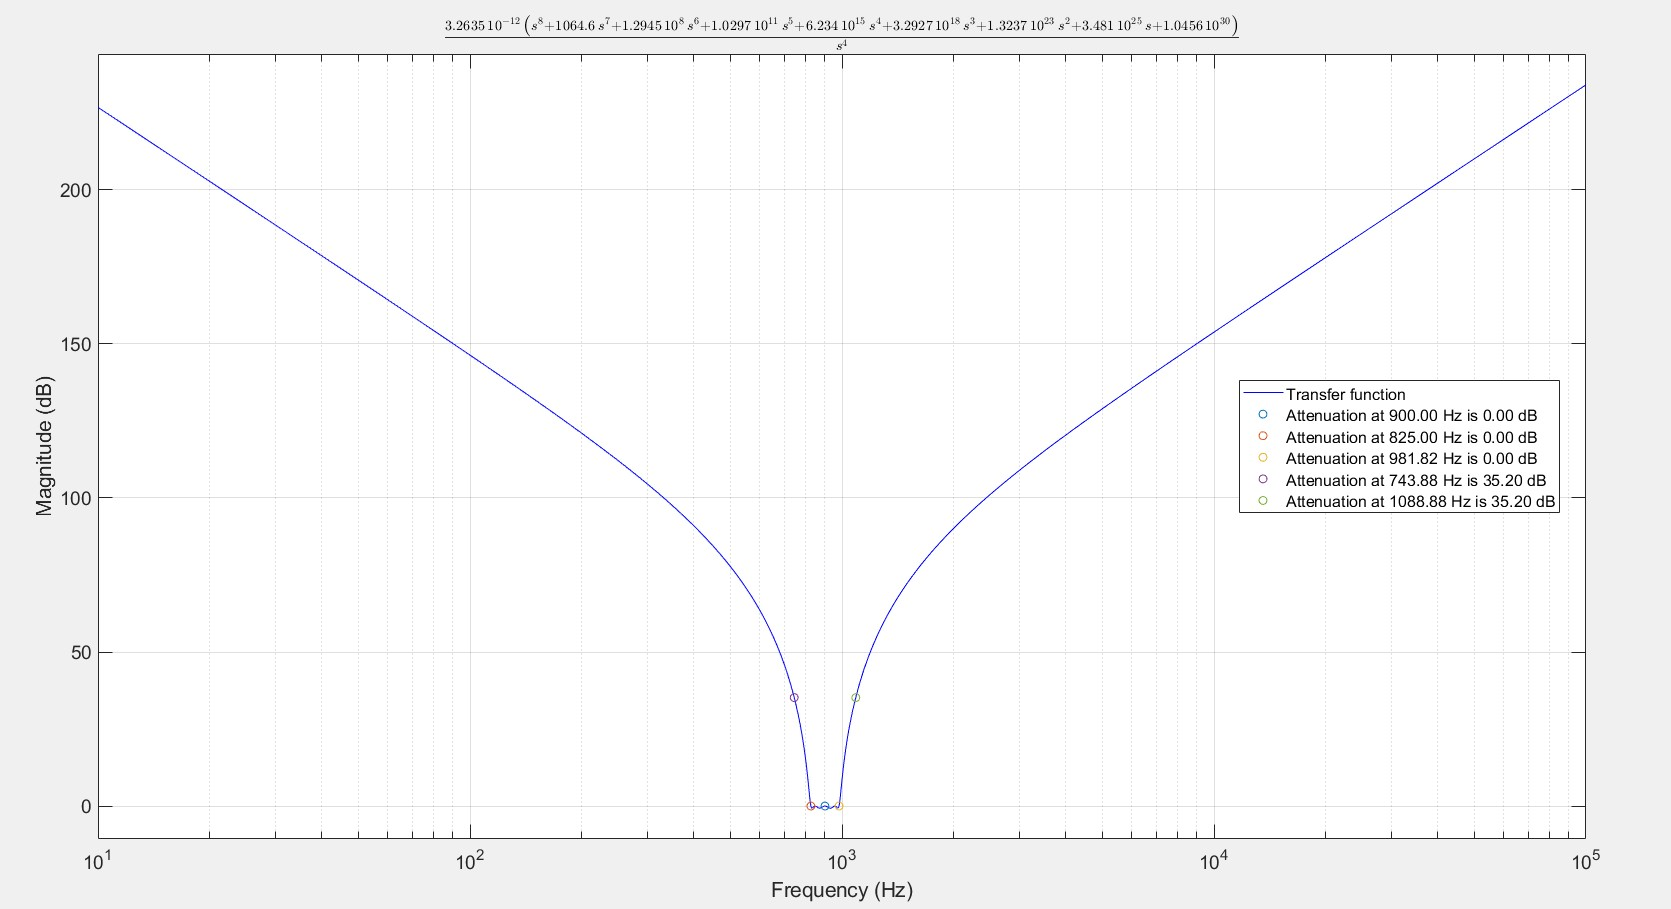
\includegraphics[width=205mm,scale=2]{thema2/matlab6.jpg}
\end{figure*}  
\\
    \color{black} Στη συνάρτηση  απόσβεσης σημειώνουμε τις κρίσιμες συχνότητες οι οποίες καθορίζουν την ζώνη διόδου και αποκοπής , δηλαδή τις $f_0$=900Ηz, $f_1$=825Hz, $f_2$=981.81Hz, $f_3$=743.88Hz, $f_4$=1088.88Hz, καθώς και τις αντίστοιχες αποσβέσεις.
\clearpage
Στο διάγραμμα που ακολουθεί σημειώνουμε αυτες τις αποσβέσεις που ακολουθούν ωστε να δείξουμε οτι οι μέγιστες τιμές της κυμάτωσης δεν ξεπερνάνε το οριο των προδιαγραφών $a_{max}$ εντός της ζώνης διόδου.
\begin{figure*}[h!]
\centering
 	\advance\leftskip-1.8cm
  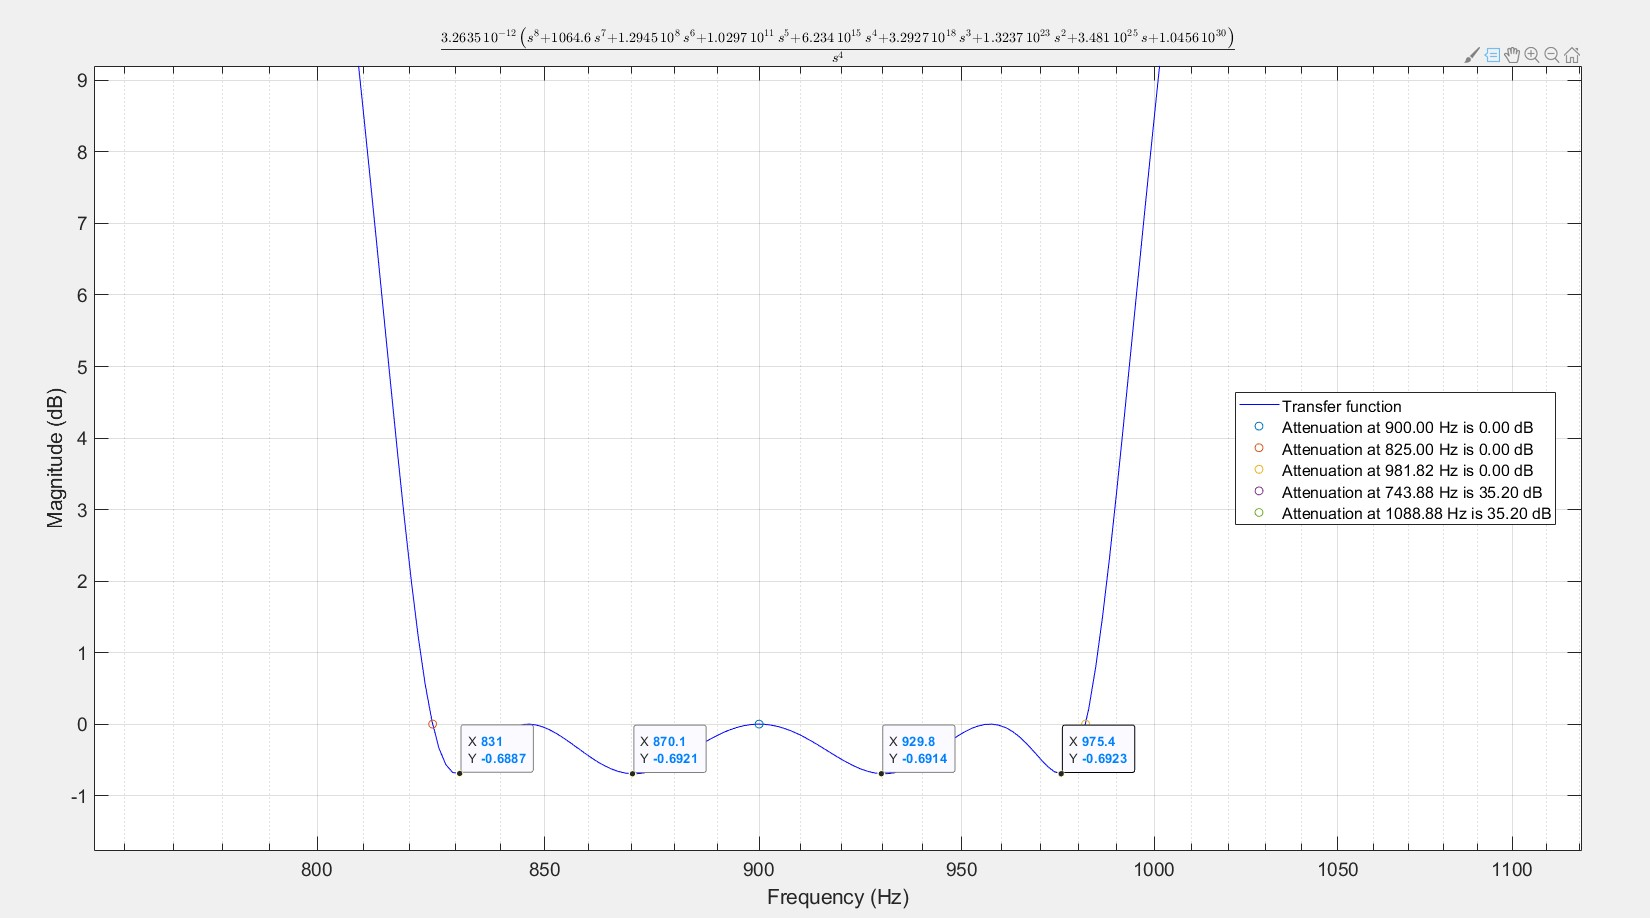
\includegraphics[width=170mm,scale=2]{thema2/matlab6a.jpg}
\end{figure*}\\
 Aπ το παραπάνω σχήμα διαπιστώνουμε οτι πληρούνται οι προδιαγραφές στην ζώνη διόδου καθως εχουμε απόσβεση μικρότερη της $a_{max}$= 0.6944 dB  και στην ζώνη αποκοπής μεγαλύτερης της $a_{min}$ = 29.611 dB δεδομένου οτι το κέρδος στην κεντρική συχνότητα είναι 0 dB.\\
\clearpage

\subsection*{Γ. Υλοποίηση του Κυκλώματος του Φίλτρου στο MULTISIM}
\addcontentsline{toc}{subsection}{Γ. Υλοποίηση του Κυκλώματος του Φίλτρου στο MULTISIM}

\large{}
Σχεδιάζουμε το κύκλωμα μας στο ElectronicWorkBench (MULTISIM) προκειμένου να ελέγξουμε αν υλοποιεί την συνολική συνάρτηση μεταφοράς που αναλύθηκε στο προηγούμενο στάδιο της εργασίας αλλά και για να διερευνήσουμε την απόκριση του φίλτρου όταν αυτό διεγείρεται από ένα στοιχειώδες περιοδικό σήμα.
Εισάγουμε λοιπόν όπως απαιτείται τις διάφορες στοιχειώδεις μονάδες του φίλτρου που έχουν σχεδιασθεί στην προηγούμενη φάση της εργασίας στο περιβάλλον MULTISIM και παίρνουμε το παρακάτω κύκλωμα.
\begin{figure*}[h!]
\centering
 	\advance\leftskip-3.5cm
  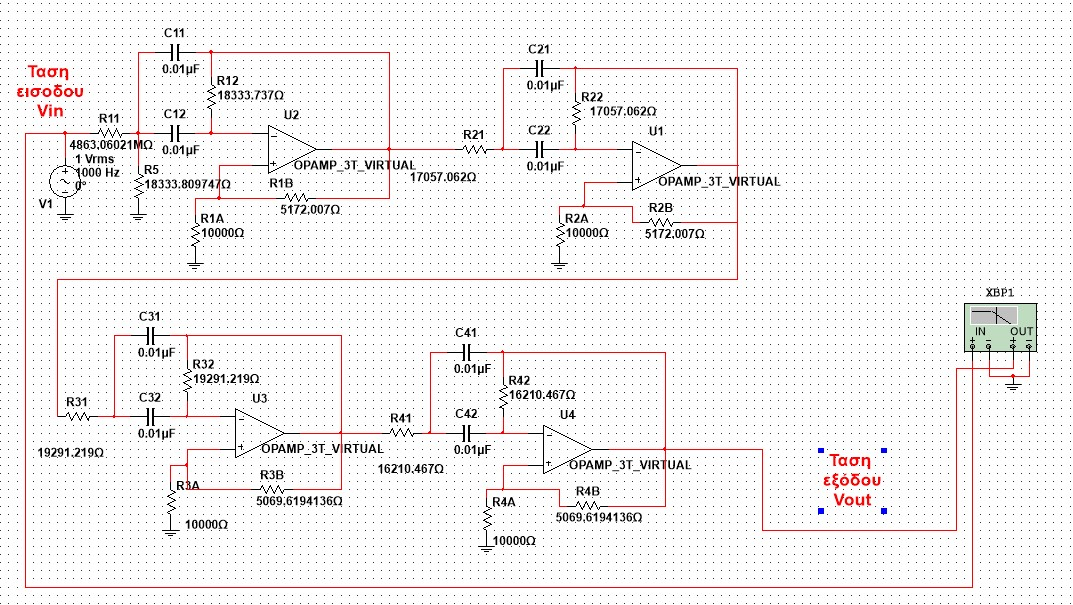
\includegraphics[width=190mm,scale=2]{thema2/multisim0.jpg}
\end{figure*} 
\clearpage
Στο κύκλωμα που έχουμε σχεδιάσει χρησιμοποιούμε τον Bode-Plotter για να προκύψει η απόκριση συχνότητας του φίλτρου-κυκλώματος. Το διάγραμμα που παίρνουμε φαίνεται παρακάτω δειχνει την απόσβεση στην κεντρική συχνότητα $f_0 = 900Hz$ :
\begin{figure*}[h!]
\centering
 	\advance\leftskip-1cm
  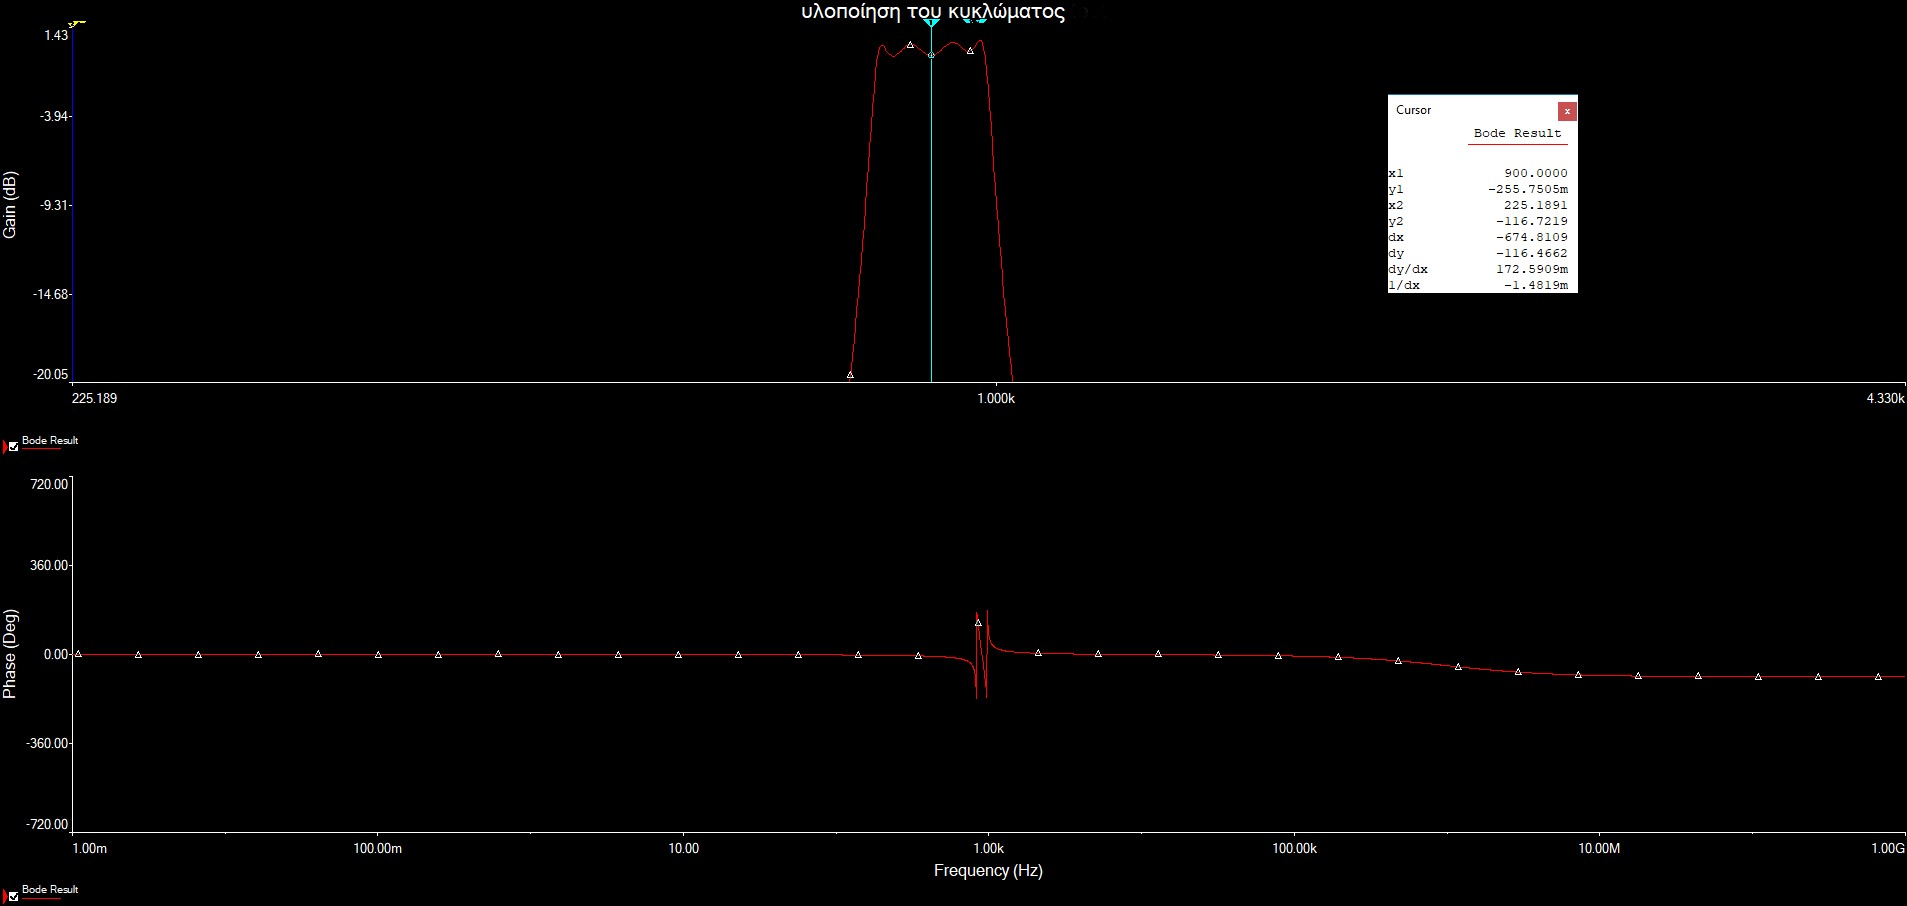
\includegraphics[width=130mm,scale=2]{thema2/multisim1.jpg}
\end{figure*} \\
Tο παρακάτω διάγραμμα του Multisim απεικονίζει ότι ακριβώς και το προηγούμενο αλλά με δυνατότητα ανάγνωσης των τιμών $f_1 = 825Hz$ και $f_2 = 981.82Hz$.
\begin{figure*}[h!]
\centering
 	\advance\leftskip-2cm
  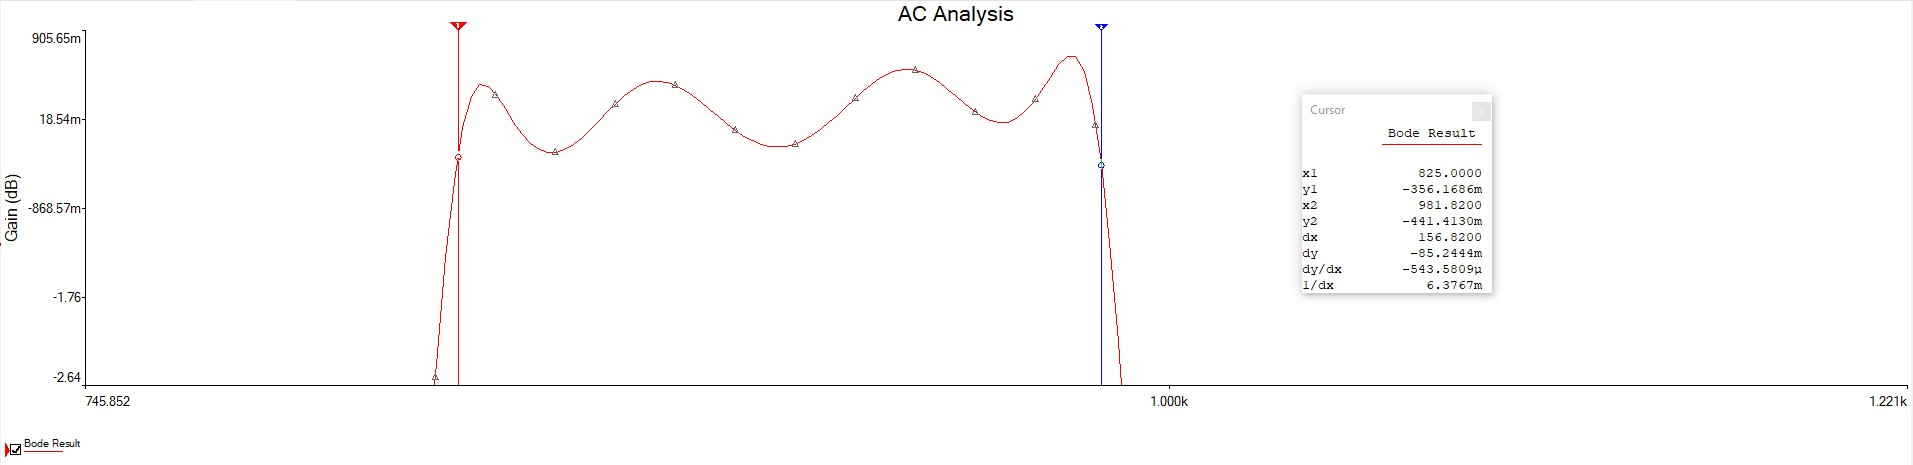
\includegraphics[width=150mm,scale=2]{thema2/multisim2a.jpg}
\end{figure*} \\
Η παραπάνω εικόνα μας δείχνει οτι η προδιαγραφή $a_{max} = 0.6944dB$ πληρείται. Στις συχνότητες $f_1 = 825Hz$ και $f_2 = 981.82Hz$ εχουμε αποσβέσεις 0,356dB και 0,441dB αντίστοιχα.
\clearpage
Θέλουμε εντος της ζώνης διόδου να μην έχουμε αποσβέσεις μεγαλύτερες απο την $a_{max}$. Για αυτό ακριβως τον λόγο ελεγχουμε την μέγιστη και την ελάχιστη τιμη της αποσβεσης εντός της ζώνης διόδου ώστε να δούμε αν  η $a_{max} = 0.6944dB$ πληρείται. Η παραπάνω εικόνα δείχνει οτι καμία συχνότητα στην ζώνη διόδου δε ξεπερνά την $a_{max}$ αφου η απόσβεση δε ξεπερνα τα 0.647 dB.}
\begin{figure*}[h!]
\centering
 	\advance\leftskip-1cm
  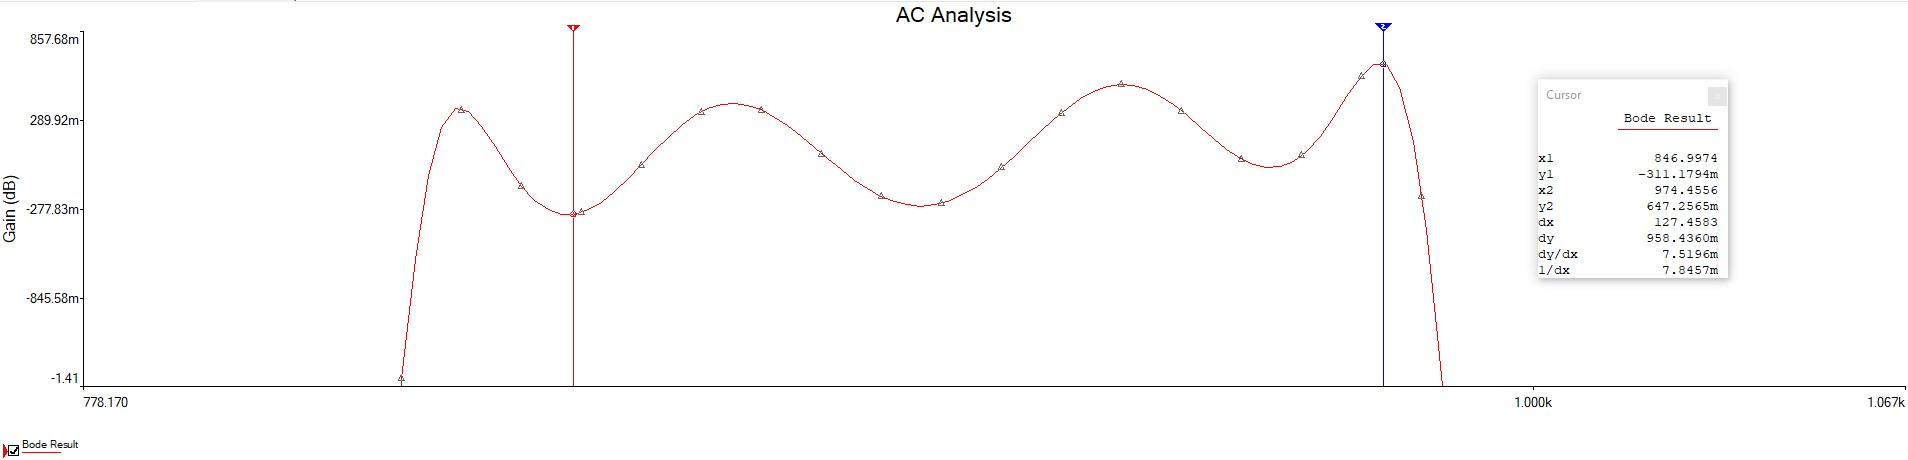
\includegraphics[width=140mm,scale=2]{thema2/multisim3a.jpg}
\end{figure*} 

Για τις συχνότητες $f_3 = 743.88Hz$ και $f_4 = 1088.88Hz$  η παρακάτω εικόνα μας δείχνει οτι η προδιαγραφή $a_{min} = 29.41 dB$ υπερπληρείται αφού  έχουμε αποσβέσεις 35,55dB και 35,71dB αντίστοιχα.

\begin{figure*}[h!]
\centering
 	\advance\leftskip-1cm
  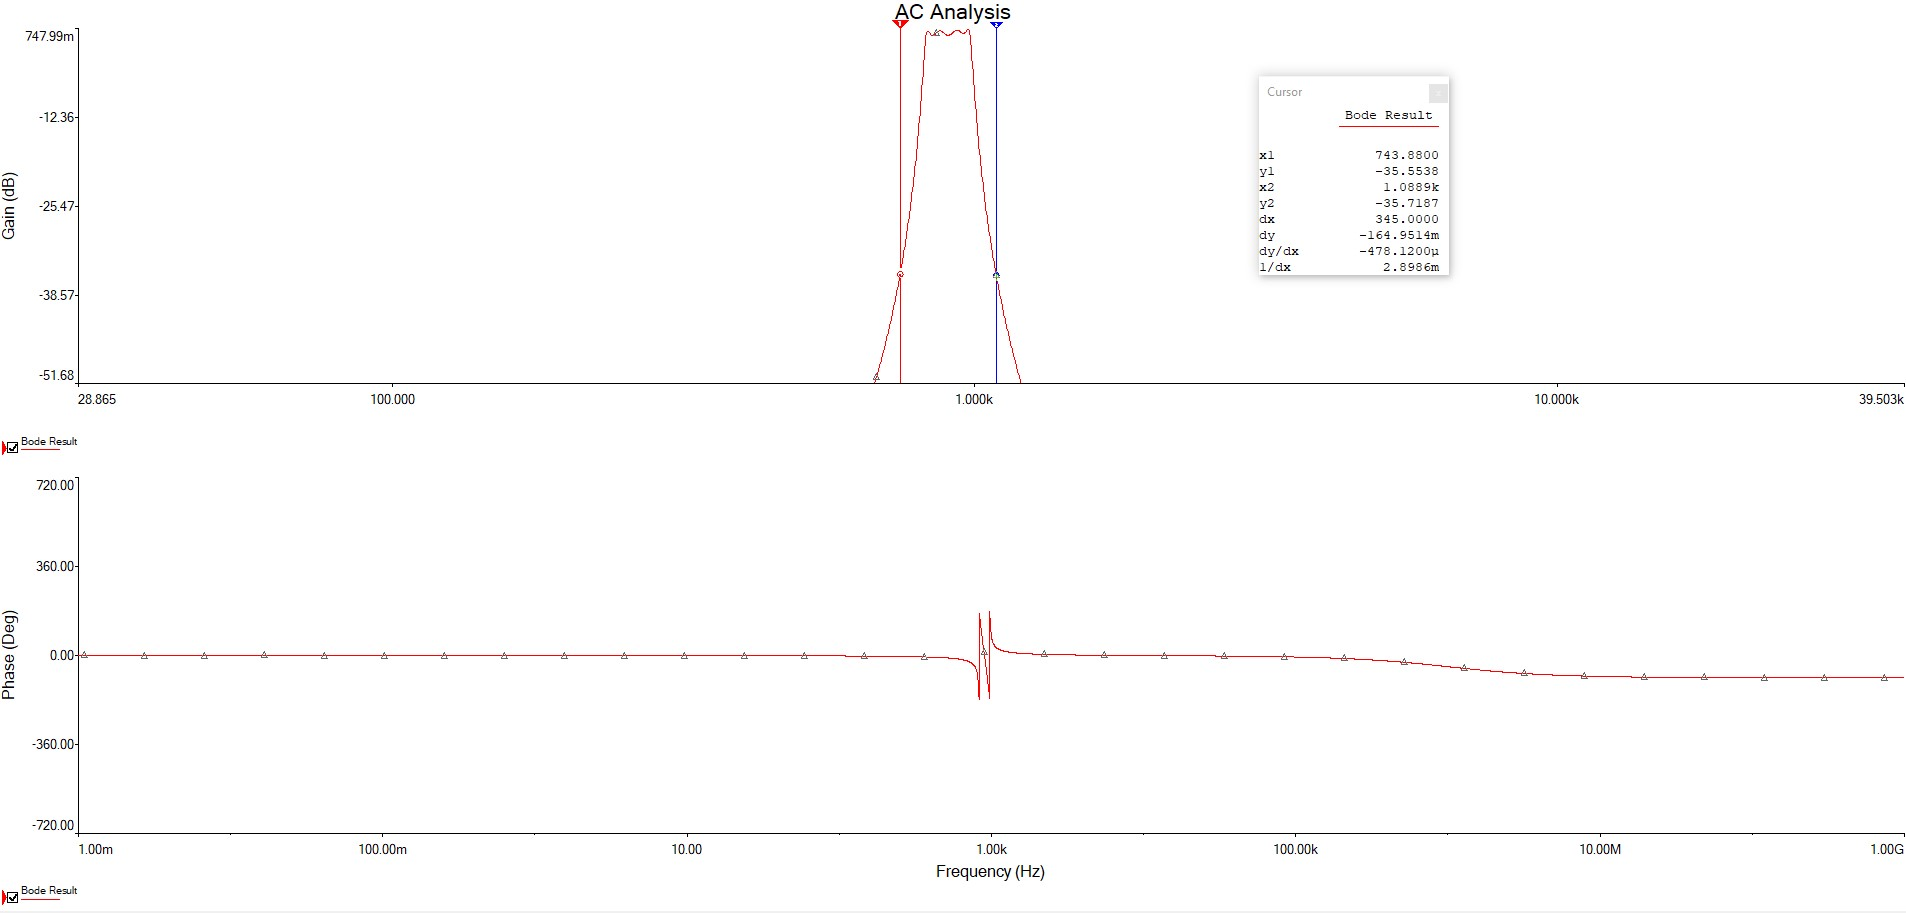
\includegraphics[width=150mm,scale=2]{thema2/matlab5a.jpg}
\end{figure*} 

\clearpage
Εισάγουμε τώρα στο κύκλωμα ενα περιοδικο σήμα\begin{changemargin}{-2.5cm}{0.5cm}\begin{equation*}
\boxed{
f(t) = cos(5419.24t) + 0.6 cos(11074.11t) + cos(2336.97t) + 0.8cos(16419.95t) + 0.4cos(23945.76t) }
\end{equation*}
\end{changemargin}
Με πλάτη 1 , 0.6 , 1 , 0.8 , 0.4 και συχνότητες  862.5 Hz , 1762.5 Hz , 372 Hz , 2613 Hz , 3811 Hz\\
Στην συνέχεια χρησιμοποιούμε έναν παλμογράφο στην είσοδο και την έξοδο και δημιουργούμε τα αντίστοιχα figures για το παραπάνω πείραμα.
\begin{figure*}[h!]
\centering
 	\advance\leftskip-4cm
  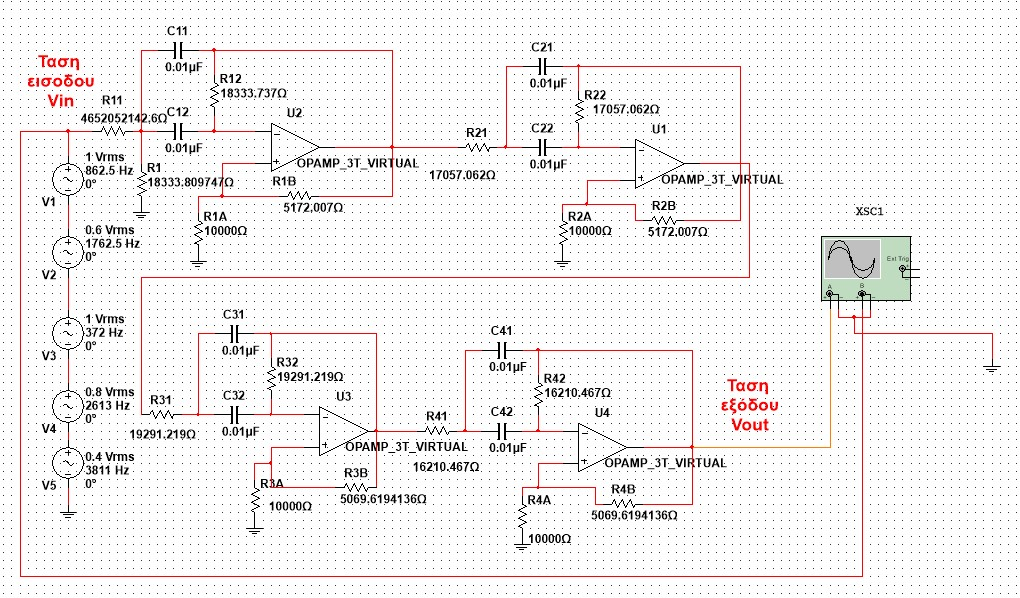
\includegraphics[width=200mm,scale=2]{thema2/multisim5.jpg}
\end{figure*} 
\clearpage
\textbf{\underline{Σήμα Εισόδου (Εικόνα παλμογράφου):}}
\begin{figure*}[h!]
\centering
 	\advance\leftskip-1cm
  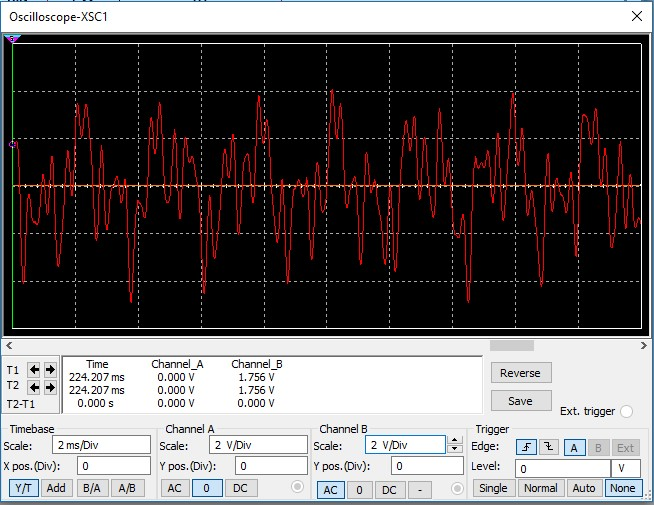
\includegraphics[width=130mm,scale=2]{thema2/multisim6.jpg}
\end{figure*} \\
\textbf{\underline{Transient Analysis σηματος ειδόσου (ασπρο φόντο):}}
\begin{figure*}[h!]
\centering
 	\advance\leftskip-1cm
  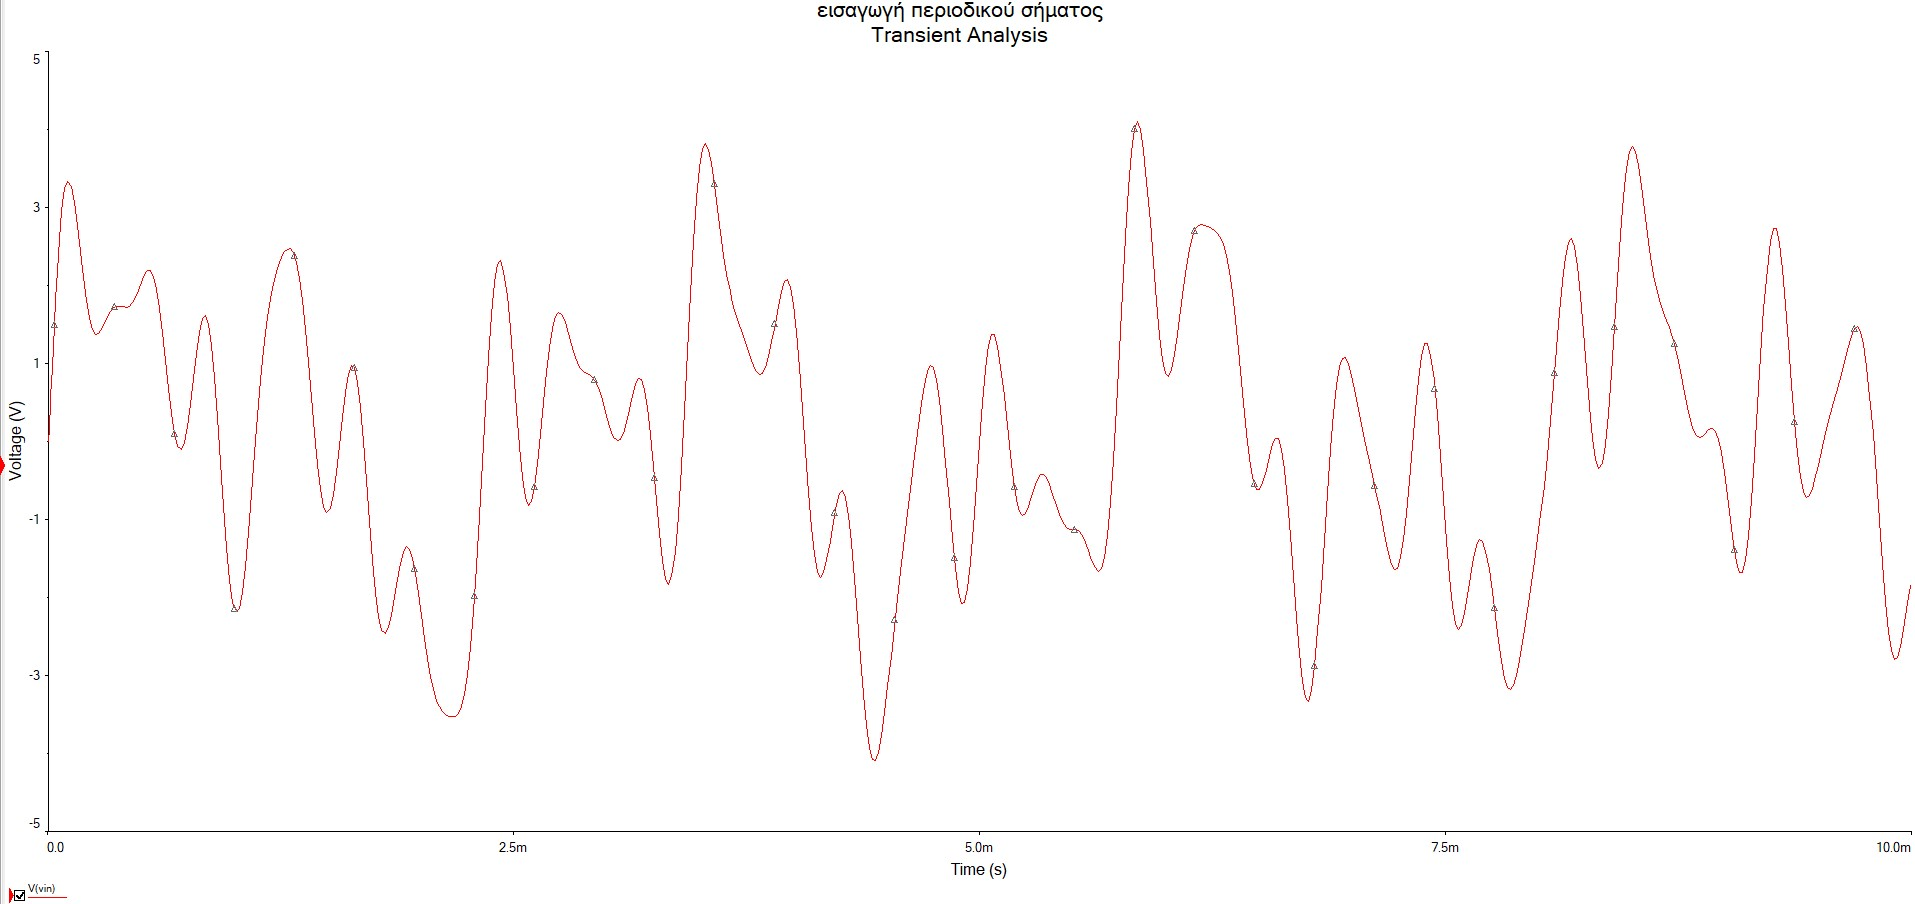
\includegraphics[width=130mm,scale=2]{thema2/multisim7.jpg}
\end{figure*} 
\clearpage
\textbf{\underline{Σήμα Εξόδου (Εικόνα παλμογράφου):}}
\begin{figure*}[h!]
\centering
 	\advance\leftskip-1cm
  \includegraphics[width=130mm,scale=2]{thema2/multisim8.jpg}
\end{figure*} \\
\textbf{\underline{Transient Analysis σηματος εξόδου (ασπρο φόντο):}}
\begin{figure*}[h!]
\centering
 	\advance\leftskip-2cm
  \includegraphics[width=130mm,scale=2]{thema2/multisim9.jpg}
\end{figure*} 
 \clearpage
 \textbf{\underline{Σήμα Εισόδου-Εξόδου (Εικόνα παλμογράφου):}} 
 \\[1.4\baselineskip]
 Το διάγραμμα που ακολουθεί περιλαμβάνει  σήμα εξόδου (πράσινο χρωμα) και το σήμα ειδόδου (μπλέ χρώμα) στα channel του παλμογράφου Α και Β αντίστοιχα.  \\[0.4\baselineskip]
 \begin{figure*}[h!]
\centering
 	\advance\leftskip-0.7cm
  \includegraphics[width=140mm,scale=2]{thema2/multisim10.jpg}
\end{figure*}   \\[1.4\baselineskip]
Στα παραπάνω διαγράμματα μπορούμε να δούμε αναλυτικά τα σήματα εισόδου (channel b) και εξόδου (channel a) σε κάθε σχήμα φαίνονται οι επιλογές που κάναμε στον παλμογράφο για να προκύψουν οι αντίστοιχες παραστάσεις (για παράδειγμα: V/Div ,  sec/Div κτλ.).
Πιο αναλυτικά, παρατηρούμε ότι το σήμα εξόδου είναι ίσο σε πλάτος σε σχέση με το σήμα εισόδου. Το κέρδος του φίλτρου γίνεται φανερό, καθώς το σήμα εξόδου εχει 0dB ενίσχυση. 
\clearpage
\subsection*{Σύκριση matlab-multisim}
\large{}
Σε αυτό το σημείο της άσκησης θέλουμε να δημιουργήσουμε τα φάσματα εισόδου και εξόδου του φίλτρου, Chebyshev. Για να γίνει κάτι τέτοιο θα εξετάσουμε τα φάσματα τόσο στο Multisim όσο και στο Matlab. Εφόσον μιλάμε για τα ίδια σήματα καθώς και για το ίδιο φίλτρο, αναμένουμε να έχουμε τα ίδια αποτελέσματα. \\[0.4\baselineskip]
Κατά συνέπεια, στην επόμενη σελίδα παρουσιάζουμε τα φάσματα FOURIER που προέρχονται από την FFT και τα οποία θα σχολιάσουμε στην συνέχεια.
\subsection*{Σχολιασμός εισόδου}
Γνωρίζουμε πως η είσοδος είναι ενα άθροισμα συνημιτόνων:
\begin{changemargin}{-2.5cm}{0cm}\begin{equation*}
\boxed{f(t) = cos(5419.24t) + 0.6 cos(11074.11t) + cos(2336.97t) + 0.8cos(16419.95t) + 0.4cos(23945.76t) }
\end{equation*}
\end{changemargin}
 το οποίο αν το μετασχηματίσεις στην συχνότητα θα γίνει αθροισμα dirac στις αντιστοιχες συχνότητες αφου ισχύει:
\begin{equation*}
\boxed{
Fourier-Transform \{cos(2πft)\} = π * [δ(ω-2πf) + δ(ω+2πf)]}
\end{equation*}
Αρα αναμένουμε το σήμα είσοδου στην συχνότητα να είναι ένα αθροισμα ώσεων στις συχνότητες  862.5 Hz , 1762.5 Hz , 372 Hz , 2613 Hz , 3811 Hz με τα αντίστοιχα πλάτη 1 , 0.6 , 1 , 0.8 , 0.4 
\subsection*{Σχολιασμός εξόδου}
Το ζωνοδιαβατό φίλτρο που κατασκευάζουμε εχει ζώνη διάβασης απο $f_1 = 825Hz$ μέχρι $f_2 = 981.82Hz$ αρα αναμένουμε απο τις συχνότητες εισόδου:  862.5 Hz , 1762.5 Hz , 372 Hz , 2613 Hz , 3811 Hz να περάσει μόνο η 862,5Hz και η άλλες να αποκοπούν. Για αυτό οπως είδαμε παραπάνω η έξοδος μας ήταν ημιτονοειδής μορφής.
\clearpage
\textbf{\underline{Σήμα Εισόδου (Fourier) - MATLAB:}}
\begin{figure*}[h!]
\centering
 	\advance\leftskip-0.5cm
  \includegraphics[width=130mm,scale=2]{thema2/fmatin.jpg}
\end{figure*} \\[1.4\baselineskip]
\textbf{\underline{Σήμα Εξόδου (Fourier) - MATLAB:}}
\begin{figure*}[h!]
\centering
 	\advance\leftskip-0.5cm
  \includegraphics[width=130mm,scale=2]{thema2/fmatout.jpg}
\end{figure*} \\
Βλέπουμε πως τα αποτελέσματα είναι τα ίδια με τα αναμενόμενα που σχολιάσαμε παραπάνω στις παραγράφους\textbf{ Σχολιασμός εισόδου , Σχολιασμος εξόδου}
\clearpage
\textbf{\underline{Σήμα Εισόδου (Fourier) - MULTISIM:}}
\begin{figure*}[h!]
\centering
 	\advance\leftskip-0.5cm
  \includegraphics[width=130mm,scale=2]{thema2/fmulin.jpg}
\end{figure*}  \\[1.4\baselineskip]
\textbf{\underline{Σήμα Εξόδου (Fourier) - MULTISIM:}}
\begin{figure*}[h!]
\centering
 	\advance\leftskip-0.5cm
  \includegraphics[width=130mm,scale=2]{thema2/fmulout.jpg}
\end{figure*} \\
\normalsize{}
Στο διάστημα από $f_1$=825Ηz μέχρι $f_2$=1088,88hz παρατηρώ ότι οι αρμονικές
μου περνάνε κανονικά. Αντίστοιχα κάτω από $f_3$=743Hz και πάνω από
$f_4$=1088.88Khz βρίσκομαι στην ζώνη αποκοπής οπότε έχω πολύ μεγάλη απόσβεση και το φίλτρο μου κόβει τις αρμονικές μου. Συνεπώς στην έξοδο οι αρμονικές οι οποίες βλέπω περα των συχνοτήτων $f_1=825Hz < f < f_2 = 981.82Hz$
είναι πολύ μικρότερου πλάτους.
Έτσι συνάγεται το συμπέρασμα ότι το φίλτρο λειτουργεί σωστά.Έχουμε κατασκευάσει δηλαδή ένα ζωνοπερατό φίλτρο.
\large{}
\clearpage



































































































%%%%%%%
%%%%%%%
%%%%%%%
%%%%%%%
%%%%%%%
%%%%%%%
%%%%%%%
%%%%%%%
%%%%%%%
%%%%%%%
%%%%%%%
%%%%%%%
%%%%%%%
%%%%%%%
%%%%%%%
%%%%%%%
%%%%%%%
%%%%%%%
%%%%%%%
%%%%%%%
%%%%%%%
%%%%%%%
%%%%%%%
%%%%%%%
%%%%%%%
%%%%%%%
%%%%%%%
%%%%%%%
%%%%%%%
%%%%%%%
%%%%%%%
%%%%%%%
%%%%%%%
%%%%%%%
%%%%%%%
%%%%%%%
%%%%%%%
%%%%%%%
%%%%%%%
%%%%%%%
%%%%%%%
%%%%%%%
%%%%%%%
%%%%%%%
%%%%%%%
%%%%%%%
%%%%%%%
%%%%%%%
%%%%%%%
%%%%%%%
%%%%%%%
%%%%%%%
%%%%%%%
%%%%%%%
%%%%%%%
%%%%%%%
%%%%%%%
%%%%%%%
%%%%%%%
%%%%%%%
%%%%%%%
%%%%%%%
%%%%%%%
%%%%%%%
%%%%%%%
%%%%%%%
%%%%%%%
%%%%%%%
%%%%%%%
%%%%%%%
%%%%%%%
%%%%%%%
%%%%%%%
%%%%%%%
%%%%%%%
%%%%%%%
%%%%%%%
%%%%%%%
%%%%%%%
%%%%%%%
%%%%%%%
%%%%%%%
%%%%%%%
%%%%%%%
%%%%%%%
%%%%%%%
%%%%%%%
%%%%%%%
%%%%%%%
%%%%%%%
%%%%%%%
%%%%%%%
%%%%%%%
%%%%%%%
%%%%%%%
%%%%%%%
%%%%%%%
%%%%%%%
%%%%%%%
%%%%%%%
%%%%%%%
%%%%%%%
%%%%%%%
%%%%%%%
%%%%%%%
%%%%%%%
%%%%%%%
%%%%%%%
%%%%%%%
%%%%%%%
%%%%%%%
%%%%%%%
%%%%%%%
%%%%%%%
%%%%%%%
%%%%%%%
%%%%%%%
%%%%%%%
%%%%%%%
%%%%%%%
%%%%%%%
%%%%%%%
%%%%%%%
%%%%%%%
%%%%%%%
%%%%%%%
%%%%%%%
%%%%%%%
%%%%%%%
%%%%%%%
%%%%%%%
%%%%%%%
%%%%%%%
%%%%%%%
%%%%%%%
%%%%%%%
%%%%%%%
%%%%%%%
%%%%%%%
%%%%%%%
%%%%%%%
%%%%%%%
%%%%%%%
%%%%%%%
%%%%%%%
%%%%%%%
%%%%%%%
%%%%%%%
%%%%%%%
%%%%%%%
%%%%%%%
%%%%%%%
%%%%%%%
%%%%%%%
%%%%%%%
%%%%%%%
%%%%%%%
%%%%%%%
%%%%%%%
%%%%%%%
%%%%%%%
%%%%%%%
%%%%%%%
%%%%%%%
%%%%%%%
%%%%%%%
%%%%%%%
%%%%%%%
%%%%%%%
%%%%%%%
%%%%%%%
%%%%%%%
%%%%%%%
%%%%%%%
%%%%%%%
%%%%%%%
%%%%%%%
%%%%%%%
%%%%%%%
%%%%%%%
%%%%%%%
%%%%%%%
%%%%%%%
%%%%%%%
%%%%%%%
%%%%%%%
%%%%%%%
%%%%%%%
%%%%%%%
%%%%%%%
%%%%%%%
%%%%%%%
%%%%%%%
%%%%%%%
%%%%%%%
%%%%%%%
%%%%%%%
%%%%%%%
%%%%%%%
%%%%%%%
%%%%%%%
%%%%%%%
%%%%%%%
%%%%%%%
%%%%%%%
%%%%%%%
%%%%%%%
%%%%%%%
%%%%%%%
%%%%%%%
%%%%%%%
%%%%%%%
%%%%%%%
%%%%%%%
%%%%%%%
%%%%%%%
%%%%%%%
%%%%%%%
%%%%%%%
%%%%%%%
%%%%%%%
%%%%%%%
%%%%%%%
%%%%%%%
%%%%%%%
%%%%%%%
%%%%%%%
%%%%%%%
%%%%%%%
%%%%%%%
%%%%%%%
%%%%%%%
%%%%%%%
%%%%%%%
%%%%%%%
%%%%%%%
%%%%%%%
%%%%%%%
%%%%%%%
%%%%%%%
%%%%%%%
%%%%%%%
%%%%%%%
%%%%%%%
%%%%%%%
%%%%%%%
%%%%%%%
%%%%%%%
%%%%%%%
%%%%%%%
%%%%%%%
%%%%%%%
%%%%%%%
%%%%%%%
%%%%%%%
%%%%%%%
%%%%%%%
%%%%%%%
%%%%%%%
%%%%%%%
%%%%%%%
%%%%%%%
%%%%%%%
%%%%%%%
%%%%%%%
%%%%%%%
%%%%%%%
%%%%%%%
%%%%%%%
%%%%%%%
%%%%%%%
%%%%%%%
%%%%%%%
%%%%%%%
%%%%%%%
%%%%%%%
%%%%%%%
%%%%%%%
%%%%%%%
%%%%%%%
%%%%%%%
%%%%%%%
%%%%%%%
%%%%%%%
%%%%%%%
%%%%%%%
%%%%%%%
%%%%%%%
%%%%%%%
%%%%%%%
%%%%%%%
%%%%%%%
%%%%%%%
%%%%%%%
%%%%%%%
%%%%%%%
%%%%%%%
%%%%%%%
%%%%%%%
%%%%%%%
%%%%%%%
%%%%%%%
%%%%%%%
%%%%%%%
%%%%%%%
%%%%%%%
%%%%%%%
%%%%%%%
%%%%%%%
%%%%%%%
%%%%%%%
%%%%%%%
%%%%%%%
%%%%%%%
%%%%%%%
%%%%%%%
%%%%%%%
%%%%%%%
%%%%%%%
%%%%%%%
%%%%%%%
%%%%%%%
%%%%%%%
%%%%%%%
%%%%%%%
%%%%%%%
%%%%%%%
%%%%%%%
%%%%%%%
%%%%%%%
%%%%%%%
%%%%%%%
%%%%%%%
%%%%%%%
%%%%%%%
%%%%%%%
%%%%%%%
%%%%%%%
%%%%%%%
%%%%%%%
%%%%%%%
%%%%%%%
%%%%%%%
%%%%%%%
%%%%%%%
%%%%%%%
%%%%%%%
%%%%%%%
%%%%%%%
%%%%%%%
%%%%%%%
%%%%%%%
%%%%%%%
%%%%%%%
%%%%%%%
%%%%%%%
%%%%%%%
%%%%%%%
%%%%%%%
%%%%%%%
%%%%%%%
%%%%%%%
%%%%%%%
%%%%%%%
%%%%%%%
%%%%%%%
%%%%%%%
%%%%%%%
%%%%%%%
%%%%%%%
%%%%%%%
%%%%%%%
%%%%%%%
%%%%%%%
%%%%%%%
%%%%%%%
%%%%%%%
%%%%%%%
%%%%%%%
%%%%%%%
%%%%%%%
%%%%%%%
%%%%%%%
%%%%%%%
%%%%%%%
%%%%%%%
%%%%%%%
%%%%%%%
%%%%%%%
%%%%%%%
%%%%%%%
%%%%%%%
%%%%%%%
%%%%%%%
%%%%%%%
%%%%%%%
%%%%%%%
%%%%%%%
%%%%%%%
%%%%%%%
%%%%%%%
%%%%%%%
%%%%%%%
%%%%%%%
%%%%%%%
%%%%%%%
%%%%%%%
%%%%%%%
%%%%%%%
%%%%%%%
%%%%%%%
%%%%%%%
%%%%%%%
%%%%%%%
%%%%%%%
%%%%%%%
%%%%%%%
%%%%%%%
%%%%%%%
%%%%%%%
%%%%%%%
%%%%%%%
%%%%%%%
%%%%%%%
%%%%%%%
%%%%%%%
%%%%%%%
%%%%%%%
%%%%%%%
%%%%%%%
%%%%%%%
%%%%%%%
%%%%%%%
%%%%%%%
%%%%%%%
%%%%%%%
%%%%%%%
%%%%%%%
%%%%%%%
%%%%%%%
%%%%%%%
%%%%%%%
%%%%%%%
%%%%%%%
%%%%%%%
%%%%%%%
%%%%%%%
%%%%%%%
%%%%%%%
%%%%%%%
%%%%%%%
%%%%%%%
%%%%%%%
%%%%%%%
%%%%%%%
%%%%%%%
%%%%%%%
%%%%%%%
%%%%%%%
%%%%%%%
%%%%%%%
%%%%%%%
%%%%%%%
%%%%%%%
%%%%%%%
%%%%%%%
%%%%%%%
%%%%%%%
%%%%%%%
%%%%%%%
%%%%%%%
%%%%%%%
%%%%%%%
%%%%%%%
%%%%%%%
%%%%%%%
%%%%%%%
%%%%%%%
%%%%%%%
%%%%%%%
%%%%%%%
%%%%%%%
%%%%%%%
%%%%%%%
%%%%%%%
%%%%%%%
%%%%%%%
%%%%%%%
%%%%%%%
%%%%%%%
%%%%%%%
%%%%%%%
%%%%%%%
%%%%%%%
%%%%%%%
%%%%%%%
%%%%%%%
%%%%%%%
%%%%%%%
%%%%%%%
%%%%%%%
%%%%%%%
%%%%%%%
%%%%%%%
%%%%%%%
%%%%%%%
%%%%%%%
%%%%%%%
%%%%%%%
%%%%%%%
%%%%%%%
%%%%%%%
%%%%%%%
%%%%%%%
%%%%%%%
%%%%%%%
%%%%%%%
%%%%%%%
%%%%%%%
%%%%%%%
%%%%%%%
%%%%%%%
%%%%%%%
%%%%%%%
%%%%%%%
%%%%%%%
%%%%%%%
%%%%%%%
%%%%%%%
%%%%%%%
%%%%%%%
%%%%%%%
%%%%%%%
%%%%%%%
%%%%%%%
%%%%%%%
%%%%%%%
%%%%%%%
%%%%%%%
%%%%%%%
%%%%%%%
%%%%%%%
%%%%%%%
%%%%%%%
%%%%%%%
%%%%%%%
%%%%%%%
%%%%%%%
%%%%%%%
%%%%%%%
%%%%%%%
%%%%%%%
%%%%%%%
%%%%%%%
%%%%%%%
%%%%%%%
%%%%%%%
%%%%%%%
%%%%%%%
%%%%%%%
%%%%%%%
%%%%%%%
%%%%%%%
%%%%%%%
%%%%%%%
%%%%%%%
%%%%%%%
%%%%%%%
%%%%%%%
%%%%%%%
%%%%%%%
%%%%%%%
%%%%%%%
%%%%%%%
%%%%%%%
%%%%%%%
%%%%%%%
%%%%%%%
%%%%%%%
%%%%%%%
%%%%%%%
%%%%%%%
%%%%%%%
%%%%%%%
%%%%%%%
%%%%%%%
%%%%%%%
%%%%%%%
%%%%%%%
%%%%%%%
%%%%%%%
%%%%%%%
%%%%%%%
%%%%%%%
%%%%%%%
%%%%%%%
%%%%%%%
%%%%%%%
%%%%%%%
%%%%%%%
%%%%%%%
%%%%%%%
%%%%%%%
%%%%%%%
%%%%%%%
%%%%%%%
%%%%%%%
%%%%%%%
%%%%%%%
%%%%%%%
%%%%%%%
%%%%%%%
%%%%%%%
%%%%%%%
%%%%%%%
%%%%%%%
%%%%%%%
%%%%%%%
%%%%%%%
%%%%%%%
%%%%%%%
%%%%%%%
%%%%%%%
%%%%%%%
%%%%%%%
%%%%%%%
%%%%%%%
%%%%%%%
%%%%%%%
%%%%%%%
%%%%%%%
%%%%%%%
%%%%%%%
%%%%%%%
%%%%%%%
%%%%%%%
%%%%%%%
%%%%%%%
%%%%%%%
%%%%%%%
%%%%%%%
%%%%%%%
%%%%%%%
%%%%%%%
%%%%%%%
%%%%%%%
%%%%%%%
%%%%%%%
%%%%%%%
%%%%%%%
%%%%%%%
%%%%%%%
%%%%%%%
%%%%%%%
%%%%%%%
%%%%%%%
%%%%%%%
%%%%%%%
%%%%%%%
%%%%%%%
%%%%%%%
%%%%%%%
%%%%%%%
%%%%%%%
%%%%%%%
%%%%%%%
%%%%%%%
%%%%%%%
%%%%%%%
%%%%%%%
%%%%%%%
%%%%%%%
%%%%%%%
%%%%%%%
%%%%%%%
%%%%%%%
%%%%%%%
%%%%%%%
%%%%%%%
%%%%%%%
%%%%%%%
%%%%%%%
%%%%%%%
%%%%%%%
%%%%%%%
%%%%%%%
%%%%%%%
%%%%%%%
%%%%%%%
%%%%%%%
%%%%%%%
%%%%%%%
%%%%%%%
%%%%%%%
%%%%%%%
%%%%%%%
%%%%%%%
%%%%%%%
%%%%%%%
%%%%%%%
%%%%%%%
%%%%%%%
%%%%%%%
%%%%%%%
%%%%%%%
%%%%%%%
%%%%%%%
%%%%%%%
%%%%%%%
%%%%%%%
%%%%%%%
%%%%%%%
%%%%%%%
%%%%%%%
%%%%%%%
%%%%%%%
%%%%%%%
%%%%%%%
%%%%%%%
%%%%%%%
%%%%%%%
%%%%%%%
%%%%%%%
%%%%%%%
%%%%%%%
%%%%%%%
%%%%%%%
%%%%%%%
%%%%%%%
%%%%%%%
%%%%%%%
%%%%%%%
%%%%%%%
%%%%%%%
%%%%%%%
%%%%%%%
%%%%%%%
%%%%%%%
%%%%%%%
%%%%%%%
%%%%%%%
%%%%%%%
%%%%%%%
%%%%%%%
%%%%%%%
%%%%%%%
%%%%%%%
%%%%%%%
%%%%%%%
%%%%%%%
%%%%%%%
%%%%%%%
%%%%%%%
%%%%%%%
%%%%%%%
%%%%%%%
%%%%%%%
%%%%%%%
%%%%%%%
%%%%%%%
%%%%%%%
%%%%%%%
%%%%%%%
%%%%%%%
%%%%%%%
%%%%%%%
%%%%%%%
%%%%%%%
%%%%%%%
%%%%%%%
%%%%%%%
%%%%%%%
%%%%%%%
%%%%%%%
%%%%%%%
%%%%%%%
%%%%%%%
%%%%%%%
%%%%%%%
%%%%%%%
%%%%%%%
%%%%%%%
%%%%%%%
%%%%%%%
%%%%%%%
%%%%%%%
%%%%%%%
%%%%%%%
%%%%%%%
%%%%%%%
%%%%%%%
%%%%%%%
%%%%%%%
%%%%%%%
%%%%%%%
%%%%%%%
%%%%%%%
%%%%%%%
%%%%%%%
%%%%%%%
%%%%%%%
%%%%%%%
%%%%%%%
%%%%%%%
%%%%%%%
%%%%%%%
%%%%%%%
%%%%%%%
%%%%%%%
%%%%%%%
%%%%%%%
%%%%%%%
%%%%%%%
%%%%%%%
%%%%%%%
%%%%%%%
%%%%%%%
%%%%%%%
%%%%%%%
%%%%%%%
%%%%%%%
%%%%%%%
%%%%%%%
%%%%%%%
%%%%%%%
%%%%%%%
%%%%%%%
%%%%%%%
%%%%%%%
%%%%%%%
%%%%%%%
%%%%%%%
%%%%%%%
%%%%%%%
%%%%%%%
%%%%%%%
%%%%%%%
%%%%%%%
%%%%%%%
%%%%%%%
%%%%%%%
%%%%%%%
%%%%%%%
%%%%%%%
%%%%%%%
%%%%%%%
%%%%%%%
%%%%%%%
%%%%%%%
%%%%%%%
%%%%%%%
%%%%%%%
%%%%%%%
%%%%%%%
%%%%%%%
%%%%%%%
%%%%%%%
%%%%%%%
%%%%%%%
%%%%%%%
%%%%%%%
%%%%%%%
%%%%%%%
%%%%%%%
%%%%%%%
%%%%%%%
%%%%%%%
%%%%%%%
%%%%%%%
%%%%%%%
%%%%%%%
%%%%%%%
%%%%%%%
%%%%%%%
%%%%%%%
%%%%%%%
%%%%%%%
%%%%%%%
%%%%%%%
%%%%%%%
%%%%%%%
%%%%%%%
%%%%%%%
%%%%%%%
%%%%%%%
%%%%%%%
%%%%%%%
%%%%%%%
%%%%%%%
%%%%%%%
%%%%%%%
%%%%%%%
%%%%%%%
%%%%%%%
%%%%%%%
%%%%%%%
%%%%%%%
%%%%%%%
%%%%%%%
%%%%%%%
%%%%%%%
%%%%%%%
%%%%%%%
%%%%%%%
%%%%%%%
%%%%%%%
%%%%%%%
%%%%%%%
%%%%%%%
%%%%%%%
%%%%%%%
%%%%%%%
%%%%%%%
%%%%%%%
%%%%%%%
%%%%%%%
%%%%%%%
%%%%%%%
%%%%%%%
%%%%%%%
%%%%%%%
%%%%%%%
%%%%%%%
%%%%%%%
%%%%%%%
%%%%%%%
%%%%%%%
%%%%%%%
%%%%%%%
%%%%%%%
%%%%%%%
%%%%%%%
%%%%%%%
%%%%%%%
%%%%%%%
%%%%%%%
%%%%%%%
%%%%%%%
%%%%%%%
%%%%%%%
%%%%%%%
%%%%%%%
%%%%%%%
%%%%%%%
%%%%%%%
%%%%%%%
%%%%%%%
%%%%%%%
%%%%%%%
%%%%%%%
%%%%%%%
%%%%%%%
%%%%%%%
%%%%%%%
%%%%%%%
%%%%%%%
%%%%%%%
%%%%%%%
%%%%%%%
%%%%%%%
%%%%%%%
%%%%%%%
%%%%%%%
%%%%%%%
%%%%%%%
%%%%%%%
%%%%%%%
%%%%%%%
%%%%%%%
%%%%%%%
%%%%%%%
%%%%%%%
%%%%%%%
%%%%%%%
%%%%%%%
%%%%%%%
%%%%%%%
%%%%%%%
%%%%%%%
%%%%%%%
%%%%%%%
%%%%%%%
%%%%%%%
%%%%%%%
%%%%%%%
%%%%%%%
%%%%%%%
%%%%%%%
%%%%%%%
%%%%%%%
%%%%%%%
%%%%%%%
%%%%%%%
%%%%%%%
%%%%%%%
%%%%%%%
%%%%%%%
%%%%%%%
%%%%%%%
%%%%%%%
%%%%%%%
%%%%%%%
%%%%%%%
%%%%%%%
%%%%%%%
%%%%%%%
%%%%%%%
%%%%%%%
%%%%%%%
%%%%%%%
%%%%%%%
%%%%%%%
%%%%%%%
%%%%%%%
%%%%%%%
%%%%%%%
%%%%%%%
%%%%%%%
%%%%%%%
%%%%%%%
%%%%%%%
%%%%%%%
%%%%%%%
%%%%%%%
%%%%%%%
%%%%%%%
%%%%%%%
%%%%%%%
%%%%%%%
%%%%%%%
%%%%%%%
%%%%%%%
%%%%%%%
%%%%%%%
%%%%%%%
%%%%%%%
%%%%%%%
%%%%%%%
%%%%%%%
%%%%%%%
%%%%%%%
%%%%%%%
%%%%%%%
%%%%%%%
%%%%%%%
%%%%%%%
%%%%%%%
%%%%%%%
%%%%%%%
%%%%%%%
%%%%%%%
%%%%%%%
%%%%%%%
%%%%%%%
%%%%%%%
%%%%%%%
%%%%%%%
%%%%%%%
%%%%%%%
%%%%%%%
%%%%%%%
%%%%%%%
%%%%%%%
%%%%%%%
%%%%%%%
%%%%%%%
%%%%%%%
%%%%%%%
%%%%%%%
%%%%%%%
%%%%%%%
%%%%%%%
%%%%%%%
%%%%%%%
%%%%%%%
%%%%%%%
%%%%%%%
%%%%%%%
%%%%%%%
%%%%%%%
%%%%%%%
%%%%%%%
%%%%%%%
%%%%%%%
%%%%%%%
%%%%%%%
%%%%%%%
%%%%%%%
%%%%%%%
%%%%%%%
%%%%%%%
%%%%%%%
%%%%%%%
%%%%%%%
%%%%%%%
%%%%%%%
%%%%%%%
%%%%%%%
%%%%%%%
%%%%%%%


































































\section*{Εργασία \#3 Σχεδίαση Ζωνοφρακτικών φίλτρων}
\addcontentsline{toc}{section}{Εργασία \#3 Σχεδίαση Ζωνοφρακτικών φίλτρων}


\begin{equation*}
\\
\end{equation*}

\begin{center}
ΖΩΝΟΦΡΑΚΤΙΚΟ ΦΙΛΤΡΟ INVERSE CHEBYCHEV
\end{center}
\large{}
Να σχεδιασθεί ένα ζωνοφρακτικό φίλτρο Inverse Chebychev το οποίο να πληροί τις παρακάτω προδιαγραφές συχνότητας και απόσβεσης : \\[0.1\baselineskip]
$f_0$ = 2400Hz    ,      $f_1$ = 1775Hz ,
$f_2$ = 3.24507 KHz    ,      $f_3$ = 2.08903KHz \\[0.1\baselineskip]
$f_4$ = 2.757251KHz    \\[0.1\baselineskip]
και \\[0.1\baselineskip]
$a_{max}$ =0.6111 dB   ,     $a_{min}$ = 31.8888 dB

\subsection*{A. Αναλυτική Σχεδίαση του Φίλτρου}
\addcontentsline{toc}{subsection}{A. Αναλυτική Σχεδίαση του Φίλτρου} 

  \subsection*{$\bullet$Υπολογισμός της Συνάρτησης Μεταφοράς}
 
 \addcontentsline{toc}{subsection}{$\bullet$Υπολογισμός της Συνάρτησης Μεταφοράς} 

Απο τις συχνότητες υπολογίζονται τα:
\begin{equation*}
ω_1 = 2 π f_1 \Rightarrow  \boxed{ω_1 = 11152rad/sec}
\end{equation*}
\begin{equation*}
ω_2 = 2 π f_2 \Rightarrow  \boxed{ω_2 = 20389rad/sec}
\end{equation*}
\begin{equation*}
ω_3 = 2 π f_3 \Rightarrow  \boxed{ω_3 = 13125rad/sec}
\end{equation*}
\begin{equation*}
ω_4 = 2 π f_4 \Rightarrow  \boxed{ω_4 = 17324rad/sec}
\end{equation*}
H κεντρική συχνότητα είναι:
\begin{equation*}
ω_0 = \sqrt{ω_1 \cdot ω_2} \Rightarrow \boxed{ω_0 = 15079rad/sec}
\end{equation*}
Οι προδιαγραφες του φίλτρου είναι:
\begin{equation*}
\boxed{Ω_p = 1} \enspace Ω_S = \frac{ω_2 - ω_1}{ω_4 - ω_3} \Rightarrow \boxed{Ω_S = 2.2}
\end{equation*}
Στο πλαίσιο της διαδικασίας σχεδίασης θα πρέπει αρχικά να υπολογίσουμε την τάξη του φίλτρου που απαιτείται. Για να γίνει αυτό θα χρησιμοποιήσουμε τον παρακάτω τύπο :
\begin{equation*}
\boxed{n=\frac{cosh^{-1}[(10^{{α_{min}}/{10}}-1)/ (10^{{α_{max}}/{10}}-1)]^{1/2}}{cosh^{-1}(Ω_s)}
}
\end{equation*}
αντικαθιστώντας τις τιμές των προδιαγραφών στην παραπάνω σχέση υπολογίζουμε: n = 3.724. Επειδή το n που προέκυψε δεν είναι ακέραιος επιλέγουμε τον αμέσως επόμενο. Δηλαδή $\boxed{n=4}$ \\[0.1\baselineskip]
Θα υπολογίσουμε τώρα την συχνότητα ημίσειας ισχύος από τον τύπο:
\begin{equation*}
\boxed{
Ω_{o} = \frac{1}{ (10^{ a_{max}/10} - 1)^ \frac{1}{2n} }  }
\end{equation*} 
αντικαθιστώντας τα n και $a_{max}$ βρίσκουμε $\boxed{Ω_{o}=1.266}$.
Εχουμε:
\begin{equation*}
ε =\frac{1}{\sqrt{10^{a_{max}/10} -1}}  \Rightarrow \boxed{ε = 0.0254}
\end{equation*}
Απο την ανάλυση της θεωρείας γνωρίζουμε οτι: 
\begin{equation*}
α = \frac{1}{n}sinh^{-1}(\frac{1}{ε}) \Rightarrow \boxed{α = 1.09108}
\end{equation*}
\begin{equation*}
\boxed{cosha =1.65667} 
\end{equation*}
\begin{equation*}
  \boxed{sinha = 1.3208}
\end{equation*}
\\ Οι γωνίες Butterworth για n=4 είναι $ψ_k = \pm 22.5^o$, $\pm 67.5^o$
\\ επομένως οι πόλοι θα είναι:
\begin{align*}
-σ_k = sinha \cdot cosψ_k \\
\pm ω_k = cosha \cdot sin ψ_k \\
\end{align*}
κάνοντας αντικατάσταση τις γωνίες προκύπτει:
\begin{align*}
σ_{1,2} = -1.2202 \enspace και \enspace ω_{1,2} = 0.6339 \\
\boxed{p_{1,2} = -1.2202 \pm 0.6339j} \\
σ_{3,4} = - 0.5054 \enspace και \enspace ω_{3,4} = 1.5305 \\
\boxed{p_{3,4} = -0.5054 \pm 1.5305j}
\end{align*}
αντικαθιστώντας τα $σ$, $ω$ βρίσκουμε:
\begin{align*}
Ω_{0_{1,2}} = 1.3751 \\
Ω_{0_{3,4}} = 1.6118 \\
\end{align*}

αντικαθιστώντας τα $σ$, $ω$ βρίσκουμε:
\begin{equation*}
\boxed{Q_{1,2} =  0.5634}
\end{equation*}
\begin{equation*}
\boxed{Q_{3,4} =  1.5944}
\end{equation*}
Οι πόλοι της ICH προκύπτουν απο την αντιστροφή των πόλων της απόκρισης CH: 
\begin{equation*}
\tilde{Ω}_{0_{1,2}} = \frac{1}{Ω_{0_{1,2}}} = 0.72719
\end{equation*}
\begin{equation*}
\tilde{Ω}_{0_{3,4}} = \frac{1}{Ω_{0_{3,4}}} = 0.62039
\end{equation*}
Κλιμακοποιούμε τα μέτρα των πόλων της ICH έτσι ωστε να μεταφερθούμε στο πεδίο συχνοτήτων της απόκρισης CH:
\begin{equation*}
\tilde{Ω}_{0_{1,2}} = 0.5634 \cdot 2.2 = 1.5998
\end{equation*}
\begin{equation*}
\tilde{Ω}_{0_{3,4}} =  0.62039 \cdot 2.2 = 1.3648
\end{equation*}
Τα μηδενικά της απόκρισης ICH προκύπτουν:
\begin{equation*}
ω_κ = sec(\frac{κπ}{2n}) \enspace κ = 1,3
\end{equation*}
Συνεπώς:
\begin{equation*}
Ω_{z_1} = 1.0823
\end{equation*}
\begin{equation*}
Ω_{z_2} = 2.6131
\end{equation*}
Κλιμακοποιούμε τα μηδενικά:
\begin{equation*}
\tilde{Ω}_{z_1} = 1.0823 \cdot 2.2 = 2.38126
\end{equation*}
\begin{equation*}
\tilde{Ω}_{z_2} =2.6131 \cdot 2.2 = 5.74887
\end{equation*}
Αντιστρέφουμε τους πόλους της ICH:
\begin{equation*}
\hat{Ω}_{0_{1,2}} = \frac{1}{1.5998} = 0.62506
\end{equation*}
\begin{equation*}
\hat{Ω}_{0_{3,4}} = \frac{1}{1.3648} = 0.73266
\end{equation*}
Αντιστρέφουμε τα μηδενικά της ICH:
\begin{equation*}
\hat{Ω}_{z_1} =\frac{1}{2.38126} =0.41994
\end{equation*}
\begin{equation*}
\hat{Ω}_{z_2} =\frac{1}{5.74887} =0.173947
\end{equation*}
Οι πόλοι της ανωδιαβατής συνάρτησης είναι:
\begin{equation*}
\hat{Σ}_{1,2} = - \frac{\hat{Ω}_{0_{1,2}}}{2Q_{1,2}} = -0.5546
\end{equation*}
\begin{equation*}
\hat{Σ}_{3,4} = - \frac{\hat{Ω}_{0_{3,4}}}{2Q_{3,4}} = -0.2297
\end{equation*}
\begin{equation*}
\hat{Ω}_{1,2} = \sqrt{\hat{Ω}_{0_{1,2}}^2-\hat{Σ}_{1,2}^2} = 0.28817
\end{equation*}
\begin{equation*}
\hat{Ω}_{3,4} = \sqrt{\hat{Ω}_{0_{3,4}}^2-\hat{Σ}_{3,4}^2} = 0.69571
\end{equation*}
και \\
\begin{equation*}
q_c = \frac{ω_0}{bw} = 1.63257
\end{equation*}
\textbf{Μετασχηματισμός μιγαδικού πόλου:} $p_{1,2} = -0.5546 \pm 0.28817j$ \\
\begin{equation*}
Σ = 0.5546 \enspace και \enspace Ω = 0.28817
\end{equation*}
έχουμε
\begin{equation*}
C_{1,2} = Σ^2 + Ω^2 = 0.39070
\end{equation*}
\begin{equation*}
D_{1,2} = \frac{2Σ}{q_c} = 0.679506
\end{equation*}
\begin{equation*}
E_{1,2} =4+ \frac{C_{1,2}}{q_c^2} = 4.146589
\end{equation*}
\begin{equation*}
G_{1,2} = \sqrt{E_{1,2}^2 - 4 \cdot D_{1,2}^2} = 3.91756
\end{equation*}
\begin{equation*}
Q_{1,2} = \frac{1}{D_{1,2}} \sqrt{\frac{1}{2} (E_{1,2} + G_{1,2})} = 2.95509
\end{equation*}
\begin{equation*}
k_{1,2} = \frac{Σ \cdot Q_{1,2}}{q_c} = 1.004001
\end{equation*}
\begin{equation*}
W_{1,2} = k_{1,2} + \sqrt{k_{1,2}^2 -1} = 1.09354
\end{equation*}
\begin{equation*}
ω_{01} = W_{1,2} \cdot ω_0 =  16490 rad/sec
\end{equation*}
\begin{equation*}
ω_{02} = \frac{1}{W_{1,2}} \cdot ω_0 =  13789 rad/sec
\end{equation*}

\textbf{Μετασχηματισμός μιγαδικού πόλου:} $p_{3,4} = -0.2297 \pm 0.69571j$ \\
\begin{equation*}
Σ = 0.2297 \enspace και \enspace Ω = 0.69571
\end{equation*}
έχουμε
\begin{equation*}
C_{3,4} = Σ^2 + Ω^2 = 0.536802
\end{equation*}
\begin{equation*}
D_{3,4} = \frac{2Σ}{q_c} = 0.28146
\end{equation*}
\begin{equation*}
E_{3,4} =4+ \frac{C_{3,4}}{q_c^2} = 4.201403
\end{equation*}
\begin{equation*}
G_{3,4} = \sqrt{E_{3,4}^2 - 4 \cdot D_{3,4}^2} = 4.163521
\end{equation*}
\begin{equation*}
Q_{3,4} = \frac{1}{D_{3,4}} \sqrt{\frac{1}{2} (E_{3,4} + G_{3,4})} = 7.26604
\end{equation*}
\begin{equation*}
k_{3,4} = \frac{Σ \cdot Q_{3,4}}{q_c} = 1.022553
\end{equation*}
\begin{equation*}
W_{3,4} = k_{3,4} + \sqrt{k_{3,4}^2 -1} = 1.236131
\end{equation*}
\begin{equation*}
ω_{03} = W_{3,4} \cdot ω_0 =  18640 rad/sec
\end{equation*}
\begin{equation*}
ω_{04} = \frac{1}{W_{3,4}} \cdot ω_0 =  12199 rad/sec
\end{equation*}
\textbf{Μετασχηματισμός μηδενικού:} $\hat{Ω}_{z_1} =0.41994$ \\
\begin{equation*}
K = 2 + \frac{\hat{Ω}_{z_1}^2}{q_c^2} = 2.066166
\end{equation*}
\begin{equation*}
x = \frac{K + \sqrt{K^2-4}}{2} = 1.29243
\end{equation*}
\begin{equation*}
ω_{z_1} = ω_0 \cdot \sqrt{x} =17143 rad/sec
\end{equation*}
\begin{equation*}
ω_{z_2} = ω_0 \cdot \frac{1}{\sqrt{x}} =13264 rad/sec
\end{equation*}
\textbf{Μετασχηματισμός μηδενικού:} $\hat{Ω}_{z_2} = 0.173947$ \\
\begin{equation*}
K = 2 + \frac{\hat{Ω}_{z_2}^2}{q_c^2} = 2.0113
\end{equation*}
\begin{equation*}
x = \frac{K + \sqrt{K^2-4}}{2} = 1.1123
\end{equation*}
\begin{equation*}
ω_{z_3} = ω_0 \cdot \sqrt{x} =15904 rad/sec
\end{equation*}
\begin{equation*}
ω_{z_4} = ω_0 \cdot \frac{1}{\sqrt{x}} = 14297 rad/sec
\end{equation*}
Οι πόλοι της συνάρτησης μεταφοράς , οι γωνίες καθώς και τα αντίστοιχα Q των ριζών προκύπτουν και παρουσιάζονται στον παρακάτω πίνακα:

 \begin{center}

 \begin{tabular}{|c|c|c|}
        \hline
       \qquad $ψ_k$ \qquad \qquad &\qquad \qquad Q \qquad \qquad \qquad & \qquad \qquad $p_k$ \qquad \qquad \qquad \\
       
        \hline
        $\pm22.5^o$ & 2.95509 & $p_{1,2} = -0.5546 \pm 0.28817j$\\
        \hline
        $\pm67.5^o$ & 7.26604 & $p_{3,4} = -0.2297 \pm 0.69571j$\\
        \hline
        \end{tabular}
\end{center}

Χωρίζουμε τους πόλους και τα μηδενικά σύμφωνα με τον παρακάτω πίνακα:

\begin{center}
\begin{changemargin}{-1.6cm}{0.5cm} 
 \begin{tabular}{|c|c|c|c|}
        \hline
        $ΜΟΝΑΔΕΣ$  & \qquad Q  \qquad \qquad & \qquad \qquad $ω_{0k}$ \qquad \qquad \qquad & \qquad \qquad $ω_{z_k}$ \qquad \qquad \qquad  \\
       
        \hline
        $1^η$ μοναδα  & 2.95509 & $ ω_{01} = 16490 rad/sec$ & $ ω_{z_1} = 17143 rad/sec$ \\
        \hline
        $2^η$ μοναδα& 2.95509 & $ω_{02} = 13789 rad/sec$ &$ ω_{z_2} = 13264 rad/sec$\\
        \hline
$3^η$ μοναδα& 7.26604 & $ω_{03} = 18640 rad/sec$ &$ ω_{z_3} = 15904 rad/sec$\\
        \hline
        $4^η$ μοναδα& 7.26604 & $ω_{04} = 12199 rad/sec$&$ ω_{z_4} = 14297 rad/sec$\\
        \hline
                
        \end{tabular}
        \end{changemargin}
\end{center}
Άρα η συνάρτηση μεταφοράς που πρέπει να υλοποιηθεί θα αποτελείται από 4 μονάδες οι οποίες και φαίνονται παρακάτω σε διαγραμματική μορφή. \\
\begin{center}
\begin{changemargin}{-2.6cm}{0.5cm} 
\raisebox{-6ex}{$\to$}%
\fbox{\parbox[t]{8em}{$\enspace$ \\ Μονάδα \#1\\ $ ω_{01} = 16490$ \\$ ω_{z_1} = 17143$ \\ $Q_{1,2} = 2.95509$\\$\enspace$}}%
\raisebox{-6ex}{$\to$}%
\fbox{\parbox[t]{8em}{$\enspace$ \\ Μονάδα \#2\\ $ ω_{02} = 13789$ \\$ ω_{z_2} = 13264$ \\ $Q_{1,2} = 2.95509$\\$\enspace$}}%
\raisebox{-6ex}{$\to$}%
\fbox{\parbox[t]{8em}{$\enspace$ \\ Μονάδα \#3\\ $ ω_{03} = 18640$ \\$ ω_{z_3} = 15904$ \\ $Q_{3,4} = 7.26604$\\$\enspace$}}%
\raisebox{-6ex}{$\to$}%
\fbox{\parbox[t]{8em}{$\enspace$ \\ Μονάδα \#3\\ $ ω_{04} = 12199$ \\$ ω_{z_4} = 14297$ \\ $Q_{3,4} = 7.26604$\\$\enspace$}}%
\raisebox{-6ex}{$\to$}%
 \end{changemargin}
\end{center} 
\newpage
 \subsection*{$\bullet$Υλοποίηση της Συνάρτησης Μεταφοράς}
 
 \addcontentsline{toc}{subsection}{$\bullet$Υλοποίηση της Συνάρτησης Μεταφοράς}
Για την υλοποίηση της συνάρτησης μεταφοράς θα χρησιμοποιηθούν
τα κυκλώματα Boctor του Σχ. 7.24 με την βοήθεια της συνάρτησης  BoctorHigh-
Pass.m που υπάρχει στο ethmmy\\ 
Η κλιμακοποίηση των φίλτρων να γίνει έτσι ώστε οι μονάδες
Boctor
να έχουν έναν τουλάχιστον πυκνωτή με τιμή $\boxed{C = 0.01μF}$ αφού $a_3$ = 7
\\[0.4\baselineskip]
\large{ \underline{\textbf{Μονάδα Ι}} \\[0.4\baselineskip]}
\large{}
Για το ζεύγος $(ω_{z1},ω_{01})$ αυτής της μονάδας ισχύει $\boxed{ω_{z1}>ω_{01}}$ αρα θα σχεδιασουμε μια μονάδα Boctor LPN του Σχ. 7.24 α) \\
θεωρούμε προσωρινά ότι $ω_0=1$ και $ω_z = \frac{ω_{z1}}{ω_{01}} = 1.0395$ \\
Διαλέγω 
\begin{equation*}
\frac{ω_{01}^2}{ω_{z1}^2}<k<1 \Rightarrow \boxed{k=0.95}
\end{equation*}
\begin{equation*}
R_{11} = \frac{2}{k \cdot ω_z^2 -1} = 74.8392
\end{equation*}
\begin{equation*}
R_{12} = \frac{1}{1-k} = 19.9999
\end{equation*}
\begin{equation*}
R_{13} =\frac{1}{2}( \frac{k}{Q_{1,2}^2} + k \cdot ω_z^2 -1) = 0.06775
\end{equation*}
\begin{equation*}
R_{14} =\frac{1}{k} =  1.05263
\end{equation*}
\begin{equation*}
R_{15}= R_{16} = 1
\end{equation*}
\begin{equation*}
C_{11} =\frac{k}{2Q_{1,2}} =  0.160739
\end{equation*}
\begin{equation*}
C_{12} =2 \cdot Q_{1,2} = 5.9101
\end{equation*}
Το κέρδος της μοναδας είναι 
\begin{equation*}
k_{1} = \frac{1}{\frac{1}{2}( \frac{k}{Q_{1,2}^2} + k \cdot ω_z^2 +1)} = 0.93654
\end{equation*}
\textbf{Κλιμακοποίηση}: Eπειδή $ω_0 = ω_{01} = 16490$ έχουμε $k_{f1} = 16490$ και επιλέγουμε $k_{m1} = \frac{10^8}{kf1} \cdot C_{11} =  974.74965$ ωστε να έχουμε εναν πυκνωτή 0.01μF 
\\Τα πραγματικά στοιχεία του κυκλώματος θα είναι:
\begin{equation*}
\boxed{R_{11}= 72.94955 kΩ} \enspace \boxed{R_{12}= 19.49499 kΩ} \enspace \boxed{R_{13}= 66.0452334 Ω} 
\enspace \boxed{R_{14}= 1.026052 kΩ} 
\end{equation*} 
\begin{equation*}
\boxed{R_{15}= R_{16} = 974.7496 Ω} \enspace \boxed{C_{11}= 0.01 μF} \enspace \boxed{C_{12}= 0.3676867 μF}
\end{equation*}
με κέρδος
\begin{equation*}
\boxed{k_1 = 0.93654}
\end{equation*}
\\
\large{ \underline{\textbf{Μονάδα IΙ}} \\[0.4\baselineskip]}
Για το ζεύγος $(ω_{z2},ω_{02})$ αυτής της μονάδας ισχύει $\boxed{ω_{z2}<ω_{02}}$ αρα θα σχεδιασουμε μια μονάδα Boctor ΗPN του Σχ. 7.24 β) με την βοήθεια της συνάρτησης  BoctorHighPass.m που υπάρχει στο ethmmy. \\
Εκτελούμε την εντολή στο matlab:
\begin{equation*}
BoctorHighPass (ω_{z2}, ω_{02} , Q_{1,2})
\end{equation*}
\\Τα πραγματικά στοιχεία του κυκλώματος θα είναι:
\begin{equation*}
\boxed{R_{21}= 1.78507 kΩ} \enspace \boxed{R_{22}= 31.8397 kΩ} \enspace \boxed{R_{23}= 106.43 Ω} 
\enspace \boxed{R_{24}= 2 kΩ} 
\end{equation*}
\begin{equation*}
\boxed{R_{25}= 105.92 Ω} \enspace \boxed{C_{11}= 0.01 μF} \enspace \boxed{C_{12}= 0.01 μF}
\end{equation*}
με κέρδος
\begin{equation*}
\boxed{k_2 = 2}
\end{equation*}
\large{ \underline{\textbf{Μονάδα IIΙ}} \\[0.4\baselineskip]}
Για το ζεύγος $(ω_{z3},ω_{03})$ αυτής της μονάδας ισχύει $\boxed{ω_{z3}<ω_{03}}$ με την βοήθεια της συνάρτησης  BoctorHighPass.m που υπάρχει στο ethmmy. Εκτελούμε την εντολή στο matlab:
\begin{equation*}
BoctorHighPass(ω_{z3}, ω_{03} , Q_{3,4})
\end{equation*}
η συνάρτηση μας επιστρέφει:
\begin{center}
\begin{center}\textit{
A Boctor HPN cannot be defined. You should use a High Pass Notch (Fig. 7.21).}
\end{center}
\end{center}
Συνεπώς αυτή η μονάδα θα σχεδιαστεί με ενα HPN του Σχ. 7.21 
\begin{equation*}
k_1 = \frac{ω_{03}^2}{ω_{z3}^2} -1 = 0.37365
\end{equation*}
\begin{equation*}
k_2  = \frac{(2+k_1) \cdot Q_{3,4}^2}{(2+k_1) \cdot Q_{3,4}^2 +1} = 0.99208
\end{equation*}
Το κέρδος αυτής της μονάδας θα είναι
\begin{equation*}
k_3 = k_2 \cdot \frac{ω_{03}^2}{ω_{z3}^2} =  1.3627
\end{equation*}
\begin{equation*}
R_{32} = Q_{3,4}^2 \cdot (k_1+2)^2 = 297.4626 Ω
\end{equation*}
\begin{equation*}
R_{34} = Q_{3,4}^2 \cdot (k_1+2) = 125.3182 Ω
\end{equation*}
\begin{equation*}
C_{31} = \frac{1}{Q_{3,4} \cdot (k_1+2)}= C_{32} = C_{33} =  0.057980 F 
\end{equation*}
\textbf{Κλιμακοποίηση}: Eπειδή $ω_0 = ω_{03} = 18640$ έχουμε $k_{f3} = 18640$ και επιλέγουμε $k_{m3} = \frac{10^8}{kf3} \cdot C_{31} =  311.04831$ ωστε να έχουμε πυκνωτές 0.01μF 
\\Τα πραγματικά στοιχεία του κυκλώματος θα είναι:
\begin{equation*}
\boxed{R_{31}= 311.04 Ω} \enspace \boxed{R_{32}= 92.525 kΩ} \enspace \boxed{R_{33}= 311.04 Ω} 
\enspace \boxed{R_{34}= 38.98 kΩ} 
\end{equation*} 
\begin{equation*}
\boxed{C_{31} = C_{32} = 0.01 μF} \enspace \boxed{C_{33}= 3.7365742 nF}
\end{equation*}
με κέρδος
\begin{equation*}
\boxed{k_3 = 0.99208}
\end{equation*}
\\
\large{ \underline{\textbf{Μονάδα IIIΙ}} \\[0.4\baselineskip]}
\large{}
Για το ζεύγος $(ω_{z4},ω_{04})$ αυτής της μονάδας ισχύει $\boxed{ω_{z4}>ω_{04}}$ αρα θα σχεδιασουμε μια μονάδα Boctor LPN του Σχ. 7.24 α) \\
θεωρούμε προσωρινά ότι $ω_0=1$ και $ω_z = \frac{ω_{z4}}{ω_{04}} = 1.0395$ \\
Διαλέγω 
\begin{equation*}
\frac{ω_{04}^2}{ω_{z4}^2}<k<1 \Rightarrow \boxed{k=0.95}
\end{equation*}
\begin{equation*}
R_{41} = \frac{2}{k \cdot ω_z^2 -1} = 6.557924
\end{equation*}
\begin{equation*}
R_{42} = \frac{1}{1-k} = 19.9999
\end{equation*}
\begin{equation*}
R_{43} =\frac{1}{2}( \frac{k}{Q_{3,4}^2} + k \cdot ω_z^2 -1) = 0.16148
\end{equation*}
\begin{equation*}
R_{44} =\frac{1}{k} = 1.0526
\end{equation*}
\begin{equation*}
R_{45}= R_{46} = 1
\end{equation*}
\begin{equation*}
C_{41} =\frac{k}{2Q_{3,4}} =  0.06537
\end{equation*}
\begin{equation*}
C_{42} =2 \cdot Q_{3,4} = 14.53209
\end{equation*}
Το κέρδος της μοναδας είναι 
\begin{equation*}
k_{4} = \frac{1}{\frac{1}{2}( \frac{k}{Q_{3,4}^2} + k \cdot ω_z^2 +1)} = 0.8609
\end{equation*}
\textbf{Κλιμακοποίηση}: Eπειδή $ω_0 = ω_{04} = 12199$ έχουμε $k_{f4} = 12199$ και επιλέγουμε $k_{m4} = \frac{10^8}{kf4} \cdot C_{41} =  535.8819$ ωστε να έχουμε εναν πυκνωτή 0.01μF 
\\Τα πραγματικά στοιχεία του κυκλώματος θα είναι:
\begin{equation*}
\boxed{R_{41}= 3.514273 kΩ} \enspace \boxed{R_{42}= 10.71763 kΩ} \enspace \boxed{R_{43}= 86.5365 Ω} 
\enspace \boxed{R_{44}= 564.0862 Ω} 
\end{equation*} 
\begin{equation*}
\boxed{R_{45}= R_{46} = 535.881 Ω} \enspace \boxed{C_{41}= 0.01 μF} \enspace \boxed{C_{42}= 2.222965 μF}
\end{equation*}
με κέρδος
\begin{equation*}
\boxed{k_4 = 0.8609}
\end{equation*}



\clearpage 

\subsection*{$\bullet$Ρύθμιση κέρδους}
 
 \addcontentsline{toc}{subsection}{$\bullet$Ρύθμιση κέρδους} 
 

\large{}
Μια ακόμη απαίτηση των προδιαγραφών είναι να γίνει ρύθμιση κέρδους έτσι ώστε το κέρδος του φίλτρου
στη ζώνη διέλευσης να είναι: $\boxed{\enspace 5 \enspace dB \enspace} \enspace αφου \enspace a_4 =2$.  \\
Το συνολικό κέρδος του ζωνοφρακτικού κυκλώματος είναι 
\begin{equation*}
k_{total} = k_1 \cdot k_2 \cdot k_3 \cdot k_4 \Rightarrow \boxed{k_{total} = 2.197714}
\end{equation*}
Επομένως, απαιτείται να γίνει ρύθμιση ώστε να έχουμε κέρδος 1.778279 στις χαμηλές συχνότητες. Συγκεκριμένα, πρέπει να αποσβέσουμε το κέρδος κατά τον συντελεστή
\begin{equation*}
a = \frac{1.778279}{2.197714} = 0.809149
\end{equation*}
Για την υλοποίηση της απόσβεσης θεωρούμε μια αναστρέφουσα συνδεσμολογία έτσι ώστε
\begin{equation*}
\frac{r_2}{r_1} = a
\end{equation*}
Επιλέγοντας $r_1$ = 10 kΩ έχω $r_2$ = 8.09149 kΩ \\[0.4\baselineskip]
\large{ \underline{\textbf{Συναρτήσεις Μεταφοράς Μονάδων}} \\[0.4\baselineskip]
\large{}
1. Για την πρώτη μονάδα όπως είναι γνωστό η συνάρτηση μεταφοράς είναι :
\begin{equation*}
T_1(s) = k_1 \cdot \frac{s^2 + ω_{z1}^2}{s^2 + \frac{ω_{01}}{Q_{1,2}}s + ω_{01}^2}
\end{equation*}
\begin{equation*}
\boxed{
T_1(s) = \frac{0.9365s^2+ 2.75243 \cdot 10^8}{s^2 +5580s+2.71931\cdot10^8}}
\end{equation*}
2. Για την δεύτερη μονάδα όπως είναι γνωστό η συνάρτηση μεταφοράς είναι :
\begin{equation*}
T_2(s) =  k_2 \cdot  \frac{s^2 + ω_{z2}^2}{s^2 + \frac{ω_{02}}{Q_{1,2}}s + ω_{02}^2}
\end{equation*}
\begin{equation*}
\boxed{
T_2(s) = \frac{2s^2+ 3.518 \cdot 10^8}{s^2 +4666s+1.9015\cdot10^8}}
\end{equation*}
3. Για την τρίτη μονάδα όπως είναι γνωστό η συνάρτηση μεταφοράς είναι :
\begin{equation*}
T_3(s) =   k_3 \cdot \frac{s^2 + ω_{z3}^2}{s^2 + \frac{ω_{03}}{Q_{3,4}}s + ω_{03}^2}
\end{equation*}
\begin{equation*}
\boxed{
T_3(s) =  \frac{1.3627s^2+ 3.447 \cdot 10^8}{s^2 +2565s+ 3.474\cdot10^8}}
\end{equation*}
4. Για την τέταρτη μονάδα όπως είναι γνωστό η συνάρτηση μεταφοράς είναι :
\begin{equation*}
T_4(s) =   k_4 \cdot \frac{s^2 + ω_{z4}^2}{s^2 + \frac{ω_{04}}{Q_{3,4}}s + ω_{04}^2}
\end{equation*}
\begin{equation*}
\boxed{
T_4(s) = \frac{0.8609 s^2+ 1.76 \cdot 10^8}{s^2 +1678+1.4881\cdot10^8}}
\end{equation*}
Η συνολική συνάρτηση μεταφοράς του ζωνοφρακτικού φίλτρου Inverse Chebyshev:
\begin{equation*}
T = a \cdot T_1(s) \cdot T_2(s) \cdot T_3(s) \cdot T_4(s)
\end{equation*}
οπου α είναι ο συντελεστής εξασθένισης.
\scriptsize{}
\begin{changemargin}{-2.3cm}{0.5cm} 
\begin{equation*}
T_{BE}(s) = \frac{1.778 s^8 + 1.649 \cdot 10^9 s^6 + 5.66 \cdot10^{17} s^4 + 8.526 \cdot10^{25} s^2 + 4.755 \cdot 10^{33}}{ s^8 + 1.449 \cdot 10^4 s^7 + 1.032\cdot 10^9 s^6 + 1.05\cdot 10^{13} s^5 + 3.675\cdot 10^{17} s^4 + 2.387\cdot 10^{21} s^3 + 5.337\cdot 10^{25} s^2 + 1.704\cdot 10^{29} s + 2.674\cdot 10^{33}}
\end{equation*}

\end{changemargin}

\clearpage
\large{}
Στο παρακάτω σχήμα φαίνεται το κανονικοποιημένο κύκλωμα στο οποίο υπάρχουν οι 4 μονάδες και η συνδεσμολογία για την ρυθμιση του κέρδους. Η 2η μονάδα περιλαμβάνει της πραγματικές τιμες (οχι κανονικοποιημένες) που προέκυψαν απο το BoctorHighPass αλγόριθμο που υπάρχει στο ethmmy. 
\begin{figure*}[h!]
\centering
 	\advance\leftskip-4cm
  \includegraphics[width=200mm,scale=2]{kanon_bandelim.jpg}
\end{figure*} 
\clearpage
Στην επόμενη σελίδα όπως φαίνεται στο τελικό κύκλωμα παρουσιάζουμε το επιθυμητό band elimination Inverse Chebyshev φίλτρο με ότι στοιχείο είναι απαραίτητο αλλά και με τις απαιτούμενες τιμές όλων των στοιχείων για την ικανοποίηση των ζητούμενων προδιαγραφών.
\begin{figure*}[h!]
\centering
 	\advance\leftskip-4cm
  \includegraphics[width=200mm,scale=2]{nokanon_bandelim.jpg}
\end{figure*} 
\clearpage
\subsection*{B. Μελέτη της Συνάρτησης Μεταφοράς στο MATLAB}
\addcontentsline{toc}{subsection}{B. Μελέτη της Συνάρτησης Μεταφοράς στο MATLAB}

\large{}
Εισάγουμε στο  πρόγραμμα MATLAB τις επί μέρους συναρτήσεις μεταφοράς
\begin{equation*}
\boxed{
T_1(s) =  \frac{s^2 + ω_{z1}^2}{s^2 + \frac{ω_{01}}{Q_{1,2}}s + ω_{01}^2} }
\end{equation*}
\begin{equation*}
\boxed{
T_2(s) =   \frac{s^2 + ω_{z2}^2}{s^2 + \frac{ω_{02}}{Q_{1,2}}s + ω_{02}^2} }
\end{equation*}
 \begin{equation*}
\boxed{
T_3(s) =     \frac{s^2 + ω_{z3}^2}{s^2 + \frac{ω_{03}}{Q_{3,4}}s + ω_{03}^2} }
\end{equation*}
\begin{equation*}
\boxed{
T_4(s) =     \frac{s^2 + ω_{z4}^2}{s^2 + \frac{ω_{04}}{Q_{3,4}}s + ω_{04}^2} }
\end{equation*}
αλλά και την συνολική συνάρτησης μεταφοράς του φίλτρου με την ρύθμιση του κέρδους στα 5dB
 \scriptsize{}
\begin{changemargin}{-2.3cm}{0.5cm} 
\begin{equation*}
T_{BE}(s) = \frac{1.778 s^8 + 1.649 \cdot 10^9 s^6 + 5.66 \cdot10^{17} s^4 + 8.526 \cdot10^{25} s^2 + 4.755 \cdot 10^{33}}{ s^8 + 1.449 \cdot 10^4 s^7 + 1.032\cdot 10^9 s^6 + 1.05\cdot 10^{13} s^5 + 3.675\cdot 10^{17} s^4 + 2.387\cdot 10^{21} s^3 + 5.337\cdot 10^{25} s^2 + 1.704\cdot 10^{29} s + 2.674\cdot 10^{33}}
\end{equation*}

\end{changemargin}

\large{}
και παίρνουμε τις αποκρίσεις πλάτους σε dB. \\ Η απόκρισεις πλάτους σε dB για κάθε περίπτωση παρουσιάζονται ευθύς αμεσως. Τα παρακάτω διαγράμματα προέκυψαν στο Matlab χρησιμοποιώντας την παρεχόμενη συνάρτηση plot\_transfer\_function.m με όρισμα κάθε φορά την συνάρτηση μεταφοράς των επί μέρους συστημάτων, καθώς και τις κρίσιμες συχνότητες αυτών. 

\newpage

\newpage
\section*{$1^\textbf{η}$ Μονάδα - Boctor LPN (Σχ. 7.24α)} 
  \begin{figure*}[h!]
\centering
 	\advance\leftskip-4cm
  \includegraphics[width=180mm,scale=2]{thema3/matlab0.jpg}
\end{figure*} 
\normalsize{}
Στο παραπάνω διάγραμμα της $1^{ης}$ μονάδας κάνουμε ζουμ ώστε να φαίνεται ευδιάκριτα η απόκριση στις κρίσημες συχνότητες με τις κατάλληλες κλίμακες:
\large{}
  \begin{figure*}[h!]
\centering
 	\advance\leftskip-1cm
  \includegraphics[width=120mm,scale=2]{thema3/z1.jpg}
\end{figure*} 
\newpage
\section*{$2^\textbf{η}$ Μονάδα - Boctor HPN (Σχ. 7.24β)} 
  \begin{figure*}[h!]
\centering
 	\advance\leftskip-4cm
  \includegraphics[width=180mm,scale=2]{thema3/matlab1.jpg}
\end{figure*} 
\normalsize{}
Στο παραπάνω διάγραμμα της $2^{ης}$ μονάδας κάνουμε ζουμ ώστε να φαίνεται ευδιάκριτα η απόκριση στις κρίσημες συχνότητες με τις κατάλληλες κλίμακες:
\large{}
  \begin{figure*}[h!]
\centering
 	\advance\leftskip-1cm
  \includegraphics[width=120mm,scale=2]{thema3/z2.jpg}
\end{figure*} 
\newpage
\section*{$3^\textbf{η}$ Μονάδα - Boctor HPN (Σχ. 7.21)} 
  \begin{figure*}[h!]
\centering
 	\advance\leftskip-4cm
  \includegraphics[width=180mm,scale=2]{thema3/matlab2.jpg}
\end{figure*}  
\normalsize{}
Στο παραπάνω διάγραμμα της $3^{ης}$ μονάδας κάνουμε ζουμ ώστε να φαίνεται ευδιάκριτα η απόκριση στις κρίσημες συχνότητες με τις κατάλληλες κλίμακες:
\large{}
  \begin{figure*}[h!]
\centering
 	\advance\leftskip-1cm
  \includegraphics[width=120mm,scale=2]{thema3/z3.jpg}
\end{figure*} 
\newpage
\section*{$4^\textbf{η}$ Μονάδα - Boctor LPN (Σχ. 7.24α)} 
  \begin{figure*}[h!]
\centering
 	\advance\leftskip-4cm
  \includegraphics[width=200mm,scale=2]{thema3/matlab3.jpg}
\end{figure*}  
\normalsize{}
Στο παραπάνω διάγραμμα της $4^{ης}$ μονάδας κάνουμε ζουμ ώστε να φαίνεται ευδιάκριτα η απόκριση στις κρίσημες συχνότητες με τις κατάλληλες κλίμακες:
\large{}
  \begin{figure*}[h!]
\centering
 	\advance\leftskip-1cm
  \includegraphics[width=120mm,scale=2]{thema3/z4.jpg}
\end{figure*} 
\newpage
\section*{Aπόκριση πλάτους της συνολικής συνάρτησης μεταφοράς} 
Παρακάτω βλέπουμε την απόκριση πλάτους της συνολικής συνάρτησης μεταφοράς του φίλτρου συναρτήσει της συχνότητας . Διαπιστώνουμε ότι έχει γίνει ρύθμιση κέρδους στα 5 dB οπως ζητείται στις προδιαγραφές.
\begin{figure*}[h!]
\centering
 	\advance\leftskip-4.1cm
  \includegraphics[width=200mm,scale=2]{thema3/matlab4.jpg}
\end{figure*}  
\newpage
\section*{Κοινό διάγραμμα αποκρίσεων} 
Σε αυτό το σημείο παραθέτουμε όλες τις παραπάνω αποκρίσεις σε ένα κοινό διάγραμμα Bode.
\begin{figure*}[h!]
\centering
 	\advance\leftskip-4cm
  \includegraphics[width=200mm,scale=2]{thema3/matlab5.jpg}
\end{figure*}  
\newpage
\section*{Συνάρτηση απόσβεσης της συνολικής συνάρτησης μεταφοράς} 
Παρακάτω φαίνεται η συνάρτηση απόσβεσης σε dB της συνολικής συνάρτησης μεταφοράς συναρτήσει της συχνότητας. 
\begin{figure*}[h!]
\centering
 	\advance\leftskip-4.1cm
  \includegraphics[width=205mm,scale=2]{thema3/matlab6.jpg}
\end{figure*}  \\
Στην παραπάνω συνάρτηση απόσβεσης σημειώνουμε τις κρίσιμες συχνότητες, που καθορίζουν τη ζώνη διόδου και τη ζώνη αποκοπής, καθώς και την κεντρική συχνότητα δηλαδή τις $f_1$ = 1775Hz , $f_2$ = 3.24507 KHz , $f_3$ = 2.08903KHz , $f_4$ = 2.757251KHz και $f_0$ = 2400Hz. Σημειώνουμε και τις αντίστοιχες αποσβέσεις στις $f_1$, $f_2$ παρατηρούμε οτι έχουμε απόσβεση 5-4.71 = 0.29 dB η οποία δε ξεπερνα αυτή των προδιαγραφών $a_{max}$ = 0.6111 dB. Όμοια στις συχνότητες $f_3$, $f_4$ έχουμε απόσβεση 26,89+5 = 31,89 dB $>$ $a_{min}$. Είναι φανερό οτι καλύπτονται και οι δυο προδιαγραφές $a_{max}$ και $a_{min}$.
\clearpage
Πριν τη ρύθμιση κέρδους (στα 5 dB) η συνάρτηση απόσβεσης δίνεται από το παρακάτω διάγραμμα στο οποίο φαίνεται πιο καθαρά ότι καλύπτονται οι προδιαγραφές $a_{min}$ και $a_{max}$ που έχουν τεθεί.
\begin{figure*}[h!]
\centering
 	\advance\leftskip-3cm
  \includegraphics[width=180mm,scale=2]{thema3/matlab7.jpg}
\end{figure*} \\
κάνοντας ζουμ στην ζώνη αποκοπής βλέπουμε οτι η ελάχιστη απόσβεση είναι 31.89 dB $> a_{min}$ = 31.88dB
\begin{figure*}[h!]
\centering
 	\advance\leftskip-1cm
  \includegraphics[width=130mm,scale=2]{thema3/matlab8.jpg}
\end{figure*}
\clearpage

\subsection*{Γ. Υλοποίηση του Κυκλώματος του Φίλτρου στο MULTISIM}
\addcontentsline{toc}{subsection}{Γ. Υλοποίηση του Κυκλώματος του Φίλτρου στο MULTISIM}
\large{}
Σχεδιάζουμε το κύκλωμα μας στο ElectronicWorkBench (MULTISIM) προκειμένου να ελέγξουμε αν υλοποιεί την συνολική συνάρτηση μεταφοράς που αναλύθηκε στο προηγούμενο στάδιο της εργασίας αλλά και για να διερευνήσουμε την απόκριση του φίλτρου όταν αυτό διεγείρεται από ένα στοιχειώδες περιοδικό σήμα.
Εισάγουμε λοιπόν όπως απαιτείται τις διάφορες στοιχειώδεις μονάδες του φίλτρου που έχουν σχεδιασθεί στην προηγούμενη φάση της εργασίας στο περιβάλλον MULTISIM και παίρνουμε το παρακάτω κύκλωμα.
\begin{figure*}[h!]
\centering
 	\advance\leftskip-3.5cm
  \includegraphics[width=200mm,scale=2]{thema3/multisim0.jpg}
\end{figure*} 
\clearpage
Στο κύκλωμα που έχουμε σχεδιάσει χρησιμοποιούμε τον Bode-Plotter για να προκύψει η απόκριση συχνότητας του φίλτρου-κυκλώματος. Το διάγραμμα που παίρνουμε φαίνεται παρακάτω δειχνει την απόσβεση στην κεντρική συχνότητα $f_0 = 2400Hz$ :
\begin{figure*}[h!]
\centering
 	\advance\leftskip-1cm
  \includegraphics[width=140mm,scale=2]{thema3/multisim1a.jpg}
1\end{figure*} \\
Tο παρακάτω διάγραμμα του Multisim απεικονίζει ότι ακριβώς και το προηγούμενο αλλά με δυνατότητα ανάγνωσης των τιμών $f_1 = 1775Hz$ και $f_2 = 3245.07Hz$.
\begin{figure*}[h!]
\centering
 	\advance\leftskip-1cm
  \includegraphics[width=140mm,scale=2]{thema3/multisim2a.jpg}
\end{figure*} 
\clearpage
Όμοια αυτο το διαγραμμα απεικονίζει ότι ακριβώς και τα δυο προηγούμενα αλλά με δυνατότητα ανάγνωσης των τιμών $f_3 = 2.08903kHz$ και $f_4 = 2.757251kHz$.
 \\
\begin{figure*}[h!]
\centering
 	\advance\leftskip-1cm
  \includegraphics[width=140mm,scale=2]{thema3/multisim3a.jpg}
\end{figure*} \\
κάνοντας ζουμ στην ζώνη αποκοπής βλέπουμε οτι η ελάχιστη απόσβεση είναι 26.89+5=31.89 dB $> a_{min}$ = 31.88dB. Aρα και εντός της ζώνης ικανοποιούμε την προδιαγραφή.
\begin{figure*}[h!]
\centering
 	\advance\leftskip-1cm
  \includegraphics[width=100mm,scale=2]{thema3/multisim4a.jpg}
\end{figure*} \\
Στα παραπάνω διαγράμματα φαίνεται ποιες είναι οι αποσβέσεις στις κρίσιμες συχνότητες: $f_1$ = 1775Hz , $f_2$ = 3.24507 KHz , $f_3$ = 2.08903KHz , $f_4$ = 2.757251KHz και $f_0$ = 2400Hz. Σημειώνουμε και τις αντίστοιχες αποσβέσεις στις $f_1$, $f_2$ παρατηρούμε οτι έχουμε απόσβεση 5-4.71 = 0.29 dB η οποία δε ξεπερνα αυτή των προδιαγραφών $a_{max}$ = 0.6111 dB. Όμοια στις συχνότητες $f_3$, $f_4$ έχουμε απόσβεση 26,8953+5 = 31,8953 dB $>$ $a_{min}$. Είναι φανερό οτι καλύπτονται και οι δυο προδιαγραφές $a_{max}$ και $a_{min}$.
\clearpage
Εισάγουμε τώρα στο κύκλωμα ενα περιοδικο σήμα\begin{changemargin}{-2.5cm}{0.5cm}\begin{equation*}
\boxed{
f(t) =0.5 cos(14102t) + 0.8 cos(24481t) + 0.8cos(4461t) + 0.6cos(50973t) + 1.2cos(61168t) }
\end{equation*}
\end{changemargin}
Με πλάτη 0.5 , 0.8 , 0.8 , 0.6 , 1.2 και συχνότητες  2.244 kHz , 3.896 kHz , 710 Hz , 8.112 kHz , 9.735 kHz\\
Στην συνέχεια χρησιμοποιούμε έναν παλμογράφο στην είσοδο και την έξοδο και δημιουργούμε τα αντίστοιχα figures για το παραπάνω πείραμα.
\begin{figure*}[h!]
\centering
 	\advance\leftskip-4cm
  \includegraphics[width=200mm,scale=2]{thema3/multisim5.jpg}
\end{figure*} 

\clearpage
\textbf{\underline{Σήμα Εισόδου (Εικόνα παλμογράφου):}}
\begin{figure*}[h!]
\centering
 	\advance\leftskip-1cm
  \includegraphics[width=120mm,scale=2]{thema3/multisim6.jpg}
\end{figure*} \\
\textbf{\underline{Transient Analysis σηματος ειδόσου (ασπρο φόντο):}}
\begin{figure*}[h!]
\centering
 	\advance\leftskip-1cm
  \includegraphics[width=120mm,scale=2]{thema3/multisim7.jpg}
\end{figure*} 
\clearpage
\textbf{\underline{Σήμα Εξόδου (Εικόνα παλμογράφου):}}
\begin{figure*}[h!]
\centering
 	\advance\leftskip-1cm
  \includegraphics[width=120mm,scale=2]{thema3/multisim8.jpg}
\end{figure*} \\
\textbf{\underline{Transient Analysis σηματος εξόδου (ασπρο φόντο):}}
\begin{figure*}[h!]
\centering
 	\advance\leftskip-1cm
  \includegraphics[width=120mm,scale=2]{thema3/multisim9.jpg}
\end{figure*} 
 \clearpage
 \textbf{\underline{Σήμα Εισόδου-Εξόδου (Εικόνα παλμογράφου):}} 
 \\[1.4\baselineskip]
 Το διάγραμμα που ακολουθεί περιλαμβάνει  σήμα εξόδου (πράσινο χρωμα) και το σήμα ειδόδου (μπλέ χρώμα) στα channel του παλμογράφου B και A αντίστοιχα.  \\[0.4\baselineskip]
 \begin{figure*}[h!]
\centering
 	\advance\leftskip-0.7cm
  \includegraphics[width=130mm,scale=2]{thema3/multisim10.jpg}
\end{figure*}   \\[1.4\baselineskip]
Στα παραπάνω διαγράμματα μπορούμε να δούμε αναλυτικά τα σήματα εισόδου (channel a) και εξόδου (channel b) σε κάθε σχήμα φαίνονται οι επιλογές που κάναμε στον παλμογράφο για να προκύψουν οι αντίστοιχες παραστάσεις (για παράδειγμα: V/Div ,  sec/Div κτλ.).
Πιο αναλυτικά, παρατηρούμε ότι το σήμα εξόδου εχει μεγαλύτερο πλατος σε σχέση με το σήμα εισόδου. Το κέρδος του φίλτρου γίνεται φανερό, καθώς το σήμα εξόδου εχει 5dB ενίσχυση. 
\clearpage
\subsection*{Σύκριση matlab-multisim}
\large{}
Σε αυτό το σημείο της άσκησης θέλουμε να δημιουργήσουμε τα φάσματα εισόδου και εξόδου του φίλτρου, Chebyshev. Για να γίνει κάτι τέτοιο θα εξετάσουμε τα φάσματα τόσο στο Multisim όσο και στο Matlab. Εφόσον μιλάμε για τα ίδια σήματα καθώς και για το ίδιο φίλτρο, αναμένουμε να έχουμε τα ίδια αποτελέσματα. \\[0.4\baselineskip]
Κατά συνέπεια, στην επόμενη σελίδα παρουσιάζουμε τα φάσματα FOURIER που προέρχονται από την FFT και τα οποία θα σχολιάσουμε στην συνέχεια.
\subsection*{Σχολιασμός εισόδου}
Γνωρίζουμε πως η είσοδος είναι ενα άθροισμα συνημιτόνων:
\begin{changemargin}{-2.5cm}{0.5cm}\begin{equation*}
\boxed{
f(t) =0.5 cos(14102t) + 0.8 cos(24481t) + 0.8cos(4461t) + 0.6cos(50973t) + 1.2cos(61168t) }
\end{equation*}
\end{changemargin}
 το οποίο αν το μετασχηματίσεις στην συχνότητα θα γίνει αθροισμα dirac στις αντιστοιχες συχνότητες αφου ισχύει:
\begin{equation*}
\boxed{
Fourier-Transform \{cos(2πft)\} = π * [δ(ω-2πf) + δ(ω+2πf)]}
\end{equation*}
Αρα αναμένουμε το σήμα είσοδου στην συχνότητα να είναι ένα αθροισμα ώσεων στις συχνότητες  2.244 kHz , 3.896 kHz , 710 Hz , 8.112 kHz , 9.735 kHz με τα αντίστοιχα πλάτη 0.5 , 0.8 , 0.8 , 0.6 , 1.2 
\subsection*{Σχολιασμός εξόδου}
Το ζωνοδιαβατό φίλτρο που κατασκευάζουμε εχει ζώνη διάβασης απο (0 Hz εως $f_1 = 1775Hz$) και απο ($f_2 = 3245.07Hz$ μεχρι $\infty$) και ζώνη αποκοπής απο ($f_3 = 2.08903kHz$ εως $f_4 = 2.757251kHz$) αρα αναμένουμε απο τις συχνότητες εισόδου:  2.244 kHz , 3.896 kHz , 710 Hz , 8.112 kHz , 9.735 kHz να αποσβεστεί μόνο η 2.244 kHz και η άλλες ενισχυθούν αφου η ρύθμιση του κέρδους είναι 5 dB.
\clearpage
\textbf{\underline{Σήμα Εισόδου (Fourier) - MATLAB:}}
\begin{figure*}[h!]
\centering
 	\advance\leftskip-0.5cm
  \includegraphics[width=130mm,scale=2]{thema3/multisim11.jpg}
\end{figure*} \\[1.4\baselineskip]
\textbf{\underline{Σήμα Εξόδου (Fourier) - MATLAB:}}
\begin{figure*}[h!]
\centering
 	\advance\leftskip-0.5cm
  \includegraphics[width=130mm,scale=2]{thema3/multisim12.jpg}
\end{figure*} \\
Βλέπουμε πως τα αποτελέσματα είναι τα ίδια με τα αναμενόμενα που σχολιάσαμε παραπάνω στις παραγράφους\textbf{ Σχολιασμός εισόδου , Σχολιασμος εξόδου}
\clearpage
\textbf{\underline{Σήμα Εισόδου (Fourier) - MULTISIM:}}
\begin{figure*}[h!]
\centering
 	\advance\leftskip-0.5cm
  \includegraphics[width=130mm,scale=2]{thema3/multisim13.jpg}
\end{figure*}  \\[1.4\baselineskip]
\textbf{\underline{Σήμα Εξόδου (Fourier) - MULTISIM:}}
\begin{figure*}[h!]
\centering
 	\advance\leftskip-0.5cm
  \includegraphics[width=130mm,scale=2]{thema3/multisim14.jpg}
\end{figure*} \\
\normalsize{}
Kατα τα γνωστά στην είσοδο έχω αρμονικές 2.244 kHz , 3.896 kHz , 710 Hz , 8.112 kHz , 9.735 kHz.Στην έξοδο όμως οι αρμονικές οι οποίες βρίσκονται στις συχνότητες $f_3=2,08903kHz < f < f_4 = 2.757251kHz$
εχουν αποσβεστεί αρκετα καθώς βρίσκονται στην ζώνη αποκοπής.
Στο διάστημα απο 0 Hz εως $f_1=1775Ηz$ και απο f2=3245.07Hz μεχρι $\infty$ παρατηρώ ότι οι αρμονικές
μου περνάνε κανονικά.Έτσι συνάγεται το συμπέρασμα ότι το φίλτρο λειτουργεί σωστά.Έχω κατασκευάσει δηλαδή ένα ζωνοφρακτικό φίλτρο
\large{}
\clearpage


























































































































































































































































































































































































%%%%%%%
%%%%%%%
%%%%%%%
%%%%%%%
%%%%%%%
%%%%%%%
%%%%%%%
%%%%%%%
%%%%%%%
%%%%%%%
%%%%%%%
%%%%%%%
%%%%%%%
%%%%%%%
%%%%%%%
%%%%%%%
%%%%%%%
%%%%%%%
%%%%%%%
%%%%%%%
%%%%%%%
%%%%%%%
%%%%%%%
%%%%%%%
%%%%%%%
%%%%%%%
%%%%%%%
%%%%%%%
%%%%%%%
%%%%%%%
%%%%%%%
%%%%%%%
%%%%%%%
%%%%%%%
%%%%%%%
%%%%%%%
%%%%%%%
%%%%%%%
%%%%%%%
%%%%%%%
%%%%%%%
%%%%%%%
%%%%%%%
%%%%%%%
%%%%%%%
%%%%%%%
%%%%%%%
%%%%%%%
%%%%%%%
%%%%%%%
%%%%%%%
%%%%%%%
%%%%%%%
%%%%%%%
%%%%%%%
%%%%%%%
%%%%%%%
%%%%%%%
%%%%%%%
%%%%%%%
%%%%%%%
%%%%%%%
%%%%%%%
%%%%%%%
%%%%%%%
%%%%%%%
%%%%%%%
%%%%%%%
%%%%%%%
%%%%%%%
%%%%%%%
%%%%%%%
%%%%%%%
%%%%%%%
%%%%%%%
%%%%%%%
%%%%%%%
%%%%%%%
%%%%%%%
%%%%%%%
%%%%%%%
%%%%%%%
%%%%%%%
%%%%%%%
%%%%%%%
%%%%%%%
%%%%%%%
%%%%%%%
%%%%%%%
%%%%%%%
%%%%%%%
%%%%%%%
%%%%%%%
%%%%%%%
%%%%%%%
%%%%%%%
%%%%%%%
%%%%%%%
%%%%%%%
%%%%%%%
%%%%%%%
%%%%%%%
%%%%%%%
%%%%%%%
%%%%%%%
%%%%%%%
%%%%%%%
%%%%%%%
%%%%%%%
%%%%%%%
%%%%%%%
%%%%%%%
%%%%%%%
%%%%%%%
%%%%%%%
%%%%%%%
%%%%%%%
%%%%%%%
%%%%%%%
%%%%%%%
%%%%%%%
%%%%%%%
%%%%%%%
%%%%%%%
%%%%%%%
%%%%%%%
%%%%%%%
%%%%%%%
%%%%%%%
%%%%%%%
%%%%%%%
%%%%%%%
%%%%%%%
%%%%%%%
%%%%%%%
%%%%%%%
%%%%%%%
%%%%%%%
%%%%%%%
%%%%%%%
%%%%%%%
%%%%%%%
%%%%%%%
%%%%%%%
%%%%%%%
%%%%%%%
%%%%%%%
%%%%%%%
%%%%%%%
%%%%%%%
%%%%%%%
%%%%%%%
%%%%%%%
%%%%%%%
%%%%%%%
%%%%%%%
%%%%%%%
%%%%%%%
%%%%%%%
%%%%%%%
%%%%%%%
%%%%%%%
%%%%%%%
%%%%%%%
%%%%%%%
%%%%%%%
%%%%%%%
%%%%%%%
%%%%%%%
%%%%%%%
%%%%%%%
%%%%%%%
%%%%%%%
%%%%%%%
%%%%%%%
%%%%%%%
%%%%%%%
%%%%%%%
%%%%%%%
%%%%%%%
%%%%%%%
%%%%%%%
%%%%%%%
%%%%%%%
%%%%%%%
%%%%%%%
%%%%%%%
%%%%%%%
%%%%%%%
%%%%%%%
%%%%%%%
%%%%%%%
%%%%%%%
%%%%%%%
%%%%%%%
%%%%%%%
%%%%%%%
%%%%%%%
%%%%%%%
%%%%%%%
%%%%%%%
%%%%%%%
%%%%%%%
%%%%%%%
%%%%%%%
%%%%%%%
%%%%%%%
%%%%%%%
%%%%%%%
%%%%%%%
%%%%%%%
%%%%%%%
%%%%%%%
%%%%%%%
%%%%%%%
%%%%%%%
%%%%%%%
%%%%%%%
%%%%%%%
%%%%%%%
%%%%%%%
%%%%%%%
%%%%%%%
%%%%%%%
%%%%%%%
%%%%%%%
%%%%%%%
%%%%%%%
%%%%%%%
%%%%%%%
%%%%%%%
%%%%%%%
%%%%%%%
%%%%%%%
%%%%%%%
%%%%%%%
%%%%%%%
%%%%%%%
%%%%%%%
%%%%%%%
%%%%%%%
%%%%%%%
%%%%%%%
%%%%%%%
%%%%%%%
%%%%%%%
%%%%%%%
%%%%%%%
%%%%%%%
%%%%%%%
%%%%%%%
%%%%%%%
%%%%%%%
%%%%%%%
%%%%%%%
%%%%%%%
%%%%%%%
%%%%%%%
%%%%%%%
%%%%%%%
%%%%%%%
%%%%%%%
%%%%%%%
%%%%%%%
%%%%%%%
%%%%%%%
%%%%%%%
%%%%%%%
%%%%%%%
%%%%%%%
%%%%%%%
%%%%%%%
%%%%%%%
%%%%%%%
%%%%%%%
%%%%%%%
%%%%%%%
%%%%%%%
%%%%%%%
%%%%%%%
%%%%%%%
%%%%%%%
%%%%%%%
%%%%%%%
%%%%%%%
%%%%%%%
%%%%%%%
%%%%%%%
%%%%%%%
%%%%%%%
%%%%%%%
%%%%%%%
%%%%%%%
%%%%%%%
%%%%%%%
%%%%%%%
%%%%%%%
%%%%%%%
%%%%%%%
%%%%%%%
%%%%%%%
%%%%%%%
%%%%%%%
%%%%%%%
%%%%%%%
%%%%%%%
%%%%%%%
%%%%%%%
%%%%%%%
%%%%%%%
%%%%%%%
%%%%%%%
%%%%%%%
%%%%%%%
%%%%%%%
%%%%%%%
%%%%%%%
%%%%%%%
%%%%%%%
%%%%%%%
%%%%%%%
%%%%%%%
%%%%%%%
%%%%%%%
%%%%%%%
%%%%%%%
%%%%%%%
%%%%%%%
%%%%%%%
%%%%%%%
%%%%%%%
%%%%%%%
%%%%%%%
%%%%%%%
%%%%%%%
%%%%%%%
%%%%%%%
%%%%%%%
%%%%%%%
%%%%%%%
%%%%%%%
%%%%%%%
%%%%%%%
%%%%%%%
%%%%%%%
%%%%%%%
%%%%%%%
%%%%%%%
%%%%%%%
%%%%%%%
%%%%%%%
%%%%%%%
%%%%%%%
%%%%%%%
%%%%%%%
%%%%%%%
%%%%%%%
%%%%%%%
%%%%%%%
%%%%%%%
%%%%%%%
%%%%%%%
%%%%%%%
%%%%%%%
%%%%%%%
%%%%%%%
%%%%%%%
%%%%%%%
%%%%%%%
%%%%%%%
%%%%%%%
%%%%%%%
%%%%%%%
%%%%%%%
%%%%%%%
%%%%%%%
%%%%%%%
%%%%%%%
%%%%%%%
%%%%%%%
%%%%%%%
%%%%%%%
%%%%%%%
%%%%%%%
%%%%%%%
%%%%%%%
%%%%%%%
%%%%%%%
%%%%%%%
%%%%%%%
%%%%%%%
%%%%%%%
%%%%%%%
%%%%%%%
%%%%%%%
%%%%%%%
%%%%%%%
%%%%%%%
%%%%%%%
%%%%%%%
%%%%%%%
%%%%%%%
%%%%%%%
%%%%%%%
%%%%%%%
%%%%%%%
%%%%%%%
%%%%%%%
%%%%%%%
%%%%%%%
%%%%%%%
%%%%%%%
%%%%%%%
%%%%%%%
%%%%%%%
%%%%%%%
%%%%%%%
%%%%%%%
%%%%%%%
%%%%%%%
%%%%%%%
%%%%%%%
%%%%%%%
%%%%%%%
%%%%%%%
%%%%%%%
%%%%%%%
%%%%%%%
%%%%%%%
%%%%%%%
%%%%%%%
%%%%%%%
%%%%%%%
%%%%%%%
%%%%%%%
%%%%%%%
%%%%%%%
%%%%%%%
%%%%%%%
%%%%%%%
%%%%%%%
%%%%%%%
%%%%%%%
%%%%%%%
%%%%%%%
%%%%%%%
%%%%%%%
%%%%%%%
%%%%%%%
%%%%%%%
%%%%%%%
%%%%%%%
%%%%%%%
%%%%%%%
%%%%%%%
%%%%%%%
%%%%%%%
%%%%%%%
%%%%%%%
%%%%%%%
%%%%%%%
%%%%%%%
%%%%%%%
%%%%%%%
%%%%%%%
%%%%%%%
%%%%%%%
%%%%%%%
%%%%%%%
%%%%%%%
%%%%%%%
%%%%%%%
%%%%%%%
%%%%%%%
%%%%%%%
%%%%%%%
%%%%%%%
%%%%%%%
%%%%%%%
%%%%%%%
%%%%%%%
%%%%%%%
%%%%%%%
%%%%%%%
%%%%%%%
%%%%%%%
%%%%%%%
%%%%%%%
%%%%%%%
%%%%%%%
%%%%%%%
%%%%%%%
%%%%%%%
%%%%%%%
%%%%%%%
%%%%%%%
%%%%%%%
%%%%%%%
%%%%%%%
%%%%%%%
%%%%%%%
%%%%%%%
%%%%%%%
%%%%%%%
%%%%%%%
%%%%%%%
%%%%%%%
%%%%%%%
%%%%%%%
%%%%%%%
%%%%%%%
%%%%%%%
%%%%%%%
%%%%%%%
%%%%%%%
%%%%%%%
%%%%%%%
%%%%%%%
%%%%%%%
%%%%%%%
%%%%%%%
%%%%%%%
%%%%%%%
%%%%%%%
%%%%%%%
%%%%%%%
%%%%%%%
%%%%%%%
%%%%%%%
%%%%%%%
%%%%%%%
%%%%%%%
%%%%%%%
%%%%%%%
%%%%%%%
%%%%%%%
%%%%%%%
%%%%%%%
%%%%%%%
%%%%%%%
%%%%%%%
%%%%%%%
%%%%%%%
%%%%%%%
%%%%%%%
%%%%%%%
%%%%%%%
%%%%%%%
%%%%%%%
%%%%%%%
%%%%%%%
%%%%%%%
%%%%%%%
%%%%%%%
%%%%%%%
%%%%%%%
%%%%%%%
%%%%%%%
%%%%%%%
%%%%%%%
%%%%%%%
%%%%%%%
%%%%%%%
%%%%%%%
%%%%%%%
%%%%%%%
%%%%%%%
%%%%%%%
%%%%%%%
%%%%%%%
%%%%%%%
%%%%%%%
%%%%%%%
%%%%%%%
%%%%%%%
%%%%%%%
%%%%%%%
%%%%%%%
%%%%%%%
%%%%%%%
%%%%%%%
%%%%%%%
%%%%%%%
%%%%%%%
%%%%%%%
%%%%%%%
%%%%%%%
%%%%%%%
%%%%%%%
%%%%%%%
%%%%%%%
%%%%%%%
%%%%%%%
%%%%%%%
%%%%%%%
%%%%%%%
%%%%%%%
%%%%%%%
%%%%%%%
%%%%%%%
%%%%%%%
%%%%%%%
%%%%%%%
%%%%%%%
%%%%%%%
%%%%%%%
%%%%%%%
%%%%%%%
%%%%%%%
%%%%%%%
%%%%%%%
%%%%%%%
%%%%%%%
%%%%%%%
%%%%%%%
%%%%%%%
%%%%%%%
%%%%%%%
%%%%%%%
%%%%%%%
%%%%%%%
%%%%%%%
%%%%%%%
%%%%%%%
%%%%%%%
%%%%%%%
%%%%%%%
%%%%%%%
%%%%%%%
%%%%%%%
%%%%%%%
%%%%%%%
%%%%%%%
%%%%%%%
%%%%%%%
%%%%%%%
%%%%%%%
%%%%%%%
%%%%%%%
%%%%%%%
%%%%%%%
%%%%%%%
%%%%%%%
%%%%%%%
%%%%%%%
%%%%%%%
%%%%%%%
%%%%%%%
%%%%%%%
%%%%%%%
%%%%%%%
%%%%%%%
%%%%%%%
%%%%%%%
%%%%%%%
%%%%%%%
%%%%%%%
%%%%%%%
%%%%%%%
%%%%%%%
%%%%%%%
%%%%%%%
%%%%%%%
%%%%%%%
%%%%%%%
%%%%%%%
%%%%%%%
%%%%%%%
%%%%%%%
%%%%%%%
%%%%%%%
%%%%%%%
%%%%%%%
%%%%%%%
%%%%%%%
%%%%%%%
%%%%%%%
%%%%%%%
%%%%%%%
%%%%%%%
%%%%%%%
%%%%%%%
%%%%%%%
%%%%%%%
%%%%%%%
%%%%%%%
%%%%%%%
%%%%%%%
%%%%%%%
%%%%%%%
%%%%%%%
%%%%%%%
%%%%%%%
%%%%%%%
%%%%%%%
%%%%%%%
%%%%%%%
%%%%%%%
%%%%%%%
%%%%%%%
%%%%%%%
%%%%%%%
%%%%%%%
%%%%%%%
%%%%%%%
%%%%%%%
%%%%%%%
%%%%%%%
%%%%%%%
%%%%%%%
%%%%%%%
%%%%%%%
%%%%%%%
%%%%%%%
%%%%%%%
%%%%%%%
%%%%%%%
%%%%%%%
%%%%%%%
%%%%%%%
%%%%%%%
%%%%%%%
%%%%%%%
%%%%%%%
%%%%%%%
%%%%%%%
%%%%%%%
%%%%%%%
%%%%%%%
%%%%%%%
%%%%%%%
%%%%%%%
%%%%%%%
%%%%%%%
%%%%%%%
%%%%%%%
%%%%%%%
%%%%%%%
%%%%%%%
%%%%%%%
%%%%%%%
%%%%%%%
%%%%%%%
%%%%%%%
%%%%%%%
%%%%%%%
%%%%%%%
%%%%%%%
%%%%%%%
%%%%%%%
%%%%%%%
%%%%%%%
%%%%%%%
%%%%%%%
%%%%%%%
%%%%%%%
%%%%%%%
%%%%%%%
%%%%%%%
%%%%%%%
%%%%%%%
%%%%%%%
%%%%%%%
%%%%%%%
%%%%%%%
%%%%%%%
%%%%%%%
%%%%%%%
%%%%%%%
%%%%%%%
%%%%%%%
%%%%%%%
%%%%%%%
%%%%%%%
%%%%%%%
%%%%%%%
%%%%%%%
%%%%%%%
%%%%%%%
%%%%%%%
%%%%%%%
%%%%%%%
%%%%%%%
%%%%%%%
%%%%%%%
%%%%%%%
%%%%%%%
%%%%%%%
%%%%%%%
%%%%%%%
%%%%%%%
%%%%%%%
%%%%%%%
%%%%%%%
%%%%%%%
%%%%%%%
%%%%%%%
%%%%%%%
%%%%%%%
%%%%%%%
%%%%%%%
%%%%%%%
%%%%%%%
%%%%%%%
%%%%%%%
%%%%%%%
%%%%%%%
%%%%%%%
%%%%%%%
%%%%%%%
%%%%%%%
%%%%%%%
%%%%%%%
%%%%%%%
%%%%%%%
%%%%%%%
%%%%%%%
%%%%%%%
%%%%%%%
%%%%%%%
%%%%%%%
%%%%%%%
%%%%%%%
%%%%%%%
%%%%%%%
%%%%%%%
%%%%%%%
%%%%%%%
%%%%%%%
%%%%%%%
%%%%%%%
%%%%%%%
%%%%%%%
%%%%%%%
%%%%%%%
%%%%%%%
%%%%%%%
%%%%%%%
%%%%%%%
%%%%%%%
%%%%%%%
%%%%%%%
%%%%%%%
%%%%%%%
%%%%%%%
%%%%%%%
%%%%%%%
%%%%%%%
%%%%%%%
%%%%%%%
%%%%%%%
%%%%%%%
%%%%%%%
%%%%%%%
%%%%%%%
%%%%%%%
%%%%%%%
%%%%%%%
%%%%%%%
%%%%%%%
%%%%%%%
%%%%%%%
%%%%%%%
%%%%%%%
%%%%%%%
%%%%%%%
%%%%%%%
%%%%%%%
%%%%%%%
%%%%%%%
%%%%%%%
%%%%%%%
%%%%%%%
%%%%%%%
%%%%%%%
%%%%%%%
%%%%%%%
%%%%%%%
%%%%%%%
%%%%%%%
%%%%%%%
%%%%%%%
%%%%%%%
%%%%%%%
%%%%%%%
%%%%%%%
%%%%%%%
%%%%%%%
%%%%%%%
%%%%%%%
%%%%%%%
%%%%%%%
%%%%%%%
%%%%%%%
%%%%%%%
%%%%%%%
%%%%%%%
%%%%%%%
%%%%%%%
%%%%%%%
%%%%%%%
%%%%%%%
%%%%%%%
%%%%%%%
%%%%%%%
%%%%%%%
%%%%%%%
%%%%%%%
%%%%%%%
%%%%%%%
%%%%%%%
%%%%%%%
%%%%%%%
%%%%%%%
%%%%%%%
%%%%%%%
%%%%%%%
%%%%%%%
%%%%%%%
%%%%%%%
%%%%%%%
%%%%%%%
%%%%%%%
%%%%%%%
%%%%%%%
%%%%%%%
%%%%%%%
%%%%%%%
%%%%%%%
%%%%%%%
%%%%%%%
%%%%%%%
%%%%%%%
%%%%%%%
%%%%%%%
%%%%%%%
%%%%%%%
%%%%%%%
%%%%%%%
%%%%%%%
%%%%%%%
%%%%%%%
%%%%%%%
%%%%%%%
%%%%%%%
%%%%%%%
%%%%%%%
%%%%%%%
%%%%%%%
%%%%%%%
%%%%%%%
%%%%%%%
%%%%%%%
%%%%%%%
%%%%%%%
%%%%%%%
%%%%%%%
%%%%%%%
%%%%%%%
%%%%%%%
%%%%%%%
%%%%%%%
%%%%%%%
%%%%%%%
%%%%%%%
%%%%%%%
%%%%%%%
%%%%%%%
%%%%%%%
%%%%%%%
%%%%%%%
%%%%%%%
%%%%%%%
%%%%%%%
%%%%%%%
%%%%%%%
%%%%%%%
%%%%%%%
%%%%%%%
%%%%%%%
%%%%%%%
%%%%%%%
%%%%%%%
%%%%%%%
%%%%%%%
%%%%%%%
%%%%%%%
%%%%%%%
%%%%%%%
%%%%%%%
%%%%%%%
%%%%%%%
%%%%%%%
%%%%%%%
%%%%%%%
%%%%%%%
%%%%%%%
%%%%%%%
%%%%%%%
%%%%%%%
%%%%%%%
%%%%%%%
%%%%%%%
%%%%%%%
%%%%%%%
%%%%%%%
%%%%%%%
%%%%%%%
%%%%%%%
%%%%%%%
%%%%%%%
%%%%%%%
%%%%%%%
%%%%%%%
%%%%%%%
%%%%%%%
%%%%%%%
%%%%%%%
%%%%%%%
%%%%%%%
%%%%%%%
%%%%%%%
%%%%%%%
%%%%%%%
%%%%%%%
%%%%%%%
%%%%%%%
%%%%%%%
%%%%%%%
%%%%%%%
%%%%%%%
%%%%%%%
%%%%%%%
%%%%%%%
%%%%%%%
%%%%%%%
%%%%%%%
%%%%%%%
%%%%%%%
%%%%%%%
%%%%%%%
%%%%%%%
%%%%%%%
%%%%%%%
%%%%%%%
%%%%%%%
%%%%%%%
%%%%%%%
%%%%%%%
%%%%%%%
%%%%%%%
%%%%%%%
%%%%%%%
%%%%%%%
%%%%%%%
%%%%%%%
%%%%%%%
%%%%%%%
%%%%%%%
%%%%%%%
%%%%%%%
%%%%%%%
%%%%%%%
%%%%%%%
%%%%%%%
%%%%%%%
%%%%%%%
%%%%%%%
%%%%%%%
%%%%%%%
%%%%%%%
%%%%%%%
%%%%%%%
%%%%%%%
%%%%%%%
%%%%%%%
%%%%%%%
%%%%%%%
%%%%%%%
%%%%%%%
%%%%%%%
%%%%%%%
%%%%%%%
%%%%%%%
%%%%%%%
%%%%%%%
%%%%%%%
%%%%%%%
%%%%%%%
%%%%%%%
%%%%%%%
%%%%%%%
%%%%%%%
%%%%%%%
%%%%%%%
%%%%%%%
%%%%%%%
%%%%%%%
%%%%%%%
%%%%%%%
%%%%%%%
%%%%%%%
%%%%%%%
%%%%%%%
%%%%%%%
%%%%%%%
%%%%%%%
%%%%%%%
%%%%%%%
%%%%%%%
%%%%%%%
%%%%%%%
%%%%%%%
%%%%%%%
%%%%%%%
%%%%%%%















 
\section*{Εργασία \#4 Σχεδίαση Ανωδιαβατών φίλτρων}
\addcontentsline{toc}{section}{Εργασία \#4 Σχεδίαση Ανωδιαβατών φίλτρων}
\begin{equation*}
\\
\end{equation*}

\begin{center}
ΑΝΩΔΙΑΒΑΤΟ ΦΙΛΤΡΟ BUTTERWORTH
\end{center}
\large{}
Να σχεδιασθεί ένα ανωδιαβατό φίλτρο Butterworth το οποίο να πληροί τις παρακάτω προδιαγραφές συχνότητας και απόσβεσης : \\[0.4\baselineskip]
$f_p$ = 5 kHz    ,      $f_s$ = 1.923076 kHz  , \\[0.4\baselineskip]
και \\[0.4\baselineskip]
$a_{max}$ = 0.5555 dB   ,     $a_{min}$ = 28.666 dB 
\subsection*{A. Αναλυτική Σχεδίαση του Φίλτρου}
\addcontentsline{toc}{subsection}{A. Αναλυτική Σχεδίαση του Φίλτρου} 

 \subsection*{$\bullet$Υπολογισμός της Συνάρτησης Μεταφοράς}
 
 \addcontentsline{toc}{subsection}{$\bullet$Υπολογισμός της Συνάρτησης Μεταφοράς} 

Στο πλαίσιο της διαδικασίας σχεδίασης θα πρέπει αρχικά να υπολογίσουμε την τάξη του φίλτρου που απαιτείται. Για να γίνει αυτό θα χρησιμοποιήσουμε τον παρακάτω τύπο :
\begin{equation}
\boxed{n=\frac{log[(10^{{α_{min}}/{10}}-1)/ (10^{{α_{max}}/{10}}-1)]}{2 \cdot log(Ω_s)}
}
\end{equation}
δεδομένων των $f_s$, $f_p$
\begin{equation*}
ω_s = 2πf_s \Rightarrow \boxed{ω_s =\enspace 12083 \enspace rad/s}
\end{equation*}
\begin{equation*}
ω_p = 2πf_p \Rightarrow \boxed{ω_p =\enspace 31415 \enspace rad/s}   
\end{equation*}
κανονικοποιούμε την συχνότητα $ω_p$ ώστε να πάρουμε $Ω_p$=1 και επομένως να έχουμε:
\begin{equation*}
\boxed{Ω_p = 1} \enspace \enspace \boxed{Ω_s = \frac{ω_p}{ω_s} = 2.6}
\end{equation*}
αντικαθιστώντας τις τιμές των προδιαγραφών στον τύπο της τάξης του φίλτρου υπολογίζουμε: n = 4.495. Επειδή το n που προέκυψε δεν είναι ακέραιος επιλέγουμε τον αμέσως επόμενο. Δηλαδή $\boxed{n=5}$ \\[0.4\baselineskip]
Θα υπολογίσουμε τώρα την συχνότητα ημίσειας ισχύος από τον τύπο:
\begin{equation*}
\boxed{
Ω_{0} = \frac{1}{(10^{a_{max}/10} -1)^{\frac{1}{2n}} }
}
\end{equation*} 
αντικαθιστώντας τα n και $a_{max}$ βρίσκουμε $\boxed{Ω_{0}=1.2203}$. \\
Έτσι λοιπόν έπειτα από αντικατάσταση θα έχουμε ότι η συχνότητα ημίσειας ισχύος $ω_{0}$ είναι :
\begin{equation*}
ω_{0} = \frac{ω_p}{Ω_0} \Rightarrow
\boxed{ω_{0} = 25742 rad/sec}
\end{equation*}
\begin{equation*}
f_{0} = \frac{ω_{0}}{2π} \Rightarrow \boxed{f_{0} = 4.09705 kHz} 
\end{equation*}

Θεωρούμε προσωρινά οτι $Ω_0$ = 1, δηλαδή θεωρούμε ενα κανονικοποιημένο φίλτρο Butterworth. Στην περίπτωση αυτή και για n=5 είναι:


\begin{center}

 \begin{tabular}{|c|c|c|c|}
        \hline
       \qquad $p_k$ \qquad \qquad & \qquad $ψ_k$ \qquad \qquad &\qquad \qquad Q \qquad \qquad \qquad & \qquad \qquad $Q_k$ \qquad \qquad \qquad \\
        \hline
        $p_1$ & $0$ & -1 & 0.5\\
        \hline
        $p_{2,3}$ & $\pm36^o$ & $ -0.809 \pm 0.5877j$&0.618\\
        \hline
        $p_{4,5}$ & $\pm72^o$ & $-0.309 \pm 0.951j$&1.618\\
        \hline
        \end{tabular}
\end{center}
Οι πόλοι της ανωδιαβατής συνάρτησης είναι ίδιοι με τους πόλους της πρωτότυπης κατωδιαβατής, με την προσθήκη τριων μηδενικών στο μηδέν. Παραπάνω η συχνότητα ημίσειας ισχύος για το ανωδιαβατό φ΄λτρο είναι $ω_0=1$, δηλαδή έχουμε ένα κανονικοποιημένο φίλτρο. Στην πραγματικότητα όμως η συχνότητα ημίσειας ισχύος είναι $ω_0 = 25742 rad/sec$ διότι το $Ω_0$ δεν ειναι μονάδα. Επομένως οι πόλοι της $T_{hp}$ κείνται πάνω σε ένα κύκλο με ακτίνα $ω_0$.\\
Άρα η συνάρτηση μεταφοράς που πρέπει να υλοποιηθεί θα αποτελείται από 3 μονάδες οι οποίες και φαίνονται παρακάτω σε διαγραμματική μορφή. \\
\begin{center}
\raisebox{-6ex}{$\to$}%
\fbox{\parbox[t]{8em}{$\enspace$ \\ Μονάδα \#1\\ $ω_{0} = 25742 $ \\$Q_{{1}} =  0.5$ \\$\enspace$}}%
\raisebox{-6ex}{$\to$}%
\fbox{\parbox[t]{8em}{$\enspace$ \\ Μονάδα \#2\\ $ω_{0} = 25742 $ \\$Q_{2,3} =  0.618$ \\$\enspace$}}%
\raisebox{-6ex}{$\to$}%
\fbox{\parbox[t]{8em}{$\enspace$ \\ Μονάδα \#3\\ $ω_{0} =  25742 $ \\$Q_{4,5} =  1.618$ \\$\enspace$}}%
\raisebox{-6ex}{$\to$}%
\end{center} 
\newpage 
\subsection*{$\bullet$Υλοποίηση της Συνάρτησης Μεταφοράς} 
\addcontentsline{toc}{subsection}{$\bullet$Υλοποίηση της Συνάρτησης Μεταφοράς} 

Για την υλοποίηση της πρώτης μονάδας χρησιμοποιούμε ένα απλό φίλτρο πρώτης τάξης. Για την υλοποίηση των μονάδων δυο και τρια χρησιμοποιούμε το ανωδιαβατό φίλτρο Sallen-Key με βάση την  \\$\boxed{στρατηγικη \enspace σχεδίασης (2)}$ αφου $a_2$ = 8 . Η στρατιγική σχεδίασης αυτή μας δίνει κέρδος 0 dB στις υψηλές συχνότητες. Με αυτόν τον τρόπο δεν χρειάζεται επιπλέον ρύθμιση κέρδους σε επόμενη φάση.
Η κλιμακοποίηση των φίλτρων να γίνει έτσι ώστε οι μονάδες
Sallen-Key
να έχουν έναν τουλάχιστον πυκνωτή με τιμή $\boxed{C = 0.1μF}$ αφού $a_3$ = 7
\\[0.4\baselineskip]
\large{ \underline{\textbf{Μονάδα Ι}} \\[0.4\baselineskip]}
\large{}
Τα κανονικοποιημένα στοιχεία του κυκλώματος είναι:
\begin{equation*}
σ_1 = \frac{1}{RC} = 1, αν \enspace \boxed{R_{11} = 1} \enspace τοτε \enspace \boxed{C_{11} = 1}
\end{equation*}
\large{{\textbf{Κλιμακοποίηση}} \\[0.4\baselineskip]}
\large{}
επειδή $ω_0= 25742$ έχουμε $k_f$ = 25742. Διαλέγουμε $k_m = \frac{10^7}{k_f}\Rightarrow k_m=388.46$  \\
Τα πραγματικά στοιχεία της μονάδας είναι: \\ $\boxed{R_{11} = 388.46Ω}$ και $\boxed{C_{11} = 0.1μF}$ 
με κέρδος $\boxed{k_1 = 1}$
\\[0.4\baselineskip]
\large{ \underline{\textbf{Μονάδα ΙI}} \\[0.4\baselineskip]}
\large{}
Τα κανονικοποιημένα στοιχεία του κυκλώματος είναι:
\begin{equation*}
C_{21} = C_{22} = 1 \enspace R_{21} = \frac{1}{2Q_{2,3}} \enspace R_{22} = 2Q_{2,3}
\end{equation*}
με αντικατάσταση $Q_{2,3}$ = 0.618 παίρνουμε: \\ 
$\boxed{C_{21} = C_{22} = 1} \enspace \boxed{R_{21} =0.80906} \enspace \boxed{
R_{22} =  1.2360}$ \\[0.4\baselineskip]
\large{{\textbf{Κλιμακοποίηση}} \\[0.4\baselineskip]}
\large{}
επειδή $ω_0= 25742$ έχουμε $k_f$ = 25742. Διαλέγουμε $k_m = \frac{10^7}{k_f}\Rightarrow k_m=388.46$ \\
Τα πραγματικά στοιχεία της μονάδας είναι:
\begin{equation*}
\boxed{C_{21} = 0.1μF} \enspace \boxed{C_{22} = 0.1μF} \enspace \boxed{R_{21}=314.289 Ω} \enspace \boxed{R_{22} = 480.138 Ω}
\end{equation*} 
με κέρδος $\boxed{k_2 = 1}$
\begin{equation*}
\\
\end{equation*}
\large{ \underline{\textbf{Μονάδα IIΙ}} \\[0.4\baselineskip]}
\large{}
Τα κανονικοποιημένα στοιχεία του κυκλώματος είναι:
\begin{equation*}
C_{31} = C_{32} = 1 \enspace R_{31} = \frac{1}{2Q_{4,5}} \enspace R_{32} = 2Q_{4,5}
\end{equation*}
με αντικατάσταση $Q_{4,5}$ = 1.618 παίρνουμε: \\ 
$\boxed{C_{31} = C_{32} = 1} \enspace \boxed{R_{31} =0.30885} \enspace \boxed{R_{32} =  3.2378}$ \\[0.4\baselineskip]
\large{{\textbf{Κλιμακοποίηση}} \\[0.4\baselineskip]}
\large{}
επειδή $ω_0= 25742$ έχουμε $k_f$ = 25742. Διαλέγουμε $k_m = \frac{10^7}{k_f}\Rightarrow k_m=388.46$ \\
Τα πραγματικά στοιχεία της μονάδας είναι:
\begin{equation*}
\boxed{C_{31} = 0.1μF} \enspace \boxed{C_{32} = 0.1μF} \enspace \boxed{R_{31}=119.977 Ω} \enspace \boxed{R_{32} = 1.2577 kΩ}
\end{equation*} 
με κέρδος $\boxed{k_3 = 1}$
\newpage
 \subsection*{$\bullet$Ρύθμιση κέρδους}
 
 \addcontentsline{toc}{subsection}{$\bullet$Ρύθμιση κέρδους} 
 
\large{}
Μια ακόμη απαίτηση των προδιαγραφών είναι να γίνει ρύθμιση κέρδους έτσι ώστε το κέρδος του φίλτρου
στις χαμηλές συχνότητες να είναι: $\boxed{\enspace 0 \enspace dB \enspace} \enspace αφου \enspace a_4 =2$. \\
Οι μονάδες που χρησιμοποιούμε: παθητικο φίλτρο πρωτης τάξης και μονάδα Sallen-Key με  στρατιγική σχεδίασης (2) μας δίνουν κέρδος 0 dB στις υψηλές συχνότητες. Με αυτόν τον τρόπο δεν χρειάζεται επιπλέον ρύθμιση κέρδους σε επόμενη φάση. \\[0.4\baselineskip]
\large{ \underline{\textbf{Συναρτήσεις Μεταφοράς Μονάδων}} \\[0.4\baselineskip]
\large{}
1. Για την πρώτη μονάδα η συνάρτηση μεταφοράς είναι :
\begin{equation*}
T_1(s) = \frac{s}{s+ω_{0}} \Rightarrow
\end{equation*}
 \begin{equation*}
\boxed{T_1(s) = \frac{s}{s+25742} }
\end{equation*}
2. Για την δεύτερη μονάδα η συνάρτηση μεταφοράς είναι :
\begin{equation*}
T_2(s) = \frac{s^2}{s^2+ \frac{ω_{0}}{Q_{2,3}}s+ {ω_{0}^2}} \Rightarrow
\end{equation*}
\begin{equation*}
\boxed{T_2(s) = \frac{s^2}{s^2+ 41655s+ 6.6268 \cdot 10^8}} \Rightarrow
\end{equation*}
2. Για την τρίτη μονάδα η συνάρτηση μεταφοράς είναι :
\begin{equation*}
T_3(s) = \frac{s^2}{s^2+ \frac{ω_{0}}{Q_{4,5}}s+ {ω_{0}^2}}
\Rightarrow
\end{equation*}
\begin{equation*}
\boxed{T_3(s) =  \frac{s^2}{s^2+ 15901s+ 6.6268 \cdot 10^8}}
\end{equation*}
Η συνολική συνάρτηση μεταφοράς του ανωδιαβατού φίλτρου:
\begin{equation*}
T_{HP}(s) = Κ \cdot T_1(s) \cdot T_2(s) \cdot T_3(s), \enspace K=1
 \Rightarrow
\end{equation*}
\begin{changemargin}{-1.6cm}{0.5cm}
\begin{equation*}
\boxed{T_{HP}(s) = \frac{s^5}{s^5+83298s^4+3.4694\cdot10^9s^3+8.931\cdot 10^{13}s^2 + 1.421\cdot 10^{18}s +1.1305\cdot 10^{22}}}
\end{equation*}
\end{changemargin}
\newpage
\section*{Παρουσίαση κανονικοποιημένου κυκλώματος}
Στο παρακάτω σχήμα φαίνεται το κανονικοποιημένο κύκλωμα στο οποίο παρουσιάζονται οι τρεις μονάδες που έχουν υλοποιηθεί. Για την υλοποίηση της πρώτης μονάδας χρησιμοποιούμε ένα απλό φίλτρο πρώτης τάξης. Για την υλοποίηση των μονάδων δυο και τρια χρησιμοποιούμε το ανωδιαβατό φίλτρο Sallen-Key με βάση την στρατηγικη  σχεδίασης  (2) 

 \begin{figure*}[h!]
\centering
 	\advance\leftskip-4cm
  \includegraphics[width=200mm,scale=2]{thema4/kanon.jpg}
  
  
 
\end{figure*}
\newpage
\section*{Παρουσίαση τελικού κυκλώματος}
   Εδώ βλέπουμε το τελικό κύκλωμα, το επιθυμητό δηλαδή ανωδιαβατό φίλτρο Butterworth με ότι στοιχείο είναι απαραίτητο αλλά και με τις απαιτούμενες τιμές όλων των στοιχείων για την ικανοποίηση των ζητούμενων προδιαγραφών.
    \begin{figure*}[h!]
\centering
 \advance\leftskip-4.1cm
  \includegraphics[width=200mm,scale=2]{thema4/teliko.png}
  
  
 
\end{figure*} 
\clearpage
\subsection*{B. Μελέτη της Συνάρτησης Μεταφοράς στο MATLAB}
\addcontentsline{toc}{subsection}{B. Μελέτη της Συνάρτησης Μεταφοράς στο MATLAB}

\large{}
Εισάγουμε στο  πρόγραμμα MATLAB τις επί μέρους συναρτήσεις μεταφοράς
 \begin{equation*}
\boxed{T_1(s) = \frac{s}{s+25742} }
\end{equation*}
\begin{equation*}
\boxed{T_2(s) = \frac{s^2}{s^2+ 41655s+ 6.6268 \cdot 10^8}} \Rightarrow
\end{equation*}
\begin{equation*}
\boxed{T_3(s) =  \frac{s^2}{s^2+ 15901s+ 6.6268 \cdot 10^8}}
\end{equation*}
αλλά και την συνολική συνάρτησης μεταφοράς του φίλτρου 
\begin{changemargin}{-1.6cm}{0.5cm}
\begin{equation*}
\boxed{T_{HP}(s) = \frac{s^5}{s^5+83298s^4+3.4694\cdot10^9s^3+8.931\cdot 10^{13}s^2 + 1.421\cdot 10^{18}s +1.1305\cdot 10^{22}}}
\end{equation*}
\end{changemargin}
και παίρνουμε τις αποκρίσεις πλάτους σε dB. \\ Η απόκριση πλάτους σε dB για την πρώτη, την δεύτερη και την τρίτη μονάδα παρουσιάζονται ευθύς αμεσως. Τα παρακάτω διαγράμματα προέκυψαν στο Matlab χρησιμοποιώντας την παρεχόμενη συνάρτηση plot\_transfer\_function.m με όρισμα κάθε φορά την συνάρτηση μεταφοράς των επί μέρους συστημάτων, καθώς και τις κρίσιμες συχνότητες αυτών. 
\\[2.4\baselineskip]

\newpage
\section*{$1^\textbf{η}$ Μονάδα: Παθητικό κύκλωμα πρώτης τάξης } 
  \begin{figure*}[h!]
\centering
 	\advance\leftskip-4cm
  \includegraphics[width=190mm,scale=2]{thema4/t1.png}
\end{figure*} 
\normalsize{}
Στο παραπάνω διάγραμμα της $1^{ης}$ μονάδας κάνουμε ζουμ ώστε να φαίνεται ευδιάκριτα η απόκριση στις κρίσημες συχνότητες με τις κατάλληλες κλίμακες:
\large{}
  \begin{figure*}[h!]
\centering
 	\advance\leftskip-1cm
  \includegraphics[width=120mm,scale=2]{thema4/z1.jpg}
\end{figure*} 
\newpage
\section*{$2^\textbf{η}$ Μονάδα : Ανωδιαβατό φίλτρο Sallen-Key \\ Στρατηγική σχεδιασης 2} 
  \begin{figure*}[h!]
\centering
 		\advance\leftskip-4cm
  \includegraphics[width=190mm,scale=2]{thema4/t2.png}
\end{figure*} 
\normalsize{}
Στο παραπάνω διάγραμμα της $2^{ης}$ μονάδας κάνουμε ζουμ ώστε να φαίνεται ευδιάκριτα η απόκριση στις κρίσημες συχνότητες με τις κατάλληλες κλίμακες:
\large{}
  \begin{figure*}[h!]
\centering
 	\advance\leftskip-1cm
  \includegraphics[width=120mm,scale=2]{thema4/z2.jpg}
\end{figure*} 
\newpage
\section*{$3^\textbf{η}$ Μονάδα : Ανωδιαβατό φίλτρο Sallen-Key \\ Στρατηγική σχεδιασης 2} 
  \begin{figure*}[h!]
\centering
 	\advance\leftskip-4cm
  \includegraphics[width=190mm,scale=2]{thema4/t3.png}
\end{figure*}  
\normalsize{}
Στο παραπάνω διάγραμμα της $3^{ης}$ μονάδας κάνουμε ζουμ ώστε να φαίνεται ευδιάκριτα η απόκριση στις κρίσημες συχνότητες με τις κατάλληλες κλίμακες:
\large{}
  \begin{figure*}[h!]
\centering
 	\advance\leftskip-1cm
  \includegraphics[width=120mm,scale=2]{thema4/z3.jpg}
\end{figure*} 
\newpage
\section*{Aπόκριση πλάτους της συνολικής συνάρτησης μεταφοράς} 
Παρακάτω βλέπουμε την απόκριση πλάτους της συνολικής συνάρτησης μεταφοράς του φίλτρου συναρτήσει της συχνότητας.
\begin{figure*}[h!]
\centering
 	\advance\leftskip-4.4cm
  \includegraphics[width=210mm,scale=1]{thema4/t.png}
\end{figure*}  \\
Οπως θα σχολιάσουμε και στην συνέχεια στο διάγραμμα απόσβασης της συνολικής συνάρτησης μεταφοράς είναι εμφανές οτι οι προδιαγραφές απόσβεσης $a_{min}$, $a_{max}$ πληρούνται.
\newpage
\section*{Κοινό διάγραμμα αποκρίσεων} 
Σε αυτό το σημείο παραθέτουμε όλες τις παραπάνω αποκρίσεις σε ένα κοινό διάγραμμα Bode.
\begin{figure*}[h!]
\centering
 	\advance\leftskip-5cm
  \includegraphics[width=220mm,scale=2]{thema4/tall.png}
\end{figure*} 
\newpage
\section*{Συνάρτηση απόσβεσης της συνολικής συνάρτησης μεταφοράς} 
Παρακάτω φαίνεται η συνάρτηση απόσβεσης σε dB της συνολικής συνάρτησης μεταφοράς συναρτήσει της συχνότητας. 
\begin{figure*}[h!]
\centering
 	\advance\leftskip-3cm
  \includegraphics[width=180mm,scale=2]{thema4/aposvesi.png}
\end{figure*}  \color{white}{
Στη συνάρτηση} \color{black} Στη συνάρτηση  απόσβεσης σημειώνουμε τις κρίσιμες συχνότητες οι οποίες καθορίζουν την ζώνη διόδου και αποκοπής , δηλαδή την $f_p$=5kHz  και την $f_s$=1.923076kHz, καθώς και τις αντίστοιχες αποσβέσεις. 
Κατά συνέπεια για την συχνότητα $f_p$=5kHz η απόσβεση είναι 0.55dB και για $f_s$=1.923076kHz η απόσβεση είναι 32.85dB. Eίναι φανερό ότι πληρείται η προδιαγραφή απόσβεσης στην ζώνη διόδου οριακά ακριβώς αφου $α_{max}$=0.5555dB ενω η δεύτερη προδιαγραφή απόσβεσης της ζώνης αποκοπής υπερπληρείται αφού το ζητούμενο είναι να ξεπερνά την $a_{min}$ = 28.666dB\\
Όπως αναφέραμε και πιο πάνω οι μονάδες που επιλέξαμε κατα την σχεδίαση έχουμ κέρδος μονάδα στο dc συνεπώς δε χρειάζεται καποια επιπλέον ρύθμιση καθως το κέρδος είναι ήδη 0 dB.
\clearpage
\subsection*{Γ. Υλοποίηση του Κυκλώματος του Φίλτρου στο MULTISIM}
\addcontentsline{toc}{subsection}{Γ. Υλοποίηση του Κυκλώματος του Φίλτρου στο MULTISIM}
\large{}
Σχεδιάζουμε το κύκλωμα μας στο ElectronicWorkBench (MULTISIM) προκειμένου να ελέγξουμε αν υλοποιεί την συνολική συνάρτηση μεταφοράς που αναλύθηκε στο προηγούμενο στάδιο της εργασίας αλλά και για να διερευνήσουμε την απόκριση του φίλτρου όταν αυτό διεγείρεται από ένα στοιχειώδες περιοδικό σήμα.
Εισάγουμε λοιπόν όπως απαιτείται τις διάφορες στοιχειώδεις μονάδες του φίλτρου που έχουν σχεδιασθεί στην προηγούμενη φάση της εργασίας στο περιβάλλον MULTISIM και παίρνουμε το παρακάτω κύκλωμα.
\begin{figure*}[h!]
\centering
 	\advance\leftskip-3cm
  \includegraphics[width=180mm,scale=2]{thema4/ilop.jpg}
\end{figure*} 
\clearpage
Στο κύκλωμα που έχουμε σχεδιάσει χρησιμοποιούμε τον Bode-Plotter για να προκύψει η απόκριση συχνότητας του φίλτρου-κυκλώματος. Το διάγραμμα που παίρνουμε φαίνεται παρακάτω :
\begin{figure*}[h!]
\centering
 	\advance\leftskip-4cm
  \includegraphics[width=200mm,scale=2]{thema4/multisim0.jpg}
\end{figure*} \\
Tο παρακάτω διάγραμμα του Multisim απεικονίζει ότι ακριβώς και το προηγούμενο αλλά με δυνατότητα ανάγνωσης των τιμών $f_p$ και $f_s$.
\begin{figure*}[h!]
\centering
 	\advance\leftskip-2.3cm
  \includegraphics[width=150mm,scale=2]{thema4/multisim1a.jpg}
\end{figure*}  \\
Φαίνεται ότι πληρείται η προδιαγραφή $α_{max}$=0.5555dB εφόσον για την συχνότητα $f_p$=5kHz η απόσβεση είναι 0.554dB \\ Η δεύτερη προδιαγραφή υπερπληρείται επειδή για την συχνότητα $f_s$=1.923076kHz η απόσβεση είναι 32.8495dB  που ξεπερνά το ζητούμενο δηλαδή την $a_{min}$ = 28.666dB
\clearpage
Εισάγουμε τώρα στο κύκλωμα ενα περιοδικο σήμα\begin{changemargin}{-2.5cm}{0.5cm}\begin{equation*}
\boxed{
f(t) = cos(4833.21t) + 0.5 cos(10874.74t) + cos(43982.29t) + 0.7cos(75398.22t) + 0.5cos(141371.669t) }
\end{equation*}
\end{changemargin}
Με πλάτη 1 , 0.5 , 1 , 0.7 , 0.5 και συχνότητες  769.231 Hz , 1.73077 kHz , 7 kHz , 12 kHz , 22.5 kHz \\
Στην συνέχεια χρησιμοποιούμε έναν παλμογράφο στην είσοδο και την έξοδο και δημιουργούμε τα αντίστοιχα figures για το παραπάνω πείραμα.
\begin{figure*}[h!]
\centering
 	\advance\leftskip-3cm
  \includegraphics[width=175mm,scale=2]{thema4/eisagogi.jpg}
\end{figure*} 
\\
Στα διαγράμματα που θα ακολουθήσουν θα αναπαραστήσουμε τα σήματα εισόδου με χρώμα μπλε και τα σήματα εξόδου με χρώμα πρασινο.
\clearpage
\textbf{\underline{Σήμα Εισόδου (Εικόνα παλμογράφου):}}
\begin{figure*}[h!]
\centering
 	\advance\leftskip-1cm
  \includegraphics[width=120mm,scale=2]{thema4/mu1.jpg}
\end{figure*} \\
\textbf{\underline{Transient Analysis σηματος ειδόσου (ασπρο φόντο):}}
\begin{figure*}[h!]
\centering
 	\advance\leftskip-1cm
  \includegraphics[width=120mm,scale=2]{thema4/mu2.jpg}
\end{figure*} 
\clearpage
\textbf{\underline{Σήμα Εξόδου (Εικόνα παλμογράφου):}}
\begin{figure*}[h!]
\centering
 	\advance\leftskip-1cm
  \includegraphics[width=120mm,scale=2]{thema4/mu3.jpg}
\end{figure*} \\
\textbf{\underline{Transient Analysis σηματος εξόδου (ασπρο φόντο):}}
\begin{figure*}[h!]
\centering
 	\advance\leftskip-1cm
  \includegraphics[width=120mm,scale=2]{thema4/mu4.jpg}
\end{figure*} 
 \clearpage
 \textbf{\underline{Σήμα Εισόδου-Εξόδου (Εικόνα παλμογράφου):}} 
 \\[1.4\baselineskip]
 Το διάγραμμα που ακολουθεί περιλαμβάνει το σήμα ειδόδου (μπλέ χρώμα) και σήμα εξόδου (πράσινο χρωμα) στα channel του παλμογράφου Α και Β αντίστοιχα.  \\[0.4\baselineskip]
 \begin{figure*}[h!]
\centering
 	\advance\leftskip-1cm
  \includegraphics[width=140mm,scale=2]{thema4/mu5.jpg}
\end{figure*}   \\[1.4\baselineskip]
Στα παραπάνω διαγράμματα μπορούμε να δούμε αναλυτικά τα σήματα εισόδου (channel a) και εξόδου (channel b) σε κάθε σχήμα φαίνονται οι επιλογές που κάναμε στον παλμογράφο για να προκύψουν οι αντίστοιχες παραστάσεις (για παράδειγμα: V/Div ,  sec/Div κτλ.).
Πιο αναλυτικά, παρατηρούμε ότι το σήμα εξόδου είναι ίσο σε πλάτος σε σχέση με το σήμα εισόδου. Το κέρδος του φίλτρου γίνεται φανερό, καθώς το σήμα εξόδου εχει 0dB ενίσχυση. \clearpage
\subsection*{Σύκριση matlab-multisim}
\large{}
Σε αυτό το σημείο της άσκησης θέλουμε να δημιουργήσουμε τα φάσματα εισόδου και εξόδου του φίλτρου. Για να γίνει κάτι τέτοιο θα εξετάσουμε τα φάσματα τόσο στο Multisim όσο και στο Matlab. Εφόσον μιλάμε για τα ίδια σήματα καθώς και για το ίδιο φίλτρο, αναμένουμε να έχουμε τα ίδια αποτελέσματα. \\[0.4\baselineskip]
Κατά συνέπεια, στην επόμενη σελίδα παρουσιάζουμε τα φάσματα FOURIER που προέρχονται από την FFT και τα οποία θα σχολιάσουμε στην συνέχεια.
\subsection*{Σχολιασμός εισόδου}
Γνωρίζουμε πως η είσοδος είναι ενα άθροισμα συνημιτόνων:
\begin{changemargin}{-2.5cm}{0cm}\begin{equation*}
\boxed{
f(t) = cos(4833.21t) + 0.5 cos(10874.74t) + cos(43982.29t) + 0.7cos(75398.22t) + 0.5cos(141371.669t) }
\end{equation*}
\end{changemargin}
 το οποίο αν το μετασχηματίσεις στην συχνότητα θα γίνει αθροισμα dirac στις αντιστοιχες συχνότητες αφου ισχύει:
\begin{equation*}
\boxed{
Fourier-Transform \{cos(2πft)\} = π * [δ(ω-2πf) + δ(ω+2πf)]}
\end{equation*}
Αρα αναμένουμε το σήμα είσοδου στην συχνότητα να είναι ένα αθροισμα ώσεων με πλάτη 1 , 0.5 , 1 , 0.7 , 0.5 στις συχνότητες  769.231 Hz , 1.73077 kHz , 7 kHz , 12 kHz , 22.5 kHz 
\subsection*{Σχολιασμός εξόδου}
Το ανωδιαβατό φίλτρο που κατασκευάζουμε εχει ζώνη διάβασης απο $f_p = 5 kHz$ και πέρα, αρα αναμένουμε απο τις συχνότητες εισόδου:  769.231 Hz , 1.73077 kHz , 7 kHz , 12 kHz , 22.5 kHz να περάσουν οι 7 kHz , 12 kHz , 22.5 kHz και η άλλες να αποκοπούν. 
Απο τις πολύ χαμηλές συχνότητες μέχρι την $f_s=1.923076kHz$ η απόσβεση είναι πολύ μεγάλη αρα αναμένουμε τα σήματα εισόδου με συχνότητες 769.231 Hz , 1.73077 kHz να αποκοπούν σε ικανοποιητικό επίπεδο.
\clearpage
\textbf{\underline{Σήμα Εισόδου (Fourier) - MATLAB:}}
\begin{figure*}[h!]
\centering
 	\advance\leftskip-0.5cm
  \includegraphics[width=130mm,scale=2]{thema4/mat1.jpg}
\end{figure*} \\[1.4\baselineskip]
\textbf{\underline{Σήμα Εξόδου (Fourier) - MATLAB:}}
\begin{figure*}[h!]
\centering
 	\advance\leftskip-0.5cm
  \includegraphics[width=130mm,scale=2]{thema4/mat2.jpg}
\end{figure*} \\
Βλέπουμε πως τα αποτελέσματα είναι τα ίδια με τα αναμενόμενα που σχολιάσαμε παραπάνω στις παραγράφους\textbf{ Σχολιασμός εισόδου , Σχολιασμος εξόδου}
\clearpage
\textbf{\underline{Σήμα Εισόδου (Fourier) - MULTISIM:}}
\begin{figure*}[h!]
\centering
 	\advance\leftskip-0.5cm
  \includegraphics[width=130mm,scale=2]{thema4/fourin.jpg}
\end{figure*}  \\[1.4\baselineskip]
\textbf{\underline{Σήμα Εξόδου (Fourier) - MULTISIM:}}
\begin{figure*}[h!]
\centering
 	\advance\leftskip-0.5cm
  \includegraphics[width=130mm,scale=2]{thema4/fourout.jpg}
\end{figure*} \\
\normalsize{}
Kατα τα γνωστά στην είσοδο έχω αρμονικές  769.231 Hz , 1.73077 kHz , 7 kHz , 12 kHz , 22.5 kHz.Στην έξοδο όμως οι αρμονικές οι οποίες βρίσκονται στις συχνότητες $f < f_s= 1.923076kHz$
εχουν αποσβεστεί αρκετα καθώς βρίσκονται στην ζώνη αποκοπής.
Στο διάστημα  $f > f_p = 5kHz$ παρατηρώ ότι οι αρμονικές
μου περνάνε κανονικά.Έτσι συνάγεται το συμπέρασμα ότι το φίλτρο λειτουργεί σωστά.Έχω κατασκευάσει δηλαδή ένα ανωδιαβατό φίλτρο.
\large{}
\clearpage








































































































































































































































































































































































































































































































































































































































































































































































































































































































































































































































































































































































































































































































































































































































































































































































































































































































































































































































































\end{document}
